% Options for packages loaded elsewhere
\PassOptionsToPackage{unicode}{hyperref}
\PassOptionsToPackage{hyphens}{url}
%
\documentclass[
]{book}
\usepackage{amsmath,amssymb}
\usepackage{iftex}
\ifPDFTeX
  \usepackage[T1]{fontenc}
  \usepackage[utf8]{inputenc}
  \usepackage{textcomp} % provide euro and other symbols
\else % if luatex or xetex
  \usepackage{unicode-math} % this also loads fontspec
  \defaultfontfeatures{Scale=MatchLowercase}
  \defaultfontfeatures[\rmfamily]{Ligatures=TeX,Scale=1}
\fi
\usepackage{lmodern}
\ifPDFTeX\else
  % xetex/luatex font selection
    \setmainfont[]{Roboto Mono}
\fi
% Use upquote if available, for straight quotes in verbatim environments
\IfFileExists{upquote.sty}{\usepackage{upquote}}{}
\IfFileExists{microtype.sty}{% use microtype if available
  \usepackage[]{microtype}
  \UseMicrotypeSet[protrusion]{basicmath} % disable protrusion for tt fonts
}{}
\makeatletter
\@ifundefined{KOMAClassName}{% if non-KOMA class
  \IfFileExists{parskip.sty}{%
    \usepackage{parskip}
  }{% else
    \setlength{\parindent}{0pt}
    \setlength{\parskip}{6pt plus 2pt minus 1pt}}
}{% if KOMA class
  \KOMAoptions{parskip=half}}
\makeatother
\usepackage{xcolor}
\usepackage{color}
\usepackage{fancyvrb}
\newcommand{\VerbBar}{|}
\newcommand{\VERB}{\Verb[commandchars=\\\{\}]}
\DefineVerbatimEnvironment{Highlighting}{Verbatim}{commandchars=\\\{\}}
% Add ',fontsize=\small' for more characters per line
\usepackage{framed}
\definecolor{shadecolor}{RGB}{248,248,248}
\newenvironment{Shaded}{\begin{snugshade}}{\end{snugshade}}
\newcommand{\AlertTok}[1]{\textcolor[rgb]{0.94,0.16,0.16}{#1}}
\newcommand{\AnnotationTok}[1]{\textcolor[rgb]{0.56,0.35,0.01}{\textbf{\textit{#1}}}}
\newcommand{\AttributeTok}[1]{\textcolor[rgb]{0.13,0.29,0.53}{#1}}
\newcommand{\BaseNTok}[1]{\textcolor[rgb]{0.00,0.00,0.81}{#1}}
\newcommand{\BuiltInTok}[1]{#1}
\newcommand{\CharTok}[1]{\textcolor[rgb]{0.31,0.60,0.02}{#1}}
\newcommand{\CommentTok}[1]{\textcolor[rgb]{0.56,0.35,0.01}{\textit{#1}}}
\newcommand{\CommentVarTok}[1]{\textcolor[rgb]{0.56,0.35,0.01}{\textbf{\textit{#1}}}}
\newcommand{\ConstantTok}[1]{\textcolor[rgb]{0.56,0.35,0.01}{#1}}
\newcommand{\ControlFlowTok}[1]{\textcolor[rgb]{0.13,0.29,0.53}{\textbf{#1}}}
\newcommand{\DataTypeTok}[1]{\textcolor[rgb]{0.13,0.29,0.53}{#1}}
\newcommand{\DecValTok}[1]{\textcolor[rgb]{0.00,0.00,0.81}{#1}}
\newcommand{\DocumentationTok}[1]{\textcolor[rgb]{0.56,0.35,0.01}{\textbf{\textit{#1}}}}
\newcommand{\ErrorTok}[1]{\textcolor[rgb]{0.64,0.00,0.00}{\textbf{#1}}}
\newcommand{\ExtensionTok}[1]{#1}
\newcommand{\FloatTok}[1]{\textcolor[rgb]{0.00,0.00,0.81}{#1}}
\newcommand{\FunctionTok}[1]{\textcolor[rgb]{0.13,0.29,0.53}{\textbf{#1}}}
\newcommand{\ImportTok}[1]{#1}
\newcommand{\InformationTok}[1]{\textcolor[rgb]{0.56,0.35,0.01}{\textbf{\textit{#1}}}}
\newcommand{\KeywordTok}[1]{\textcolor[rgb]{0.13,0.29,0.53}{\textbf{#1}}}
\newcommand{\NormalTok}[1]{#1}
\newcommand{\OperatorTok}[1]{\textcolor[rgb]{0.81,0.36,0.00}{\textbf{#1}}}
\newcommand{\OtherTok}[1]{\textcolor[rgb]{0.56,0.35,0.01}{#1}}
\newcommand{\PreprocessorTok}[1]{\textcolor[rgb]{0.56,0.35,0.01}{\textit{#1}}}
\newcommand{\RegionMarkerTok}[1]{#1}
\newcommand{\SpecialCharTok}[1]{\textcolor[rgb]{0.81,0.36,0.00}{\textbf{#1}}}
\newcommand{\SpecialStringTok}[1]{\textcolor[rgb]{0.31,0.60,0.02}{#1}}
\newcommand{\StringTok}[1]{\textcolor[rgb]{0.31,0.60,0.02}{#1}}
\newcommand{\VariableTok}[1]{\textcolor[rgb]{0.00,0.00,0.00}{#1}}
\newcommand{\VerbatimStringTok}[1]{\textcolor[rgb]{0.31,0.60,0.02}{#1}}
\newcommand{\WarningTok}[1]{\textcolor[rgb]{0.56,0.35,0.01}{\textbf{\textit{#1}}}}
\usepackage{longtable,booktabs,array}
\usepackage{calc} % for calculating minipage widths
% Correct order of tables after \paragraph or \subparagraph
\usepackage{etoolbox}
\makeatletter
\patchcmd\longtable{\par}{\if@noskipsec\mbox{}\fi\par}{}{}
\makeatother
% Allow footnotes in longtable head/foot
\IfFileExists{footnotehyper.sty}{\usepackage{footnotehyper}}{\usepackage{footnote}}
\makesavenoteenv{longtable}
\usepackage{graphicx}
\makeatletter
\newsavebox\pandoc@box
\newcommand*\pandocbounded[1]{% scales image to fit in text height/width
  \sbox\pandoc@box{#1}%
  \Gscale@div\@tempa{\textheight}{\dimexpr\ht\pandoc@box+\dp\pandoc@box\relax}%
  \Gscale@div\@tempb{\linewidth}{\wd\pandoc@box}%
  \ifdim\@tempb\p@<\@tempa\p@\let\@tempa\@tempb\fi% select the smaller of both
  \ifdim\@tempa\p@<\p@\scalebox{\@tempa}{\usebox\pandoc@box}%
  \else\usebox{\pandoc@box}%
  \fi%
}
% Set default figure placement to htbp
\def\fps@figure{htbp}
\makeatother
\setlength{\emergencystretch}{3em} % prevent overfull lines
\providecommand{\tightlist}{%
  \setlength{\itemsep}{0pt}\setlength{\parskip}{0pt}}
\setcounter{secnumdepth}{5}
\usepackage{booktabs}
\usepackage{fontspec}
\setmainfont{Roboto Mono}
\usepackage[]{natbib}
\bibliographystyle{apalike}
\usepackage{bookmark}
\IfFileExists{xurl.sty}{\usepackage{xurl}}{} % add URL line breaks if available
\urlstyle{same}
\hypersetup{
  pdftitle={An Introduction to Research Methods in Mass Media},
  pdfauthor={Alex P Leith},
  hidelinks,
  pdfcreator={LaTeX via pandoc}}

\title{An Introduction to Research Methods in Mass Media}
\author{Alex P Leith}
\date{2024-09-26}

\begin{document}
\maketitle

{
\setcounter{tocdepth}{1}
\tableofcontents
}
\chapter*{Preface}\label{preface}
\addcontentsline{toc}{chapter}{Preface}

This textbook, \emph{An Introduction to Research Methods in Mass Media}, has been developed as an essential resource for students and researchers delving into the intricate world of mass media research. The journey of crafting this book was driven by a profound understanding of the unique challenges that mass communications scholars encounter when applying quantitative research methods within a rapidly evolving digital landscape.

The primary motivation behind this textbook is to provide a detailed, step-by-step guide that integrates traditional research methodologies with the powerful tools offered by modern statistical software like R and RStudio. As media continue to evolve, so too must the methods we use to study them. This textbook seeks to bridge the gap between established research techniques and contemporary analytical tools, ensuring that students are well-equipped to tackle complex research questions with precision and confidence.

The structure of this textbook is designed to facilitate both learning and application. It begins with foundational concepts in research, including the ethical considerations essential to conducting responsible and impactful studies. From there, it guides readers through the process of formulating research questions, designing studies, and collecting data. The latter chapters delve into the nuanced processes of data analysis, visualization, and the interpretation of results using R and RStudio. Special attention is given to emerging trends in media research, including ethical challenges posed by new media technologies.

\textbf{Licensing}

This book is published under a Creative Commons BY-SA license (CC BY-SA) version 4.0. This means that this book can be reused, remixed, retained, revised and redistributed (including commercially) as long as appropriate credit is given to the authors. If you remix, or modify the original version of this open textbook, you must redistribute all versions of this open textbook under the same license - CC BY-SA. \url{https://creativecommons.org/licenses/by-sa/4.0/}

\chapter{Overview of Research Methods}\label{overview-of-research-methods}

\section{Definition and Importance of Research}\label{definition-and-importance-of-research}

In its most fundamental sense, research is a systematic and methodical approach to inquiry. It involves collecting, analyzing, and interpreting data to answer specific questions or solve identified problems. In the realm of mass communications, research is not just a tool; it is the cornerstone of understanding the multifaceted interactions between media, individuals, and society. By delving into the intricate web of media influence, public opinion, and societal norms, researchers in mass communications can unravel the complexities that shape contemporary communication landscapes.

Mass communications research is vital for several reasons. First, it provides empirical evidence that can validate or refute theoretical frameworks within the field. This evidence-based approach ensures that conclusions are grounded in systematic inquiry, not based on conjecture or anecdotal observations. For instance, through research, we can determine how much media content influences public perceptions of social issues, thereby contributing to developing more effective communication strategies.

Second, research in mass communications is crucial for identifying and analyzing media production and consumption trends. Media environments are dynamic, with new platforms, technologies, and content forms continually emerging. Research enables scholars and practitioners to track these changes, understand their implications, and adapt accordingly. For example, the rise of social media has fundamentally altered how news is disseminated and consumed. We can explore how these changes impact traditional news media, audience engagement, and the broader public sphere through research.

\subsection*{Artifacts in Mass Communications Research}\label{artifacts-in-mass-communications-research}
\addcontentsline{toc}{subsection}{Artifacts in Mass Communications Research}

One key concept in research is the use of \textbf{artifacts}. In mass communications, artifacts are tangible or intangible objects, media, or representations that serve as primary data sources in a study. These artifacts can take various forms, including newspaper articles, television broadcasts, social media posts, advertisements, films, and even digital content like podcasts or blogs. The selection and analysis of artifacts are critical to understanding the phenomena under investigation because they encapsulate the media's role in shaping societal discourse.

Artifacts are not merely objects of study; they reflect the socio-cultural environment in which they are produced. For instance, a researcher examining newspaper coverage of a political event analyzes not only the content of the articles but also the underlying ideologies, biases, and power structures that influence how the event is reported. This broader perspective allows researchers to draw connections between media representations and societal attitudes, providing insights into how media can reinforce or challenge dominant narratives.

In analyzing artifacts, researchers often employ content analysis, a systematic coding and categorizing approach that quantifies and examines patterns within the media. Content analysis can measure the frequency of specific themes, the portrayal of particular groups, or the use of specific language, among other attributes. Researchers can make informed conclusions about the media's role in constructing social reality by analyzing these patterns.

\subsection*{Attributes and Their Role in Research}\label{attributes-and-their-role-in-research}
\addcontentsline{toc}{subsection}{Attributes and Their Role in Research}

An \textbf{attribute} is any characteristic, feature, or quality that can be measured, observed, or coded within an artifact. Attributes are the building blocks of data in mass communications research, as they allow researchers to quantify and systematically analyze the elements that makeup media content. Depending on the nature of the research question and the methodology employed, attributes can be both qualitative and quantitative.

For example, in a study analyzing the tone of news coverage, the tone (whether positive, neutral, or negative) is an attribute that can be systematically coded and analyzed across different articles. Other common attributes in media research include the frequency of certain words or phrases, the presence of specific images or symbols, the portrayal of gender roles, or the framing of particular issues. Attributes are essential because they provide a structured way to break down complex media content into manageable units of analysis.

\begin{figure}
\centering

\includegraphics[width=1\linewidth,height=\textheight,keepaspectratio]{images/fig01a.jpg}
\caption{Highlighting sentiment in newspaper}
\end{figure}

Attributes are used for descriptive analysis and inferential purposes. For instance, by comparing attributes across different media outlets, researchers can identify patterns of bias or differences in how issues are reported. This type of analysis is crucial for understanding the role of media in shaping public opinion and for assessing the diversity and plurality of perspectives presented in the media.

\subsection*{The Significance of Content Analysis}\label{the-significance-of-content-analysis}
\addcontentsline{toc}{subsection}{The Significance of Content Analysis}

\textbf{Content} in media research refers to the substance of communication, encompassing the messages, themes, narratives, and symbols conveyed through various media forms. Content analysis, one of mass communications research's most widely used methods, involves systematically examining media content to uncover patterns, meanings, and implications.

Content analysis can be qualitative, focusing on the deeper meanings and interpretations of media messages, or quantitative, emphasizing counting and measuring specific elements within the content. Both approaches are valuable, depending on the research objectives. For example, a qualitative content analysis might explore how narratives of heroism are constructed in wartime films, while a quantitative analysis might measure the frequency of different types of environmental issues covered in news broadcasts.

\begin{figure}
\centering
\pandocbounded{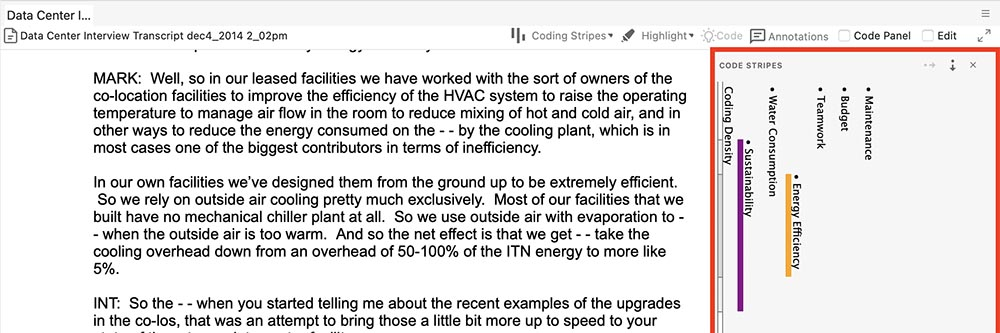
\includegraphics[keepaspectratio]{images/fig01b.jpg}}
\caption{Content analysis of interview using NVivo}
\end{figure}

The significance of content analysis lies in its ability to reveal the underlying messages and assumptions within media content. It allows researchers to move beyond surface-level descriptions to uncover the broader implications of media representations. For instance, by analyzing the content of political advertisements, researchers can assess how these ads influence voter behavior, contribute to political polarization, or reinforce gender stereotypes.

\subsection*{Studying Media Portrayals}\label{studying-media-portrayals}
\addcontentsline{toc}{subsection}{Studying Media Portrayals}

To illustrate the practical application of these concepts, consider a research project to study the portrayal of environmental issues in the media. In this study, the researcher might begin by selecting a set of news articles as artifacts. These articles are the primary data sources that will be systematically analyzed to address the research question.

The next step would involve identifying and coding the relevant attributes of these articles. For example, the researcher might code for the frequency of specific terms related to climate change, such as ``global warming,'' ``carbon emissions,'' or ``sustainability.'' The tone of the articles could also be coded as an attribute, with categories such as positive, neutral, or negative. Additionally, the researcher might analyze the framing of environmental issues, examining whether the articles emphasize the economic costs of addressing climate change or the moral imperative to act.

Once the artifacts and attributes have been coded, the researcher would analyze the content to uncover patterns and draw conclusions. For instance, the analysis might reveal that climate change is frequently framed as a distant, future problem rather than an immediate concern, potentially influencing public attitudes toward environmental policies. Alternatively, the analysis might show that certain news outlets consistently portray ecological activism negatively, contributing to public skepticism about environmental movements.

Engaging in this systematic analysis can generate insights that extend beyond the specific media content analyzed. They can contribute to broader discussions about media responsibility, public awareness, and the role of journalism in shaping societal values. Ultimately, research in mass communications serves as a critical tool for understanding the complex interactions between media and society, enabling us to make informed decisions about the media we consume and produce.

\section{Qualitative vs.~Quantitative}\label{qualitative-vs.-quantitative}

In mass communications research, understanding the distinction between qualitative and quantitative approaches is essential for grasping the breadth of methodologies available to scholars. These two primary approaches offer distinct pathways for exploring media messages, audience behaviors, and the societal impacts of communication. Each approach has strengths, limitations, and appropriate applications, depending on the research question and the data type being examined.

\subsection*{Qualitative Research}\label{qualitative-research}
\addcontentsline{toc}{subsection}{Qualitative Research}

\textbf{Qualitative research} is an interpretive approach that explores media phenomena' meaning, context, and complexity. This method is inherently flexible, allowing researchers to delve deeply into the nuances of how individuals and groups perceive, interpret, and experience media. Unlike quantitative research, which seeks to quantify and generalize findings across populations, qualitative research is concerned with understanding communication's rich, detailed, and often subjective aspects.

One of the primary objectives of qualitative research is to uncover the underlying meanings and implications of media content. This approach is particularly well-suited for investigating complex or culturally specific phenomena that cannot be easily reduced to numerical data. For example, a qualitative study might explore how different cultural groups interpret a controversial advertisement, revealing the varying emotional responses, interpretations, and cultural references that inform their understanding of the ad.

Standard methods used in qualitative research include in-depth interviews, focus groups, ethnography, and \textbf{content analysis}. In-depth interviews and focus groups involve direct interaction with participants, allowing researchers to gather detailed insights into their experiences and perspectives. On the other hand, ethnography involves the immersive study of media consumption within a specific cultural or social context, providing a holistic view of how media functions within that environment.

\textbf{Content analysis} in qualitative research involves systematically examining media content to identify patterns, themes, and implications. Unlike quantitative content analysis, which focuses on counting and categorizing content, qualitative content analysis aims to interpret the meaning behind the content. For example, a researcher might analyze the portrayal of gender roles in a series of television dramas, examining how these portrayals reinforce or challenge societal norms and expectations.

\textbf{Coding} is a crucial process in qualitative content analysis. It involves categorizing and organizing qualitative data into meaningful themes or groups, which helps researchers identify patterns and draw conclusions. Coding is an iterative process, often requiring multiple rounds of analysis as researchers refine their categories and interpretations. For instance, in analyzing news articles, a researcher might initially code the content based on broad themes like ``political bias'' or ``framing of economic issues'' and then refine these codes to capture more specific patterns within the data.

The strengths of qualitative research lie in its ability to provide deep, contextualized insights into media phenomena. However, it also has limitations. The findings from qualitative studies are often specific to the context in which the research was conducted, making it difficult to generalize to broader populations. Additionally, qualitative research can be time-consuming and requires a high level of interpretive skill, as the researcher must navigate the complexities of subjective data.

\subsection*{Quantitative Research}\label{quantitative-research}
\addcontentsline{toc}{subsection}{Quantitative Research}

\textbf{Quantitative research} is a systematic approach that emphasizes collecting and analyzing numerical data. This method is grounded in the principles of objectivity and replicability, making it well-suited for studies that aim to measure the extent, frequency, or correlations of specific phenomena. Quantitative research often tests hypotheses, identifies patterns, and establishes causal relationships between variables.

In mass communications, quantitative research typically involves surveys, experiments, and content analysis that quantifies aspects of media content. For example, a researcher might survey young adults to measure the relationship between social media usage and political engagement. The survey results would provide numerical data that can be analyzed statistically to identify trends and correlations.

One key advantage of quantitative research is its ability to produce statistically significant results that can be generalized to larger populations. This generalizability is achieved through random sampling and standardized data collection procedures, which help ensure that the findings are representative of the broader population. For instance, a nationwide survey on media consumption habits can provide insights into how different demographic groups engage with various media platforms, allowing researchers to draw conclusions about broader media trends.

\textbf{Experiments} are another standard method in quantitative research. In an experimental study, researchers manipulate one or more variables to observe their effects on a dependent variable. This method is particularly useful for establishing causal relationships. For example, an experiment might examine the impact of violent video game exposure on aggressive behavior by randomly assigning participants to play either a violent or non-violent video game and then measuring their subsequent behavior.

Quantitative \textbf{content analysis} involves systematically coding and counting media content to identify patterns or trends. Unlike qualitative content analysis, which focuses on interpretation, quantitative content analysis seeks to quantify the presence of specific elements within the content. For example, a researcher might analyze a sample of news broadcasts to determine the frequency of negative versus positive coverage of a political candidate. The results of this analysis could then be used to assess media bias or the potential impact of news coverage on public opinion.

Despite its strengths, quantitative research also has limitations. Its reliance on numerical data may overlook the complexities and subtleties of human experience that are often captured in qualitative research. Additionally, while quantitative research can identify correlations between variables, it does not always provide insights into the underlying reasons or mechanisms behind these relationships.

\subsection*{Mixed Methods Approach}\label{mixed-methods-approach}
\addcontentsline{toc}{subsection}{Mixed Methods Approach}

In recognition of the complementary strengths of qualitative and quantitative research, many scholars in mass communications adopt a \textbf{mixed methods} approach. This approach combines the depth and context of qualitative research with the generalizability and rigor of quantitative research, providing a more comprehensive understanding of the research question.

A mixed methods study might begin with qualitative research to explore a phenomenon in depth, followed by quantitative research to measure its prevalence or test specific hypotheses. For example, a researcher might conduct in-depth interviews with social media users to understand their experiences with online harassment. The themes identified in these interviews could then inform the design of a survey that measures the prevalence of these experiences across a larger population. By integrating qualitative and quantitative data, the researcher can gain a richer and more nuanced understanding of the issue.

Mixed methods research is precious in mass communications, where the complexity of media phenomena often requires both detailed exploration and broad measurement. This approach allows researchers to address the limitations of each method, providing a more holistic view of the research topic.

\chapter{Research Ethics and the IRB Process}\label{research-ethics-and-the-irb-process}

\section{The Evolution of Research Ethics in Social Science}\label{the-evolution-of-research-ethics-in-social-science}

The history of research ethics in social science is marked by a gradual but significant shift toward protecting human participants, driven by both high-profile ethical violations and the development of formal ethical guidelines. Early social science research often lacked clear ethical standards, resulting in studies that disregarded the rights and welfare of participants. This disregard for ethical considerations led to some of the most notorious examples of unethical research, spurring the creation of ethical frameworks that continue to guide researchers today.

\subsection*{Early Ethical Violations and the Call for Reform}\label{early-ethical-violations-and-the-call-for-reform}
\addcontentsline{toc}{subsection}{Early Ethical Violations and the Call for Reform}

The absence of formal ethical guidelines in the early days of social science research led to numerous studies that, by today's standards, would be considered profoundly unethical. Researchers often prioritized scientific knowledge above their participants' well-being and rights, resulting in severe ethical breaches. Three of the most notorious examples of unethical research during this period are the \textbf{Tuskegee Syphilis Study}, the \textbf{Milgram Experiments}, and the \textbf{Stanford Prison Experiment}.

\subsubsection*{The Tuskegee Syphilis Study (1932-1972)}\label{the-tuskegee-syphilis-study-1932-1972}
\addcontentsline{toc}{subsubsection}{The Tuskegee Syphilis Study (1932-1972)}

The Tuskegee Syphilis Study is one of the most egregious examples of unethical research in the history of social science and medical research. Conducted by the U.S. Public Health Service (PHS), the study initially aimed to observe the natural progression of untreated syphilis in African American men. The study began in 1932 in Macon County, Alabama, involving 600 African American men---399 of whom had syphilis and 201 who did not. The men were predominantly poor, uneducated sharecroppers who were not informed about the true nature of the study.

The men were told they were being treated for ``bad blood,'' a local term used to describe a variety of ailments, including syphilis. In reality, they were not given any proper treatment for syphilis. Even after penicillin became widely available in 1947 as a highly effective treatment for the disease, the researchers continued to withhold treatment from the participants, opting instead to observe the long-term effects of untreated syphilis. This decision was made despite the clear and unnecessary suffering it caused.

\begin{figure}
\centering
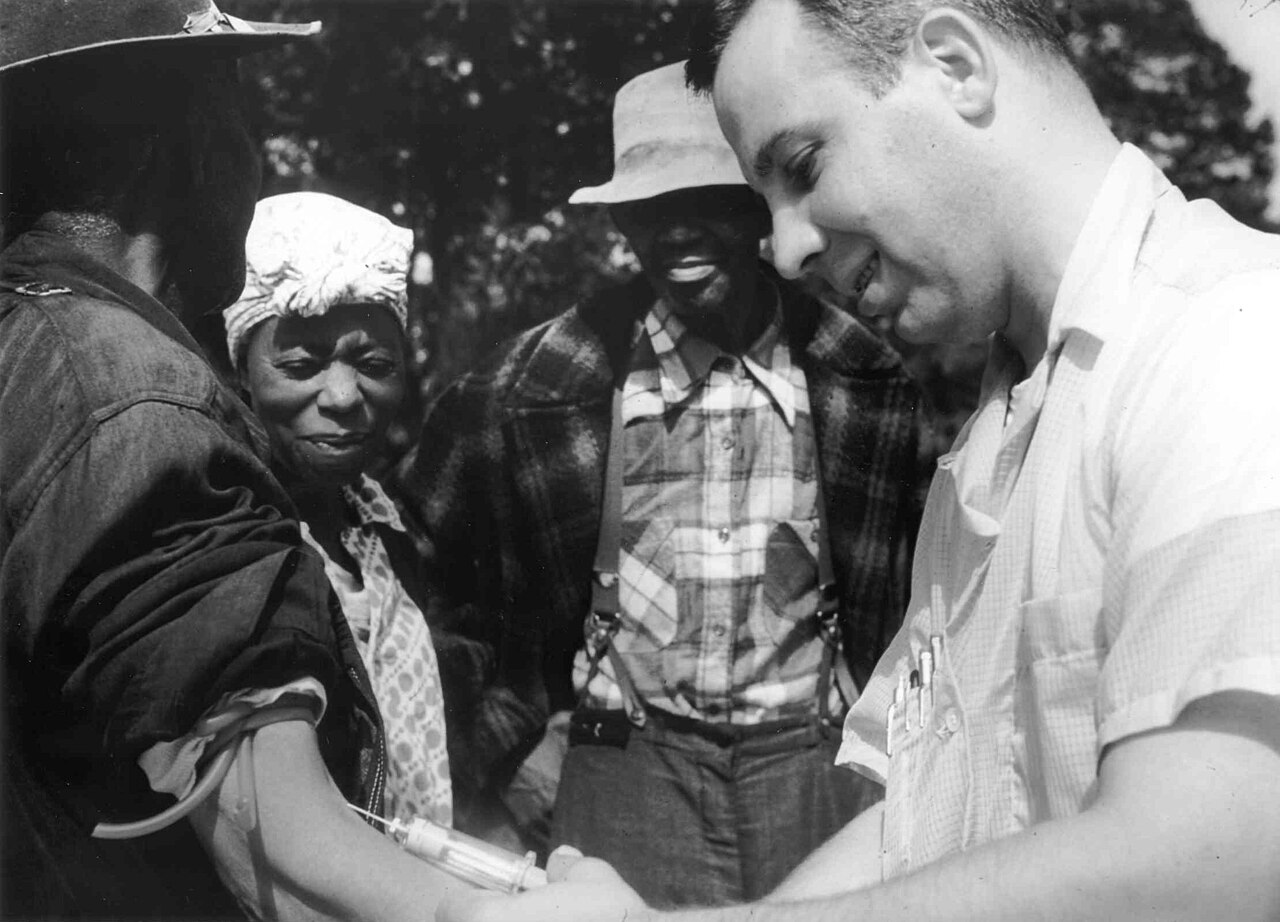
\includegraphics[width=1\linewidth,height=\textheight,keepaspectratio]{images/Tuskegee-syphilis-study.jpg}
\caption{A doctor draws blood from one of the Tuskegee test subjects.}
\end{figure}

The ethical violations in the Tuskegee Syphilis Study were profound. The participants were not informed that they had syphilis, nor were they informed that effective treatment was available. This lack of informed consent meant that the men were essentially used as human guinea pigs, suffering from a disease that could have been cured. The researchers' deception and exploitation of the participants, coupled with the decision to withhold treatment, resulted in needless suffering and death.

The study continued for 40 years before it was exposed by the media in 1972, leading to public outrage. The revelation of the Tuskegee Syphilis Study had far-reaching consequences, significantly undermining trust in the medical establishment, particularly among African Americans. It also led to significant reforms in research ethics, including establishing the National Research Act in 1974 and creating the National Commission for the Protection of Human Subjects of Biomedical and Behavioral Research, which produced the Belmont Report in 1979.

\subsubsection*{The Milgram Experiments (1961-1963)}\label{the-milgram-experiments-1961-1963}
\addcontentsline{toc}{subsubsection}{The Milgram Experiments (1961-1963)}

The Milgram Experiments, conducted by psychologist Stanley Milgram at Yale University in the early 1960s, were designed to investigate how individuals would obey authority figures, even when doing so conflicted with their conscience. The experiments were inspired by the atrocities committed during World War II, particularly the Holocaust, and sought to understand how ordinary people could commit or endorse such horrific acts under the influence of authority.

Participants in the Milgram Experiments were told they were participating in a study on learning and memory. They were assigned the role of a ``teacher,'' while another participant (actually an actor, or ``confederate'') was assigned the role of a ``learner.'' The teacher was instructed to administer electric shocks to the learner each time the learner made a mistake on a memory task. The shocks were fake, but the teacher was unaware of this. With each error, the shock's voltage was to be increased, and the learner (who was not actually being shocked) would act as if they were in severe pain, eventually begging for the experiment to stop.

\begin{figure}
\centering
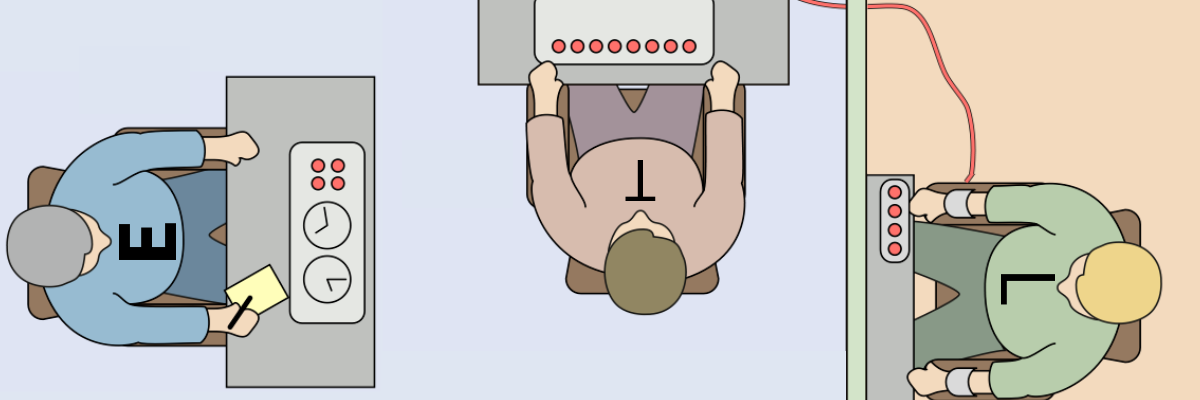
\includegraphics[width=1\linewidth,height=\textheight,keepaspectratio]{images/Milgram_experiment.png}
\caption{Participants by role. T = Teacher, L = Learner, E = Experimenter.}
\end{figure}

Despite the learner's pleas and the apparent severe pain they were causing, many participants continued to administer shocks when instructed by the experimenter, who was an authority figure in a lab coat. The experimenter would insist that the participant continue, often using prompts like ``The experiment requires that you continue'' or ``You have no other choice; you must go on.'' Astonishingly, a significant proportion of participants continued to administer shocks up to the highest voltage level, believing they were inflicting severe pain, even potentially lethal harm, on another person.

The Milgram Experiments highlighted the power of authority and the potential for ordinary individuals to commit extreme cruelty under its influence. However, they also raised serious ethical concerns, particularly regarding the use of deception and the psychological distress inflicted on the participants. Many of the participants experienced intense stress, guilt, and anxiety as a result of their actions during the experiment. They were deceived about the true nature of the study. They were not fully informed about the psychological risks involved, raising questions about informed consent and the ethical treatment of participants.

The ethical criticisms of the Milgram Experiments led to stricter regulations regarding the use of deception in research. They emphasized the importance of fully informing participants about the nature and risks of a study. The experiments are now widely cited as a pivotal example in discussions of research ethics, particularly concerning the balance between pursuing scientific knowledge and protecting research participants.

\subsubsection*{The Stanford Prison Experiment (1971)}\label{the-stanford-prison-experiment-1971}
\addcontentsline{toc}{subsubsection}{The Stanford Prison Experiment (1971)}

The Stanford Prison Experiment, led by psychologist Philip Zimbardo at Stanford University in 1971, is another infamous study that has been widely criticized for its ethical failings. The experiment aimed to investigate the psychological effects of perceived power, focusing on the struggle between prisoners and prison guards. To do this, Zimbardo and his team created a mock prison environment in the basement of the Stanford psychology building and recruited 24 male college students to participate.

The participants were randomly assigned to play the roles of either guards or prisoners. The guards were given uniforms, sunglasses, and batons, and were instructed to maintain order in the prison. The prisoners were stripped of their personal identity, dressed in smocks, and referred to by numbers rather than their names. The experiment was designed to last two weeks but was terminated after only six days due to the extreme and unethical behavior that quickly emerged.

\begin{figure}
\centering
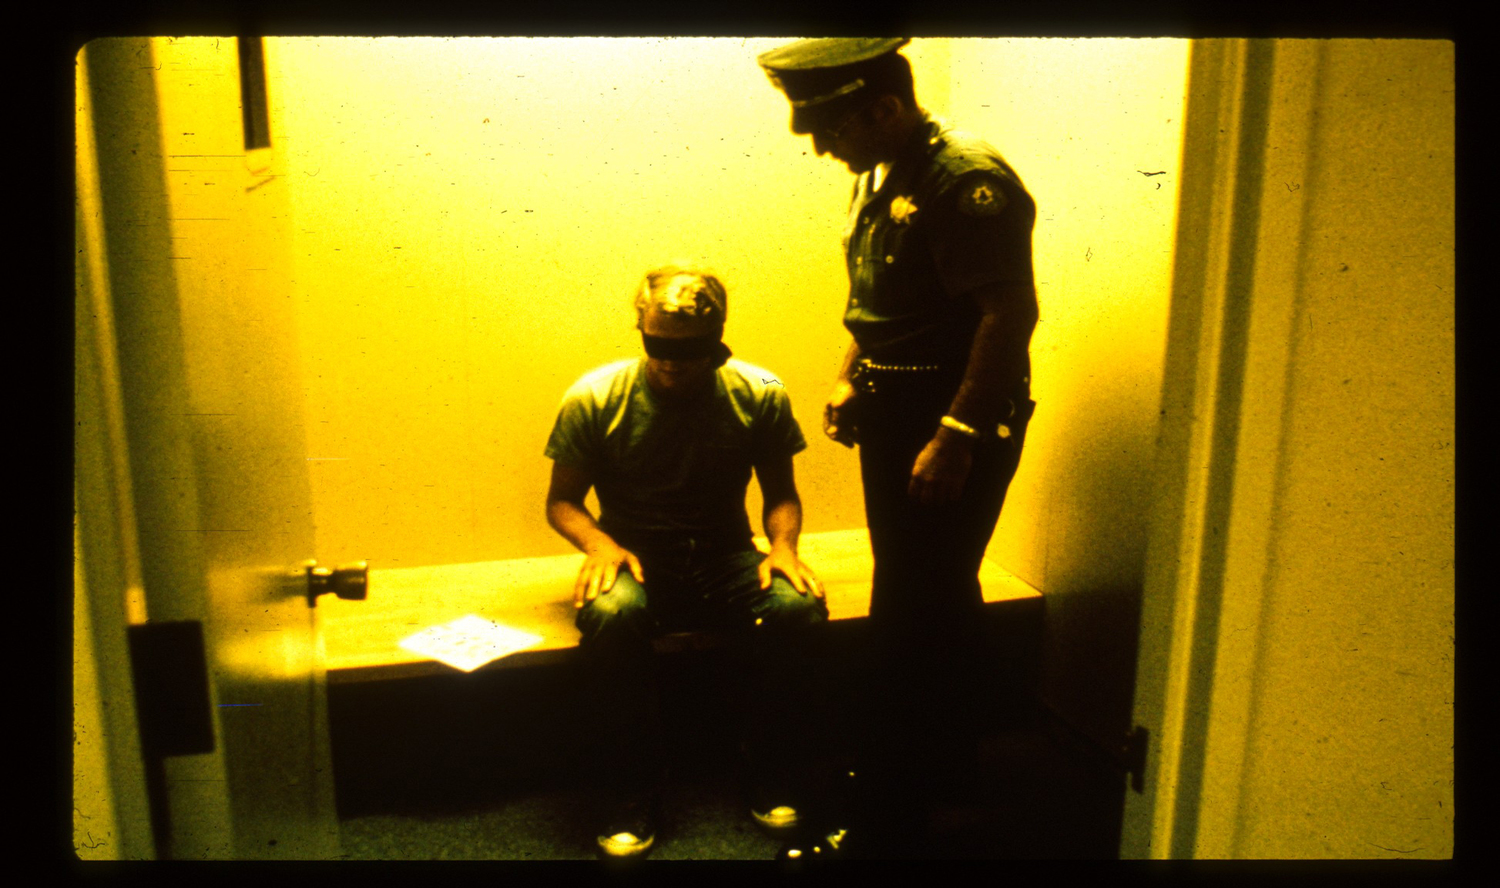
\includegraphics[width=1\linewidth,height=\textheight,keepaspectratio]{images/police-blindfolding.jpg}
\caption{Police blindfolding a research participant (\href{https://www.prisonexp.org/gallery}{prisonexp.org}).}
\end{figure}

Almost immediately, the guards began to exhibit abusive and authoritarian behavior toward the prisoners. They imposed harsh and degrading punishments, such as forcing prisoners to perform physical tasks like push-ups, depriving them of sleep, and humiliating them in various ways. The prisoners, in turn, became increasingly passive, depressed, and submissive. Some prisoners exhibited signs of severe emotional distress, and at least one had to be removed from the study early due to a mental breakdown.

Zimbardo, who served as both the lead researcher and the prison superintendent, did not intervene to stop the abusive behavior, arguing that the experiment needed to run its course to observe the psychological effects of the prison environment. However, the study spiraled out of control, causing significant psychological harm to the participants. The experiment was only halted when Zimbardo's then-girlfriend, psychologist Christina Maslach, visited the mock prison and expressed her strong objections to the conditions and the treatment of the participants.

The Stanford Prison Experiment has been heavily criticized for its lack of informed consent, the absence of measures to protect participants from harm, and the failure of the researchers to intervene when the situation became dangerous. The study demonstrated the ease with which people could engage in abusive behavior when placed in positions of authority, but it also highlighted the profound ethical responsibilities researchers have to protect their participants. The ethical failings of the Stanford Prison Experiment have since led to stricter regulations on the conduct of social science research, particularly concerning the treatment of participants and the need for rigorous oversight of studies involving potentially harmful situations.

\subsection*{The Emergence of Ethical Standards}\label{the-emergence-of-ethical-standards}
\addcontentsline{toc}{subsection}{The Emergence of Ethical Standards}

The history of social science research is punctuated by significant ethical violations that led to a growing demand for formalized ethical standards to protect human subjects. The widespread outrage and public awareness generated by unethical studies such as the Tuskegee Syphilis Study, the Milgram Experiments, and the Stanford Prison Experiment highlighted the urgent need for ethical guidelines in research. This demand for ethical reform catalyzed the development and adoption of foundational documents that have since shaped the ethical landscape of social science research.

\subsubsection*{The Nuremberg Code (1947)}\label{the-nuremberg-code-1947}
\addcontentsline{toc}{subsubsection}{The Nuremberg Code (1947)}

The first significant step toward formalizing ethical standards in research came with adopting the \textbf{Nuremberg Code} in 1947. This code was established in response to the atrocities committed by Nazi doctors during World War II, who conducted inhumane medical experiments on concentration camp prisoners without their consent. The subsequent Nuremberg Trials, where these doctors were prosecuted, underscored the need for clear ethical guidelines in medical research.

\begin{figure}
\centering
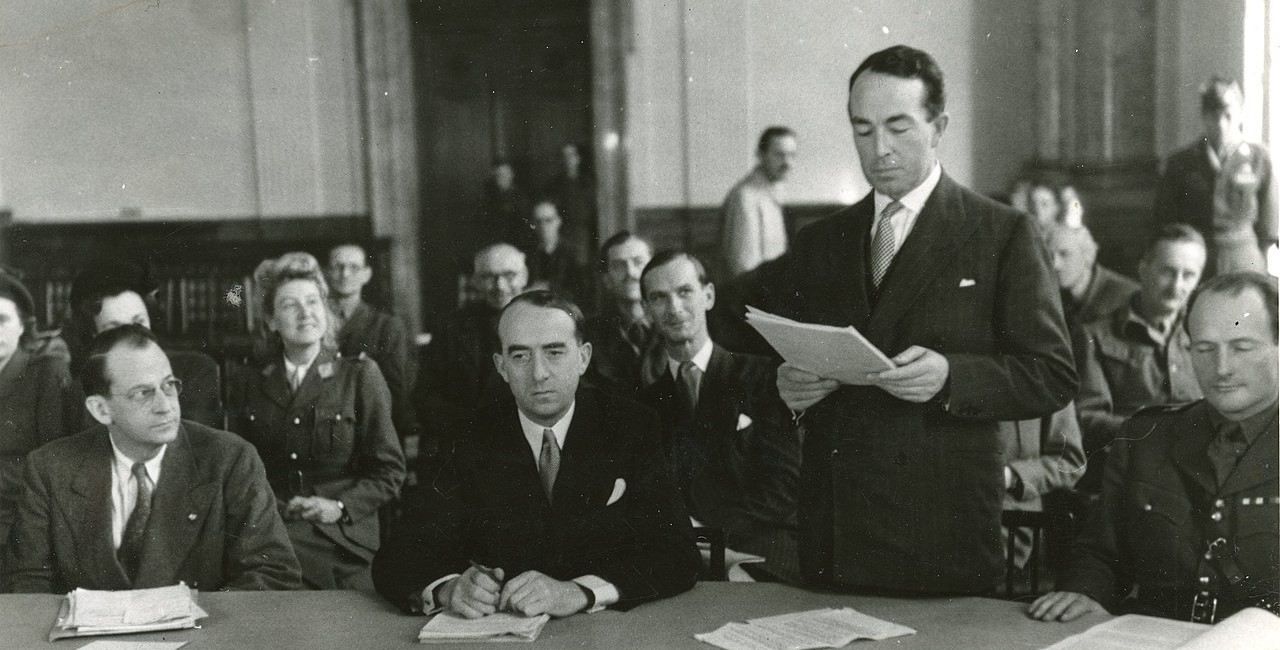
\includegraphics[width=1\linewidth,height=\textheight,keepaspectratio]{images/nuremberg-trial.jpg}
\caption{Handing over the indictment to the tribunal, 18 October 1945}
\end{figure}

The Nuremberg Code is composed of ten principles, which collectively emphasize the importance of voluntary consent, the necessity of avoiding unnecessary harm, and the obligation of researchers to terminate experiments that are likely to cause injury, disability, or death to participants. The key principles of the Nuremberg Code include:

\begin{enumerate}
\def\labelenumi{\arabic{enumi}.}
\item
  \textbf{Voluntary Consent:} The Code stipulates that ``the voluntary consent of the human subject is absolutely essential.'' This means that participants must be fully informed about the research's nature, purpose, and potential risks and must consent to participate without coercion.
\item
  \textbf{Beneficence and Non-Maleficence:} Researchers must design experiments that are likely to yield beneficial results for society and avoid unnecessary physical and mental suffering. This principle is rooted in the ethical obligation to maximize benefits and minimize harm.
\item
  \textbf{Right to Withdraw:} The Code grants participants the right to withdraw from a study if they feel uncomfortable or if the study risks their health or well-being.
\item
  \textbf{Scientifically Valid Research:} The Code mandates that research be based on prior animal experimentation and a sound understanding of the problem under study, ensuring that it is scientifically valid and justifiable.
\end{enumerate}

While the Nuremberg Code was initially focused on medical research, its principles laid the groundwork for ethical considerations in all research disciplines, including social science. The Code's emphasis on informed consent, beneficence, and protecting participants from harm became foundational concepts that would later influence the development of ethical standards in social science research.

\subsubsection*{The Declaration of Helsinki (1964)}\label{the-declaration-of-helsinki-1964}
\addcontentsline{toc}{subsubsection}{The Declaration of Helsinki (1964)}

Building on the ethical framework established by the Nuremberg Code, the \textbf{Declaration of Helsinki} was adopted by the World Medical Association in 1964. This declaration provided a comprehensive set of ethical guidelines for biomedical research involving human subjects and was particularly influential in shaping research practices across various disciplines, including social science.

The Declaration of Helsinki introduced several important ethical principles:

\begin{enumerate}
\def\labelenumi{\arabic{enumi}.}
\item
  \textbf{Informed Consent:} Expanding on the Nuremberg Code, the Declaration of Helsinki emphasizes the necessity of obtaining informed consent from research participants. It requires that participants be adequately informed about the study's aims, methods, potential benefits, risks, and the right to withdraw from the study at any time.
\item
  \textbf{Risk vs.~Benefit Analysis:} The Declaration requires researchers to carefully weigh the risks and benefits of their studies, ensuring that the potential benefits to society outweigh the risks to participants. This principle underscores the importance of beneficence in research ethics.
\item
  \textbf{Vulnerable Populations:} The Declaration highlights the need for special protections for vulnerable populations, such as children, pregnant women, and those with diminished autonomy. It acknowledges that these groups may be at greater risk of exploitation and harm in research settings.
\item
  \textbf{Ethical Review Committees:} The Declaration of Helsinki was one of the first documents to recommend the establishment of independent ethical review committees (now known as Institutional Review Boards, or IRBs) to oversee research studies. These committees ensure that studies are conducted ethically and that participants are protected from harm.
\end{enumerate}

Since its adoption, the Declaration of Helsinki has undergone several revisions, reflecting the evolving ethical challenges in research. Its influence extends beyond biomedical research, as many of its principles have been adapted and incorporated into ethical guidelines for social science research.

\subsubsection*{The National Research Act and the Belmont Report (1974-1979)}\label{the-national-research-act-and-the-belmont-report-1974-1979}
\addcontentsline{toc}{subsubsection}{The National Research Act and the Belmont Report (1974-1979)}

The formal codification of social science research ethics in the United States began in earnest with the passage of the \textbf{National Research Act} in 1974. This legislation was enacted in response to growing concerns about the treatment of research participants, particularly in the wake of the Tuskegee Syphilis Study, which had been exposed just two years earlier.

The National Research Act established the \textbf{National Commission for the Protection of Human Subjects of Biomedical and Behavioral Research}, a body tasked with developing ethical guidelines for human subject research. The commission's most influential contribution was the 1979 publication of the Belmont Report.

The Belmont Report outlines three fundamental ethical principles that continue to guide social science research:

\begin{enumerate}
\def\labelenumi{\arabic{enumi}.}
\item
  \textbf{Respect for Persons:} This principle encompasses informed consent and the recognition of the autonomy of research participants. It asserts that individuals should be treated as autonomous agents capable of making their own decisions about whether to participate in research. For those with diminished autonomy, such as children or individuals with cognitive impairments, additional protections must be in place.
\item
  \textbf{Beneficence:} The principle of beneficence requires researchers to minimize potential harm to participants while maximizing the potential benefits of the research. This principle involves carefully assessing risks and benefits and implementing measures to protect participants from harm.
\item
  \textbf{Justice:} The principle of justice addresses the fair distribution of the benefits and burdens of research. It ensures that no group of people is unfairly burdened by the risks of research or unfairly excluded from its benefits. This principle is particularly relevant in addressing historical injustices in research, such as exploiting marginalized communities.
\end{enumerate}

The Belmont Report has profoundly impacted the ethical conduct of research in the United States and beyond. Its principles are embedded in federal regulations, such as the Common Rule, which governs research involving human subjects in the United States. The Belmont Report also serves as a foundational document for ethical guidelines in various disciplines, including social science.

\subsubsection*{The Impact and Legacy of Emerging Ethical Standards}\label{the-impact-and-legacy-of-emerging-ethical-standards}
\addcontentsline{toc}{subsubsection}{The Impact and Legacy of Emerging Ethical Standards}

Adopting the Nuremberg Code, the Declaration of Helsinki, and the Belmont Report marked significant milestones in formalizing ethical standards in research. These documents have had a lasting impact on the conduct of social science research, ensuring that the rights and welfare of research participants are prioritized.

The ethical principles articulated in these documents---voluntary consent, informed consent, beneficence, and justice---have become the cornerstones of research ethics. They have shaped the policies and practices of research institutions, guided the development of ethical review processes, and influenced how researchers design and conduct studies.

Moreover, establishing independent ethical review boards, as the Declaration of Helsinki and the Belmont Report recommended, has become a standard research practice. These boards play a critical role in safeguarding the rights and well-being of research participants by reviewing study protocols, assessing potential risks and benefits, and ensuring that ethical principles are upheld.

As social science research continues to evolve, the ethical challenges facing researchers also change. New technologies, such as digital data collection, social media research, and artificial intelligence, present novel ethical dilemmas requiring ongoing reflection and adaptation of ethical standards. Nevertheless, the foundational principles established by the Nuremberg Code, the Declaration of Helsinki, and the Belmont Report remain central to the ethical conduct of research, providing a framework for addressing emerging ethical issues in social science.

\section{Navigating the IRB Process}\label{navigating-the-irb-process}

Navigating the Institutional Review Board (IRB) process is critical to conducting ethical research involving human participants. The IRB is responsible for reviewing research proposals to ensure that they comply with ethical standards and protect the rights and welfare of participants. As a researcher, particularly within the context of Southern Illinois University Edwardsville (SIUE), understanding the intricacies of this process is essential for gaining approval and conducting your research responsibly. This section will thoroughly explore the key components of the IRB process at SIUE, including creating consent forms, debriefing participants, assessing potential harm, offering incentives, and understanding the submission protocols.

\href{https://www.siue.edu/compliance/training/}{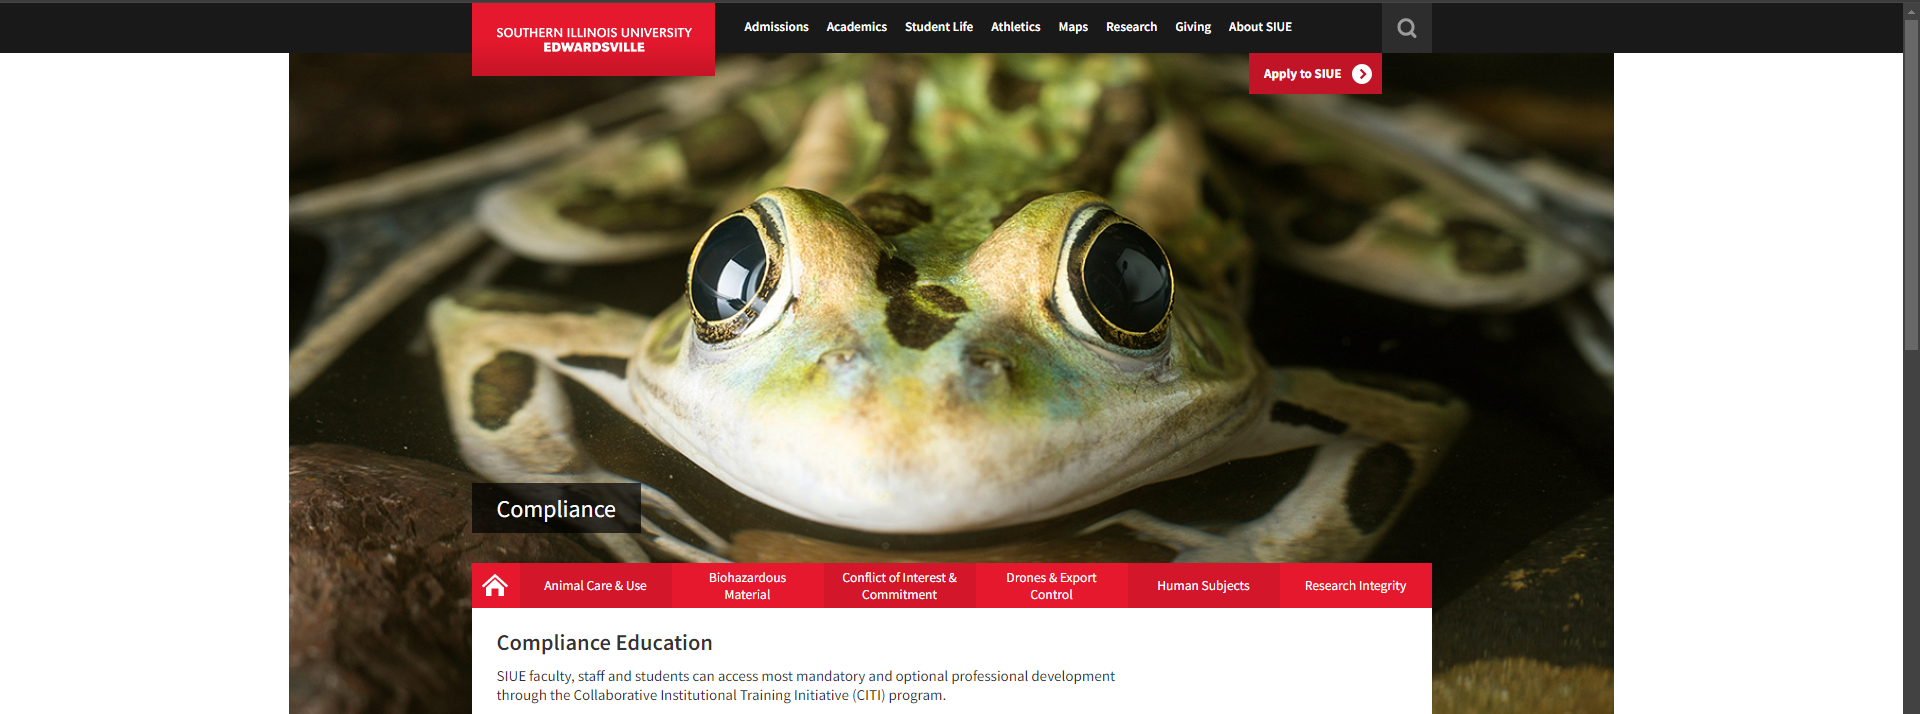
\includegraphics[width=1\linewidth,height=\textheight,keepaspectratio]{images/compliance-education.png}}

\subsection*{Completing CITI Certification}\label{completing-citi-certification}
\addcontentsline{toc}{subsection}{Completing CITI Certification}

\begin{enumerate}
\def\labelenumi{\arabic{enumi}.}
\item
  \textbf{Use the SIUE \href{https://www.citiprogram.org/Shibboleth.sso/Login?target=https\%3A\%2F\%2Fwww.citiprogram.org\%2FSecure\%2FWelcome.cfm?inst=551&entityID=https\%3A\%2F\%2Fsts.windows.net\%2F99f37d21-0b5c-43ea-9103-e16f02f5aecf\%2F}{single sign-on page} to enter your SIUE e-id and password.}

  If this doesn't work, try the following:

  \begin{itemize}
  \item
    Go to the CITI Program page.
  \item
    Click on ``Log in''
  \item
    Then, at the top of the page, click on ``Log In Through My Organization.'' (If you have already logged in before, depending on your browser, you may be taken directly to signing in with your e-id and password, if so, proceed to \#2 below.)
  \item
    Choose Southern Illinois University Edwardsville from the drop-down box.
  \end{itemize}

  \begin{figure}
  \centering
  
\includegraphics[width=1\linewidth,height=\textheight,keepaspectratio]{images/citi-org-login.png}
  \caption{Organization Single Sign On (SSO) screen for CITI}
  \end{figure}

  \begin{itemize}
  \item
    If this is your first time logging into CITI using your SSO, it will ask you to choose one of the following:

    \begin{enumerate}
    \def\labelenumii{\arabic{enumii}.}
    \item
      I already have a CITI program account or
    \item
      I don't have a CITI program account and need one created. Note: If you select this option, the next step will ask you to press a button that says ``Create new CITI Program Account.''
    \end{enumerate}
  \end{itemize}
\item
  At the top left side of the page, you should see ``Welcome, {[}and your name{]}.'' In the middle of the page, under ``Institutional Courses,'' Click on the ``View Course'' button.
\item
  You should now see a list of ``Active Courses'' and Southern Illinois University Edwardsville at the top.
\end{enumerate}

\begin{quote}
\textbf{IMPORTANT: If courses are not listed, scroll to the bottom of the page and click ``Add a Course.''}
\end{quote}

\begin{figure}
\centering

\includegraphics[width=1\linewidth,height=\textheight,keepaspectratio]{images/citi-add-a-course.png}
\caption{Click the circled link to add a new course.}
\end{figure}

\begin{quote}
\textbf{Then scroll down until you see a question relating to compliance topics (you only need Human Subjects for this course).}
\end{quote}

\begin{figure}
\centering
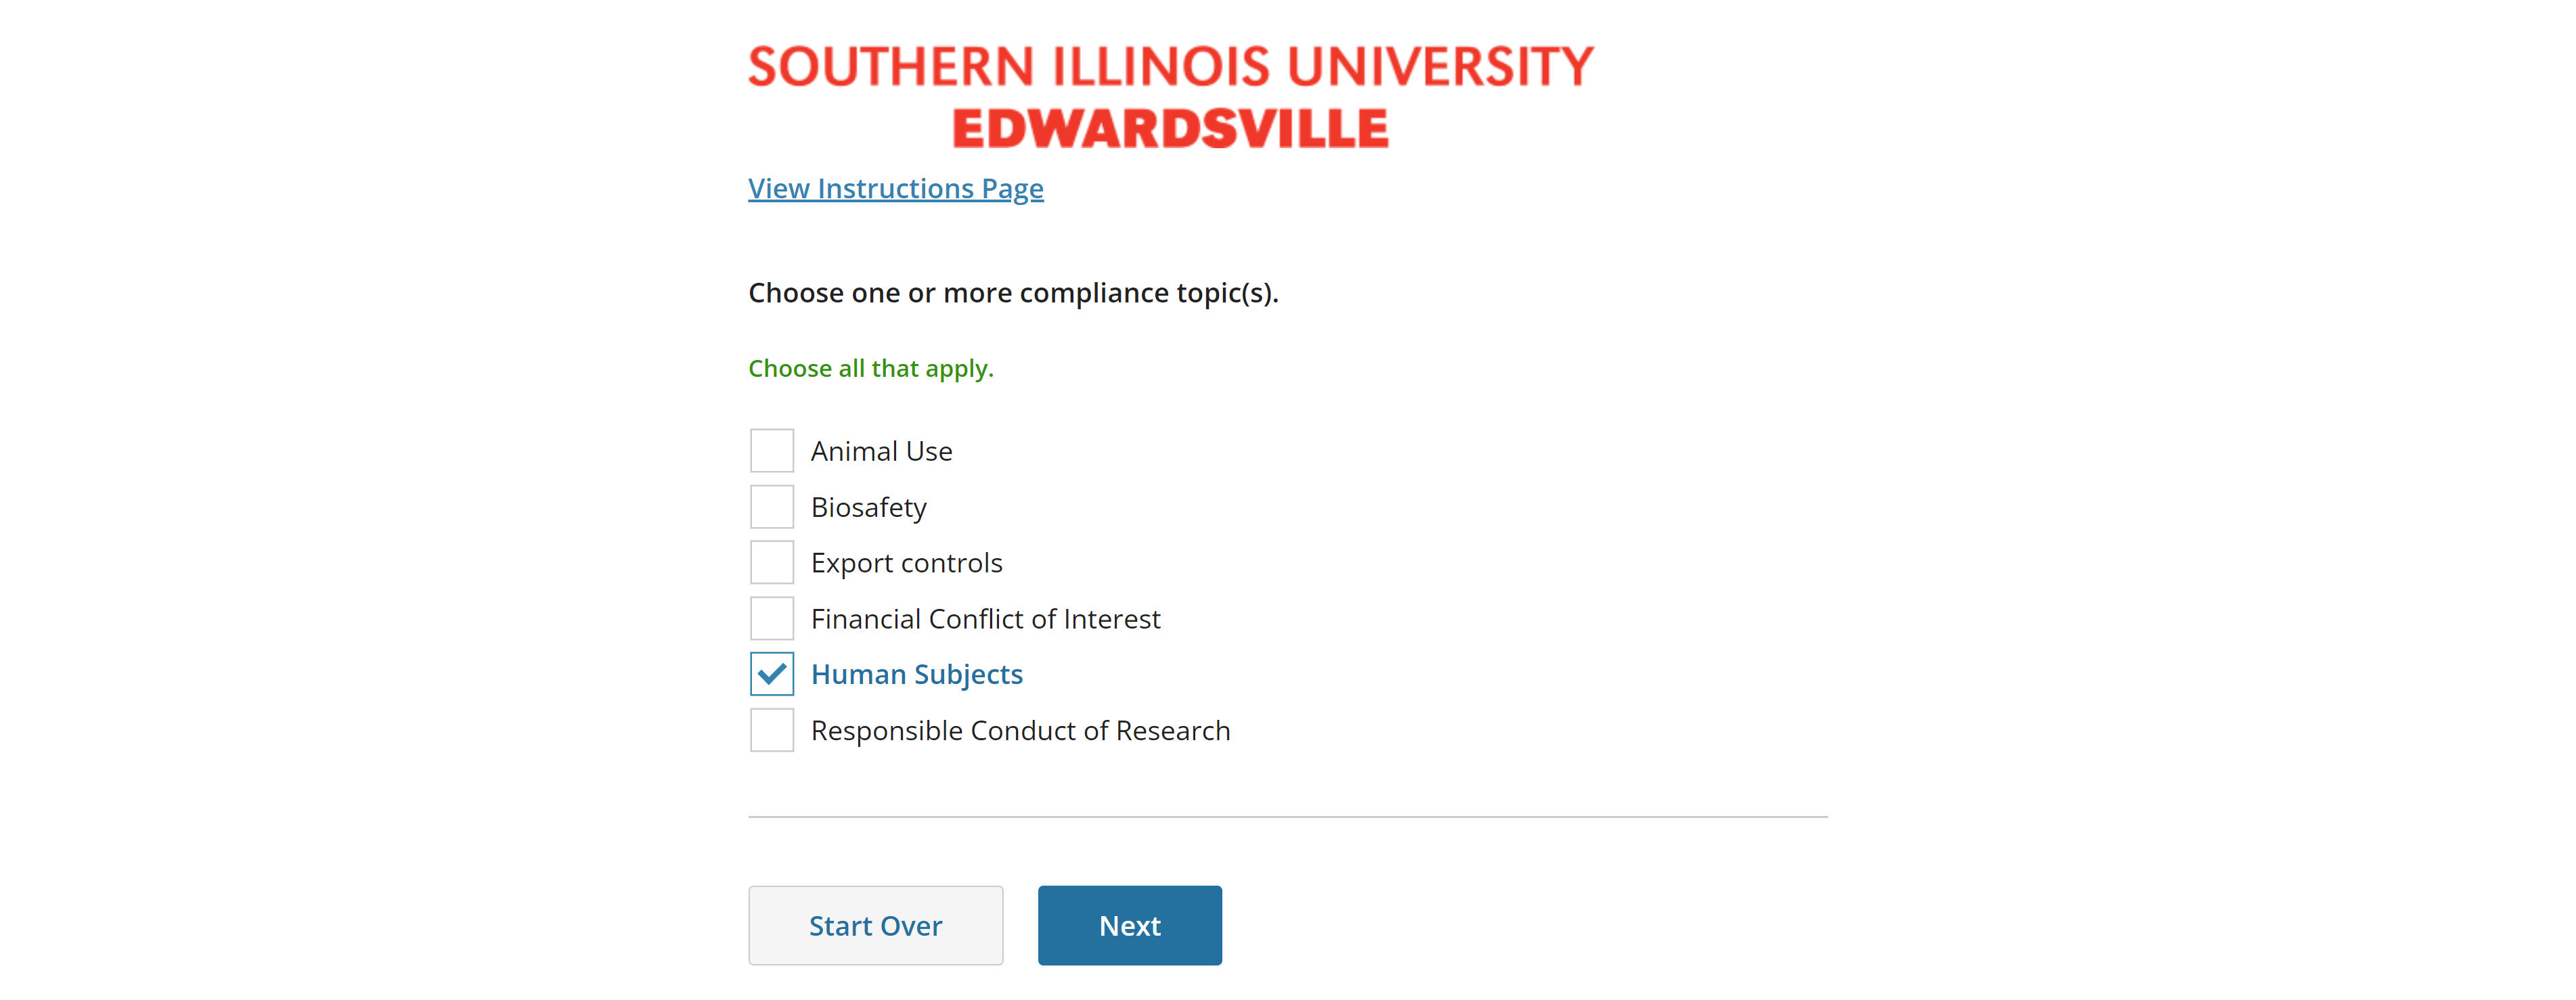
\includegraphics[width=1\linewidth,height=\textheight,keepaspectratio]{images/citi-topics.png}
\caption{CITI compliance topics.}
\end{figure}

\begin{quote}
\textbf{Then select your course (you want the Social behavioral student course).}
\end{quote}

\begin{figure}
\centering
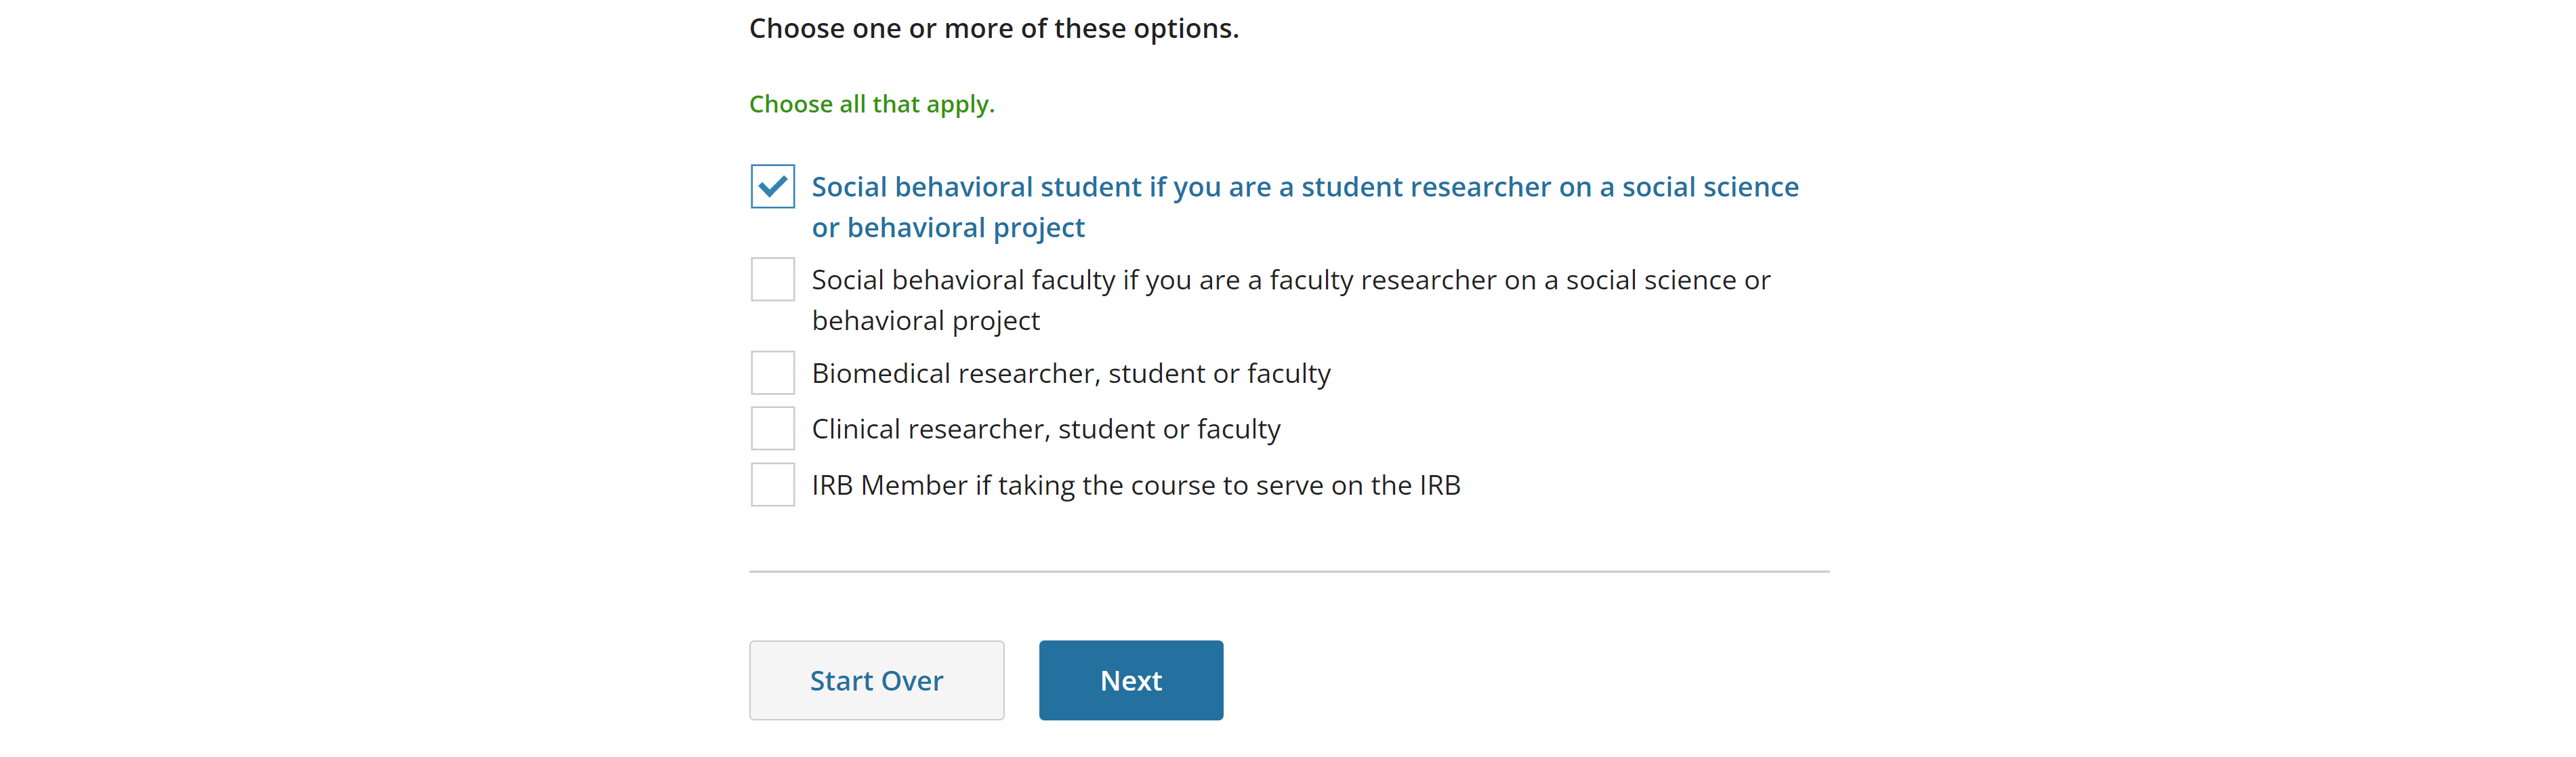
\includegraphics[width=1\linewidth,height=\textheight,keepaspectratio]{images/citi-courses.png}
\caption{CITI course selection.}
\end{figure}

\begin{enumerate}
\def\labelenumi{\arabic{enumi}.}
\setcounter{enumi}{3}
\item
  After answering the questions, scroll to the bottom of the page and click \textbf{``Next.''} This will take you to the stage selection page. Choose Stage 1 if this is your first time getting IRB Certified as a student. Choose Stage 2 if this is a refresher, and click ``\textbf{Submit.''}
\item
  You are now ready to complete the course(s). Once completed, the CITI system will provide you with a Certificate of Completion for each course. You may print and save a copy for your records.
\end{enumerate}

\subsection*{Retrieving Your CITI Certificate}\label{retrieving-your-citi-certificate}
\addcontentsline{toc}{subsection}{Retrieving Your CITI Certificate}

Once you have completed your CITI certification, you can review the course or view your record. If you click on the button to view your record, you will be presented with two options: completion report and completion certificate. You will be able to add your certificate to LinkedIn. You can access that through this page's ``View/Print'' button.

\begin{figure}
\centering
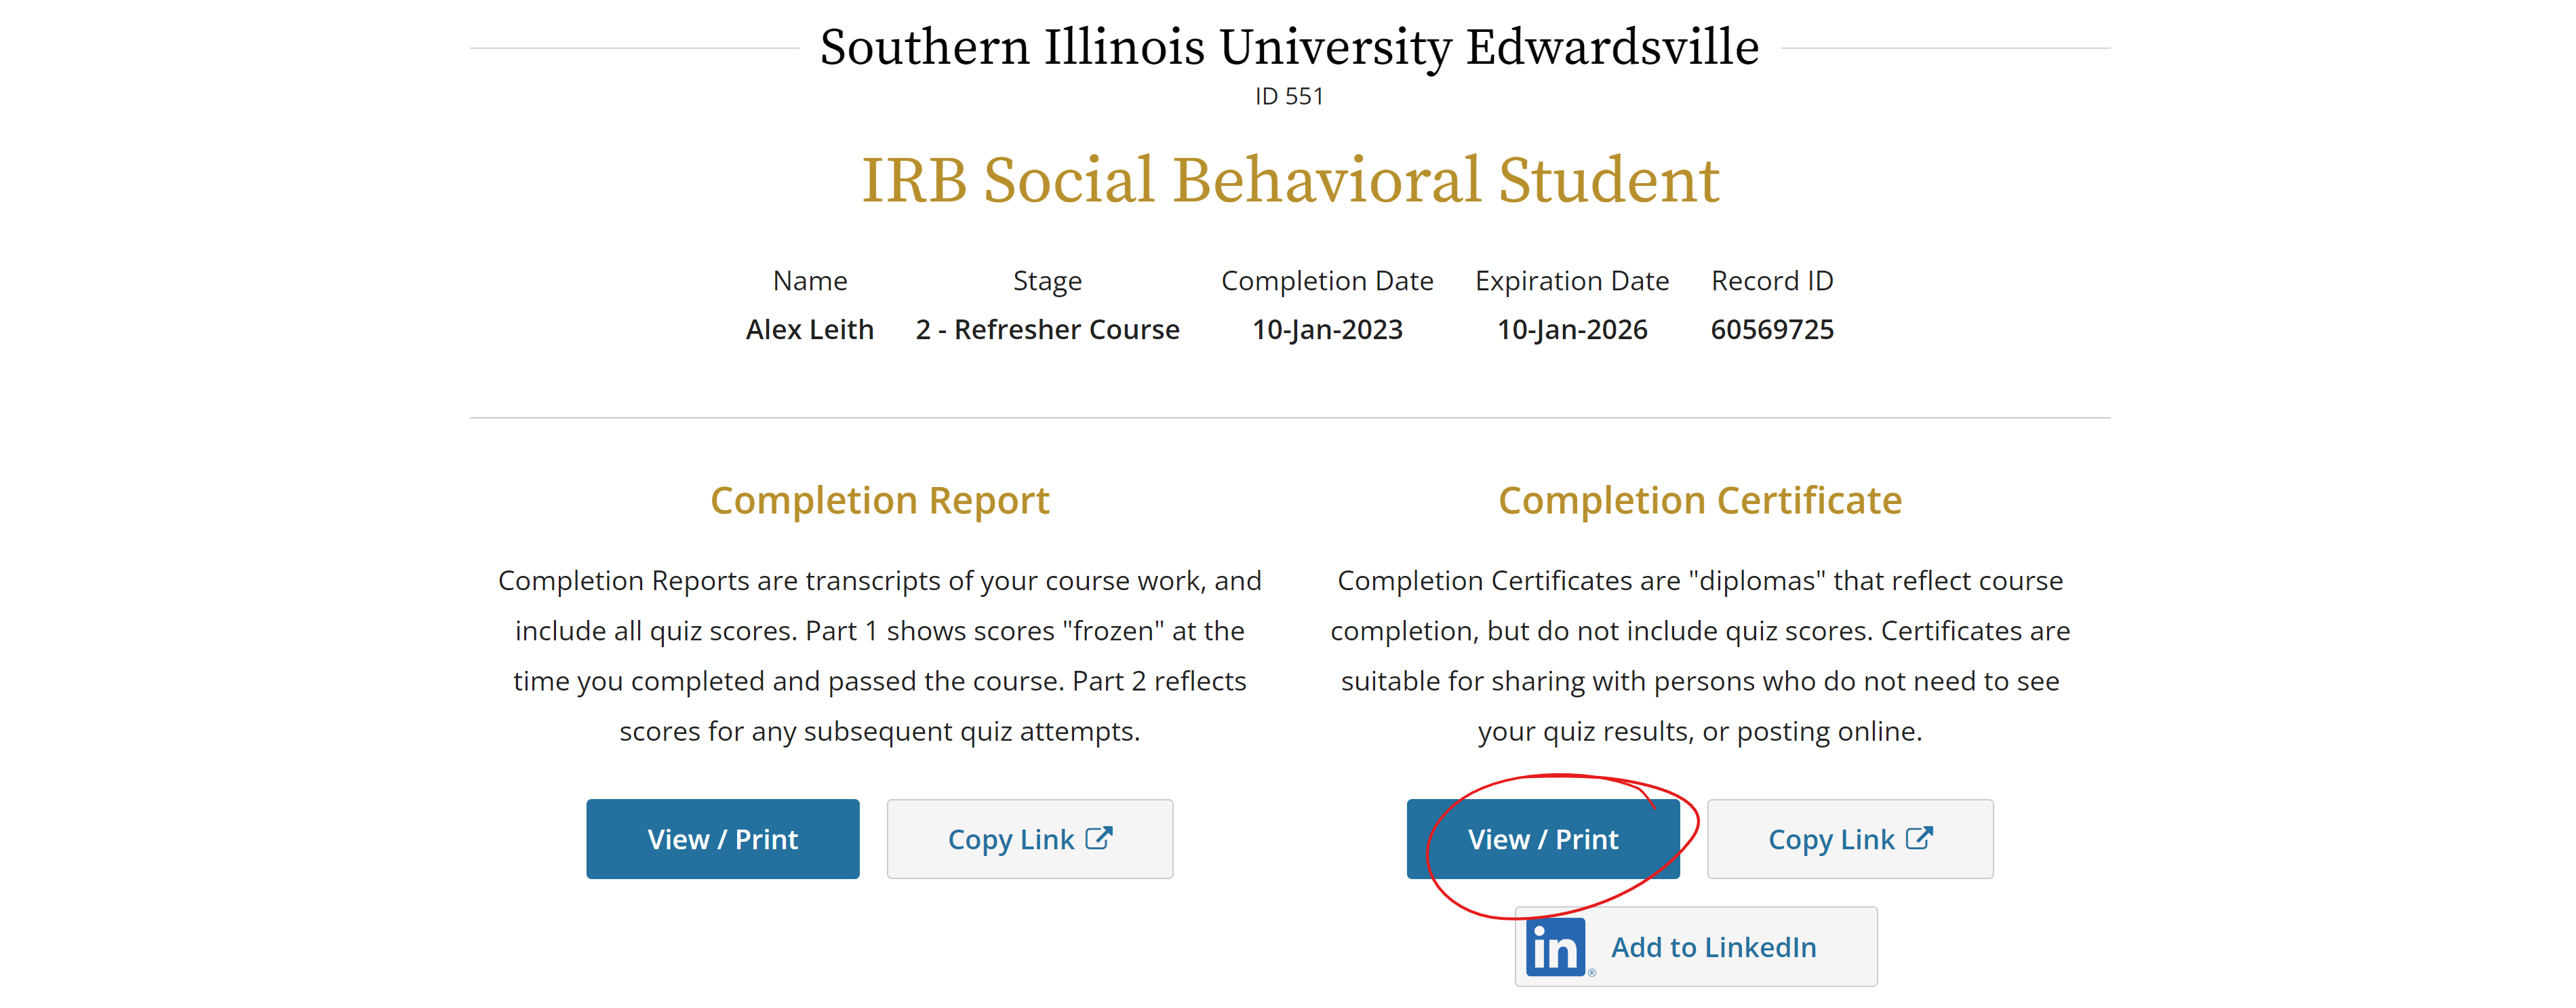
\includegraphics[width=1\linewidth,height=\textheight,keepaspectratio]{images/citi-cert-link.png}
\caption{Link circled to access IRB certification.}
\end{figure}

Whether you access your IRB certificate through the CITI website or from your LinkedIn profile, it will be identical. Most research courses or teams will request a copy of your CITI Certificate to keep on record since it is commonly requested when completing an IRB proposal.

\href{https://www.linkedin.com/in/apleith/details/certifications/}{\pandocbounded{
\includegraphics[keepaspectratio]{images/irb-cert.png}}}

\subsection*{Completing IRB Proposal}\label{completing-irb-proposal}
\addcontentsline{toc}{subsection}{Completing IRB Proposal}

You will submit a proposal to SIUE's Institutional Review Board (IRB) through Kuali's protocols section. Once you have signed into Kuali, you can create a new proposal by selecting the ``\textbf{+ New Protocol}'' button in the top right of the page. You will only need a single new protocol, whether a solo researcher or a group researcher.

In the \textbf{General Information} section, the creator of the proposal should be the principal investigator, and their lead unit should be their department; if you are an employee or the department for which the research is being conducted, if you are a student doing research for a course or for a faculty member. The ``Study Title'' is a general name that summarizes the research you will be conducting. The Study Title and the eventual paper title can be different. Finally, for this course, the project is student-led.

For the \textbf{SIUE Personnel} section, you must include the names of all participants at SIUE. You must make sure to include an answer to all sections. You select the ``\textbf{+ Add Line}'' button to add additional researchers. The pencil icon lets you edit the person's information. From there, you must add information to each field. Required information may include a copy of IRB Certificates. You must also grant Access to all participants, including the professor if they supervise the research. There are sections that include researcher experience and researcher involvement that must be answered, even if there is no experience or limited involvement. You select No for external researchers unless you are also working with scholars outside of your university.

\href{https://siue.kuali.co/protocols/portal/protocols}{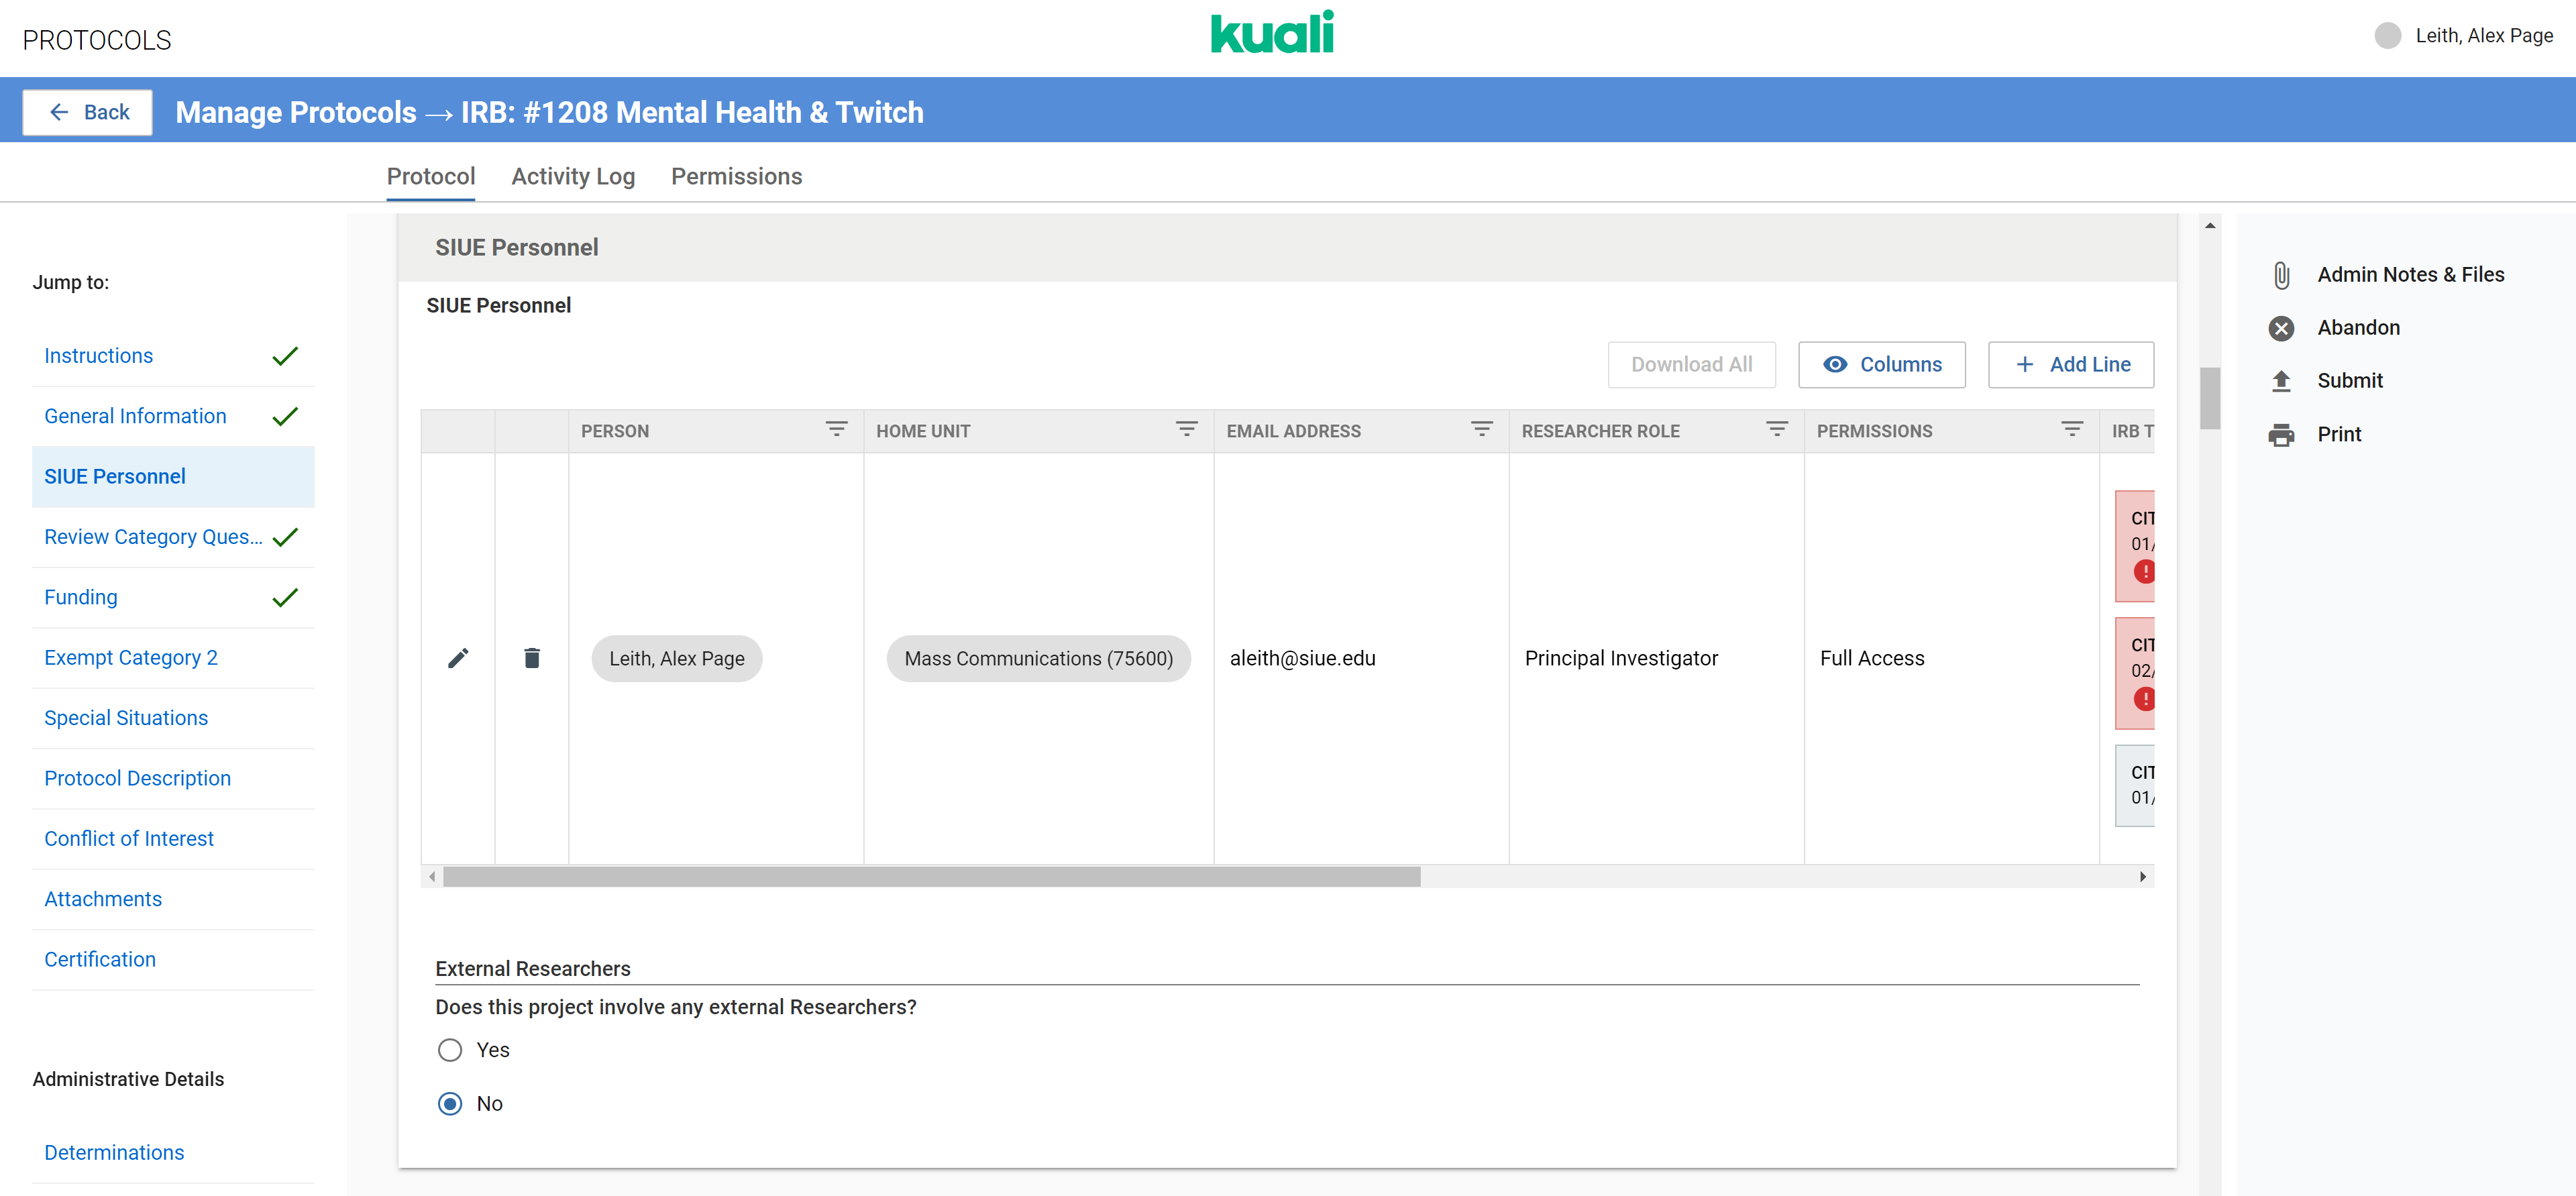
\includegraphics[width=1\linewidth,height=\textheight,keepaspectratio]{images/siue-personnel.png}}

The next significant stage for discussion is the ``\textbf{Review Category Questions (GQ)}'' section. The GQ section allows you to identify how strict the IRB must be with your study. The less potential harm, the simpler it is to approve your research. For this course, we are strictly doing exempt projects. Exempt projects generally exclude protected classes or projects that may cause atypical harm. If you are doing survey research, you select exempt status and Category 2 since this is a survey procedure. You should have learned the different categories curing your CITI IRB certification process.

\begin{figure}
\centering
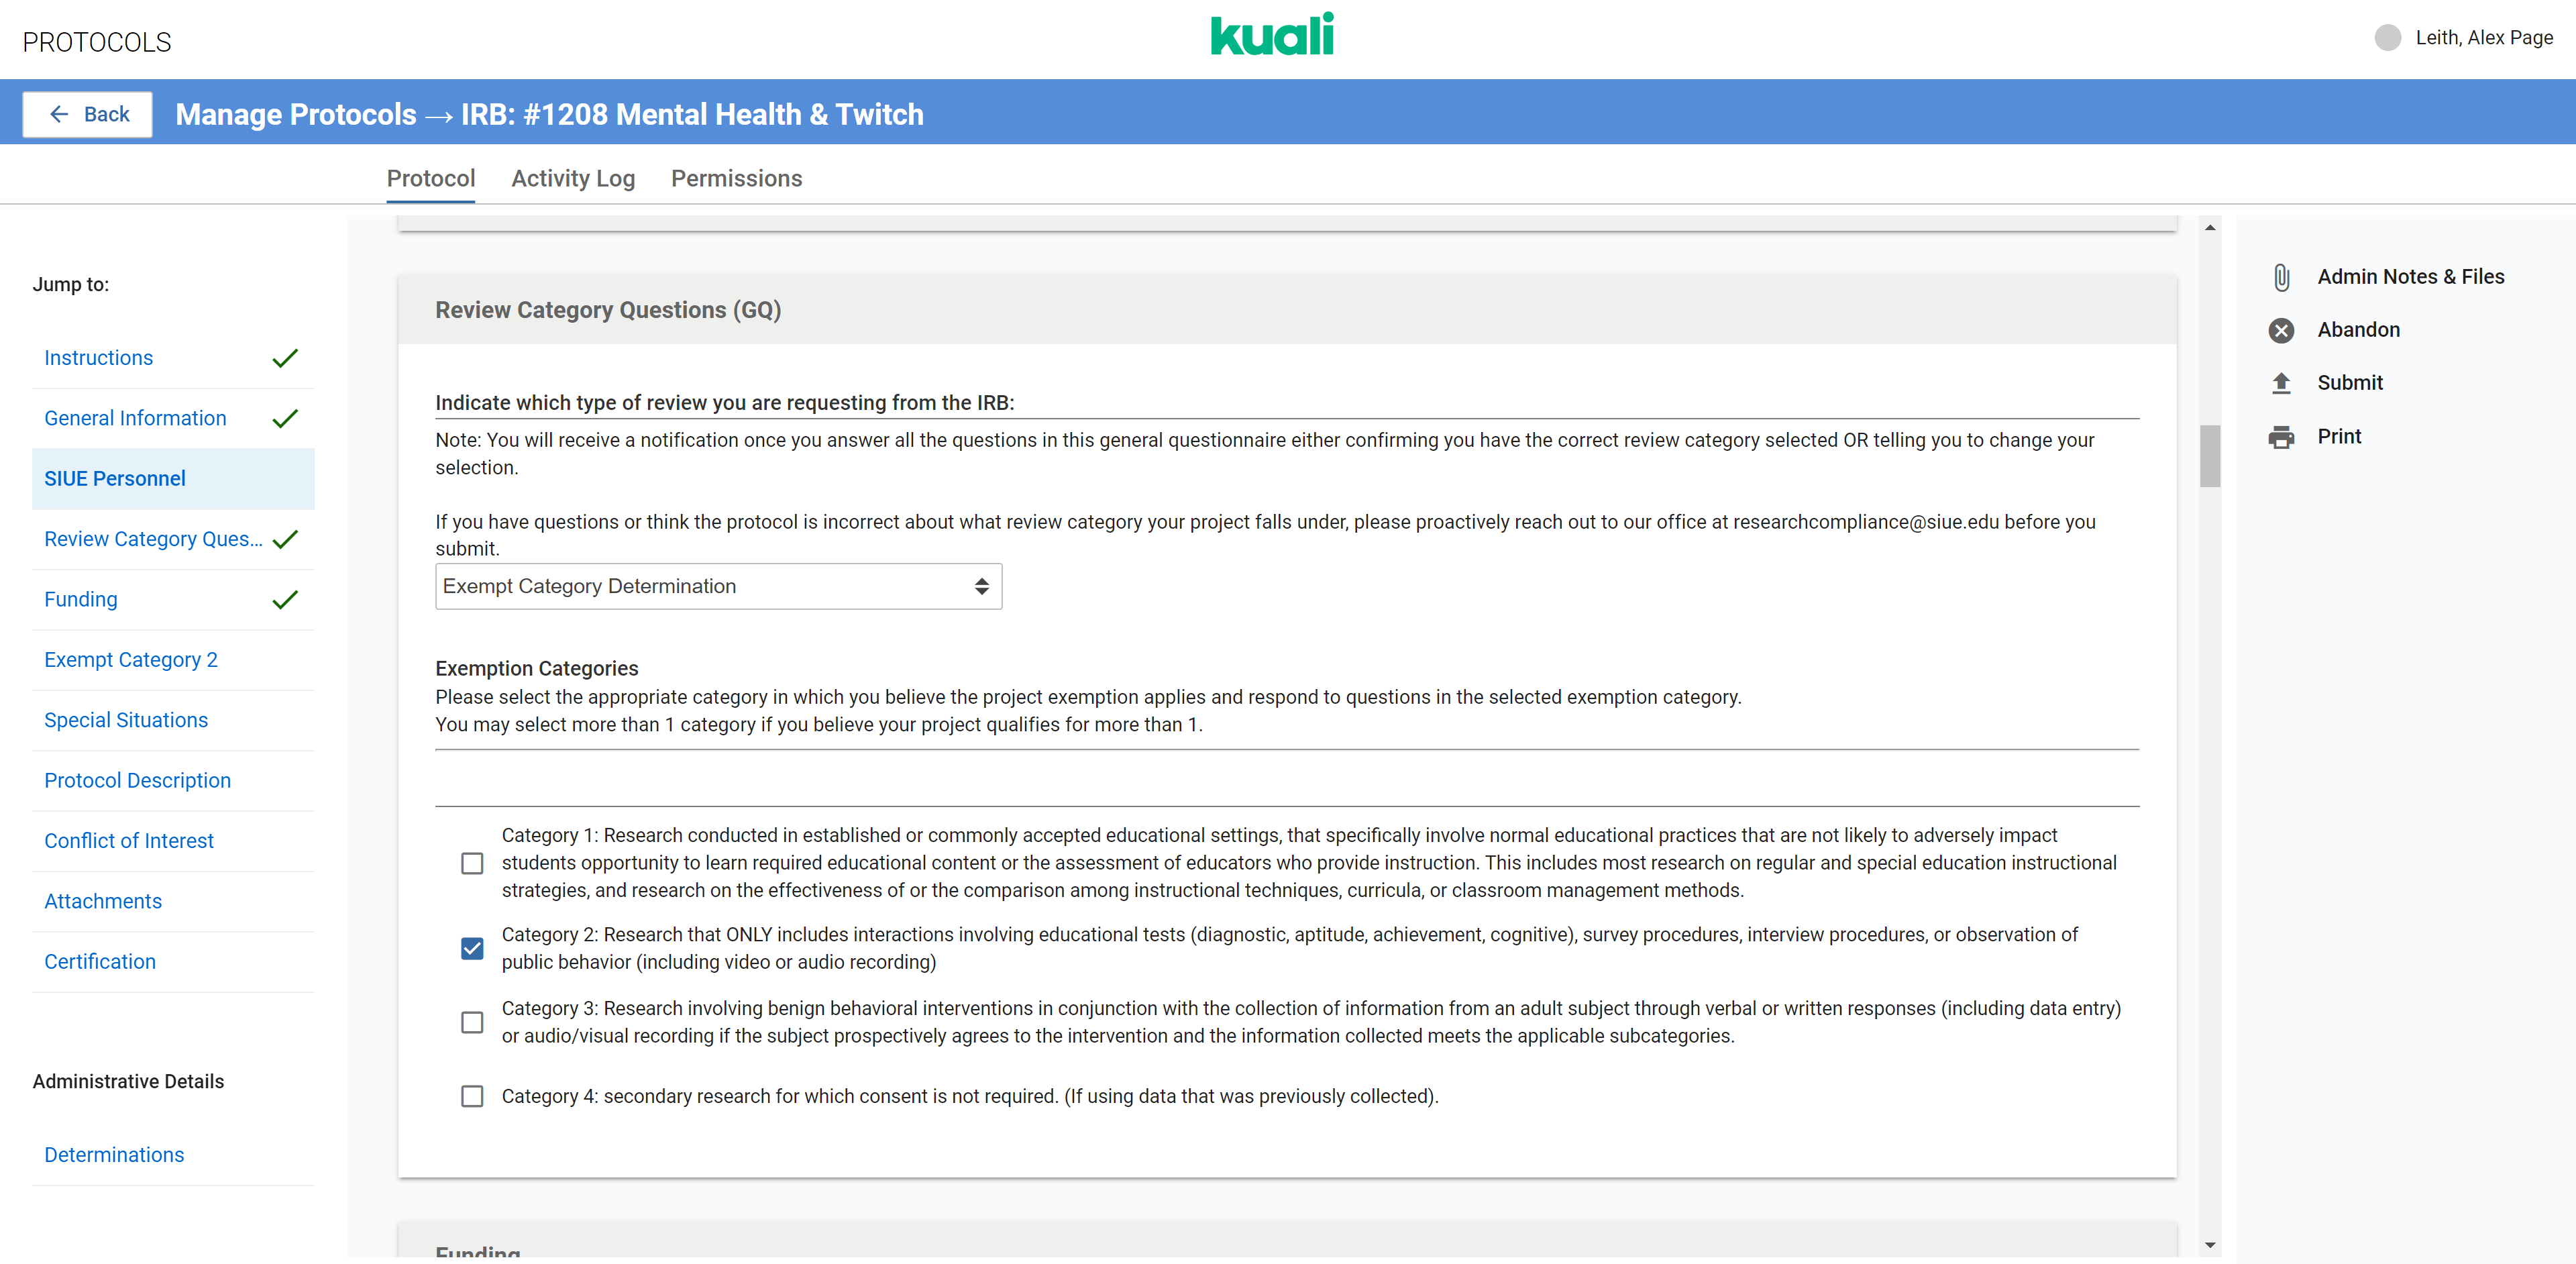
\includegraphics[width=1\linewidth,height=\textheight,keepaspectratio]{images/kuali-exempt.png}
\caption{Kuali section for select exempt status.}
\end{figure}

The following sections are text fields that require you to explain the process of your project. You must ensure that your answers are complete and thorough. It is better to over-explain than under-explain. Further, it is better to answer ``N/A'' than to leave a field blank. Please review SIUE's \href{https://www.siue.edu/compliance/human-subjects/pdf/IRBProtocolGuidance.pdf}{IRB Protocol Guide} with questions regarding these sections.

You will eventually reach the ``\textbf{Attachments}'' section of the proposal. For the attachments section, you must include your consent forms, recruitment documents, and research materials (e.g., survey questions).

\subsection*{Developing Consent Forms}\label{developing-consent-forms}
\addcontentsline{toc}{subsection}{Developing Consent Forms}

\textbf{Consent forms} are a cornerstone of ethical research, providing participants with all the necessary information to make an informed decision about their involvement in the study. At SIUE, creating a consent form must align with the ethical guidelines and requirements stipulated by the IRB. The consent form must clearly outline the study's purpose, procedures, potential risks, benefits, and measures to ensure participant confidentiality.

Creating a consent form is more than just completing a document; it involves crafting a communication tool that genuinely informs participants. According to the SIUE guidelines, the language used in consent forms should be clear, concise, and devoid of technical jargon that might confuse participants (IRB Protocol Guidance, 2023). For example, it is crucial to break down the information into understandable segments when explaining complex procedures, ensuring that participants fully comprehend their participation.

Moreover, the consent form must explicitly state that participation is voluntary and that participants can withdraw from the study at any point without any negative consequences. This ensures that participants are not coerced or unduly influenced to continue their involvement against their will. The \textbf{2023 IRB Protocol Guidance} document from SIUE emphasizes that consent forms should include detailed information on how participants can withdraw and what steps will be taken to handle their data if they choose to do so (IRB Protocol Guidance, 2023).

\subsection*{Developing Recruitment Materials}\label{developing-recruitment-materials}
\addcontentsline{toc}{subsection}{Developing Recruitment Materials}

Recruitment materials play a crucial role in attracting participants to a research study. These materials must be designed to clearly communicate the purpose of the study, the expectations for participation, and the benefits of involvement while adhering to ethical standards. At SIUE, recruitment materials must be developed per the guidelines the Institutional Review Board (IRB) set forth, ensuring transparency and respect for potential participants' autonomy.

\begin{figure}
\centering
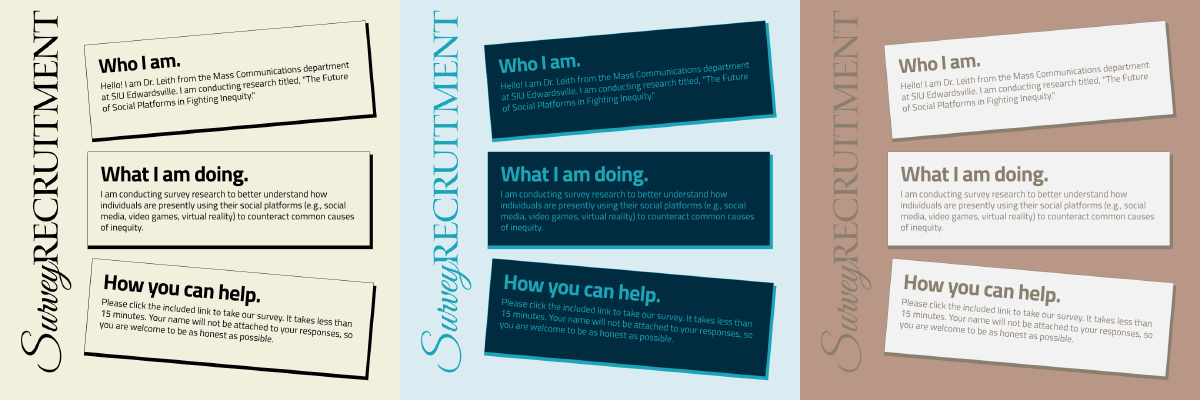
\includegraphics[width=1\linewidth,height=\textheight,keepaspectratio]{images/recruit-ad.png}
\caption{Instagram recruitment examples made with Adobe Express.}
\end{figure}

The recruitment materials should provide an overview of the study, including the study's title, the nature of the research, and the specific requirements for participants (IRB Recruitment Document, 2023). This includes detailing the time commitment required, the type of involvement (e.g., survey, interview), and the confidentiality measures that will be taken to protect participants' identities. The language used in these materials must be accessible, avoiding technical jargon to ensure that potential participants from diverse backgrounds can understand the content.

Moreover, the recruitment materials must emphasize the voluntary nature of participation. This is crucial in ensuring that individuals are not pressured to participate in the study. According to SIUE's IRB guidelines, participants must be informed that they can withdraw from the study at any time without facing any consequences (2023IRB-Research-Participant-Notification, 2023). These materials should also provide clear instructions on expressing interest in participating, such as contact details or survey links, ensuring the process is straightforward and respectful of the participants' time.

\subsection*{Developing Survey or Interview Questions}\label{developing-survey-or-interview-questions}
\addcontentsline{toc}{subsection}{Developing Survey or Interview Questions}

Survey and interview questions are fundamental components of research data collection, requiring careful design to ensure they effectively gather the necessary information while minimizing bias. At SIUE, the development of these questions must align with IRB protocols, particularly regarding their clarity, neutrality, and relevance to the research objectives.

The survey or interview questions should be constructed to elicit clear, honest responses, avoiding leading or loaded questions that might influence participants' answers. Questions should be directly related to the research objectives and structured logically to facilitate smooth progression through the survey or interview (IRB Protocol Guidance, 2023). It is also important to consider the cultural and contextual appropriateness of the questions, ensuring that they are sensitive to the participants' backgrounds and experiences.

\begin{figure}
\centering
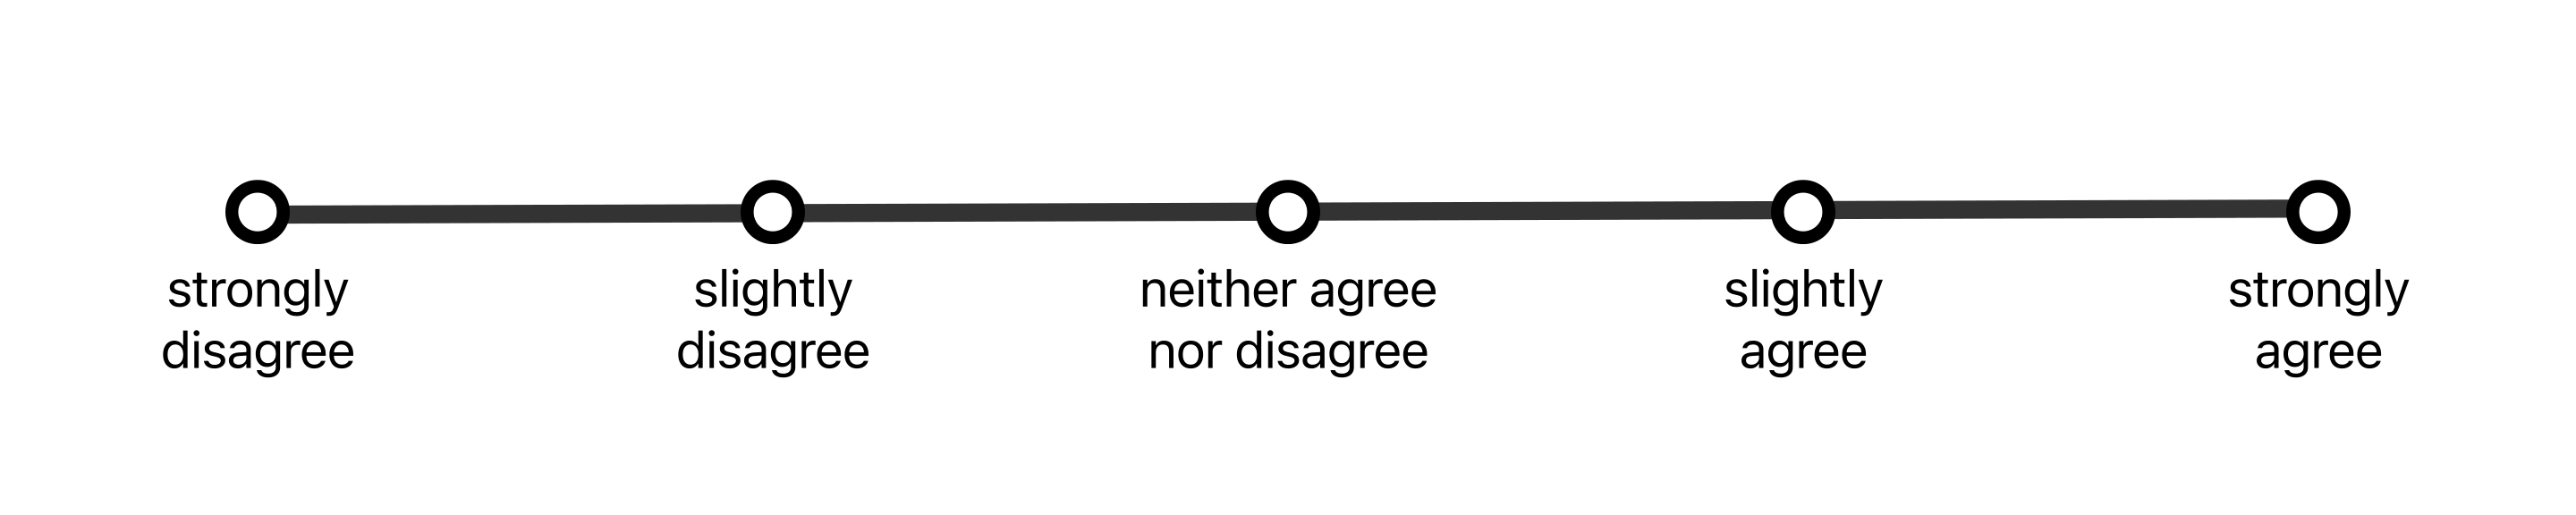
\includegraphics[width=1\linewidth,height=\textheight,keepaspectratio]{images/likert-scale.png}
\caption{Common Likert-type scale responses.}
\end{figure}

In addition, the IRB protocol requires that questions be framed to respect participants' confidentiality and anonymity. For instance, demographic questions should be designed to collect necessary information without compromising participants' identities. This might involve using broader categories for responses or providing options for participants to decline to answer specific questions (Protocols, 2024). Furthermore, the survey or interview process must include clear instructions on how data will be recorded and stored and the steps that will be taken to protect the data from unauthorized access.

\subsection*{The Debriefing Process}\label{the-debriefing-process}
\addcontentsline{toc}{subsection}{The Debriefing Process}

\textbf{Debriefing} is another crucial aspect of the IRB process, particularly in studies where deception is used or where participants might not be fully aware of the study's purpose during their involvement. Debriefing involves providing participants with a complete explanation of the study after their participation, ensuring they leave with a clear understanding of what the research was about and why certain methodologies, such as deception, were employed.

At SIUE, debriefing is especially important in research that involves sensitive topics or procedures that could cause distress. The debriefing process should be conducted in a manner that is sensitive to the participants' experiences during the study. It should include a thorough explanation of the study's true purpose, an overview of the participant's role, and an opportunity for participants to ask questions or express concerns. Additionally, researchers must provide contact information for follow-up questions and offer resources if the study touches on potentially distressing issues.

The \textbf{Research Participant Notification} document is a key tool in this process. It provides participants with formal documentation about the study, their rights, and contact information for any follow-up questions (Research Participant Notification, 2023). Researchers must ensure that this document is provided and explained to participants during the debriefing session.

\subsection*{Assessing and Minimizing Harm}\label{assessing-and-minimizing-harm}
\addcontentsline{toc}{subsection}{Assessing and Minimizing Harm}

\textbf{Assessing potential harm} to participants is a fundamental responsibility when navigating the IRB process. Harm can manifest in various forms, including physical discomfort, psychological distress, or social risks such as breaches of confidentiality. The IRB at SIUE requires that researchers conduct a thorough risk assessment as part of their protocol submission, outlining any potential risks and the measures that will be taken to mitigate them.

When assessing harm, researchers must consider both the likelihood and the severity of potential risks. For instance, a study involving interviews about traumatic experiences must account for the psychological impact of recalling such events on participants. The protocol must detail how these risks will be minimized, such as providing access to counseling services or designing interview questions sensitive to the participant's emotional state.

The \textbf{Protocols} document highlights the importance of a detailed risk-benefit analysis, where researchers must justify that the potential benefits of the research outweigh any identified risks (Protocols, 2024). This analysis is crucial for IRB approval, as the board will scrutinize whether the proposed protections are sufficient and appropriate given the nature of the study.

\subsection*{Offering Incentives}\label{offering-incentives}
\addcontentsline{toc}{subsection}{Offering Incentives}

\textbf{Incentives} can significantly influence participant recruitment and retention, but they must be carefully managed to avoid coercion. The IRB at SIUE requires that any incentives offered to participants be proportional to the time and effort required and not so large that they unduly influence participation, especially in studies involving any level of risk.

Incentives should be described in the IRB protocol submission, with a clear justification of why the chosen incentive is appropriate. For example, offering a small gift card or a modest monetary payment is generally acceptable, but offering a large sum of money might be considered coercive, particularly in studies involving vulnerable populations. The \textbf{IRB Protocol Guidance} document advises researchers to carefully consider the ethical implications of incentives and ensure that they do not overshadow the voluntary nature of participation (IRB Protocol Guidance, 2023).

\begin{figure}
\centering
\pandocbounded{
\includegraphics[keepaspectratio]{images/fig01e.jpg}}
\caption{An example of an excessive cash incentive}
\end{figure}

The \textbf{Recruitment Document} provided by SIUE is a template for informing potential participants about the study and any incentives they might receive (IRB Recruitment Document, 2023). It is essential to update this document with specific details relevant to your study and ensure that the incentives are described transparently.

\subsection*{Submission and Review Protocols}\label{submission-and-review-protocols}
\addcontentsline{toc}{subsection}{Submission and Review Protocols}

Navigating the IRB process at SIUE requires careful attention to detail in the submission and review stages. The IRB submission protocol involves several key steps, beginning with completing the IRB application in the Kuali system. Researchers must ensure that all protocol sections are thoroughly completed, including detailed descriptions of the research methods, participant recruitment strategies, and data management plans.

The \textbf{Protocols} document emphasizes the importance of thoroughly reading and responding to each question in the IRB submission, as incomplete or vague answers can lead to delays in the review process (Protocols, 2024). Researchers are encouraged to submit their protocols well before the anticipated start date to allow sufficient time for review and any necessary revisions.

Additionally, all student-led research at SIUE requires a faculty advisor's approval and signature, confirming that the student understands the ethical guidelines and that the study is methodologically sound (Faculty Advisor Signature, 2024). This step is crucial for ensuring that the research meets the university's standards and all ethical requirements.

Depending on the study's nature, the IRB review can fall into different categories, such as exempt, expedited, or full board review. Each category has specific requirements and timelines, and researchers must select the appropriate category based on their study's characteristics. The \textbf{IRB Protocol Guidance} document provides detailed instructions on determining the correct review category and what each entails (IRB Protocol Guidance, 2023).

\section{Ethical Considerations Specific to Mass Media Research}\label{ethical-considerations-specific-to-mass-media-research}

When conducting research in mass media, researchers must navigate unique ethical considerations arising from this field's specific nature. Unlike other disciplines, mass media research often involves observing and interacting with individuals in their natural environments, such as during their routine media consumption or within online communities. This approach brings forth specific challenges, particularly related to the \textbf{observer effect} and the role of the \textbf{observer-as-participant}. These concepts are crucial for understanding the potential influence a researcher can have on the subjects being studied and ensuring the research process's ethical integrity.

\subsection*{The Observer Effect}\label{the-observer-effect}
\addcontentsline{toc}{subsection}{The Observer Effect}

The \textbf{observer effect} refers to the phenomenon where the mere presence of a researcher can alter the behavior of the individuals being observed. This effect is particularly significant in mass media research, where participants' media consumption habits or online activities might change if they are aware of being monitored. For example, suppose individuals know their social media activity is under observation. In that case, they may modify their behavior by avoiding controversial content or engaging more carefully in discussions, leading to results that do not accurately reflect their typical behavior.

The observer effect presents a considerable challenge for researchers aiming to capture authentic data. Suppose the participants alter their behavior due to the awareness of being observed. In that case, the data collected may be skewed, leading to conclusions that are not genuinely representative of the subject's usual actions. This can compromise the validity of the research, making it difficult to draw accurate conclusions about media consumption patterns, audience behavior, or the effects of media content.

To mitigate the observer effect, researchers can employ \textbf{unobtrusive measures}---techniques that allow data collection without directly interacting with or influencing the subjects. For instance, researchers might analyze publicly available online data where participants are unaware of the specific focus of the study. However, this approach must be balanced with ethical considerations, particularly regarding the privacy of individuals and the potential implications of observing people without their explicit consent. Even when using unobtrusive measures, researchers must remain vigilant about the ethical implications, especially when dealing with sensitive topics or vulnerable populations.

\subsection*{The Observer-as-Participant Role}\label{the-observer-as-participant-role}
\addcontentsline{toc}{subsection}{The Observer-as-Participant Role}

Another critical concept in mass media research is the \textbf{observer-as-participant role}, in which the researcher not only observes the subjects but also actively engages with them. This dual role can provide valuable insights by allowing the researcher to experience the environment from within, gaining a deeper understanding of the social dynamics, cultural norms, and interactions that influence media consumption and behavior.

For example, a researcher studying online communities might participate in discussions, share content, and interact with community members to better understand how these interactions shape media consumption patterns and influence group behavior. This approach can offer a rich, nuanced perspective that is difficult to achieve through observation alone.

\begin{figure}
\centering
\pandocbounded{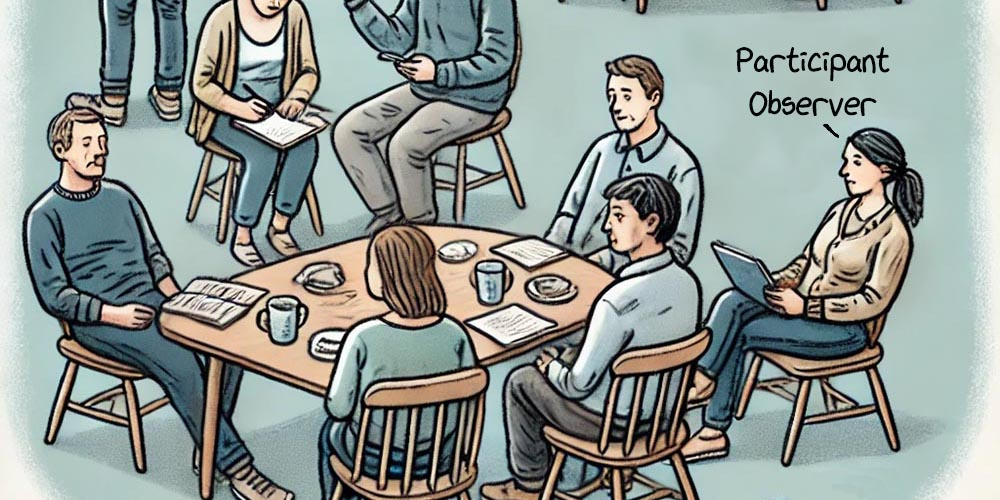
\includegraphics[keepaspectratio]{images/fig01f.jpg}}
\caption{Representation of participant observer}
\end{figure}

However, the observer-as-participant role also introduces significant ethical challenges. The researcher's involvement in the community can influence the behavior they aim to study, potentially leading to biased results. Moreover, there is the risk of compromising objectivity, as the researcher becomes part of the social fabric they study. Transparency is crucial in this role; researchers must disclose their identity and purpose to the subjects, ensuring that their interactions do not mislead or manipulate the community. Ethical dilemmas can arise if the researcher's participation changes the group dynamics or if their influence leads to outcomes that would not have occurred naturally.

Maintaining a balance between active participation and objective observation is essential but challenging. Researchers must constantly reflect on their role and the potential impact of their actions, taking care not to distort the data or influence the subjects more than necessary. In some cases, researchers may need to withdraw from active participation to ensure their presence does not overly affect the subjects' behavior.

\subsection*{Ethical Considerations and Strategies for Mitigation}\label{ethical-considerations-and-strategies-for-mitigation}
\addcontentsline{toc}{subsection}{Ethical Considerations and Strategies for Mitigation}

The observer effect and the observer-as-participant role highlight the ethical complexities of mass media research. Researchers must consider how their presence and actions might influence the subjects and the collected data. To address these challenges, several strategies can be employed:

\begin{enumerate}
\def\labelenumi{\arabic{enumi}.}
\item
  \textbf{Transparency}: Being transparent with participants about the research objectives and the researcher's role can help mitigate ethical concerns. This includes clear communication about the nature of the study, the role of the researcher, and how data will be collected and used.
\item
  \textbf{Informed Consent}: When feasible, obtaining informed consent from participants is crucial, particularly when the research involves direct interaction or observation. This ensures that participants are aware of the study and have agreed to participate in it, which can help mitigate the observer effect.
\item
  \textbf{Minimizing Interaction}: In cases where the observer effect might significantly alter participant behavior, researchers should consider minimizing their interaction with the subjects. This can be achieved through passive observation, anonymized data, or relying on existing data sets that do not involve real-time interaction.
\item
  \textbf{Ethical Reflection}: Researchers must engage in continuous ethical reflection, considering the potential impacts of their research on the subjects and the community. This involves evaluating the risks and benefits of the research, seeking advice from ethical review boards, and being prepared to adjust the research approach if ethical concerns arise.
\item
  \textbf{Balancing Roles}: When adopting the observer-as-participant role, researchers should carefully balance their involvement with the need to maintain objectivity. This might involve setting clear boundaries for participation and regularly reviewing the impact of their presence on the group dynamics.
\end{enumerate}

\chapter{Introduction to Research Papers}\label{introduction-to-research-papers}

\section{What are Research Papers}\label{what-are-research-papers}

Research papers, often referred to as scholarly articles, serve as vital conduits for disseminating original research findings, theoretical explorations, or critical analyses within the academic community. These documents are integral to the advancement of knowledge in various disciplines, providing a formalized medium through which researchers communicate their contributions to the broader academic and professional audience. Research papers are typically published in reputable academic journals, which are often associated with professional organizations or academic institutions. These journals serve as repositories of knowledge, where scholars can access and build upon the work of others, fostering the cumulative growth of knowledge in their respective fields.

\subsection*{Originality}\label{originality}
\addcontentsline{toc}{subsection}{Originality}

Originality is a fundamental criterion that distinguishes a research paper from other forms of academic writing. In the context of research, originality refers to the introduction of novel ideas, methods, or interpretations that have not been previously explored or sufficiently addressed within the existing body of literature. The originality of a research paper can be manifested through the identification of a unique research question or problem, the development of an innovative methodological approach, or the provision of fresh empirical evidence that challenges or refines established theories. This originality is not merely about being new for the sake of novelty; it must be significant and relevant, offering meaningful contributions to the academic field. An original research paper often fills a gap in the literature, addresses an overlooked aspect of a known issue, or provides new insights that lead to further research inquiries.

\subsection*{Methodology}\label{methodology}
\addcontentsline{toc}{subsection}{Methodology}

Methodology in a research paper is more than just a set of procedures; it is the backbone of the research that ensures the study's validity, reliability, and replicability. A well-defined methodology provides a clear roadmap for how the research was conducted, including the selection of participants or data sources, the tools and techniques used for data collection, and the methods of analysis. The methodology should be meticulously documented so that other researchers can critically assess the study's rigor and potentially replicate the findings in different contexts or with different samples. Moreover, a robust methodology reflects an understanding of the methodological challenges inherent to the research question and demonstrates the researcher's ability to address these challenges in a scientifically sound manner. The methodology section is where the researcher defends their choice of methods and discusses their limitations, providing a transparent account of the research process.

\subsection*{Evidence-Based}\label{evidence-based}
\addcontentsline{toc}{subsection}{Evidence-Based}

An evidence-based research paper is grounded in the systematic collection and analysis of data, which serves as the foundation for the paper's arguments and conclusions. The evidence presented can take many forms, including quantitative data from experiments or surveys, qualitative data from interviews or observations, or secondary data from existing literature. Regardless of the type of evidence, the key is that it must be relevant, reliable, and sufficient to support the research claims. Researchers must critically evaluate the evidence they collect, using appropriate analytical techniques to draw valid inferences. This process includes acknowledging any potential biases or limitations in the data, ensuring that the evidence is presented transparently and interpreted accurately. An evidence-based approach not only strengthens the credibility of the research findings but also aligns the study with the broader principles of scientific inquiry, where conclusions are drawn based on observable and verifiable facts rather than conjecture.

\subsection*{Peer Review}\label{peer-review}
\addcontentsline{toc}{subsection}{Peer Review}

Peer review is an essential component of the scholarly publication process, serving as a quality control mechanism that upholds the standards of academic integrity. During peer review, a research paper is scrutinized by independent experts in the relevant field who evaluate the paper's methodological soundness, the originality of its contributions, and the significance of its findings. The peer reviewers assess whether the research question is well-defined, whether the methodology is appropriate and rigorously applied, and whether the conclusions are adequately supported by the evidence. This process often involves multiple rounds of feedback, where the author is required to address reviewers' comments and make necessary revisions. The objective of peer review is to ensure that the research is robust, credible, and worthy of publication, thus contributing to the advancement of knowledge in the field. The peer review process also provides an opportunity for the author to refine their work based on expert feedback, enhancing the overall quality and impact of the research.

\subsection*{Structure}\label{structure}
\addcontentsline{toc}{subsection}{Structure}

The structure of a research paper is designed to facilitate the clear and logical presentation of the research process and findings. A typical research paper is organized into several key sections: the abstract, introduction, literature review, methodology, results, discussion, and references. Each section serves a distinct purpose in the overall narrative of the paper. The abstract offers a brief summary of the research, providing readers with an overview of the study's objectives, methods, and key findings. The introduction establishes the research context, presenting the research question and its significance while reviewing relevant literature to position the study within the existing body of knowledge. The methodology section details the research design and methods used, allowing for transparency and reproducibility. The results section presents the findings, often with the aid of tables, figures, or other visual aids. The discussion interprets these findings, exploring their implications, limitations, and potential for future research. Finally, the references section cites all the sources used, ensuring proper attribution and enabling readers to locate the original sources for further investigation. This structured approach not only enhances the clarity and coherence of the paper but also ensures that it meets the rigorous standards of academic writing.

\section{How to Find Research Papers}\label{find}

Finding research papers is an essential skill for students and researchers alike. Research papers are the backbone of academic work, providing the evidence, insights, and foundations necessary for developing new theories, testing hypotheses, and building knowledge. Whether you're writing a paper, preparing a presentation, or simply expanding your understanding of a topic, knowing how to locate and access research papers efficiently is crucial. Below are some effective strategies to help you find the research papers you need.

\subsection*{Check Your University Library}\label{check-your-university-library}
\addcontentsline{toc}{subsection}{Check Your University Library}

Your university library is one of the most valuable resources for finding research papers. University libraries provide access to a vast array of academic materials, including books, journals, and databases that are often not available for free online. Here's how to make the most of your university library's resources:

\href{https://www.siue.edu/lovejoy-library/ask-a-librarian/}{\textbf{Talk to a Librarian}}\textbf{.} Librarians are highly trained in information retrieval and can assist you in finding the most relevant and high-quality research papers for your topic. They can guide you to the right databases, help you refine your search strategies, and even suggest keywords or subject headings you might not have considered. Many libraries also offer personalized research consultations where you can get in-depth assistance on your specific research needs.

\href{https://i-share-sie.primo.exlibrisgroup.com/discovery/search?vid=01CARLI_SIE:CARLI_SIE&lang=en}{\textbf{Use the Library's Online Catalog}}\textbf{.} The online catalog is a powerful tool that allows you to search the entire collection of your university library, including books, journals, e-books, and other materials. You can narrow down your results by using specific search terms or filters to find the most relevant research papers. Most catalogs also allow you to see whether the materials are available physically in the library or online.

\href{https://libguides.siue.edu/az.php}{\textbf{Access the Library's Databases}}\textbf{.} University libraries subscribe to many academic databases that provide access to thousands of scholarly journals, articles, and other resources. These databases are often organized by subject, making finding research papers in your field of study easier. Popular databases include JSTOR, ProQuest, and EBSCOhost, among others. Databases can usually be searched by keyword, author, or subject, and many offer advanced search options that allow you to combine terms and apply filters to get the best results.

\subsection*{Use a specialized search engine.}\label{use-a-specialized-search-engine.}
\addcontentsline{toc}{subsection}{Use a specialized search engine.}

Specialized search engines are designed to search for specific types of information, such as research articles. Here are some tips on how to use a specialized search engine to find research articles:

\subsubsection*{Where to Search}\label{where-to-search}
\addcontentsline{toc}{subsubsection}{Where to Search}

When searching for research articles, knowing where to search is just as important as how you search. Specialized search engines are designed specifically for academic and scholarly materials, making them ideal tools for finding high-quality research papers. Unlike general search engines like Google, these specialized tools index scholarly content such as journal articles, conference papers, and theses. Below are some key specialized search engines and tips on how to choose the right one for your research needs.

Selecting the appropriate search engine depends on your research topic. If you're studying medicine or biology, PubMed should be your first choice. For engineering and technology, IEEE Xplore and ACM Digital Library are more suitable. If your research spans multiple disciplines, starting with Google Scholar, Web of Science, or Scopus may yield the broadest results.

\textbf{1. Google Scholar}

Google Scholar is one of the most widely used academic search engines. It provides access to a broad range of scholarly articles, theses, books, conference papers, and patents across various disciplines. It's a good starting point for most research topics due to its extensive coverage.

\href{https://scholar.google.com/}{
\includegraphics[width=1\linewidth,height=\textheight,keepaspectratio]{images/google-scholar.jpg}}

\textbf{2. PubMed}

PubMed is the go-to search engine for research in the biomedical and life sciences. It offers a comprehensive collection of articles from journals in medicine, biology, and health-related fields. If your research is in these areas, PubMed is an indispensable resource.

\href{https://pubmed.ncbi.nlm.nih.gov/}{
\includegraphics[width=1\linewidth,height=\textheight,keepaspectratio]{images/pubmed.jpg}}

\textbf{3. Web of Science}

Web of Science is a powerful tool that covers a wide array of disciplines, including the sciences, social sciences, arts, and humanities. It is particularly useful for citation tracking, allowing you to see how often an article has been cited by others, which can help you gauge its impact and relevance.

\href{https://go.openathens.net/redirector/siue.edu?url=https\%3A\%2F\%2Fwebofknowledge.com\%2FWOS}{
\includegraphics[width=1\linewidth,height=\textheight,keepaspectratio]{images/web-of-science.jpg}}

\textbf{4. Scopus}

Scopus is another multidisciplinary database, with an extensive collection of articles in the sciences, technology, medicine, social sciences, and more. Scopus also provides citation analysis, making it useful for understanding the influence of a particular study within its field.

\href{https://www.scopus.com/home.uri}{
\includegraphics[width=1\linewidth,height=\textheight,keepaspectratio]{images/scopus.jpg}}

\textbf{5. IEEE Xplore}

IEEE Xplore is the premier search engine for research in electrical engineering, computer science, and electronics. It indexes a vast number of conference papers, journal articles, and standards published by the IEEE.

\href{https://ieeexplore.ieee.org/Xplore/home.jsp}{
\includegraphics[width=1\linewidth,height=\textheight,keepaspectratio]{images/ieee-xplore.jpg}}

\textbf{6. ACM Digital Library}

The ACM Digital Library is essential for computer science research, offering a wide range of articles, conference proceedings, and other publications by the Association for Computing Machinery. It is particularly valuable for topics in software engineering, computer systems, and human-computer interaction.

\href{https://dl.acm.org/}{
\includegraphics[width=1\linewidth,height=\textheight,keepaspectratio]{images/acm-digital-library.jpg}}

\subsubsection*{How to Search}\label{how-to-search}
\addcontentsline{toc}{subsubsection}{How to Search}

Once you've chosen where to search, understanding how to effectively use these tools is crucial for finding the most relevant and high-quality research articles. Below are strategies to help you optimize your search process.

\textbf{1. Use Keywords Effectively}

Keywords are the foundation of any search. Start by identifying the main concepts of your research topic. For example, if you're researching the effects of social media on mental health, your main keywords might be ``social media,'' ``mental health,'' and ``impact.'' Input these keywords into your chosen search engine to begin your search.

\textbf{2. Utilize Advanced Search Features}

Most specialized search engines offer advanced search options that allow you to refine your search. You can often specify criteria such as:

\begin{itemize}
\tightlist
\item
  \textbf{Publication Date:} Limit your results to recent publications to ensure the information is up-to-date.
\item
  \textbf{Language:} If you're only interested in articles written in a specific language, you can filter results accordingly.
\item
  \textbf{Document Type:} Narrow down your search to only include journal articles, reviews, conference papers, etc.
\end{itemize}

For instance, in Google Scholar, you can access these options by clicking on ``Advanced Search,'' which allows you to combine keywords with Boolean operators, search within specific journals, or exclude certain terms from your results.

\textbf{3. Use Quotation Marks for Exact Phrases}

When searching for specific phrases, using quotation marks can help ensure that the search engine looks for the words together in the exact order you've specified. For example, searching for ``impact of social media on mental health'' will return results where this phrase appears as is, rather than finding articles where these words appear separately.

\textbf{4. Apply Boolean Operators}

Boolean operators (AND, OR, NOT) are powerful tools for refining your search:

\begin{itemize}
\tightlist
\item
  \textbf{AND:} Use AND to narrow your search. For example, ``social media AND mental health'' will return articles that contain both terms.
\item
  \textbf{OR:} Use OR to broaden your search by including synonyms or related terms. For example, ``social media OR social networks'' will return articles that include either term.
\item
  \textbf{NOT:} Use NOT to exclude unwanted terms. For example, ``social media NOT Facebook'' will exclude articles that specifically focus on Facebook.
\end{itemize}

\begin{figure}
\centering
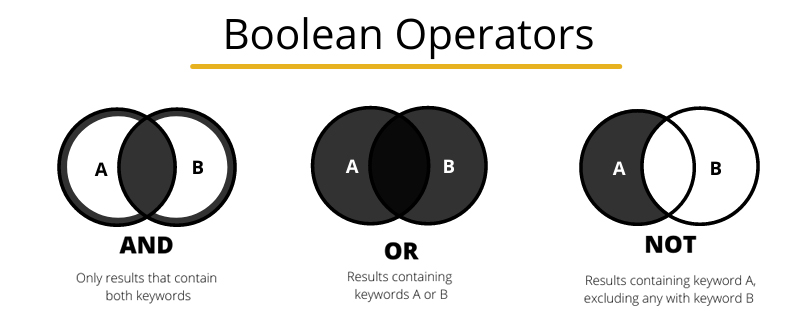
\includegraphics[width=1\linewidth,height=\textheight,keepaspectratio]{images/boolean.jpg}
\caption{Boolean Operators}
\end{figure}

\textbf{5. Read and Evaluate Search Results Carefully}

After conducting your search, take the time to review the results carefully. Pay attention to the title, abstract, and keywords of each article to determine its relevance to your research. Ensure that the articles are published in reputable journals, have undergone peer review, and are authored by credible experts in the field.

\textbf{6. Use Filters to Narrow Down Results}

Many specialized search engines provide filters that allow you to narrow down results by various criteria, such as year of publication, subject area, or type of document. For instance, if you are looking for the most recent studies on a topic, you can filter your search results to only include articles published in the last five years.

\textbf{7. Refer to Help Documentation}

If you're unfamiliar with a particular search engine, refer to its help documentation. These guides often include tips on using advanced search features, understanding search results, and optimizing your search queries. For example, Google Scholar's help page provides explanations on how to refine searches, save citations, and set up alerts for new research.

By combining the right search engine with effective search strategies, you can efficiently find the research articles you need for your academic work.

\subsection*{Using Social Media to Find Research Articles}\label{using-social-media-to-find-research-articles}
\addcontentsline{toc}{subsection}{Using Social Media to Find Research Articles}

Social media has become a powerful tool for academics and researchers, providing a platform to share, discover, and discuss research articles. By leveraging the features of various social media platforms, you can stay informed about the latest developments in your field, find relevant research articles, and connect with other scholars. Below are some effective strategies for using social media to find research articles.

\subsubsection*{1. Follow Researchers and Research Institutions}\label{follow-researchers-and-research-institutions}
\addcontentsline{toc}{subsubsection}{1. Follow Researchers and Research Institutions}

One of the most direct ways to stay updated with the latest research is by following individual researchers, academic institutions, and research organizations on social media. Many scholars use platforms like Twitter, LinkedIn, and ResearchGate to share their latest publications, conference presentations, and ongoing projects. By following these accounts, you can receive updates on new research articles as soon as they are published. Additionally, institutions often share open access articles, preprints, and links to publications that might be behind paywalls elsewhere, providing valuable resources for your own research.

\begin{itemize}
\tightlist
\item
  \textbf{Tip:} When following researchers, consider looking at their followers and who they follow as well. This can help you find other relevant scholars and institutions in your area of interest.
\end{itemize}

\subsubsection*{2. Use Relevant Hashtags}\label{use-relevant-hashtags}
\addcontentsline{toc}{subsubsection}{2. Use Relevant Hashtags}

Hashtags on social media platforms like Twitter and Instagram serve as powerful tools for categorizing content and making it discoverable to a broader audience. Researchers and institutions often use specific hashtags related to their field, research topic, or academic events. By searching for or following these hashtags, you can easily find posts related to recent research articles, discussions on emerging trends, and links to relevant studies.

\begin{itemize}
\tightlist
\item
  \textbf{Example:} Searching for hashtags such as \#OpenAccess, \#ScienceTwitter, \#AcademicChatter, or discipline-specific tags like \#PsychResearch or \#ClimateScience can lead you to valuable research articles and academic discussions.
\end{itemize}

\subsubsection*{3. Join Research Groups and Communities}\label{join-research-groups-and-communities}
\addcontentsline{toc}{subsubsection}{3. Join Research Groups and Communities}

Social media platforms host numerous groups and communities dedicated to specific research fields or interdisciplinary topics. These groups, which can be found on platforms like Facebook, LinkedIn, and Reddit, are spaces where researchers share their work, seek advice, and discuss recent findings. Joining these groups allows you to engage with peers, discover articles that might not be widely publicized, and gain insights from ongoing academic discussions.

\begin{itemize}
\tightlist
\item
  \textbf{Tip:} When joining a group, take the time to introduce yourself and share your research interests. Active participation can lead to more meaningful connections and opportunities to find relevant research articles.
\end{itemize}

\subsubsection*{4. Attend Online Conferences and Workshops}\label{attend-online-conferences-and-workshops}
\addcontentsline{toc}{subsubsection}{4. Attend Online Conferences and Workshops}

The shift to virtual events has made it easier than ever to attend academic conferences and workshops from anywhere in the world. These events are often live-streamed on social media platforms or have dedicated hashtags for participants to follow along and discuss. Attending these online events allows you to access presentations, papers, and discussions that are directly relevant to your research. Additionally, many conferences post recordings of sessions or provide access to conference papers after the event, giving you further opportunities to explore new research.

\begin{itemize}
\tightlist
\item
  \textbf{Tip:} After attending a session, engage with the speakers and attendees on social media by sharing your thoughts or asking questions. This can help you build a network of contacts who may share additional resources or research articles.
\end{itemize}

\subsubsection*{Specific Social Media Platforms to Use}\label{specific-social-media-platforms-to-use}
\addcontentsline{toc}{subsubsection}{Specific Social Media Platforms to Use}

\textbf{Twitter:} Twitter is an excellent platform for real-time research updates, especially by following researchers and journals and using hashtags. Many academic communities thrive on Twitter, making it a rich resource for finding the latest studies.

\textbf{LinkedIn:} LinkedIn is ideal for connecting with professionals and academics in your field. Researchers often share their publications and discuss their implications on LinkedIn, making it a valuable platform for professional networking and discovering research articles.

\textbf{ResearchGate:} ResearchGate is a dedicated social networking site for researchers. It allows you to follow researchers, access their publications, request full-text articles, and engage in discussions. It's particularly useful for finding peer-reviewed research and collaborating with other scholars.

\textbf{Evaluating Sources on Social Media}

While social media is a powerful tool for discovering research articles, it is crucial to critically evaluate the sources you find. Not all articles shared on social media are of high quality or come from reputable journals. Always consider the credibility of the author, the publication venue, and the methodology of the research before incorporating it into your own work. If in doubt, consult a librarian or an academic advisor for further guidance.

\subsection*{Contacting Experts in Your Field}\label{contacting-experts-in-your-field}
\addcontentsline{toc}{subsection}{Contacting Experts in Your Field}

In addition to using social media, directly contacting experts in your field can be an invaluable way to find research articles and gain deeper insights into your study area. Experts can provide recommendations for key papers, suggest emerging research areas, and even share unpublished work that may not yet be available in databases.

\subsubsection*{1. Talk to Your Professors or Advisors}\label{talk-to-your-professors-or-advisors}
\addcontentsline{toc}{subsubsection}{1. Talk to Your Professors or Advisors}

Your professors and academic advisors are often the best starting point when seeking expert guidance. They have deep knowledge of the field, are familiar with the latest research, and can point you toward seminal papers or recommend specific articles that are highly relevant to your research. Moreover, they may have access to articles or resources that are not available to students, which can further enrich your research.

\begin{itemize}
\tightlist
\item
  \textbf{Tip:} When approaching your professors, be specific about your research topic and what you hope to learn. This will help them provide more targeted recommendations.
\end{itemize}

\subsubsection*{2. Attend Conferences and Workshops}\label{attend-conferences-and-workshops}
\addcontentsline{toc}{subsubsection}{2. Attend Conferences and Workshops}

Conferences and workshops are excellent venues for meeting experts and learning about the latest research. These events often feature presentations from leading scholars, providing an opportunity to hear about their work directly. After a presentation, don't hesitate to approach the speaker with questions or requests for further reading. Many experts are happy to share their articles or direct you to where you can find them.

\begin{itemize}
\tightlist
\item
  \textbf{Tip:} Prepare a list of questions or topics of interest before attending a conference. This will help you maximize the networking opportunities and identify experts who can assist with your research.
\end{itemize}

\subsubsection*{3. Read Research Blogs and Newsletters}\label{read-research-blogs-and-newsletters}
\addcontentsline{toc}{subsubsection}{3. Read Research Blogs and Newsletters}

Many experts maintain blogs or contribute to newsletters that discuss their research and developments in the field. These platforms are often more accessible than academic journals and provide insights into the latest research trends. Following these blogs or subscribing to newsletters can keep you informed about new publications and give you a more nuanced understanding of ongoing debates in your field.

\begin{itemize}
\tightlist
\item
  \textbf{Tip:} Look for blogs that are peer-reviewed or written by recognized experts in the field to ensure the information is reliable.
\end{itemize}

\subsubsection*{4. Use Social Media to Connect with Experts}\label{use-social-media-to-connect-with-experts}
\addcontentsline{toc}{subsubsection}{4. Use Social Media to Connect with Experts}

As mentioned earlier, social media platforms are also useful for connecting with experts. By following researchers, engaging with their posts, and joining relevant groups, you can build relationships that may lead to further collaboration or recommendations for research articles. Many researchers are open to sharing their work or discussing their findings with interested peers, especially if you approach them respectfully and with clear questions.

\begin{itemize}
\tightlist
\item
  \textbf{Tip:} When reaching out to an expert on social media, always introduce yourself and explain why you are interested in their work. Be concise and professional in your communication to make a positive impression.
\end{itemize}

\subsubsection*{Finding and Contacting Experts}\label{finding-and-contacting-experts}
\addcontentsline{toc}{subsubsection}{Finding and Contacting Experts}

\textbf{Search by Name or Topic:} Use academic databases, professional organizations, or specialized directories to find experts in your field. You can search by specific research topics or by the names of researchers who have published influential work in your area of interest.

\textbf{Look for Published Authors:} Identify experts by looking at the authors of the research articles you find through databases like Google Scholar or Scopus. Those who frequently publish in reputable journals are likely to be well-established in their field.

\textbf{Seek Out Conference Presenters:} Experts who present at conferences are often leaders in their field. You can find information about upcoming conferences on the websites of professional organizations. After identifying relevant presenters, consider reaching out to them with specific questions or requests for further reading.

\textbf{Engage with Active Social Media Users:} Many researchers are active on platforms like Twitter, LinkedIn, and ResearchGate. By engaging with their content---whether through likes, comments, or direct messages---you can start a conversation that may lead to valuable research recommendations.

When contacting experts, be mindful of their time and make your requests clear and concise. Express gratitude for their assistance and follow up with any additional questions you may have after your initial conversation. Building a professional relationship with experts in your field can significantly enhance your research and provide you with insights that are not readily available through other means.

\section{How to Read Research Papers}\label{read}

There are many different approaches to reading a research paper, but these are some of the most effective ones.

\subsection*{The three-pass approach.}\label{the-three-pass-approach.}
\addcontentsline{toc}{subsection}{The three-pass approach.}

The three-pass approach to reading a research paper is a method of reading a paper in three stages, each with a specific goal.

\textbf{The first pass}. This is a quick scan to capture a high-level view of the paper. You should read the title, abstract, and introduction carefully, and then skim the rest of the paper, paying attention to the headings and subheadings. The goal of this pass is to get a general understanding of what the paper is about, its main points, and its contributions to the field.

\textbf{The second pass}: This is a more detailed reading of the paper. You should read the introduction and conclusion carefully, and then read the rest of the paper in more detail, paying attention to the methods, results, and discussion. The goal of this pass is to understand the paper's arguments and evidence, and to assess its strengths and weaknesses.

\textbf{The third pass}: This is a critical reading of the paper. You should read the paper carefully, taking notes and challenging the author's assumptions and conclusions. The goal of this pass is to fully understand the paper and to be able to critically evaluate its claims.

\subsection*{The question-based approach.}\label{the-question-based-approach.}
\addcontentsline{toc}{subsection}{The question-based approach.}

The question-based approach to reading a research paper is a method of reading a paper by asking questions about the paper as you read. This approach can help you to focus your reading and to ensure that you understand the key points of the paper.

Here are some questions that you can ask yourself as you read a research paper:

\begin{itemize}
\item
  What is the purpose of the paper?
\item
  What are the main questions that the paper addresses?
\item
  What are the key findings of the paper?
\item
  How does the paper contribute to the existing body of knowledge?
\item
  What are the strengths and weaknesses of the paper?
\item
  How does the paper relate to my own research interests?
\end{itemize}

You can also ask more specific questions that are relevant to the specific paper that you are reading. For example, if you are reading a paper about a new medical treatment, you might ask questions about the safety and effectiveness of the treatment.

The question-based approach can be used in conjunction with the three-pass approach to reading a research paper. In the first pass, you can ask general questions about the paper to get a sense of what it is about. In the second pass, you can ask more specific questions to understand the paper in more detail. In the third pass, you can critically evaluate the paper by asking questions about its methods, findings, and conclusions.

The question-based approach is a flexible method that can be adapted to your own needs and preferences. By asking questions as you read, you can improve your understanding of research papers and your ability to critically evaluate their claims. The question-based approach is a valuable tool for reading and understanding research papers. By asking questions as you read, you can improve your comprehension and critical thinking skills.

\subsection*{The active reading approach.}\label{the-active-reading-approach.}
\addcontentsline{toc}{subsection}{The active reading approach.}

Active reading is a method of reading that involves engaging with the text in a thoughtful and critical way. It is different from passive reading, which is simply reading the text without thinking about it.

Active reading can be used to read any type of text, but it is especially important for reading research papers. Research papers are often dense and technical, so it is important to be actively engaged in order to understand them.

Here are some tips for active reading:

\textbf{Ask questions}: As you read, ask yourself questions about the text. What is the author's purpose? What are the main points? What evidence does the author provide to support their claims?

\textbf{Take notes}: Taking notes can help you to remember the key points of the text and to track your progress. You can take notes in the margins of the text, or you can use a separate notebook.

\textbf{Summarize}: After each section of the text, summarize the key points in your own words. This will help you to solidify your understanding of the text.

\textbf{Discuss the text with others}: Talking to others about a text can help you to gain new insights and perspectives.

\textbf{Annotate the text}: Annotating the text means making notes and comments in the margins. This can help you to highlight important passages, ask questions, and make connections between different parts of the text.

\textbf{Use a highlighter}: Highlighting important passages can help you to focus your attention and to remember the key points of the text.

\textbf{Take a break}: Don't try to read a research paper in one sitting. Take breaks to refresh your mind and to come back to the text with fresh eyes.

Active reading takes time and effort, but it is a valuable skill for anyone who wants to learn and grow. By actively reading research papers, you can improve your comprehension, critical thinking skills, and ability to learn new things.

\subsection*{The collaborative reading approach.}\label{the-collaborative-reading-approach.}
\addcontentsline{toc}{subsection}{The collaborative reading approach.}

This approach involves reading the paper with a partner or group of people. This can be helpful for getting different perspectives on the paper and for identifying areas where you need clarification.

No matter which approach you choose, it is important to take your time and read the paper carefully. Research papers can be dense and challenging, but they can also be very rewarding. By taking the time to read them carefully, you can learn a lot about your field and contribute to the advancement of knowledge. The question-based approach is a valuable tool for reading and understanding research papers. By asking questions as you read, you can improve your comprehension and critical thinking skills.

\section{How to Write Research Papers}\label{write}

\subsection*{Sections of an Academic Paper}\label{sections-of-an-academic-paper}
\addcontentsline{toc}{subsection}{Sections of an Academic Paper}

Writing a research report involves meticulously organizing your work to clearly communicate the purpose, methods, findings, and conclusions of your study. Each section of the report is crucial, serving a specific function in guiding the reader through your research journey. Understanding how to craft each part effectively will help you produce a coherent, credible, and impactful report.

\subsubsection*{Title}\label{title}
\addcontentsline{toc}{subsubsection}{Title}

The title of your research report is more than just a label; it is the first impression that sets the stage for your entire study. A well-crafted title should be clear, concise, and informative, giving the reader a snapshot of the study's focus while also piquing their interest. Typically, a title should not exceed 12 words, striking a balance between being descriptive and concise. It should accurately reflect the main topic of the paper, using specific language that gives the reader a clear idea of what to expect. For instance, rather than using vague terms, the title should include specific variables or populations being studied. The formatting of the title is also important. It should be bold, centered, and double-spaced on the title page. Only the first word of the title and any proper nouns should be capitalized, even when using a semi-colon, where the word following it is treated as a new first word. This attention to detail in the title not only adheres to academic conventions but also conveys a sense of professionalism and precision, setting the tone for the rest of the report.

\subsubsection*{Abstract}\label{abstract}
\addcontentsline{toc}{subsubsection}{Abstract}

The abstract is one of the most critical components of a research report, serving as a concise summary that encapsulates the entire study. It typically ranges between 150 and 250 words and should be written in past tense. The abstract must efficiently convey the purpose of the study, the methods used, the main findings, and the conclusions drawn, providing readers with a clear overview of what the report entails. Since the abstract is often the first---and sometimes the only---part of the report that others will read, it needs to be clear and informative, free of jargon, and devoid of citations. Crafting a strong abstract involves striking a balance between brevity and completeness; it should cover the key aspects of the study without delving into unnecessary details. In learning to write effective abstracts, students will review examples from published research, which will highlight how successful abstracts succinctly summarize complex studies. Through writing exercises and peer reviews, students will develop the skill to distill their research into a compelling, accurate summary, while avoiding common pitfalls like vagueness or excessive detail that can obscure the main message.

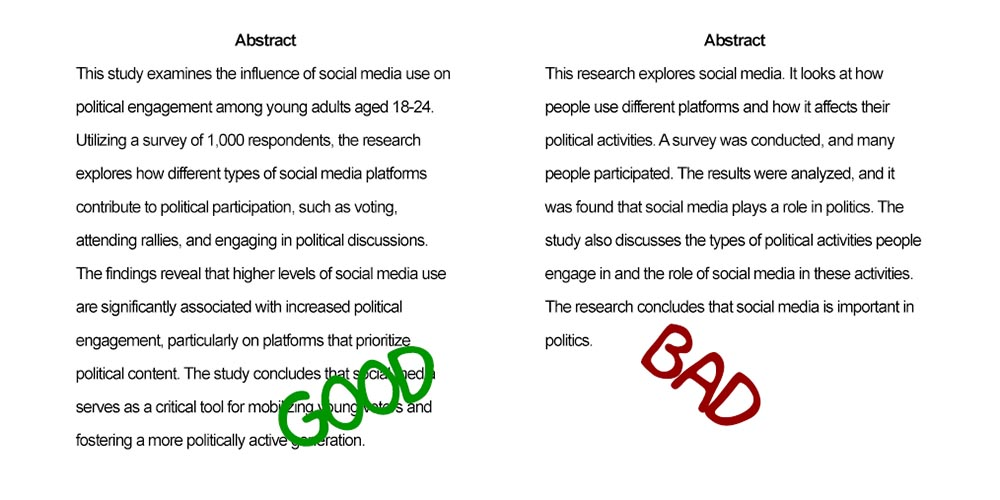
\includegraphics[width=1\linewidth,height=\textheight,keepaspectratio]{images/fig081.jpg}

\subsubsection*{Introduction}\label{introduction}
\addcontentsline{toc}{subsubsection}{Introduction}

The introduction of your research report serves as the gateway to your study, providing the necessary background information and framing the research problem within a broader context. A well-written introduction should clearly state the research problem, explain its significance, and outline the research question or hypothesis. This section is crucial for engaging the reader, as it not only introduces the topic but also justifies why the study is important. A strong introduction links the research question to existing literature or ongoing debates in the field, setting the stage for the subsequent sections of the report. In crafting an introduction, it is essential to balance providing enough background to understand the research with keeping the reader's interest. Students will examine examples from academic journals to see how effective introductions establish context, articulate the research problem, and lead seamlessly into the study's objectives. By practicing drafting introductions for hypothetical studies, students will learn to frame their research in a way that is both compelling and informative, ensuring that their readers are both engaged and well-informed from the outset.

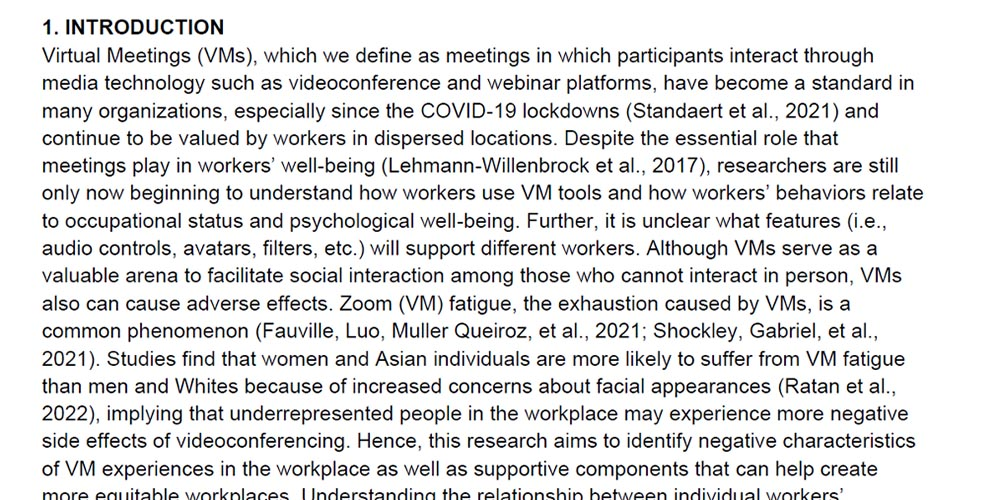
\includegraphics[width=1\linewidth,height=\textheight,keepaspectratio]{images/fig082.jpg}

\subsubsection*{Literature Review}\label{literature-review}
\addcontentsline{toc}{subsubsection}{Literature Review}

The literature review is a foundational component of a research report, serving as a synthesis of existing research that situates your study within the broader academic discourse. It is not merely a summary of related studies but a critical evaluation that identifies gaps in the literature, justifies the relevance of your research, and demonstrates your understanding of the field. A well-crafted literature review connects various studies, highlighting how they relate to your research question and setting the stage for your contribution to the field. This section requires a thorough review of existing literature, with a focus on synthesizing findings rather than simply cataloging them. To aid in the construction of a literature review, students will be provided with guidelines that emphasize the importance of critical evaluation and thematic organization. Writing exercises will involve summarizing and synthesizing research on a given topic, identifying key themes, and discussing how these themes relate to the research question. Through these exercises, students will learn to craft a literature review that not only provides context but also establishes a strong foundation for their study, leading naturally to the formulation of their research question.

\subsubsection*{Methods}\label{methods}
\addcontentsline{toc}{subsubsection}{Methods}

The methods section of a research report is where you detail how the research was conducted, providing a roadmap that allows others to replicate your study. This section should include a comprehensive description of the participants, materials, procedures, and methods of data analysis used in the study. Clarity and precision are crucial, as the goal is to provide enough detail for another researcher to replicate the study exactly. The methods section is typically written in the past tense, as it describes actions that have already been completed. To assist in writing this section, students will be provided with a template or checklist to ensure all necessary details are included. They will practice writing a method section based on a described experiment or survey, followed by class reviews to discuss completeness and clarity. These discussions will emphasize the importance of transparency in the methods section, as it underpins the study's scientific rigor and reliability. By mastering the methods section, students will be able to communicate the how of their research clearly and effectively, ensuring that their study can be trusted and potentially replicated by others in the field.

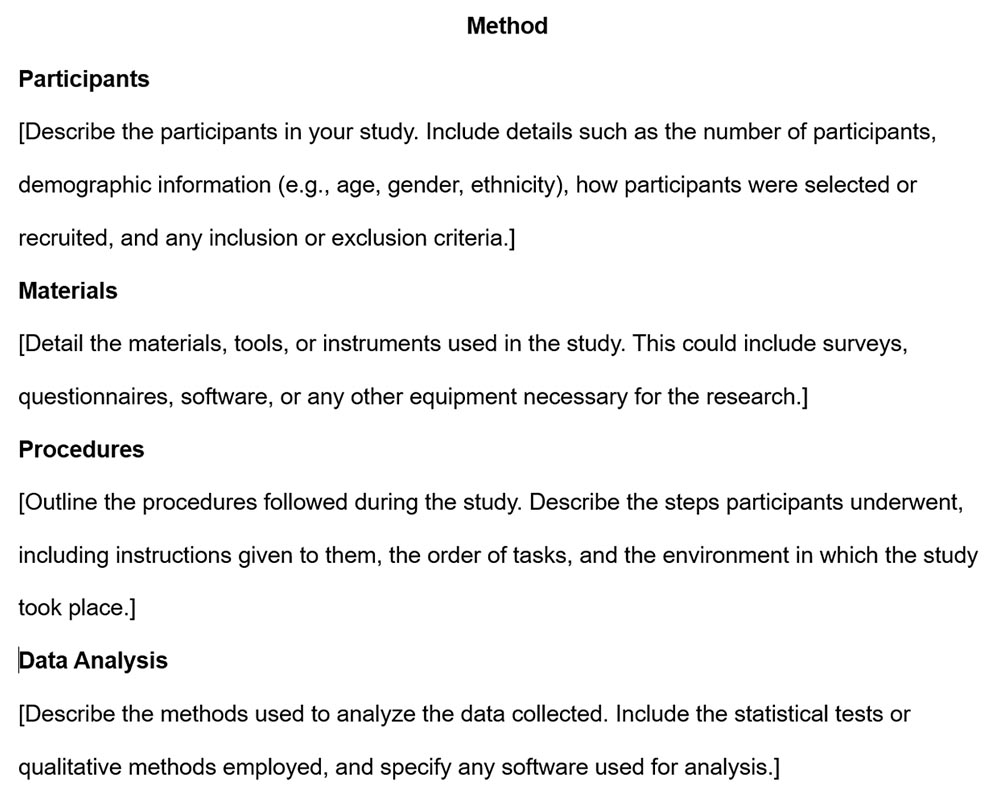
\includegraphics[width=1\linewidth,height=\textheight,keepaspectratio]{images/fig083.jpg}

\subsubsection*{Results}\label{results}
\addcontentsline{toc}{subsubsection}{Results}

The results section of a research report presents the findings of your study, providing the raw data and statistical analyses that support your conclusions. This section should be organized logically and clearly, with the data presented in a way that is easy to follow. Tables, graphs, and figures are often used to illustrate the data, making it more accessible to the reader. The results section should be objective and free of interpretation; its purpose is to present the facts as they are, allowing the data to speak for itself. In teaching how to write this section, students will learn to select the most appropriate methods for presenting their data, ensuring that it is both clear and comprehensive. Exercises will involve organizing data into tables and graphs and writing a results section based on these visual representations. By focusing on the clarity and objectivity required in the results section, students will develop the ability to present their findings in a manner that is both accurate and easy to interpret.

\subsubsection*{Discussion}\label{discussion}
\addcontentsline{toc}{subsubsection}{Discussion}

The discussion section is where you interpret the results of your study, relating them back to the research question and the existing literature. This section should provide a thoughtful analysis of what the results mean, how they contribute to the field, and what their implications are for future research. It is also where you discuss the limitations of your study and suggest directions for future research. The discussion section should be written in the present tense, as it deals with the implications of your findings. To help students write an effective discussion, they will be guided through examples that show how to connect the results to the literature review and research question, offering a critical analysis that goes beyond the data itself. Writing exercises will focus on developing a narrative that ties the findings to broader theoretical and practical implications, while also acknowledging the study's limitations. Through this process, students will learn to craft a discussion that is both insightful and grounded in the data, providing a clear interpretation of what their findings mean and why they matter.

\subsubsection*{References}\label{references}
\addcontentsline{toc}{subsubsection}{References}

The references section is where you list all the sources cited in your research report, providing full citations in the appropriate format (typically APA style). This section is essential for giving credit to the original authors and for allowing readers to locate the sources you used. Accurate and consistent referencing is crucial for maintaining the credibility of your research report. To familiarize students with APA formatting rules, they will be introduced to the APA Publication Manual and other online resources. A workshop will be conducted where students practice formatting references for various types of sources, such as books, journal articles, and websites. During this workshop, common citation errors will be discussed, along with strategies to avoid them. The emphasis will be on maintaining consistency and accuracy in references, as these are key to producing a credible and professional research report.

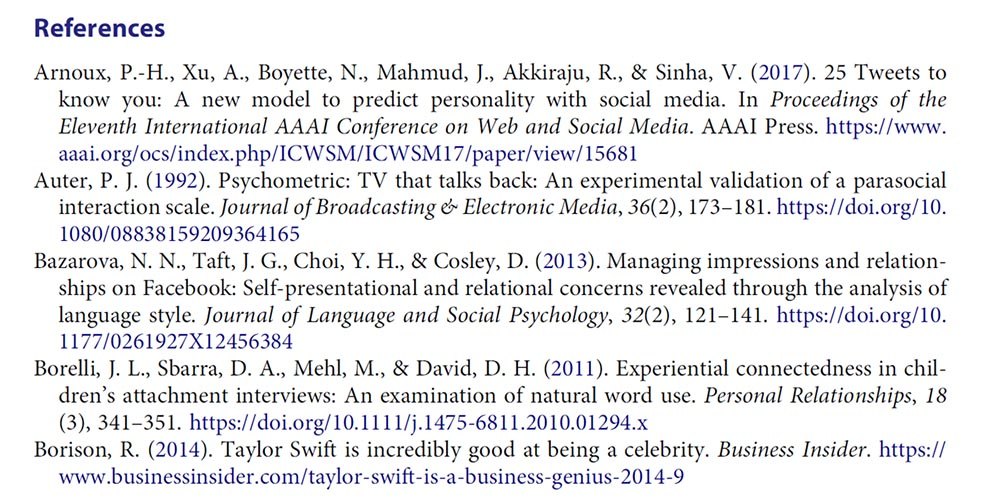
\includegraphics[width=1\linewidth,height=\textheight,keepaspectratio]{images/fig085.jpg}

\subsubsection*{Appendix}\label{appendix}
\addcontentsline{toc}{subsubsection}{Appendix}

The appendix is where you include supplementary materials that support your research but are not essential to the main text. These materials might include survey instruments, raw data, detailed tables, or consent forms. While not every research report will require an appendix, it can be a valuable addition when you need to provide additional context or transparency. To help students understand what to include in an appendix, examples from published research will be shown. These examples will illustrate the types of materials that are typically included and how they add value to the report without overwhelming the reader. Students will then be assigned to create an appendix for their research report, incorporating materials such as raw data, consent forms, or detailed descriptions of their methodology. The class will discuss how to reference the appendix in the main text, ensuring that it complements the report rather than detracts from it. This exercise will help students understand the role of the appendix in providing transparency and supporting the credibility of their research, while also ensuring that the main body of the report remains focused and concise.

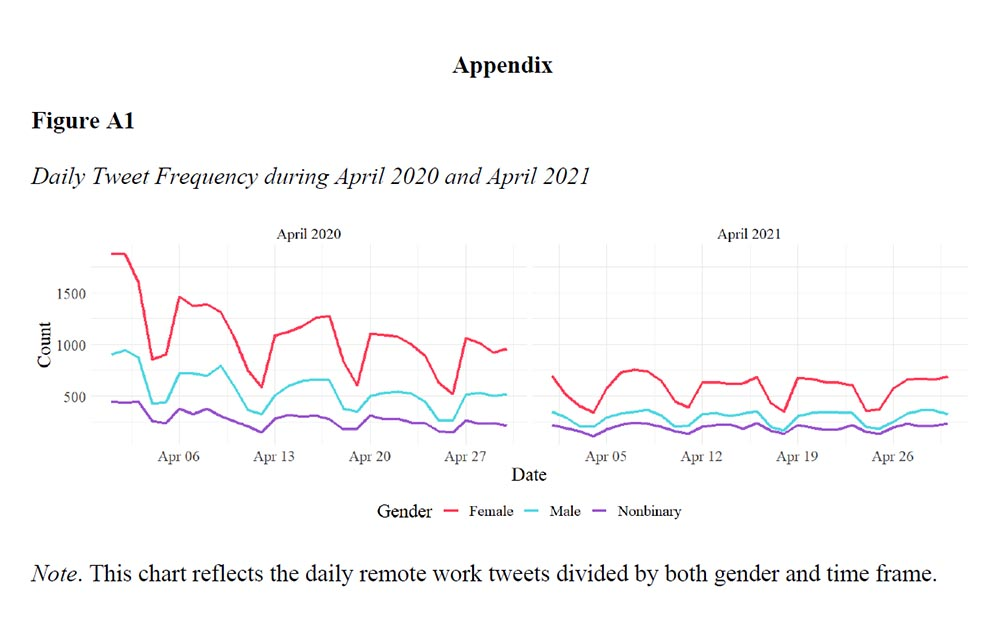
\includegraphics[width=1\linewidth,height=\textheight,keepaspectratio]{images/fig086.jpg}

\subsection*{Information for Inclusion}\label{information-for-inclusion}
\addcontentsline{toc}{subsection}{Information for Inclusion}

\subsubsection*{Research Problem}\label{research-problem}
\addcontentsline{toc}{subsubsection}{Research Problem}

The research problem is the foundation upon which your entire study is built. It is the issue, gap, or challenge that your research aims to address, and it guides the direction of your investigation. Clearly defining the research problem is crucial because it sets the focus for the study and informs the development of research questions, hypotheses, and methods. A well-defined research problem should be specific, measurable, and researchable, meaning that it should be narrow enough to allow for a thorough investigation but broad enough to be significant within the field. For undergraduate students, identifying a research problem involves reviewing existing literature, understanding the current state of knowledge in the field, and pinpointing areas where further exploration is needed. This step requires critical thinking and a deep understanding of the subject matter, as the problem must be both meaningful and feasible to study. The clarity and precision with which you articulate the research problem will determine the relevance and focus of your entire research report.

\subsubsection*{Relevant Theory + Literature}\label{relevant-theory-literature}
\addcontentsline{toc}{subsubsection}{Relevant Theory + Literature}

The relevant theory and literature section is where you contextualize your research within the broader academic landscape. This involves discussing existing theories that relate to your research problem and reviewing previous studies that have addressed similar or related issues. The purpose of this section is to demonstrate your understanding of the current state of knowledge in your field and to identify gaps that your research aims to fill. Theoretical frameworks provide the lens through which you will analyze your data, helping to explain and predict phenomena. A thorough literature review also allows you to build on existing knowledge, showing how your research contributes to ongoing academic discussions. For undergraduate students, this section is an opportunity to engage with the work of others critically, synthesizing different perspectives to justify the need for your study. This step requires extensive reading, analysis, and the ability to connect your research problem with broader theoretical and empirical discussions.

\subsubsection*{Research Questions/Hypotheses}\label{research-questionshypotheses}
\addcontentsline{toc}{subsubsection}{Research Questions/Hypotheses}

Research questions and hypotheses are the specific inquiries or predictions that your study seeks to answer or test. These elements stem directly from your research problem and are critical to guiding your research design and methodology. Research questions are typically open-ended, focusing on exploring or understanding a phenomenon, while hypotheses are statements that predict a relationship between variables and are usually tested through empirical research. Clearly formulated research questions and hypotheses provide a clear direction for your study, helping you stay focused on your objectives throughout the research process. For undergraduate students, developing research questions and hypotheses requires a deep understanding of the research problem and the relevant literature. These elements must be precise, feasible, and aligned with the overall goals of the study. They also form the basis for your research design, influencing everything from the selection of variables to the choice of analytical methods.

\subsubsection*{Conceptual Definition of Variables}\label{conceptual-definition-of-variables}
\addcontentsline{toc}{subsubsection}{Conceptual Definition of Variables}

The conceptual definition of variables involves explaining what each variable represents in the context of your study. This definition is more abstract and theoretical, outlining the meaning and scope of each variable as it relates to your research problem and objectives. Conceptual definitions are important because they establish a common understanding of the variables among your readers and clarify how these variables are connected to the research questions or hypotheses. For undergraduate students, conceptualizing variables requires an understanding of the theoretical framework and how the variables function within that framework. For example, if your study examines ``social media influence,'' you need to define what you mean by ``influence'' conceptually---whether it refers to changes in behavior, attitudes, or perceptions. A clear conceptual definition helps ensure that the variables are measured and analyzed consistently throughout the study.

\subsubsection*{Research Method}\label{research-method}
\addcontentsline{toc}{subsubsection}{Research Method}

The research method section outlines the overall approach you will take to investigate your research problem. This could involve qualitative methods, quantitative methods, or a mixed-methods approach, depending on the nature of your research questions and the type of data you need to collect. The research method you choose will determine how you collect, analyze, and interpret data. For undergraduate students, selecting an appropriate research method involves considering the strengths and limitations of different approaches and how they align with your research objectives. A well-chosen method enhances the validity and reliability of your study, ensuring that your findings are credible and meaningful. This section should also explain why the chosen method is suitable for addressing your research problem, linking it back to the research questions and hypotheses.

\subsubsection*{Operational Definition of Variables}\label{operational-definition-of-variables}
\addcontentsline{toc}{subsubsection}{Operational Definition of Variables}

The operational definition of variables specifies how each variable will be measured or manipulated in your study. Unlike the conceptual definition, which is more abstract, the operational definition is concrete and practical, detailing the exact procedures or instruments you will use to collect data on each variable. For instance, if your conceptual variable is ``academic performance,'' your operational definition might specify that it will be measured by students' grade point averages (GPAs). Operational definitions are crucial because they ensure that variables are measured consistently and accurately, allowing for precise data collection and analysis. For undergraduate students, defining variables operationally requires careful consideration of the tools and methods available for measurement, as well as ensuring that these measurements align with the study's conceptual framework. Clear operational definitions are key to the replicability of your research, as they provide a blueprint for how the study was conducted.

\subsubsection*{Chosen Population}\label{chosen-population}
\addcontentsline{toc}{subsubsection}{Chosen Population}

The chosen population refers to the entire group of individuals or entities that your study seeks to understand or draw conclusions about. This population is defined based on the research problem and objectives, and it should be representative of the broader group that you wish to generalize your findings to. Identifying your chosen population involves specifying characteristics such as age, gender, geographic location, or other relevant factors. For undergraduate students, selecting the appropriate population is a critical step in ensuring the external validity of the study. The chosen population determines the scope of the research and influences decisions about sampling methods and data collection. Clearly defining the population helps to establish the relevance and applicability of your findings to the broader context of your research.

\subsubsection*{Sample Method}\label{sample-method}
\addcontentsline{toc}{subsubsection}{Sample Method}

The sample method details how a subset of the chosen population will be selected for the study. Since it is often impractical to study an entire population, sampling allows researchers to make inferences about the larger group based on the analysis of a smaller, representative sample. There are various sampling methods, including random sampling, stratified sampling, and convenience sampling, each with its advantages and limitations. The sample method must align with the research design and objectives to ensure that the sample accurately represents the population. For undergraduate students, understanding the principles of sampling is essential for making informed decisions about how to select participants and how those selections might influence the study's outcomes. The sample method also affects the study's internal and external validity, as it determines the extent to which the findings can be generalized to the broader population.

\subsubsection*{Data Collection Method}\label{data-collection-method}
\addcontentsline{toc}{subsubsection}{Data Collection Method}

The data collection method describes how data will be gathered from the sample. This could involve surveys, interviews, observations, experiments, or the use of existing data sources. The choice of data collection method depends on the research questions, the nature of the variables, and the overall research design. Each method has its strengths and weaknesses, and it is important to choose one that will provide the most accurate and reliable data for your study. For undergraduate students, selecting a data collection method involves considering factors such as accessibility to the sample, the resources available, and the ethical implications of data collection. The data collection method is critical to the success of the research, as it directly impacts the quality and integrity of the data that will be analyzed and interpreted.

\subsubsection*{Data Cleaning Process}\label{data-cleaning-process}
\addcontentsline{toc}{subsubsection}{Data Cleaning Process}

The data cleaning process is an essential step that occurs after data collection and before data analysis. It involves reviewing the collected data for errors, inconsistencies, or missing values that could skew the results. Data cleaning may involve correcting data entry errors, handling missing data, and ensuring that the dataset is accurate and complete. For undergraduate students, understanding the importance of data cleaning is crucial because it directly affects the validity and reliability of the research findings. A well-executed data cleaning process ensures that the data is ready for analysis, minimizing the risk of bias and inaccuracies. This step also involves making decisions about how to handle anomalies in the data, such as outliers or invalid responses, which could otherwise compromise the study's conclusions.

\subsubsection*{Data Analysis Method}\label{data-analysis-method}
\addcontentsline{toc}{subsubsection}{Data Analysis Method}

The data analysis method refers to the techniques and procedures you will use to examine the cleaned data and draw conclusions based on your research questions or hypotheses. This could involve statistical analysis, thematic analysis, content analysis, or other methods, depending on whether your research is qualitative, quantitative, or mixed-methods. The choice of data analysis method must align with the type of data collected and the overall research design. For undergraduate students, selecting an appropriate data analysis method involves understanding the different types of analysis and how they relate to the research objectives. The data analysis method is critical because it determines how the data will be interpreted, and it ultimately shapes the findings and conclusions of the study. A thorough understanding of data analysis techniques is necessary to ensure that the analysis is both rigorous and appropriate for the research questions being addressed.

\subsubsection*{Results of Analysis}\label{results-of-analysis}
\addcontentsline{toc}{subsubsection}{Results of Analysis}

The results of the analysis section presents the findings of your study based on the data analysis method used. This section should clearly and objectively summarize the outcomes of the analysis, including any statistical results, patterns, or themes identified in the data. The results should be presented in a logical order, often accompanied by tables, charts, or graphs that help to illustrate the findings. For undergraduate students, the results section is an opportunity to communicate what the data reveals without interpretation or bias. It is important to present the results transparently, ensuring that the findings are understandable and accessible to the reader. This section forms the foundation for the discussion, where the implications of these results will be explored in greater depth.

\subsubsection*{Discussion of Findings}\label{discussion-of-findings}
\addcontentsline{toc}{subsubsection}{Discussion of Findings}

The discussion of findings is where you interpret the results of your analysis, relating them back to the research questions, hypotheses, and the broader theoretical framework. This section should explore the significance of the findings, discussing how they contribute to the field, their implications for future research, and how they compare to existing literature. The discussion should also address any unexpected results and offer explanations for these outcomes. For undergraduate students, the discussion section is a chance to demonstrate critical thinking and to connect the results to the broader academic conversation. This section should be thoughtful and insightful, offering a deeper understanding of what the findings mean and why they are important. The discussion also provides an opportunity to reflect on the limitations of the study and suggest directions for future research, acknowledging that no study is without its constraints.

\subsubsection*{Drawn Conclusions}\label{drawn-conclusions}
\addcontentsline{toc}{subsubsection}{Drawn Conclusions}

The drawn conclusions section is where you summarize the key takeaways from your study, based on the findings and the discussion. This section should reiterate the significance of the research problem, the contribution of the study to the field, and the practical or theoretical implications of the findings. Conclusions should be clear and concise, leaving the reader with a strong understanding of what has been learned and how it advances knowledge in the field. For undergraduate students, drawing conclusions involves synthesizing the information presented in the report, distilling the most important insights, and articulating the study's overall contribution. This section should also highlight any recommendations for practice or future research, providing a clear endpoint for the report that reinforces the study's value. The conclusions serve as the final word on your research, leaving a lasting impression on the reader about the significance and impact of your work.

\subsection*{Examples of Formal Reports}\label{examples-of-formal-reports}
\addcontentsline{toc}{subsection}{Examples of Formal Reports}

\subsubsection*{Academic Examples}\label{academic-examples}
\addcontentsline{toc}{subsubsection}{Academic Examples}

There are many different ways to report research in academia. Some of the most common methods include:

\textbf{Research papers}: Research papers are the most common way to report research in academia. They are typically published in academic journals and are written in a formal style.

\textbf{Conference papers}: Conference papers are presented at academic conferences. They are typically shorter than research papers and are written in a more informal style.

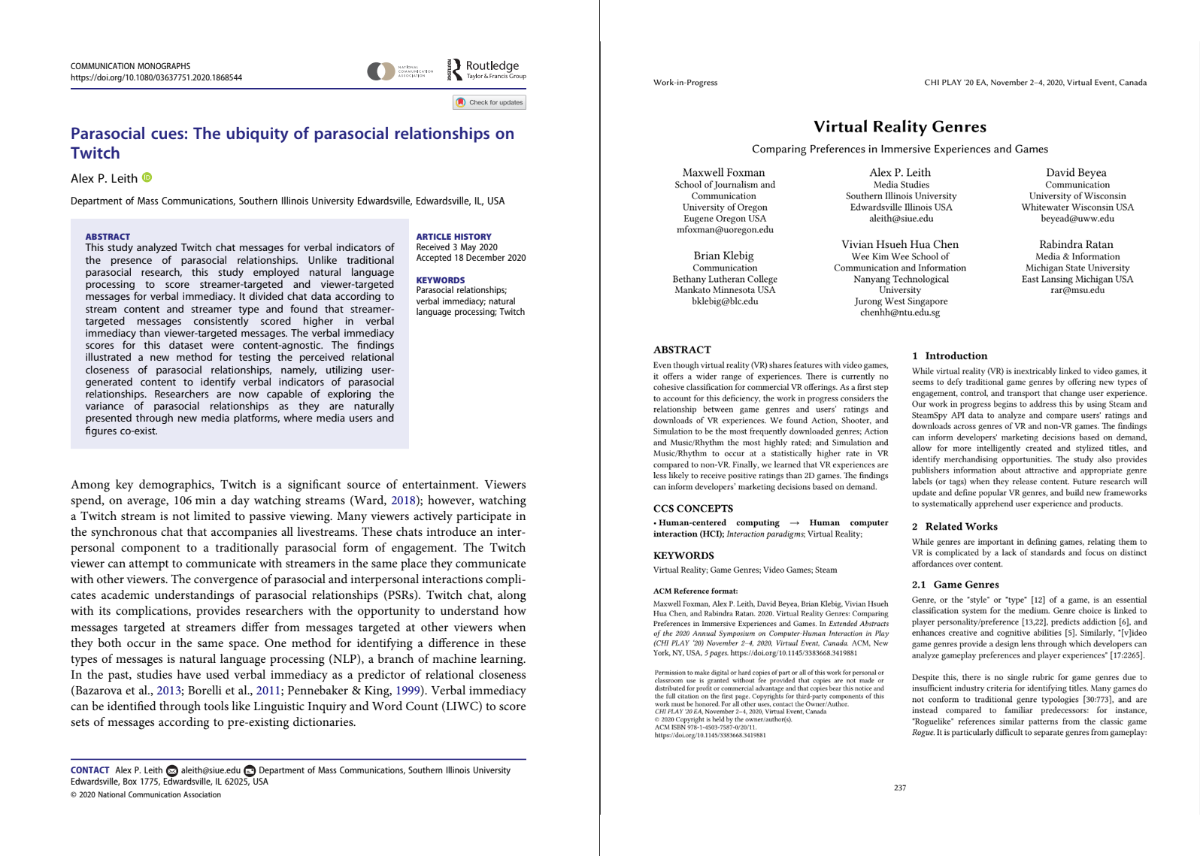
\includegraphics[width=1\linewidth,height=\textheight,keepaspectratio]{images/papers.png}

\textbf{Theses and dissertations}: Theses and dissertations are written by graduate students to complete their degree requirements. They are typically longer and more comprehensive than research papers.

\textbf{Books}: Books are another way to report research. They are typically written by experts in a particular field and can be a good way to communicate research to a wider audience.

\textbf{Reports}: Reports are written for a specific audience, such as a government agency or a business. They are typically shorter than research papers and focus on a specific topic.

\textbf{Presentations}: Presentations are a way to share research with a live audience. They can be given at conferences, workshops, or other events.

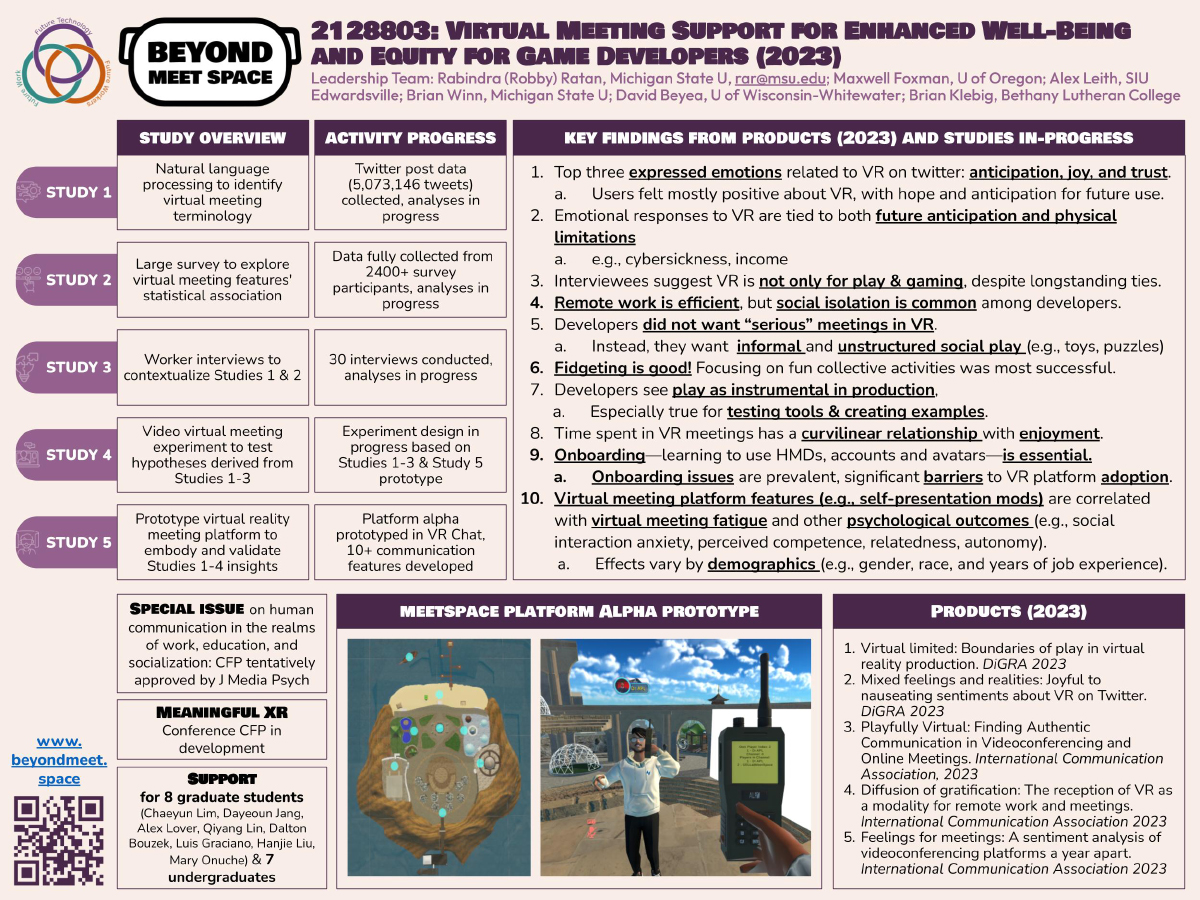
\includegraphics[width=1\linewidth,height=\textheight,keepaspectratio]{images/BMS 2023 poster final.jpg}

\textbf{Blogs and social media}: Blogs and social media can be used to share research with a wider audience. They are a good way to communicate research in a more informal way.

The best way to report research depends on the specific research project and the intended audience. However, all of these methods can be effective ways to communicate research findings and to contribute to the academic community.

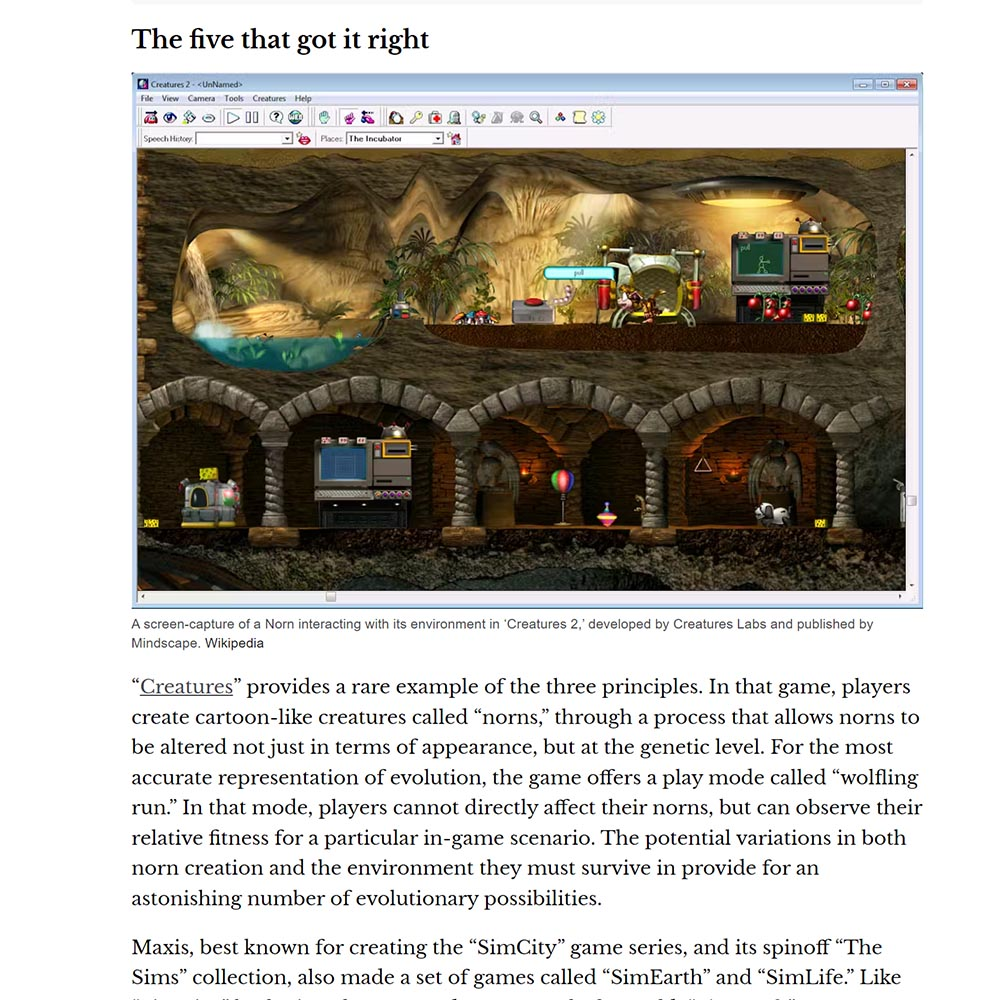
\includegraphics[width=1\linewidth,height=\textheight,keepaspectratio]{images/fig091.jpg}

\subsubsection*{Industry Examples}\label{industry-examples}
\addcontentsline{toc}{subsubsection}{Industry Examples}

There are many different ways to report research in industry. Some of the most common methods include:

\textbf{White papers}: White papers are a type of report that is commonly used in industry to present research findings to a specific audience. They are typically written in a clear and concise style and focus on a specific topic.


\includegraphics[width=1\linewidth,height=\textheight,keepaspectratio]{images/white_paper.png}

\textbf{Executive summaries}: Executive summaries are a brief overview of a white paper or other research report. They are typically written for senior executives and other decision-makers.

\textbf{Presentations}: Presentations are a way to share research findings with a live audience. They can be given at company meetings, conferences, or other events.

\textbf{Blogs and social media}: Blogs and social media can be used to share research findings with a wider audience. They are a good way to communicate research in a more informal way.

\textbf{Press releases}: Press releases are a way to share research findings with the media. They are typically written in a clear and concise style and focus on the key findings of the research.

\textbf{Technical reports}: Technical reports are a detailed document that describes the research methods and findings. They are typically written for a technical audience.

The best way to report research in industry depends on the specific research project and the intended audience. However, all of these methods can be effective ways to communicate research findings and to contribute to the industry community.

\chapter{Writing for a Public Audience}\label{writing-for-a-public-audience}

This chapter equips students with practical skills and techniques for effectively translating complex research findings into different media formats. It emphasizes the importance of adapting academic content into engaging, accessible forms suitable for a public audience, focusing on three specific media types: feature articles, infographics with associated whitepaper, and news broadcast scripts with storyboarding.

\section{Communication Strategies}\label{communication-strategies}

\subsection*{Crafting Compelling Messages}\label{crafting-compelling-messages}
\addcontentsline{toc}{subsection}{Crafting Compelling Messages}

In the field of mass communication, effectively conveying research findings is as important as conducting the research itself. Particularly in domains like social media analytics, where vast amounts of data are involved, the ability to present your research in a compelling and accessible manner can significantly influence its impact. Crafting a compelling message involves a delicate balance between maintaining the analytical rigor of your work and ensuring that your findings are understandable and engaging for a wide audience, including those who may not have a background in data analysis.

The key to achieving this balance lies in transforming complex datasets into narratives that resonate with your audience. This transformation begins with a deep understanding of your data---recognizing patterns, identifying key insights, and understanding the broader implications of your findings. However, the process doesn't end there. To truly engage your audience, you must present these insights in a way that is not only informative but also emotionally and intellectually stimulating. This requires the integration of storytelling techniques, visual enhancements, and strategic calls to action, all of which are essential tools in the dissemination of research in mass communications.

Moreover, the tools you choose to convey your message play a crucial role in how your research is perceived. Analytical tools such as RStudio are invaluable for processing and visualizing data, allowing you to identify and highlight key insights. However, to make these insights accessible and engaging, it is often necessary to go beyond traditional data visualization techniques. Creative platforms like Adobe Express offer a range of features that can help you craft visually appealing and emotionally resonant narratives. By combining the analytical power of tools like RStudio with the creative capabilities of platforms like Adobe Express, you can create messages that not only inform but also inspire action and change.

\subsubsection*{Employing Storytelling Techniques}\label{employing-storytelling-techniques}
\addcontentsline{toc}{subsubsection}{Employing Storytelling Techniques}

Storytelling is a powerful tool in mass communications, and its importance in the dissemination of research cannot be overstated. When you approach your data with a storytelling mindset, you look beyond the numbers and statistics to uncover the narrative that lies within. This narrative could be about a trend, a significant shift, or an unexpected discovery. By framing your findings as a story, you create a structure that is familiar and engaging to your audience. A well-crafted narrative typically has a clear beginning, where you introduce the problem or question your research addresses; a middle, where you present your findings and their implications; and an end, where you offer conclusions and suggest potential actions.

To make your story more relatable, it is important to humanize your data. This means connecting your findings to real-world experiences and situations that your audience can relate to. For example, if your research focuses on social media trends, consider incorporating case studies or hypothetical scenarios that illustrate how these trends impact individuals or communities. This approach helps bridge the gap between abstract data and the lived experiences of your audience, making your findings more tangible and meaningful.

In addition to humanizing your data, creating relatable characters can further enhance the impact of your narrative. These ``characters'' might be typical users, communities, or organizations that are affected by the trends or issues you have studied. By centering your narrative around these characters, you create a story that is not only informative but also emotionally engaging. This technique helps your audience see the relevance of your research in a more personal and immediate way, fostering a deeper connection with the subject matter.

\subsubsection*{Visual Enhancements through Adobe Express}\label{visual-enhancements-through-adobe-express}
\addcontentsline{toc}{subsubsection}{Visual Enhancements through Adobe Express}

Visual elements are another critical component of effective message crafting, particularly in the context of mass communication. Visuals have the power to simplify complex ideas, highlight key points, and make your research more accessible to a broader audience. Adobe Express is an excellent tool for creating such visuals, offering a wide range of options for designing infographics, charts, and thematic imagery that complement and enhance your narrative.

When creating visuals, it is important to ensure that they align with the overall tone and theme of your message. Visual consistency---using a uniform color palette, font style, and design elements---helps build a cohesive and recognizable brand for your research. This consistency not only makes your presentation more professional but also reinforces the key messages of your research, making them more memorable for your audience.

Another important consideration when designing visuals is the need to simplify complexity. One of the main challenges in communicating research findings is making complex ideas understandable without oversimplifying them. Adobe Express offers user-friendly tools that allow you to create visuals that break down complicated concepts into more manageable and digestible components. Whether you are illustrating the results of a data analysis or highlighting the key takeaways from your research, well-designed visuals can make a significant difference in how your message is received and understood.

\subsubsection*{Creating Clear and Engaging Messages}\label{creating-clear-and-engaging-messages}
\addcontentsline{toc}{subsubsection}{Creating Clear and Engaging Messages}

In the context of mass communication, the ability to convey research findings to a public audience effectively is crucial. Public audiences often do not have the same level of familiarity with the subject matter as experts do, so researchers must approach communication with a focus on clarity and engagement. This involves not only simplifying the content but also making it interesting and relevant to the audience. The goal is to transform complex research into messages that are easily understood and appreciated by a broad audience. This section delves into strategies for achieving this balance, ensuring that your communication is both clear and captivating.

\textbf{Simplicity is Key}

The foundation of effective communication lies in simplicity. Even the most groundbreaking research can fail to make an impact if it is not communicated in a way that is accessible to the general public. Academic jargon, technical terms, and overly complex explanations can create barriers between your research and the audience. Therefore, simplifying your message without compromising its accuracy is essential.

To achieve simplicity, start by avoiding jargon. Technical terms may be second nature to you as a researcher, but for the uninitiated, they can be confusing and alienating. Instead of using specialized language, opt for plain language that is straightforward and easy to understand. This does not mean oversimplifying or dumbing down your content; rather, it involves translating complex ideas into terms that a non-expert audience can grasp.

Another effective strategy for simplifying your message is the use of analogies and metaphors. These rhetorical devices can help make abstract or complicated concepts more relatable by connecting them to familiar experiences or ideas. For instance, explaining a complex algorithm by comparing it to a recipe or a decision-making process can make the concept more tangible for your audience. Analogies and metaphors not only aid in understanding but also make your message more memorable.

Breaking down complex ideas into smaller, more digestible parts is another critical aspect of simplicity. When presenting research findings, consider deconstructing them into step-by-step explanations that build on each other. This incremental approach allows your audience to follow along more easily, ensuring that they are not overwhelmed by the complexity of the information. By guiding your audience through your findings in a logical and straightforward manner, you help them build a clear and coherent understanding of your research.

\textbf{Be Concise}

In today's fast-paced world, where attention spans are often short, conciseness is a vital component of effective communication. Being concise does not mean leaving out important information; rather, it involves focusing on what is most important and delivering it in a way that captures and holds your audience's attention.

To be concise, begin by identifying the key points of your research. What are the most significant findings? What do you want your audience to remember? By honing in on these essential aspects, you can eliminate extraneous details that might distract or confuse your audience. This focus on the core message helps ensure that your communication is both impactful and memorable.

Highlighting the significance of your findings is another way to maintain conciseness while enhancing engagement. It is not enough to present your research; you must also explain why it matters. Connect your findings to real-world issues, societal benefits, or practical applications to demonstrate their relevance. By clearly articulating the importance of your research, you give your audience a reason to care, which helps sustain their interest.

Visual aids, such as charts, graphs, and infographics, are invaluable tools for summarizing key points succinctly. Visuals can convey complex information quickly and effectively, making them an ideal complement to concise communication. A well-designed infographic, for example, can encapsulate an entire research project's key findings in a single, visually engaging format. This not only aids in comprehension but also makes your message more visually appealing, which can further enhance its impact.

Creating clear and engaging messages involves a careful balance of simplicity and conciseness. The aim is not to oversimplify the content but to make it accessible and interesting to a broader audience. By focusing on these principles, researchers can bridge the gap between academic research and public understanding, ensuring that their work is not only recognized but also valued by society. This approach fosters a greater appreciation for the role of research in addressing societal challenges and advancing knowledge, ultimately contributing to a more informed and engaged public.

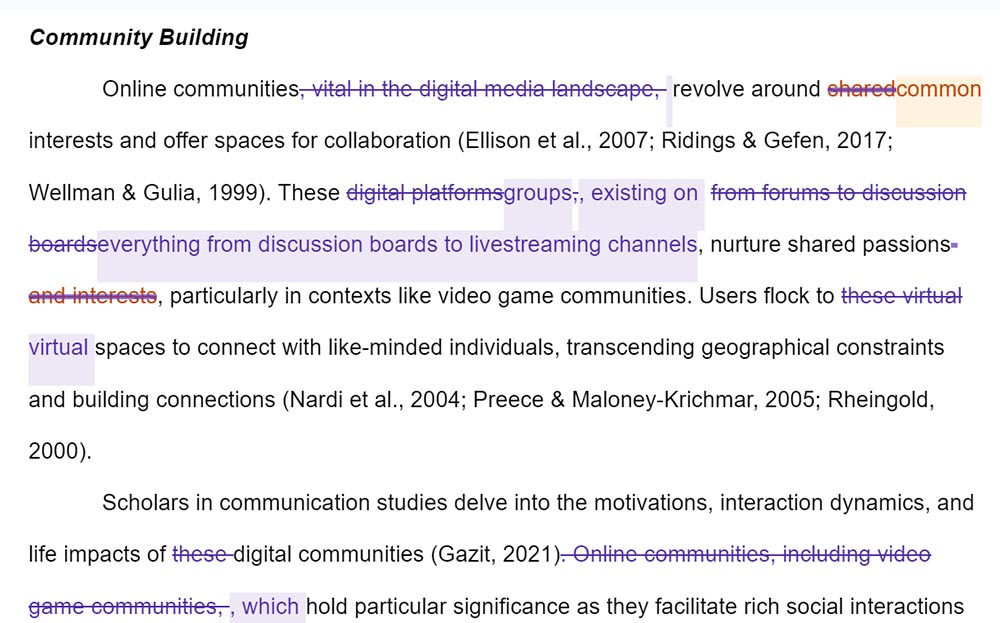
\includegraphics[width=1\linewidth,height=\textheight,keepaspectratio]{images/fig087.jpg}

\subsubsection*{Employing Storytelling Techniques}\label{employing-storytelling-techniques-1}
\addcontentsline{toc}{subsubsection}{Employing Storytelling Techniques}

In the dissemination of research findings, particularly within the realms of social media analytics and mass communication, storytelling emerges as an essential tool that goes beyond simply presenting data. It transforms statistics and analyses into narratives that engage, inform, and inspire the audience. Storytelling in research communication serves to bridge the gap between complex information and the audience's understanding, making data not only accessible but also meaningful. By embedding research findings within a well-crafted story, you can capture your audience's attention, evoke emotional responses, and facilitate a deeper understanding of the material. The following explores various storytelling techniques that can significantly enhance the impact of your research communication.

\textbf{Narrative Structures}

The foundation of any compelling story lies in its structure. A well-organized narrative provides a roadmap that guides the audience through the complexities of your research, making it easier for them to follow and engage with your findings. Structuring your message as a story involves several key elements.

To set the stage, begin your narrative with a strong introduction that outlines the context and importance of your research. This introduction should not merely present background information but should also establish the relevance of the research question or problem you are addressing. By doing so, you create a sense of anticipation and curiosity in your audience, drawing them into the story you are about to tell. This stage is crucial because it sets the tone for the rest of your narrative and provides the audience with a reason to care about your findings.

As the narrative progresses, develop the plot by delving into the core of your research---this is where the action happens. The middle section of your story should cover the analysis and findings of your research in a way that is both clear and engaging. Here, the journey from hypothesis to conclusion should be laid out in a logical and compelling manner. It's important to maintain a balance between detail and clarity, ensuring that your audience can follow the research process and appreciate the significance of the discoveries made. This section is the heart of your narrative, where the intricacies of your research are unpacked and explored.

Finally, conclude your narrative by tying the findings back to the original problem or question. This conclusion should not only summarize your research but also emphasize its implications and potential applications. A strong ending leaves your audience with a clear understanding of how your research contributes to the field and why it matters. By concluding with impact, you ensure that your audience walks away with a lasting impression of the importance and relevance of your work.

\textbf{Analogies and Examples}

Analogies and examples are powerful storytelling tools that can help bridge the gap between complex research concepts and the audience's prior knowledge. They serve to make abstract ideas more concrete and relatable by connecting them to familiar experiences.

Analogies work by drawing parallels between a complex concept and a situation that is more commonly understood. For example, if you are explaining a network analysis in social media research, you might compare it to understanding social dynamics within a small community. Just as one might observe how individuals within a community interact, form groups, or influence one another, network analysis examines how users in social media networks connect, share information, and influence each other. This comparison makes the concept more accessible to those who may not be familiar with the technical aspects of network analysis, providing them with a mental framework to better understand your research.

Real-world examples, on the other hand, ground your research findings in tangible, everyday scenarios. By illustrating how your findings apply in real-life situations, you demonstrate the practical significance of your research. For instance, if your research identifies a trend in social media usage among teenagers, providing an example of how this trend influences their behavior or decision-making in real life makes the data more relevant and impactful. Examples not only help clarify complex ideas but also serve as proof points that reinforce the validity and importance of your findings.

\textbf{Personalize Your Message}

Personalizing your message by adding a human element can significantly enhance its appeal and relatability. When research is connected to real people and their experiences, it becomes more than just data---it becomes a narrative that resonates on a personal level.

One way to personalize your message is by highlighting the human impact of your research. Whenever possible, incorporate stories or case studies that illustrate how individuals or communities are affected by the issues your research explores. For example, if your research focuses on the effects of social media on mental health, you might include a case study of a teenager whose mental health was impacted by their social media usage. This approach not only makes your research more relatable but also evokes empathy, drawing your audience into the narrative on an emotional level.

Engaging the audience emotionally is a powerful way to enhance the impact of your research. While it's important to remain objective and accurate, recognizing the emotional dimensions of your research can help foster a deeper connection with your audience. By presenting your findings in a way that touches on the emotions of your audience---whether it's concern, hope, curiosity, or inspiration---you make the research more memorable and impactful. This emotional engagement is not about manipulating feelings but about ensuring that the human relevance of your research is front and center.

Employing storytelling techniques in research communication is not about embellishing or distorting facts but about presenting them in a way that is engaging, understandable, and memorable. Through well-organized narrative structures, the use of analogies and examples, and personalizing your message, you can transform your research from a collection of data points into a compelling story that informs, inspires, and instigates change. By doing so, you not only enhance the communication of your research findings but also contribute to a broader understanding and appreciation of the value of academic research in society.

\subsubsection*{Incorporating Visual Elements}\label{incorporating-visual-elements}
\addcontentsline{toc}{subsubsection}{Incorporating Visual Elements}

In today's digital landscape, where information is rapidly consumed and often fleetingly retained, the role of visual elements in research communication cannot be overstated. Visuals have the unique ability to condense complex information into more digestible forms, making them indispensable tools for researchers, especially when aiming to engage public audiences. This is particularly true in fields such as social media analytics, where data can be dense and difficult to interpret without visual aids. Effective visuals not only clarify complex data but also enhance the overall appeal and shareability of research findings. This section explores strategies for incorporating visual elements into your research communication, ensuring that your message is both impactful and accessible.

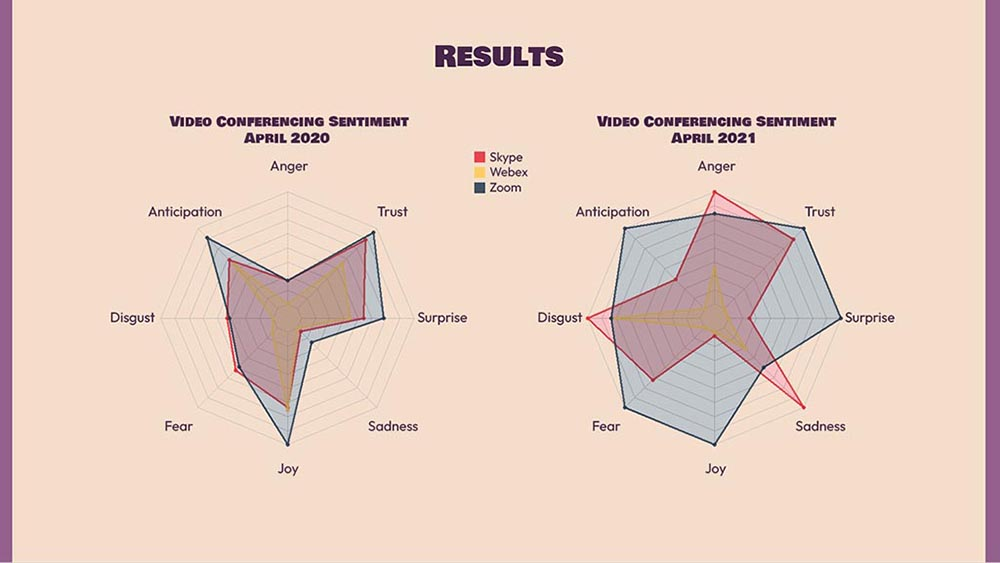
\includegraphics[width=1\linewidth,height=\textheight,keepaspectratio]{images/fig089.jpg}

\textbf{Data Visualizations}

Data visualizations are perhaps the most critical visual tools in research dissemination. They translate raw data into visual formats that can tell a compelling story, making patterns, trends, and relationships within the data more apparent to your audience. To create effective data visualizations, one must consider both the technical and aesthetic aspects of design.

Leveraging the capabilities of RStudio is a strategic approach to creating high-quality data visualizations. RStudio, with its extensive libraries such as \texttt{ggplot2}, allows researchers to produce customized, publication-quality visuals that can effectively communicate the nuances of their findings. Whether you're illustrating trends over time, comparing different groups, or mapping spatial data, these tools offer the flexibility to tailor your visualizations to highlight the most critical aspects of your research.

Clarity should be the guiding principle when designing data visualizations. While it might be tempting to include as much information as possible, simplicity often leads to more effective communication. Your audience should be able to understand the key message of your visualization at a glance. This requires careful consideration of the visual elements---such as color, scale, and labeling---ensuring that they enhance rather than obscure the data's meaning. Emphasizing key data points and trends can help direct the audience's attention to the most important findings.

Annotations are another powerful tool within data visualizations. By including explanatory notes directly on your visualizations, you guide the audience through the data, making it easier for them to grasp complex concepts. Annotations can highlight significant points, explain the implications of certain trends, or provide context that might not be immediately apparent from the data alone. This additional layer of information can be particularly helpful in making your research more accessible to those who may not be familiar with the technical aspects of the data.

\textbf{Enhancing Visuals with Adobe Express}

While data visualizations are crucial, not all visuals in research communication are data-driven. For other types of visual content, Adobe Express offers a versatile platform that can significantly enhance the visual appeal and effectiveness of your research communication. Adobe Express is particularly useful for creating infographics, promotional graphics, and supplementary multimedia content that can make your research more engaging and shareable.

Infographics are an excellent way to summarize your research findings in a format that is both visually appealing and easy to understand. Adobe Express allows you to design custom infographics that can effectively distill complex information into its most essential points. These visuals can be particularly useful for communicating with non-expert audiences or for promoting your research on social media platforms, where attention spans are often limited.

Beyond static visuals, Adobe Express can also help you create supplementary multimedia content, such as short videos or animated graphics. These dynamic elements can further elucidate your findings, making them more engaging and easier to understand. For example, a short video summarizing the key points of your research, combined with animated visualizations, can capture the audience's attention in ways that static text or images alone might not. This type of content is especially valuable in the digital age, where multimedia communication is increasingly the norm.

Adobe Express also offers a wide array of templates and design elements that can be customized to suit the theme and tone of your research. This accessibility is particularly beneficial for those who may not have a background in graphic design, allowing you to create professional-quality visuals without the need for extensive design skills. By using these tools, you can ensure that your visual elements are not only effective but also polished and professional.

\textbf{Consistency in Design}

Maintaining a consistent visual style across all your research communication materials is essential for building a coherent and recognizable brand for your work. Consistency in design helps reinforce your research identity and ensures that your message is communicated clearly and effectively across different platforms and audiences.

Start by choosing a color scheme and typography that reflects the tone and subject matter of your research. These elements should be consistent across all your visuals, whether they are data visualizations, infographics, or promotional graphics. A consistent color scheme and typography not only make your materials more visually cohesive but also contribute to the overall professionalism of your communication.

Thematic consistency is equally important. All visual elements used in your research communication should share a common theme or motif that ties them together. This could be a recurring visual element, such as a specific shape or iconography, or a consistent layout style that is applied across different materials. Thematic consistency strengthens the narrative flow of your communication and makes it easier for your audience to recognize and connect with your research.

Incorporating visual elements into research communication is not merely about enhancing aesthetics; it is about deepening engagement and facilitating understanding. Through strategic use of data visualizations and creative visuals, researchers can effectively bridge the gap between complex data and public audiences. By doing so, you ensure that your findings are not only seen but also understood and appreciated by a broader spectrum of viewers, ultimately increasing the impact and reach of your work.

\section{Common Formats}\label{common-formats}

\subsection{Feature Article}\label{feature-article}

\subsubsection*{Writing Style and Tone}\label{writing-style-and-tone}
\addcontentsline{toc}{subsubsection}{Writing Style and Tone}

When transforming a dense academic research report into a feature article, the primary goal is to craft a narrative that is both engaging and informative. This process requires a significant shift in writing style and tone from the formal, structured approach typical of academic writing to one that is accessible and appealing to a broader audience. The art of writing a feature article lies in balancing the need to convey complex ideas accurately while making them understandable and interesting to non-experts.

\subsubsection*{Clarity and Engagement}\label{clarity-and-engagement}
\addcontentsline{toc}{subsubsection}{Clarity and Engagement}

One of the most critical aspects of writing for a public audience is the ability to simplify complex concepts without losing their essence. Academic research often involves specialized jargon and technical terms that can be challenging for a lay audience to grasp. To bridge this gap, it is essential to break down these terms into everyday language that resonates with the reader. Analogies and comparisons can be particularly effective in this regard. For instance, a complex statistical method might be explained through a relatable analogy, such as comparing it to sorting through a large stack of mail to find specific letters. This approach helps demystify the research, making it more accessible to those who may not have a background in the subject.

Maintaining reader interest throughout the article is another crucial element. Unlike academic papers, which are often read by peers within a specific field, a feature article must capture the attention of a broader audience, many of whom might not be immediately interested in the topic. A storytelling approach can be highly effective here. By guiding the reader through the research as if they were discovering the findings themselves, the writer can create a sense of intrigue and involvement. Starting with a compelling hook---perhaps a surprising statistic or a thought-provoking question---can draw readers in, while a logically flowing narrative keeps them engaged. The article should build towards a clear conclusion, with each section seamlessly leading to the next, ensuring that the reader remains invested in the story being told.

Striking the right tone is also key to crafting an engaging feature article. While the writing should be accessible and conversational, it must also maintain a level of professionalism appropriate for the subject matter. This balance ensures that the article is both credible and approachable. The tone should not be overly casual, as this can undermine the seriousness of the research, but it should avoid the stiffness of academic prose. The aim is to make the content feel like a dialogue rather than a lecture, encouraging readers to engage with the material rather than passively receive it.

\href{https://medium.com/@nishiyama.ry/data-analysis-problematic-and-exploitative-beauty-contests-in-japanese-universities-fe551d31fa66}{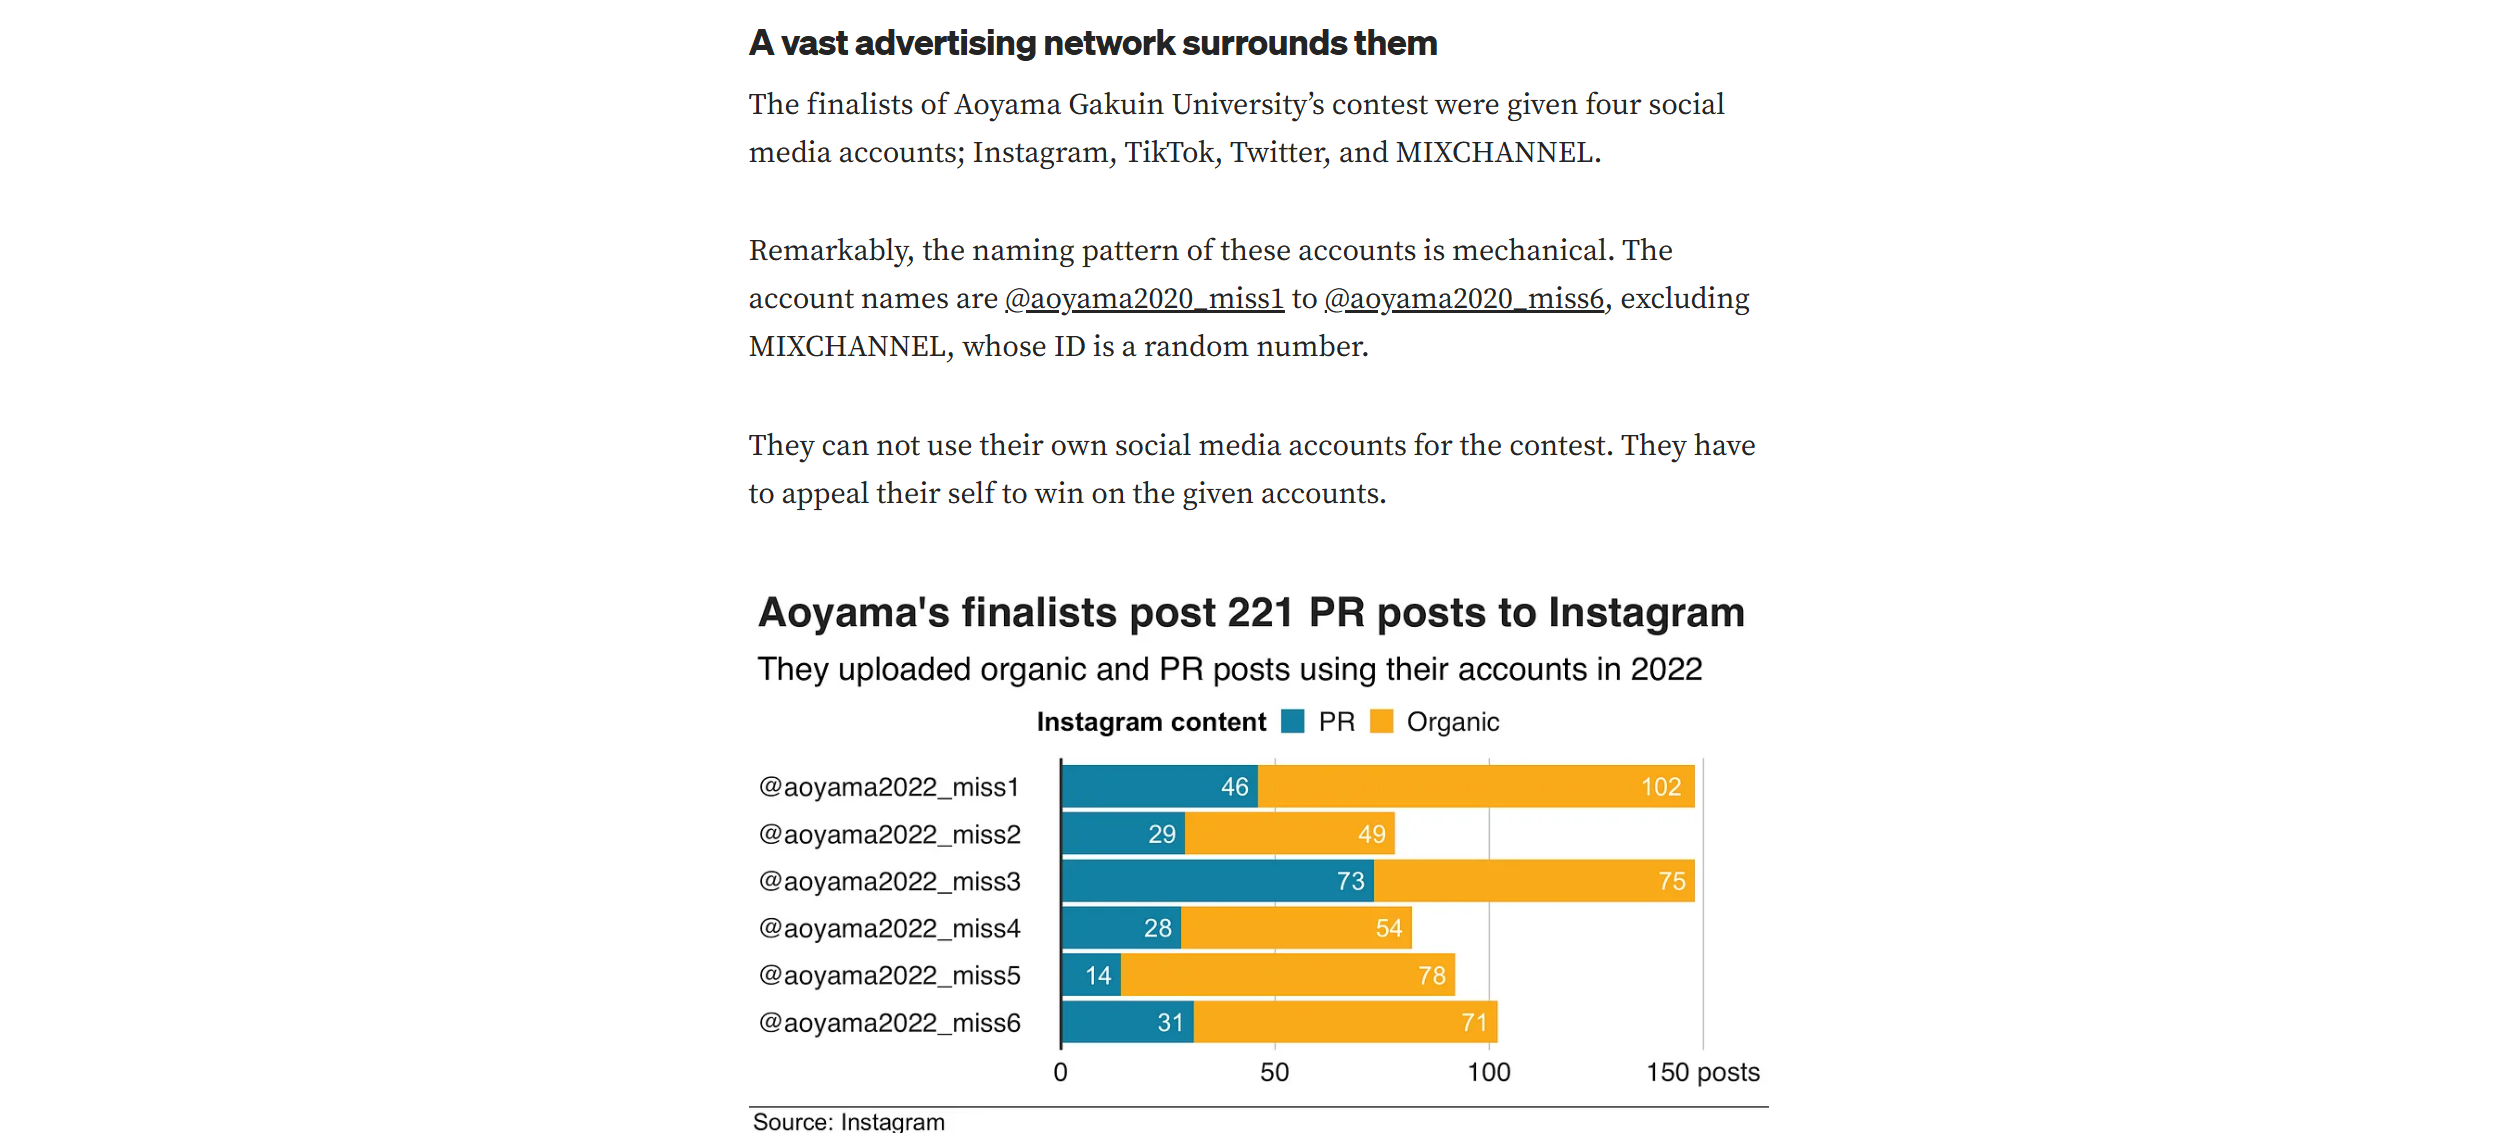
\includegraphics[width=1\linewidth,height=\textheight,keepaspectratio]{images/feature-article.png}}

\subsubsection*{Structuring the Article}\label{structuring-the-article}
\addcontentsline{toc}{subsubsection}{Structuring the Article}

The structure of a feature article plays a significant role in how effectively it communicates the research. A well-crafted headline is the first step in this process. The headline should be catchy and encapsulate the essence of the research, offering a snapshot of what the article will cover. It needs to be intriguing enough to entice readers to click on or pick up the article, but also clear enough to give them an accurate idea of the content.

Subheadings are another important structural element, as they guide the reader through the different sections of the article. In a research-focused feature, subheadings can be used to break down the article into manageable sections, such as the introduction of the research question, the methodology, the key findings, and the implications. This organization not only helps readers navigate the article but also allows them to quickly locate the information that is most relevant to their interests. A logical structure is essential; each section should flow naturally from the previous one, building a cohesive narrative that is easy to follow.

The narrative flow of the article is central to its effectiveness. The article should begin with a strong lead that sets the stage for the research, providing enough context to make the topic relatable and interesting to the reader. The introduction should establish the problem or question the research addresses, giving readers a reason to care about the findings. Following this, the article should provide a summary of the methodology used, explaining the research process in terms that are understandable to a general audience. This section should be concise, focusing on the aspects of the methodology that are most relevant to the findings. The key findings themselves should be presented clearly, with a focus on their implications and potential impact. The conclusion should tie everything together, reflecting on the significance of the research and exploring any potential future developments in the field.

Incorporating quotes and examples throughout the article can add depth and interest, making the content more relatable and authoritative. Quotes from the research itself or from experts in the field can lend credibility to the article, providing firsthand insights into the study's significance. Real-world examples can help illustrate abstract concepts, making them more tangible for the reader. For instance, if the research involves the impact of social media on mental health, including a case study or anecdote about an individual's experience can make the findings more relatable and compelling.

\subsection{Infographic with White Paper}\label{infographic-with-white-paper}

Presenting research findings through an infographic accompanied by a white paper is an effective method for communicating complex data in a visually engaging and accessible format, while also providing the necessary depth and context for a comprehensive understanding of the research. The infographic simplifies the key points of the research, making it appealing and easy to grasp for a broader audience. In contrast, the white paper delves into the details, offering a thorough explanation and interpretation of the data presented in the infographic. This dual approach allows for both immediate impact and in-depth analysis, catering to different audience needs.

\subsubsection*{Dividing Content}\label{dividing-content}
\addcontentsline{toc}{subsubsection}{Dividing Content}

When developing an infographic with an accompanying white paper, selecting the most relevant information to feature in each component is crucial for effective communication. The first step is identifying the core elements of the research that will be the focus of the infographic. These should be the findings or data points that are most impactful, visually striking, and central to the research's overall message. The infographic's purpose is to distill the research down to these essential points, presenting them in a way that is immediately understandable and engaging. This might include key statistics, major findings, or significant trends that can be easily visualized through graphs, charts, or other visual representations.

The selection of information for the infographic should be guided by its potential to capture the audience's attention and convey the essence of the research in a concise format. Complex details, nuanced explanations, and background information, while important, are better suited for the white paper. The infographic should avoid overcrowding with too much data or text, as this can overwhelm the viewer and diminish the visual impact. Instead, the focus should be on a few powerful visuals that communicate the key messages clearly and effectively. For instance, a single well-designed chart that highlights a critical finding can be more effective than multiple charts that attempt to convey too much information at once.

In contrast, the white paper should provide the depth and context that the infographic cannot. After identifying the key points for the infographic, the next step is to determine what additional information is necessary to fully explain and support these points in the white paper. The white paper should include detailed explanations of the methodology, in-depth analysis of the findings, and a discussion of the broader implications of the research. It should also address any limitations of the study, explore alternative interpretations of the data, and provide background information that helps to contextualize the findings. This ensures that the audience not only understands the data but also appreciates its significance within the larger research framework.

The white paper should be seen as an extension of the infographic, filling in the gaps and providing the reader with a comprehensive understanding of the research. While the infographic grabs attention and delivers the highlights, the white paper answers the questions that the infographic might raise. For example, if the infographic presents a striking statistic about a correlation between two variables, the white paper should explain how that correlation was discovered, why it is significant, and what it means in practical terms. This detailed explanation helps to reinforce the credibility of the research and provides the audience with the tools they need to interpret the data correctly.

\href{https://winefolly.com/deep-dive/simple-food-and-wine-pairing/}{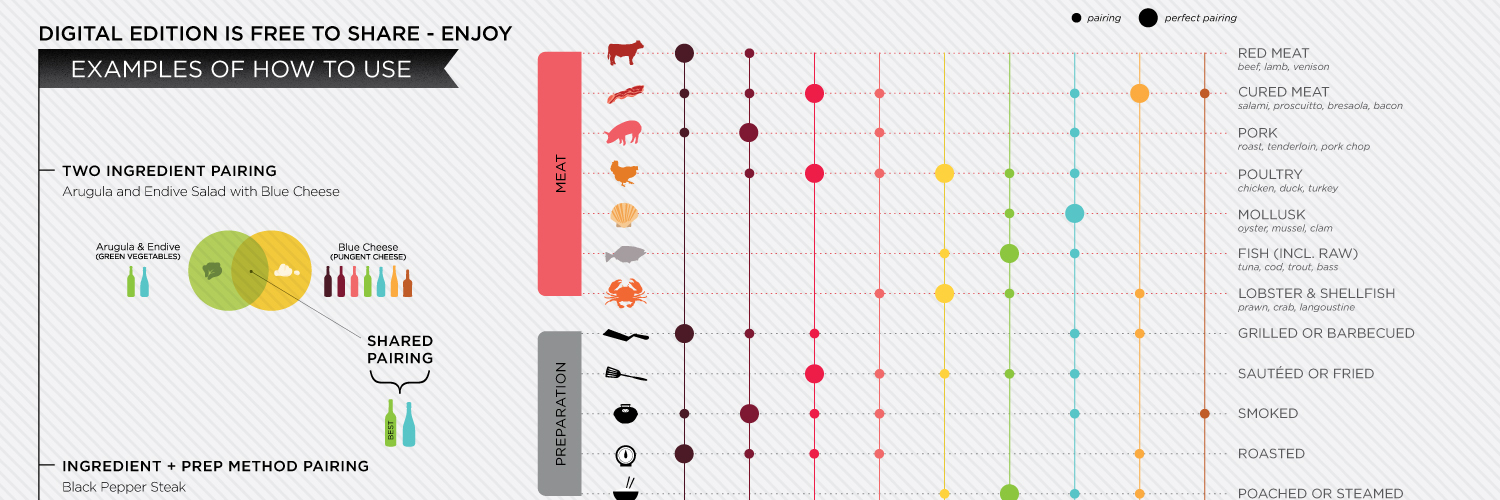
\includegraphics[width=1\linewidth,height=\textheight,keepaspectratio]{images/infographic.jpg}}

\subsubsection*{Structuring the White Paper}\label{structuring-the-white-paper}
\addcontentsline{toc}{subsubsection}{Structuring the White Paper}

Structuring the white paper effectively is key to ensuring that it complements the infographic while providing the necessary depth and detail. The white paper should begin with an introduction that not only explains the purpose of the infographic but also outlines the research problem or question, the methodology, and the key findings. This introduction sets the stage for the reader, helping them understand what the infographic is about and why the information it presents is important.

The body of the white paper should be organized in sections that correspond to the different parts of the infographic. For each section of the infographic, the white paper should provide a more detailed explanation, discussing the data in depth and offering insights that are not immediately apparent from the visual alone. For instance, if the infographic features a graph showing a trend over time, the corresponding section in the white paper might explain how the data was collected, what the trend suggests about the broader research question, and how it compares to previous studies in the field.

In addition to supporting the infographic, the white paper should include sections that discuss aspects of the research that are too complex or detailed to be included in the visual. This might include a thorough discussion of the research methodology, including any challenges faced during data collection or analysis, as well as a discussion of the study's limitations and potential areas for further research. The white paper should also provide a broader context for the research, explaining how it fits into the existing body of knowledge and what implications it might have for future studies or practical applications.

The conclusion of the white paper should tie together the key points presented in both the infographic and the text, reinforcing the main message of the research. This section should also offer a call to action, inviting the audience to engage further with the research, whether by applying its findings, exploring related topics, or considering the implications for their own work or interests.

\subsection*{News Broadcast Script with Storyboarding}\label{news-broadcast-script-with-storyboarding}
\addcontentsline{toc}{subsection}{News Broadcast Script with Storyboarding}

Adapting a research paper into a news broadcast script and accompanying storyboard involves transforming detailed academic content into a format that is both visually engaging and easily digestible for a general audience. This process requires a careful balance between maintaining the integrity of the research and ensuring that the narrative is compelling and accessible. The news broadcast format demands clarity, brevity, and an emphasis on the visual storytelling elements that capture and retain viewer interest. By focusing on these elements, the researcher can effectively communicate complex ideas in a way that resonates with a broad audience.

\subsubsection*{Writing the Script}\label{writing-the-script}
\addcontentsline{toc}{subsubsection}{Writing the Script}

The first step in adapting a research paper into a news broadcast is crafting the script. The script serves as the foundation of the broadcast, guiding both the spoken word and the accompanying visuals. In broadcast journalism, the importance of a strong lead cannot be overstated. The lead is the opening statement or segment that captures the essence of the research and draws the viewer in immediately. Given that audience attention spans are often limited, especially in a broadcast format, the lead must be concise and impactful, conveying the most critical aspect of the research within the first few seconds. This could be a striking statistic, a surprising finding, or a provocative question related to the research topic.

Once the lead has captured the audience's attention, the script must continue to communicate the research in clear and concise language. Unlike academic writing, where complex sentences and jargon are often used to convey detailed information, broadcast scripts must be straightforward and easily understood by a lay audience. The goal is to distill the research into its most essential points, avoiding unnecessary complexity and ensuring that the message is both clear and engaging. This often involves simplifying technical language and breaking down complex concepts into more digestible parts, all while maintaining the accuracy and integrity of the original research.

In addition to clear language, the use of sound bites is a critical element of a news broadcast script. Sound bites are short clips from interviews with experts, researchers, or individuals impacted by the research, and they serve multiple purposes. They add credibility to the broadcast by providing authoritative voices that support the narrative. They also humanize the story, making the research more relatable and engaging for the viewer. Selecting the right sound bites is crucial; they should be succinct, relevant, and impactful, helping to underscore the key points of the research while providing a diverse range of perspectives.

\subsubsection*{Structuring the Broadcast Script}\label{structuring-the-broadcast-script}
\addcontentsline{toc}{subsubsection}{Structuring the Broadcast Script}

The structure of the broadcast script is designed to guide the viewer through the research in a logical and engaging manner. The script typically begins with an opening segment that introduces the research topic, providing a brief overview of the findings and explaining why the research is newsworthy. This segment sets the stage for the rest of the broadcast, giving the audience a clear understanding of what the research is about and why it matters.

Following the opening segment, the main body of the script is divided into shorter segments that delve into different aspects of the research. These might include an explanation of the methodology, a discussion of the key findings, and an exploration of the implications of the research. Each segment should be carefully crafted to transition smoothly from one to the next, maintaining the narrative flow and ensuring that the viewer remains engaged. Transitions are particularly important in a broadcast format, as they help to maintain momentum and guide the viewer through the story without confusion or disruption.

The closing segment of the script should provide a summary of the research's significance, highlighting its potential impact and offering a clear takeaway message for the audience. This segment is crucial for reinforcing the importance of the research and leaving the audience with a lasting impression. A strong closing might include a call to action, such as encouraging viewers to learn more about the topic, consider the implications of the findings, or explore related research.

\subsubsection*{Storyboarding the Broadcast}\label{storyboarding-the-broadcast}
\addcontentsline{toc}{subsubsection}{Storyboarding the Broadcast}

Once the script is finalized, the next step is to create a storyboard. The storyboard serves as a visual plan for the broadcast, detailing how each part of the script will be translated into images and sequences that the audience will see on screen. Storyboarding is a critical step because it allows the producer to visualize the entire broadcast before filming begins, ensuring that the narrative is not only clear but also visually compelling.

The process of storyboarding begins with scene planning. This involves identifying the key scenes needed to effectively convey the research visually. Depending on the nature of the research, these scenes might include footage of the research setting, interviews with experts, or graphical representations of key data points. Each scene should be chosen with the aim of enhancing the narrative and making the research more accessible to the viewer. For example, if the research involves statistical data, a well-designed graph or chart might be included to help illustrate the findings in a way that is easy to understand.

Shot selection is another important aspect of storyboarding. A variety of shots---such as wide shots, close-ups, and cutaways---can be used to maintain visual interest and emphasize different elements of the story. For instance, a close-up shot might be used to highlight a particularly striking piece of data, while a wide shot could provide context by showing the research environment. The goal is to ensure that each shot complements the corresponding part of the script, reinforcing the narrative and helping to convey the research in a visually engaging manner.

Incorporating graphics and text overlays into the storyboard is also essential for enhancing viewer understanding. Graphics can be used to visualize complex data, while text overlays can highlight important quotes or statistics. These elements should be carefully planned to appear at points in the broadcast where they will have the greatest impact, reinforcing the spoken content and making the research more accessible. For example, a key statistic mentioned in the script could be displayed as a text overlay, helping to ensure that the viewer remembers it.

\begin{figure}
\centering
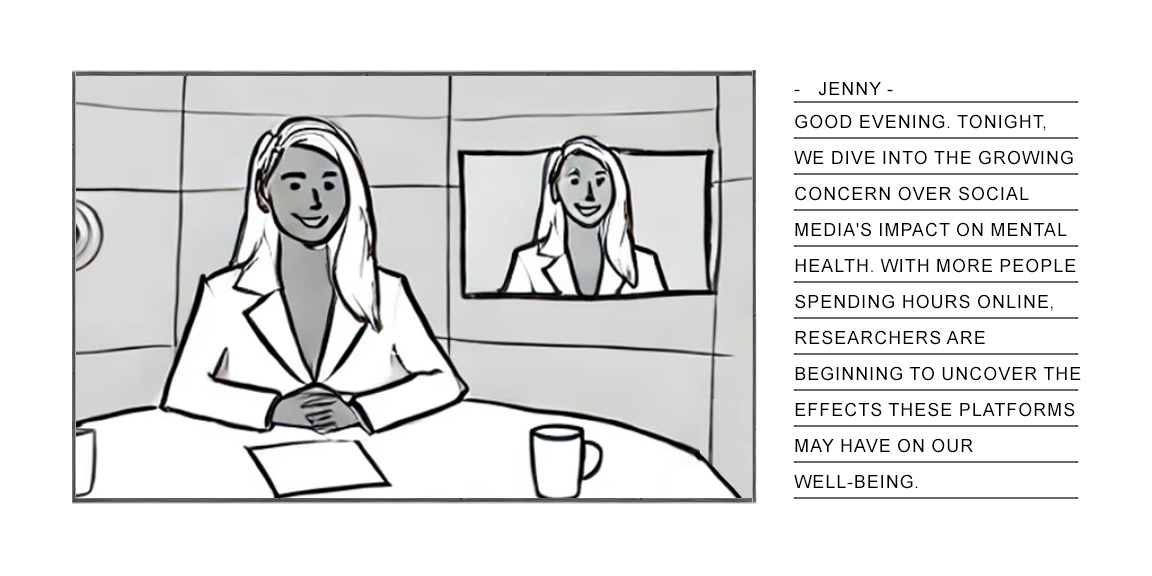
\includegraphics[width=1\linewidth,height=\textheight,keepaspectratio]{images/storyboard-script.jpg}
\caption{Example of a storyboard with script}
\end{figure}

\subsubsection*{Structuring the Storyboard}\label{structuring-the-storyboard}
\addcontentsline{toc}{subsubsection}{Structuring the Storyboard}

The structure of the storyboard should mirror the structure of the script, with panels created for each scene or segment of the broadcast. Each panel should include a rough sketch of the visual, a description of the shot, and the corresponding lines from the script. This helps to ensure that the visuals and the spoken content are closely aligned, creating a cohesive narrative that is both engaging and easy to follow. The panel layout should be detailed enough to guide the production process but flexible enough to allow for adjustments as needed.

Timing and pacing are critical considerations in the storyboard. Each scene should be timed to ensure that the broadcast flows smoothly and maintains the audience's interest. The pacing of the visuals should be aligned with the delivery of the script, with each visual element timed to appear at the most impactful moment. For example, a key graphic might be timed to appear just as the script reaches a critical point, helping to reinforce the message and maintain viewer engagement.

Once the storyboard is complete, it is essential to review and revise it to ensure that it effectively communicates the research findings. This might involve making adjustments to improve clarity, visual appeal, or alignment with the script. The goal is to create a storyboard that not only guides the production process but also enhances the overall impact of the broadcast, ensuring that the research is communicated in a way that is both informative and engaging.

\section{Utilizing Social Media Platforms}\label{utilizing-social-media-platforms}

\subsection*{Strengths and Limitations}\label{strengths-and-limitations}
\addcontentsline{toc}{subsection}{Strengths and Limitations}

In the digital age, social media platforms have revolutionized the way information is disseminated, offering researchers unparalleled opportunities to share their findings with a global audience. Each platform---Twitter, Facebook, LinkedIn, and Instagram---brings unique strengths and limitations to the table, making them suitable for different types of research communication. Understanding these characteristics is essential for effectively leveraging social media to maximize the reach and impact of your research. This analysis provides an in-depth exploration of the major platforms, focusing on how they can be utilized to disseminate research findings, engage with audiences, and foster academic discourse.

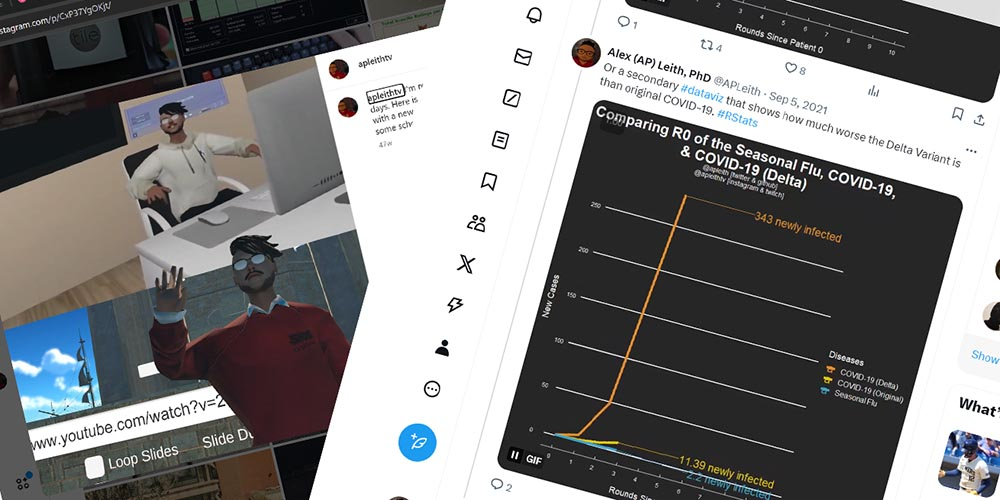
\includegraphics[width=1\linewidth,height=\textheight,keepaspectratio]{images/fig092.jpg}

\subsection*{Twitter}\label{twitter}
\addcontentsline{toc}{subsection}{Twitter}

Twitter stands out as a platform defined by brevity and immediacy, making it an ideal choice for researchers looking to share quick insights and engage in real-time discussions. Its character limit forces users to distill complex ideas into concise, digestible messages, which can be particularly effective for sharing key findings or linking to more detailed content. Twitter's ability to facilitate immediate, real-time engagement is one of its most significant strengths. Researchers can participate in trending conversations, join academic discussions through hashtags like \#AcademicTwitter, and respond to current events or emerging issues relevant to their field. This immediacy not only helps researchers stay connected with their peers but also allows them to contribute to ongoing debates and discussions.

However, the same brevity that makes Twitter accessible can also be a limitation. The platform's character limit may oversimplify complex research findings, reducing nuanced arguments to soundbites. This can be particularly challenging when trying to convey intricate data or theoretical concepts that require more detailed explanations. Additionally, the fast-paced nature of Twitter means that content can quickly become buried under new posts. Trends on Twitter are often fleeting, and important messages can easily get lost in the noise of the platform's constant updates. This volatility can make it difficult for researchers to ensure their content remains visible and engaged with over time.

Despite these challenges, Twitter remains a powerful tool for researchers when used strategically. By crafting concise, impactful messages and using threads to expand on ideas, researchers can effectively communicate their findings and engage with a broad audience. Moreover, the use of visuals such as infographics or videos can complement textual content, enhancing the overall clarity and appeal of the messages shared on Twitter.

\subsection*{Facebook}\label{facebook}
\addcontentsline{toc}{subsection}{Facebook}

Facebook is characterized by its vast and diverse user base, making it a valuable platform for researchers aiming to reach a broad demographic. Unlike Twitter, Facebook supports a variety of content formats, including long-form posts, photos, videos, and links. This versatility allows researchers to provide more detailed explanations of their findings, share full articles, and engage in deeper discussions with their audience. The platform's capacity for multimedia content means that researchers can present their work in a more comprehensive and engaging manner, combining text, visuals, and interactive elements to create a richer user experience.

One of Facebook's key strengths is its ability to reach a wide and varied audience. Researchers can connect with individuals across different age groups, educational backgrounds, and geographic locations, making it a suitable platform for disseminating research to the general public as well as to specialized academic and professional communities. This wide reach can be particularly beneficial for research that has broad societal implications or that seeks to inform public policy.

However, Facebook's algorithmic filtering poses a significant challenge. The visibility of content on Facebook is heavily influenced by its algorithms, which prioritize posts based on user interactions, such as likes, shares, and comments. This can limit the reach of research communications, especially if the content does not generate immediate engagement. Posts may be shown primarily to those within the researcher's immediate network, reducing the potential to reach new audiences outside of this circle. To counteract this, researchers need to create content that is not only informative but also engaging enough to prompt interaction from users, thereby increasing its visibility.

Despite these limitations, Facebook's diverse audience and support for detailed, multimedia-rich posts make it a powerful platform for researchers. By leveraging these strengths and understanding the platform's algorithmic tendencies, researchers can effectively use Facebook to disseminate their work, engage with a wide audience, and foster meaningful discussions about their findings.

\subsection*{LinkedIn}\label{linkedin}
\addcontentsline{toc}{subsection}{LinkedIn}

LinkedIn is distinct among social media platforms for its professional focus, catering primarily to academics, industry experts, and professionals across various fields. This makes it an ideal platform for sharing research that is closely related to industry trends, professional development, or academic advancements. LinkedIn's audience is typically more interested in content that is educational, thought-provoking, and relevant to their professional lives, which aligns well with the dissemination of research findings. The platform also supports the publication of long-form articles and detailed posts, allowing researchers to share in-depth analyses, comprehensive reports, and even case studies.

One of LinkedIn's strengths is the longevity of its content. Unlike Twitter, where posts quickly lose visibility, LinkedIn posts often have a longer lifespan, continuing to receive views, likes, and comments over an extended period. This sustained engagement makes LinkedIn a valuable platform for sharing research that benefits from continued discussion and reflection. Additionally, LinkedIn's professional networking capabilities allow researchers to connect with colleagues, potential collaborators, and industry leaders, facilitating opportunities for collaboration and further dissemination of their work.

However, LinkedIn's focus on professional content can also be a limitation. While it is excellent for reaching a targeted audience of professionals and academics, it may not be as effective for disseminating research to a broader public audience. The platform's niche networking environment means that content is often confined to professional circles, potentially limiting its reach to those interested in diverse research topics outside of their immediate professional interests.

Nevertheless, LinkedIn's strengths in professional networking and content longevity make it an indispensable tool for researchers, particularly when the goal is to connect with peers, share industry-relevant findings, and engage in sustained professional discussions. By tailoring their content to the platform's audience, researchers can effectively use LinkedIn to enhance the visibility and impact of their work within professional and academic communities.

\subsection*{Instagram}\label{instagram}
\addcontentsline{toc}{subsection}{Instagram}

Instagram, known for its visual-centric approach, offers a unique platform for researchers to engage with audiences through creative and visually appealing content. The platform's emphasis on visuals makes it particularly suitable for sharing research findings that can be effectively communicated through images, infographics, and short videos. Instagram's user base is predominantly younger, making it an ideal platform for reaching students, early-career professionals, and a broader public interested in visually engaging content.

Instagram's features, such as Stories and Reels, provide dynamic ways to share research narratives and insights in a more informal and engaging manner. These tools allow researchers to break down their findings into bite-sized pieces, which can be more easily consumed and shared by the platform's users. For example, a researcher could use Instagram Stories to share a step-by-step breakdown of their research process, or create a Reel that summarizes key findings in a visually engaging format. The platform's focus on storytelling through visuals aligns well with the need to make research accessible and engaging to a wider audience.

However, Instagram's strong emphasis on visual content can also be a limitation for research that relies heavily on textual explanations or detailed data presentations. The platform is not well-suited for long-form content or in-depth discussions, which can restrict the depth of information that can be conveyed. Additionally, the need to create visually appealing content that resonates with Instagram's audience may require skills in graphic design or video production, which not all researchers possess.

Despite these limitations, Instagram offers significant opportunities for researchers who can creatively present their findings in a visual format. By using the platform's features to tell stories, engage with a younger audience, and share visually compelling content, researchers can effectively broaden the reach and impact of their work. Instagram's potential for visual storytelling makes it a valuable tool in the researcher's toolkit, particularly for those looking to connect with a diverse and visually-oriented audience.

\chapter{Developing Research Questions and Hypotheses}\label{developing-research-questions-and-hypotheses}

\section{Conceptual Definitions and Operationalization}\label{conceptual-definitions-and-operationalization}

In mass media research, defining and measuring abstract concepts is essential for creating a clear and structured approach to studying communication phenomena. Two critical processes forming this approach's foundation are \textbf{conceptual definition} and \textbf{operationalization}. Understanding these processes allows researchers to build a solid framework for their inquiries, ensuring they accurately capture and analyze the complex elements of media-related phenomena.

\subsection*{Conceptual Definitions}\label{conceptual-definitions}
\addcontentsline{toc}{subsection}{Conceptual Definitions}

A \textbf{concept} is a broad, abstract idea that encapsulates a specific phenomenon researchers want to explore. Concepts act as the foundational building blocks of research, helping scholars focus on particular aspects of media and communication. In mass media research, common concepts include ``media influence,'' ``public opinion,'' and ``audience engagement.'' Each of these concepts represents a broad idea that requires further refinement before it can be effectively studied.

\begin{figure}
\centering
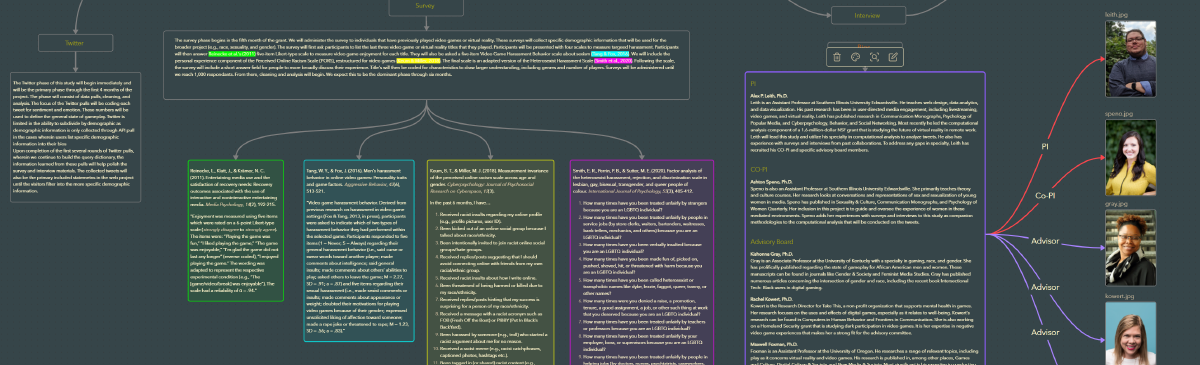
\includegraphics[width=1\linewidth,height=\textheight,keepaspectratio]{images/concept-map.png}
\caption{Example of a concept map during the early stage of project design.}
\end{figure}

For example, take the concept of ``media influence.'' It represents a wide range of possible effects that media could have on individuals or society. These effects might include shaping public opinion, influencing behavior, or reinforcing cultural values. The broad nature of such a concept necessitates clear definition. Researchers need to specify which aspect of media influence they are focusing on to conduct meaningful analysis.

In another example, consider ``audience engagement.'' This concept could refer to various behaviors, such as how audiences consume, interact with, and share media content. Before conducting research on audience engagement, a scholar must define what they mean by the term. Does it refer to passive consumption, like viewing time, or active participation, such as comments and shares on social media? These distinctions are critical because they affect how the concept will be examined and understood.

By narrowing down these broad concepts into specific, clearly defined terms, researchers can target their investigations more effectively. A well-defined concept is crucial for both focusing the scope of a study and ensuring that findings are relevant and actionable.

\subsection*{Operationalization}\label{operationalization}
\addcontentsline{toc}{subsection}{Operationalization}

Once a concept has been clearly defined, the next step is \textbf{operationalization}, which involves transforming abstract concepts into measurable variables. Operationalization bridges the gap between theoretical ideas and empirical research, allowing researchers to gather observable, quantifiable data.

For example, after defining ``audience engagement,'' a researcher must determine how to measure it. Operationalization involves selecting appropriate indicators that accurately reflect the concept. In the case of audience engagement, possible indicators might include metrics like the number of likes, comments, and shares a piece of media content receives. These indicators provide tangible data that can be used to measure audience interaction.

Similarly, if a study focuses on ``media influence,'' operationalization might involve measuring changes in public opinion before and after exposure to a particular media campaign. This could be done through surveys or experiments designed to capture shifts in attitudes or beliefs, allowing researchers to quantify the concept of media influence meaningfully.

Choosing appropriate indicators is crucial to operationalization, as the selected measures must accurately reflect the concept being studied. Poor operationalization can lead to unreliable or invalid results, undermining the overall integrity of the research.

\subsection*{The Importance of Conceptual Definitions and Operationalization}\label{the-importance-of-conceptual-definitions-and-operationalization}
\addcontentsline{toc}{subsection}{The Importance of Conceptual Definitions and Operationalization}

Defining and operationalizing concepts are vital because they form the backbone of any empirical study. Without clear definitions, researchers risk ambiguity, making it difficult to draw valid conclusions from their findings. Similarly, without precise operationalization, measuring abstract ideas in a way that produces reliable and valid data becomes impossible.

Given the complex and often intangible nature of the phenomena studied, these processes are particularly important in mass media research. Concepts like media influence, audience engagement, and public opinion are multifaceted and require careful conceptualization and measurement. By clearly defining their concepts and developing sound operational definitions, researchers ensure their studies are rigorous and meaningful, contributing to a deeper understanding of media processes and effects.

This knowledge is essential for conducting reliable research in mass media, as it ensures that the abstract ideas central to media studies can be systematically examined and understood. Through conceptual definition and operationalization, researchers can turn theoretical ideas into concrete, measurable realities, paving the way for studies that yield insightful and actionable findings.

\section{Identifying Independent and Dependent Variables}\label{identifying-independent-and-dependent-variables}

Understanding independent and dependent variables is fundamental in structuring research, particularly when studying cause-and-effect relationships. These variables are the backbone of empirical research, allowing researchers to manipulate one factor to observe its influence on another. In mass media research, identifying and distinguishing between independent and dependent variables is crucial for defining clear research questions, testing hypotheses, and producing meaningful findings.

\subsection*{Independent Variables}\label{independent-variables}
\addcontentsline{toc}{subsection}{Independent Variables}

The \textbf{independent variable (IV)} is the factor that the researcher manipulates or categorizes to examine its effect on another variable. It represents the ``cause'' in a cause-and-effect relationship. In mass media research, the independent variable is often a media-related factor or characteristic that the researcher changes to observe its impact. For example, in a study exploring the effect of media content on audience engagement, the type of media content---such as news, entertainment, or educational programs---would be the independent variable. The researcher manipulates the content type to examine how it influences the outcome, which is the dependent variable.

To clarify, imagine a study investigating how different advertising formats influence consumer behavior. In this case, the independent variable could be the advertisement format---whether it is a video, banner ad, or social media post. By altering the format, the researcher can observe how these changes affect consumer behavior, such as click-through rates or purchasing decisions. The independent variable is the element you control or modify to determine its impact on the dependent variable.

\begin{figure}
\centering
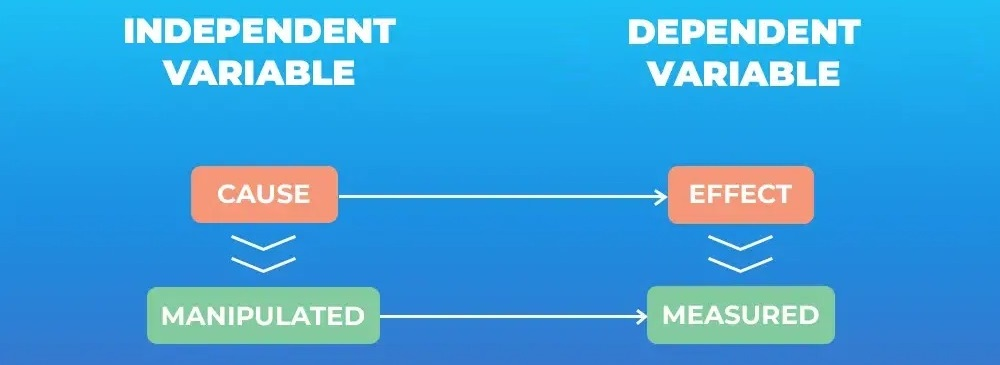
\includegraphics[width=1\linewidth,height=\textheight,keepaspectratio]{images/ind-dep.jpg}
\caption{Difference between Independent and Dependent Variables}
\end{figure}

\subsection*{Dependent Variables}\label{dependent-variables}
\addcontentsline{toc}{subsection}{Dependent Variables}

The \textbf{dependent variable (DV)} is the outcome measured in response to changes in the independent variable. It represents the ``effect'' in the cause-and-effect relationship. The dependent variable is what the researcher observes and records, indicating how the independent variable influences the phenomenon under study.

In mass media research, the dependent variable could be audience behavior, perceptions, or attitudes. For example, in a study measuring the impact of media content on engagement, the dependent variable might be audience engagement. This could be quantified by metrics such as the number of comments, likes, shares, or the time spent viewing the content. The researcher examines these metrics to see if and how they are influenced by changes in the independent variable, such as the type or style of media content presented.

Consider another example: a study exploring the effect of headline styles on readers' perceptions of news credibility. The dependent variable could be the credibility score that participants assign to each article after reading it. By measuring this score, the researcher can assess whether variations in the headline (the independent variable) have a measurable impact on how credible readers perceive the news to be.

\subsection*{Cause-and-Effect}\label{cause-and-effect}
\addcontentsline{toc}{subsection}{Cause-and-Effect}

The relationship between independent and dependent variables is essential for understanding how different aspects of media influence behavior, attitudes, or perceptions. For example, if you are studying the effect of social media usage on academic performance, social media usage would be the independent variable. In contrast, academic performance, measured through test scores or grades, would be the dependent variable. In this case, the researcher is investigating whether the amount of time spent on social media influences academic outcomes.

Understanding this relationship allows researchers to test specific hypotheses about media effects. For instance, if you hypothesize that ``increased exposure to political ads leads to higher voter turnout,'' the independent variable is the exposure to political ads, and the dependent variable is voter turnout. By manipulating the independent variable---changing the level of exposure to political ads---you can measure its effect on the dependent variable, voter turnout.

\subsection*{The Role of Variables in Experimental Design}\label{the-role-of-variables-in-experimental-design}
\addcontentsline{toc}{subsection}{The Role of Variables in Experimental Design}

Correctly identifying independent and dependent variables is crucial for designing experiments and interpreting results in mass media research. Independent variables allow researchers to explore different media formats, messages, or platforms, while dependent variables help measure the outcomes of those explorations. This structured approach provides insights into the effects of media on individuals and society.

For instance, a researcher investigating how different frequencies of advertisement exposure affect brand recall must clearly define the independent variable (frequency of advertisement exposure) and the dependent variable (brand recall). Understanding these variables enables the researcher to design an experiment that tests specific hypotheses, yielding actionable insights about advertising strategies and their effectiveness.

By mastering the identification of independent and dependent variables, you can design robust studies that accurately test your hypotheses, contribute to mass media research, and offer meaningful conclusions. This knowledge is critical for conducting your research and evaluating the work of others, allowing you to critically assess the validity and reliability of existing studies in the academic literature.

\section{Formulating Research Questions}\label{formulating-research-questions}

A well-formulated research question is the foundation of any successful research study. In mass media research, the research question defines the focus and scope of your study, guiding both the theoretical framework and methodological approach. It sets the stage for hypothesis development, data collection, and analysis, ensuring the study remains focused and relevant.

Research questions serve as the guiding force behind your inquiry. They narrow broad topics into specific areas that can be explored systematically, allowing you to investigate particular aspects of media, communication, or social phenomena. Crafting a strong research question is an essential skill for any researcher, as it determines the direction and clarity of the entire study.

\subsection*{What Makes a Good Research Question?}\label{what-makes-a-good-research-question}
\addcontentsline{toc}{subsection}{What Makes a Good Research Question?}

A \textbf{good research question} should be clear, focused, and researchable. It should be specific enough to guide your study but broad enough for comprehensive exploration. In mass media research, the question should focus on a particular media-related phenomenon, effect, or relationship that can be empirically investigated.

For example, consider a broad topic like ``media influence.'' This is too vague to form a research question. However, by refining this idea, we can develop a more focused question: ``How does exposure to political news on social media affect young adults' trust in traditional news outlets?'' This question is specific, measurable, and directly related to a phenomenon that can be empirically tested.

A strong research question should also align with your research objectives. It should be framed in a way that reflects what you aim to discover or explain through your study. This helps ensure that your research remains coherent and that your findings are relevant to the broader field of mass media studies.

\subsection*{Types of Research Questions}\label{types-of-research-questions}
\addcontentsline{toc}{subsection}{Types of Research Questions}

Several types of research questions can be used in mass media research, depending on the goals of your study:

\begin{enumerate}
\def\labelenumi{\arabic{enumi}.}
\item
  \textbf{Descriptive Questions}: These questions describe a particular phenomenon's characteristics or features. For instance, ``What types of content do people engage with most on social media platforms?'' is a descriptive question because it aims to outline patterns or trends without exploring underlying causes.
\item
  \textbf{Comparative Questions}: These questions compare two or more groups, media forms, or phenomena. An example might be, ``How do perceptions of news credibility differ between users of traditional news media and social media?''
\item
  \textbf{Causal Questions}: These questions investigate the cause-and-effect relationships between variables. For example, ``Does exposure to violent video games increase aggressive behavior among adolescents?'' explores a potential causal relationship between media exposure and behavioral outcomes.
\item
  \textbf{Correlational Questions}: These questions examine the relationships between variables without implying causation. An example would be, ``Is there a correlation between social media usage and levels of political participation among young adults?''
\item
  \textbf{Exploratory Questions}: These questions are used when a topic is relatively new or underexplored. For instance, ``How do virtual influencers impact audience perceptions of authenticity in digital marketing?'' explores a contemporary issue with less established research.
\end{enumerate}

\subsection*{The Process of Developing a Research Question}\label{the-process-of-developing-a-research-question}
\addcontentsline{toc}{subsection}{The Process of Developing a Research Question}

Developing a research question begins with identifying a broad area of interest within the field of mass media. From there, you narrow down your focus to a specific topic that is both relevant and researchable. The key is to strike a balance between being too broad, which can make your study unwieldy, and too narrow, which may limit the scope and significance of your findings.

Here's a step-by-step approach to developing a research question:

\begin{enumerate}
\def\labelenumi{\arabic{enumi}.}
\item
  \textbf{Identify a General Topic}: Start with a broad area of interest within mass media, such as ``social media influence'' or ``news consumption patterns.''
\item
  \textbf{Conduct a Literature Review}: Review existing studies to understand what research has already been done on your topic. This will help you identify gaps in the literature that your study can address.
\item
  \textbf{Refine the Topic}: Based on your literature review, narrow your focus to a specific aspect of the topic. For example, instead of studying ``social media influence'' broadly, you might focus on ``the effects of social media on political engagement among young adults.''
\item
  \textbf{Formulate the Question}: Turn your refined topic into a clear, specific research question. For instance, ``How does social media usage influence political engagement among young adults during election campaigns?''
\item
  \textbf{Evaluate the Question}: Ensure your question is clear, focused, and feasible. Ask yourself if it can be answered through empirical research and if it aligns with your study's objectives.
\end{enumerate}

\subsection*{The Importance of Well-Defined Research Questions}\label{the-importance-of-well-defined-research-questions}
\addcontentsline{toc}{subsection}{The Importance of Well-Defined Research Questions}

A well-defined research question is crucial because it sets the parameters for your entire study. It informs the selection of your research methods, the design of your study, and the interpretation of your results. Without a clear question, research risks becoming unfocused, leading to ambiguous findings that may not contribute meaningfully to the field.

In mass media research, where the phenomena studied are often complex and multifaceted, a precise research question ensures that your study targets specific elements that can be measured and analyzed. For instance, a broad question like ``How does media influence society?'' is difficult to address due to its vagueness. In contrast, a specific question like ``How does exposure to negative political advertisements affect voter turnout among first-time voters?'' is focused and measurable, allowing for a more structured and insightful investigation.

By developing strong research questions, you enhance the clarity and focus of your study and contribute to the overall rigor of your research. A well-constructed research question leads to clear, actionable insights, ultimately advancing mass media research and deepening our understanding of the relationships between media, society, and communication.

Through carefully formulating research questions, you will be equipped to design studies that address key issues in media research, paving the way for hypotheses that can be systematically tested and analyzed.

\section{Constructing Hypotheses}\label{constructing-hypotheses}

In mass media research, constructing hypotheses is a critical step that allows researchers to test specific ideas and examine relationships between variables. Hypotheses structure your study, ensuring that the research is systematic and focused. When formulated correctly, hypotheses guide the collection and analysis of data, leading to sound, evidence-based conclusions.

Three key components are involved in hypothesis construction: the \textbf{null hypothesis (H0)}, the \textbf{alternative hypothesis (H1)}, and the \textbf{research question}. Each serves a unique function in the research process, helping to frame the study and focus the inquiry.

\subsection*{Null Hypothesis (H0)}\label{null-hypothesis-h0}
\addcontentsline{toc}{subsection}{Null Hypothesis (H0)}

The \textbf{null hypothesis (H0)} posits that there is no effect or no relationship between the variables under investigation. It serves as a starting point for your research, functioning as a baseline that your study aims to test. The null hypothesis is essential because it provides a clear, falsifiable statement that can be supported or rejected based on empirical evidence.

For example, consider a study examining the impact of media consumption on political attitudes. The null hypothesis might be: ``There is no difference in political attitudes between individuals who consume a high amount of media and those who consume a low amount.'' This hypothesis assumes that media consumption has no measurable effect on political attitudes. Your research aims to determine whether the data supports or refutes this assumption.

By beginning with the null hypothesis, researchers can remain objective in their approach. It creates a framework in which the data, rather than assumptions or biases, determines the outcome. If sufficient evidence is found to reject the null hypothesis, it suggests that a relationship or effect exists between the variables.

\begin{figure}
\centering
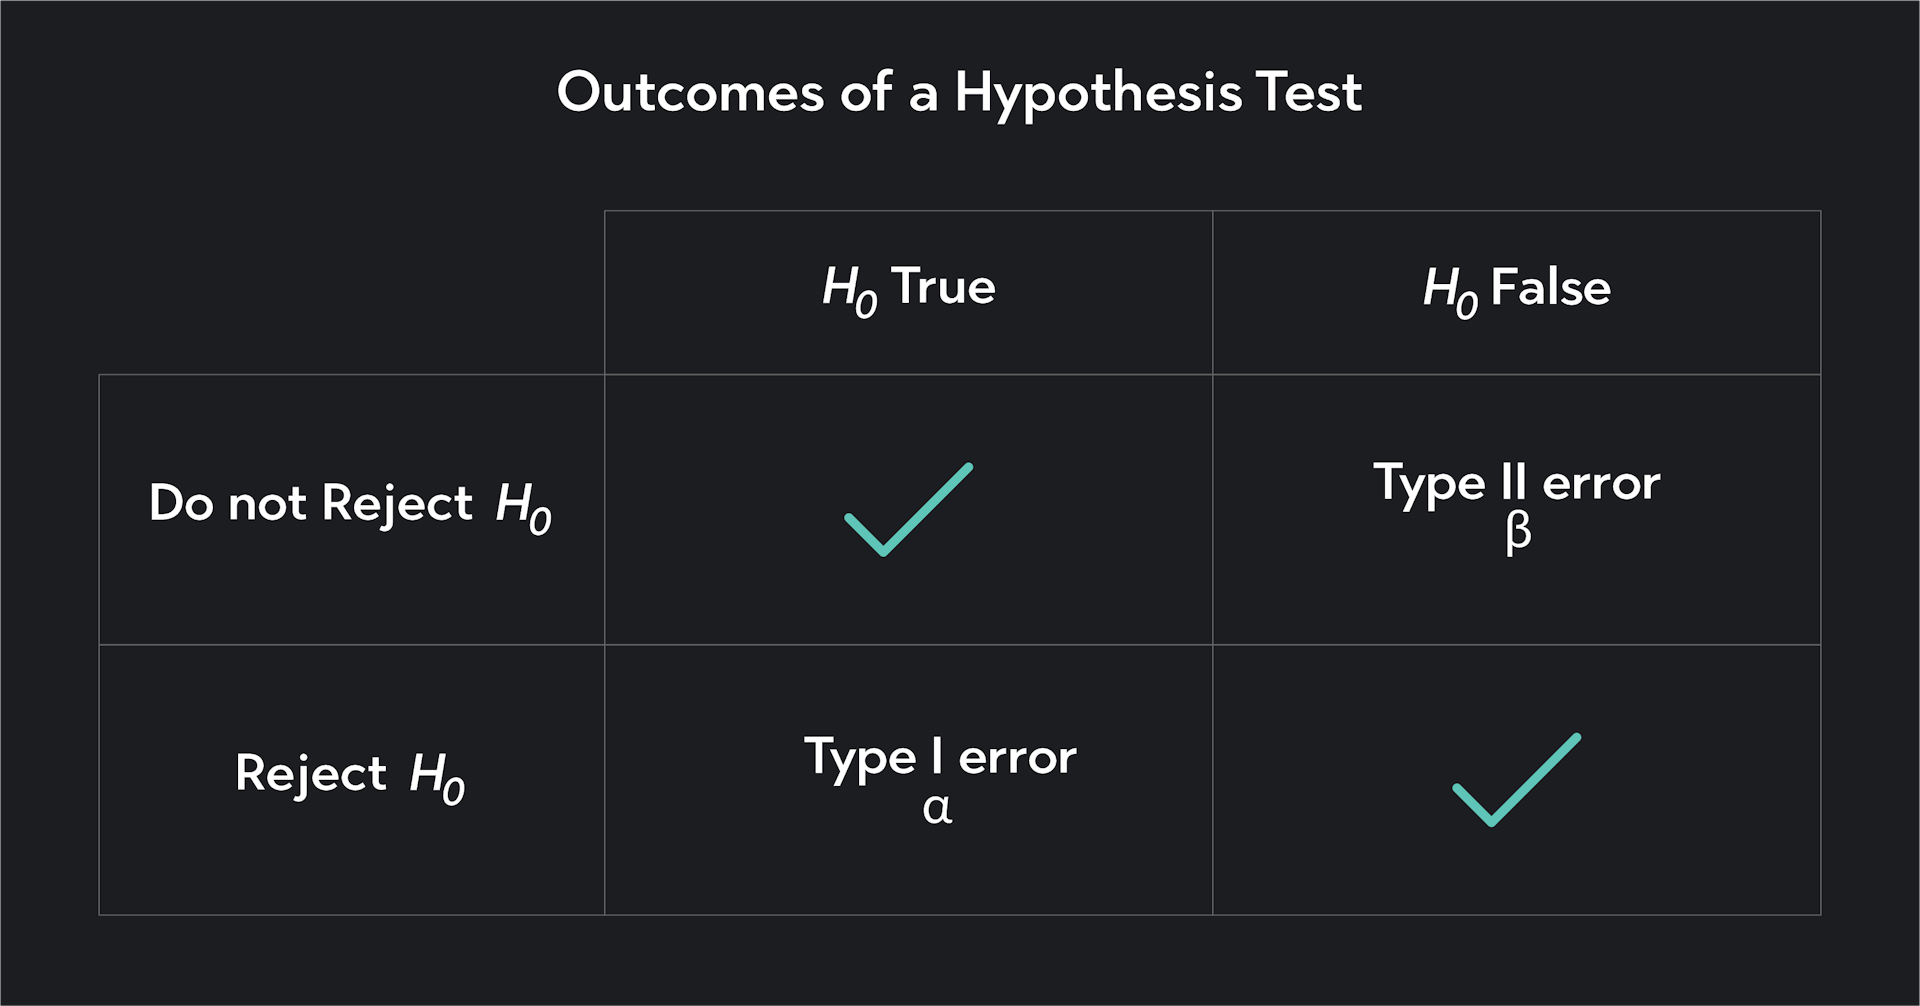
\includegraphics[width=1\linewidth,height=\textheight,keepaspectratio]{images/h0-ha.png}
\caption{Type Errors and Hypotheses}
\end{figure}

\subsection*{Alternative Hypothesis (H1)}\label{alternative-hypothesis-h1}
\addcontentsline{toc}{subsection}{Alternative Hypothesis (H1)}

In contrast to the null hypothesis, the \textbf{alternative hypothesis (H1)} asserts that there is a relationship or effect between the variables being studied. The alternative hypothesis directly opposes the null hypothesis, proposing that some change, difference, or relationship is present.

Continuing with the previous example, the alternative hypothesis might state: ``Individuals who consume a high amount of media have different political attitudes than those who consume a low amount.'' This hypothesis suggests that media consumption influences political attitudes. Your research will then gather evidence to support or refute this claim.

The alternative hypothesis is the hypothesis you are actively testing. It reflects your expectations about the relationship between variables and is usually derived from existing theory or literature. However, the evidence must show that the observed effects or relationships are statistically significant to accept the alternative hypothesis.

\subsection*{The Role of Hypotheses in Research Design}\label{the-role-of-hypotheses-in-research-design}
\addcontentsline{toc}{subsection}{The Role of Hypotheses in Research Design}

Constructing hypotheses is a central part of research design because it determines what to test and how to measure the relationships between variables. Hypotheses provide structure, helping researchers clarify their focus and ensure that their studies are methodologically sound.

In mass media research, hypotheses often explore how different forms of media affect behavior, attitudes, or social outcomes. For instance, a study may hypothesize that exposure to violent video games increases aggressive behavior in teenagers, or that social media usage is positively correlated with levels of political engagement. These hypotheses help frame the research question to allow for measurable outcomes, ensuring that the study can produce actionable insights.

By the end of this section, you should understand how to construct clear, testable hypotheses and formulate research questions that effectively guide your study. Mastering this process will allow you to design rigorous research that contributes valuable knowledge to the field of mass media, helping to explore and clarify the complex relationships between media and society.

\section{Levels of Measurement in Mass Media Research}\label{levels-of-measurement-in-mass-media-research}

Understanding the different levels of measurement is critical to designing sound research and conducting accurate data analysis in mass media studies. The level of measurement determines how data can be categorized, compared, and analyzed, influencing the types of statistical techniques you can apply. There are four primary levels of measurement: \textbf{nominal}, \textbf{ordinal}, \textbf{interval}, and \textbf{ratio}. Each offers a unique approach to organizing and quantifying data, and recognizing these distinctions is essential for conducting effective and meaningful research.

\subsection*{Nominal Level of Measurement}\label{nominal-level-of-measurement}
\addcontentsline{toc}{subsection}{Nominal Level of Measurement}

The \textbf{nominal level} involves classifying data into distinct categories that are mutually exclusive and lack any inherent order. Nominal data groups items based on shared characteristics, without implying any ranking or quantitative value. In mass media research, an example of nominal data could be classifying media content into genres, such as drama, comedy, or documentary. Each genre represents a category, but these categories cannot be ordered or ranked; they are simply different types.

Nominal data is useful for distinguishing between different media types or behaviors, allowing researchers to count occurrences and frequencies within each category. For example, you might count how many television shows fall into each genre. However, because nominal data does not involve any numerical value or rank, mathematical operations such as addition or subtraction are not applicable. Nominal data is foundational for classification purposes, but its limitations mean that more advanced analyses are often impossible at this level.

\subsection*{Ordinal Level of Measurement}\label{ordinal-level-of-measurement}
\addcontentsline{toc}{subsection}{Ordinal Level of Measurement}

The \textbf{ordinal level} introduces an element of order or ranking among categories. Ordinal data allows researchers to rank data points based on relative positions, but the intervals between these ranks are not necessarily consistent or meaningful. For example, a survey asking respondents to rank their preferred social media platforms from most to least preferred produces ordinal data. While this data shows the order of preferences, it does not indicate how much more one platform is preferred over another.

Ordinal data is frequently used in media research to measure preferences, satisfaction, or perceptions. However, because the distances between rankings are unequal, you cannot assume that the difference between first and second place is the same as between second and third. This limitation affects the types of statistical analyses that can be applied, making it essential to use ordinal data appropriately, particularly in studies involving subjective rankings or preferences.

\begin{figure}
\centering
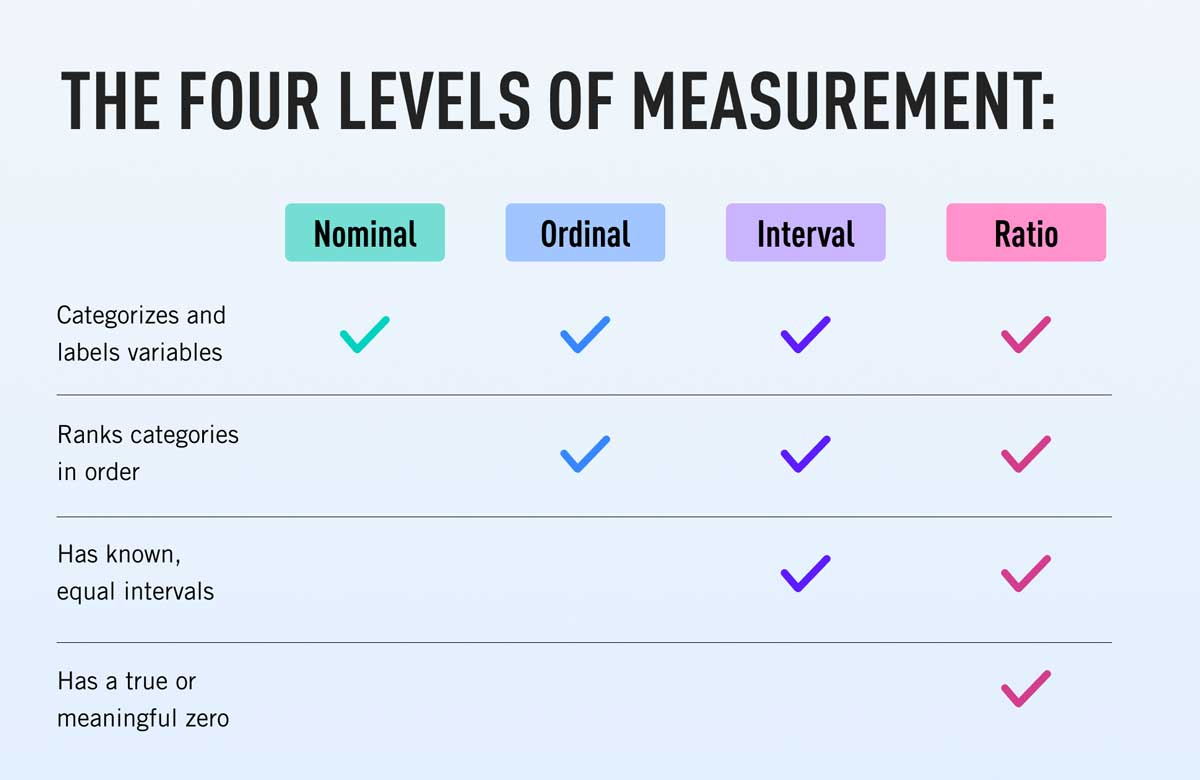
\includegraphics[width=1\linewidth,height=\textheight,keepaspectratio]{images/levels.jpg}
\caption{Levels of Measurement}
\end{figure}

\subsection*{Interval Level of Measurement}\label{interval-level-of-measurement}
\addcontentsline{toc}{subsection}{Interval Level of Measurement}

The \textbf{interval level} of measurement includes data with consistent intervals between values but lacks a true zero point. This means that while you can measure the differences between data points, the data does not allow for statements about absolute quantities. An example of interval data in media research is using a Likert scale, often employed in surveys to measure attitudes or opinions. On a scale from 1 to 5, where 1 represents strong disagreement, and 5 represents a strong agreement, the intervals between each point are equal, but there is no true zero---meaning that a score of 0 does not exist or represent ``no attitude.''

Interval data is particularly valuable in media studies when researchers aim to measure perceptions, attitudes, or responses with precision. Because the intervals between values are equal, you can calculate the mean or standard deviation of responses, which allows for more sophisticated statistical analysis than nominal or ordinal data. However, because interval data lacks a true zero point, it is important to avoid making statements about ratios or absolute quantities. For instance, you cannot say that a score of 4 on a Likert scale is ``twice as positive'' as a score of 2.

\subsection*{Ratio Level of Measurement}\label{ratio-level-of-measurement}
\addcontentsline{toc}{subsection}{Ratio Level of Measurement}

The \textbf{ratio level} of measurement is the most informative and precise, combining all the properties of the interval level with the addition of a true zero point. A true zero indicates the absence of the phenomenon being measured, allowing for meaningful statements about both absolute quantities and ratios. In mass media research, an example of ratio data could be the number of hours spent watching television per week. Since zero hours represent the complete absence of TV viewing, you can make comparisons such as, ``Person A watches twice as much TV as Person B.''

Ratio data is the most versatile and allows for the broadest range of statistical analyses. Researchers can calculate means, medians, variances, and ratios, providing a comprehensive understanding of the data. Ratio data is essential for studies that require precise measurement and comparison of quantities, such as time spent on media platforms, number of social media interactions, or advertising expenditures.

\section{Issues in Measurement}\label{issues-in-measurement}

Accurate and consistent measurement is critical to producing meaningful results in mass media research. However, several challenges can arise during the measurement process that can compromise the integrity of your findings. Among the most significant issues are \textbf{measurement error}, \textbf{validity}, and \textbf{reliability}. Understanding these concepts is essential for designing research that yields accurate and credible data.

\subsection*{Measurement Error}\label{measurement-error}
\addcontentsline{toc}{subsection}{Measurement Error}

\textbf{Measurement error} occurs when there is a discrepancy between the actual value of what is being measured and the observed value. This error can arise from various sources, and even minor inaccuracies can significantly affect a study's outcomes. Common sources of measurement error include respondent misinterpretations, data entry mistakes, and inconsistent data collection methods. For instance, if survey participants misunderstand a question, their answers may not accurately reflect their true thoughts or behaviors, leading to erroneous data. Likewise, the analysis may yield misleading conclusions if data is entered incorrectly into a database.

Consider a study examining the effectiveness of a media literacy program. If participants misunderstand a survey question about their media usage, their responses might not accurately reflect their true habits. This measurement error could skew the results, making it seem as though the media literacy program is more or less effective than it is. Recognizing and minimizing these errors is vital for ensuring the accuracy of research findings.

Minimizing measurement error begins with recognizing its potential sources. Clear, well-designed measurement tools can help reduce misunderstandings, while careful data entry and verification procedures can prevent errors during data processing. Ensuring consistent data collection methods across participants or conditions is equally important in reducing variability that might compromise the study's results.

\subsection*{Validity}\label{validity}
\addcontentsline{toc}{subsection}{Validity}

\textbf{Validity} refers to the extent to which a measurement tool accurately captures the intended concept. If a measurement lacks validity, it may not reflect the true nature of the concept under investigation, leading to incorrect conclusions. In social sciences and media research, \textbf{construct validity} is one of the most critical forms. Construct validity assesses whether the tool or scale genuinely measures the theoretical construct it aims to evaluate.

For example, imagine using a psychological scale in media studies to measure a concept like ``audience engagement.'' To determine whether the scale has strong construct validity, you must evaluate whether the questions truly capture all aspects of audience engagement. If the scale focuses too much on one dimension of engagement---such as how often a user clicks ``like'' on social media posts---while ignoring other important behaviors like commenting or sharing content, its validity would be compromised.

To ensure high construct validity, it's important to design measurement tools based on established theoretical frameworks carefully and to test those tools through pilot studies or existing literature. This process helps researchers verify that their tools accurately measure the concepts they intend to study, leading to more accurate and actionable research findings.

\begin{figure}
\centering
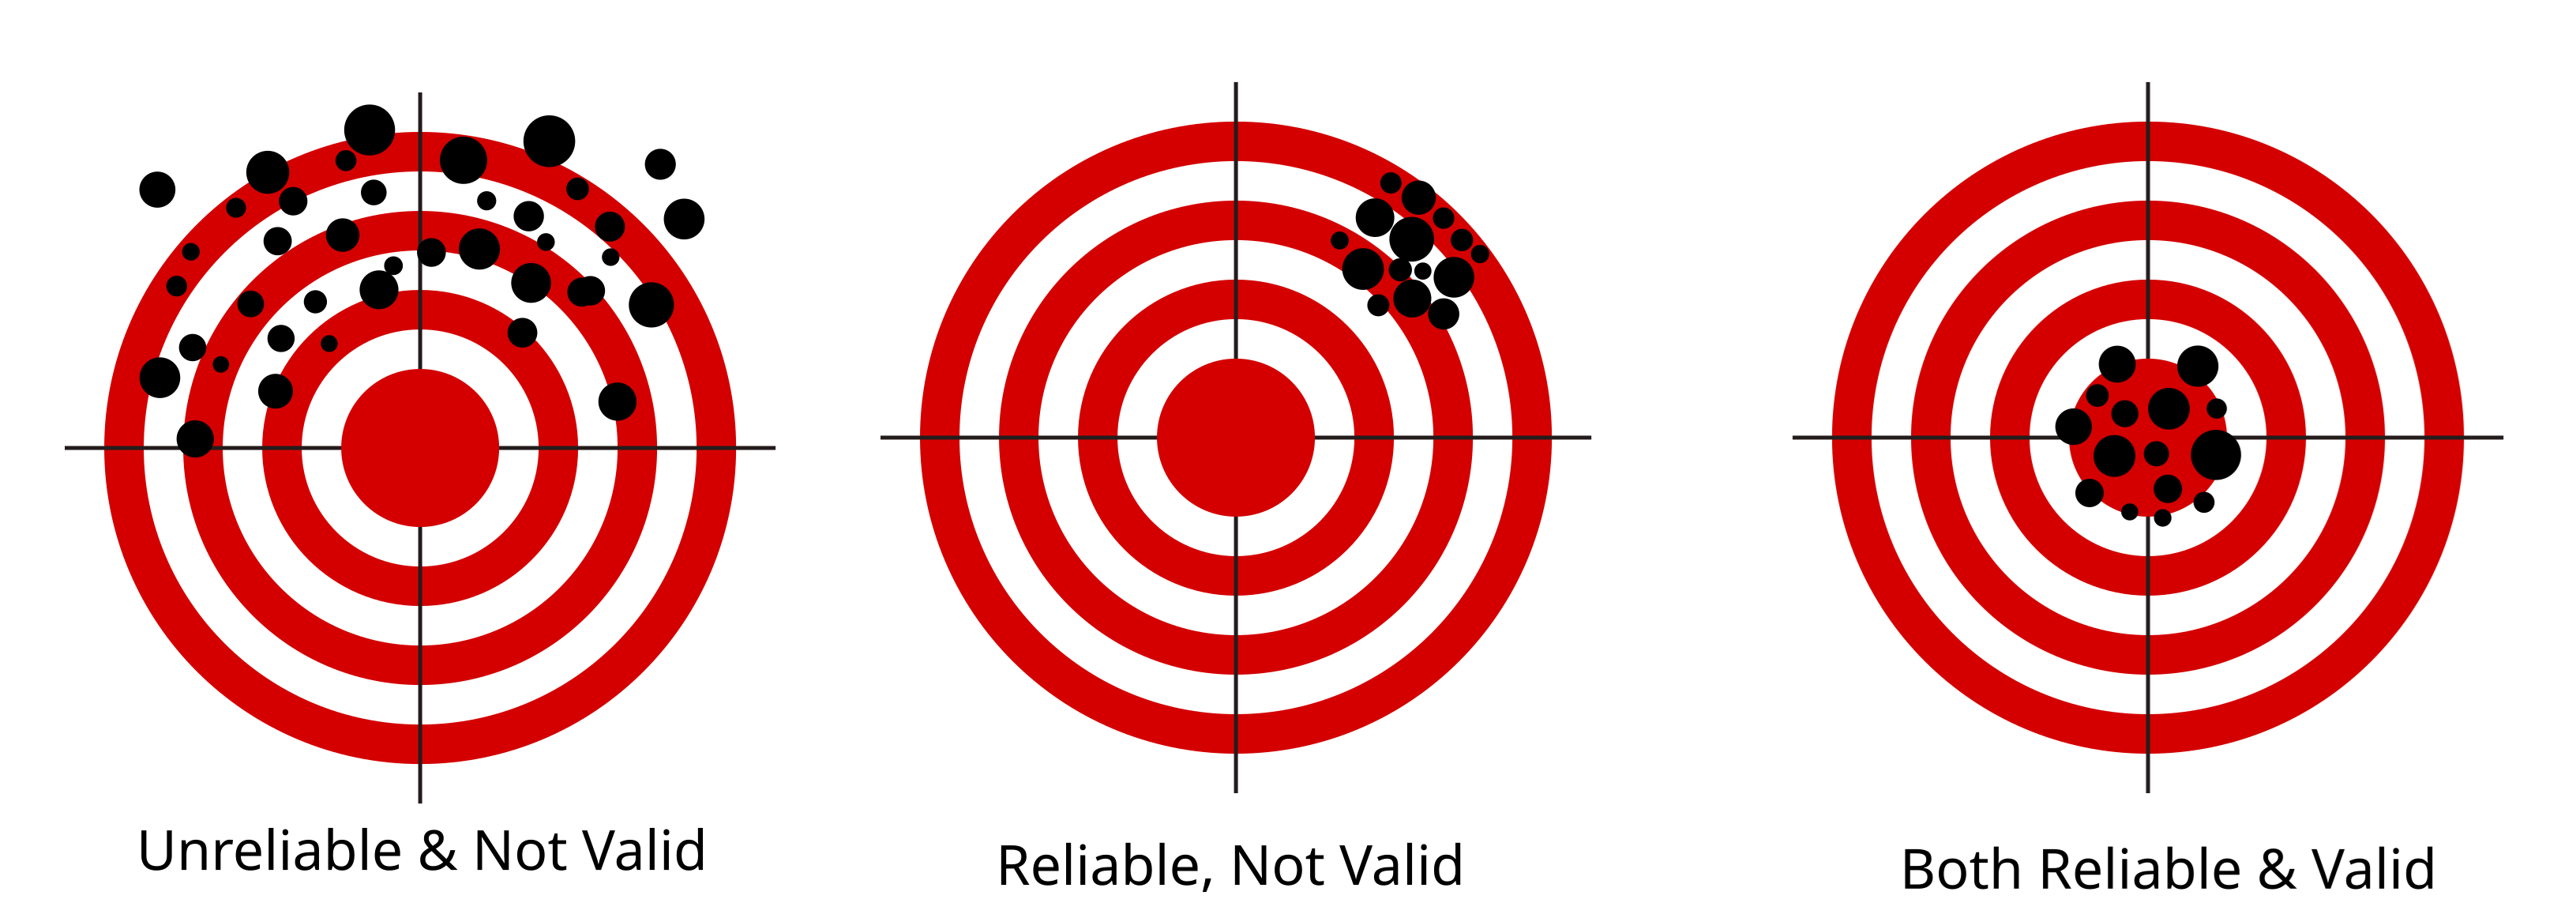
\includegraphics[width=1\linewidth,height=\textheight,keepaspectratio]{images/rel-val.png}
\caption{Reliable vs.~Valid}
\end{figure}

\subsection*{Reliability}\label{reliability}
\addcontentsline{toc}{subsection}{Reliability}

\textbf{Reliability} refers to the consistency of a measurement tool---its ability to produce the same results under the same conditions. A reliable tool will yield similar outcomes each time it is used, assuming that the measured phenomenon remains unchanged. Without reliability, even a valid measurement tool can lead to inconsistent and, thus, untrustworthy results.

For example, if a survey is designed to measure levels of audience engagement but produces vastly different results each time it is administered to the same group under similar conditions, the tool lacks reliability. As a result, it becomes difficult to draw meaningful conclusions from the data because the inconsistency casts doubt on whether the measurements truly reflect audience engagement.

Reliability is critical in mass media research because it ensures that findings are not the product of random fluctuations in measurement but are stable reflections of the studied phenomena. Several methods exist to assess reliability, including test-retest reliability (which evaluates whether the tool yields consistent results over time) and internal consistency (which checks if different parts of the measurement tool produce similar results).

\subsection*{The Relationship Between Validity and Reliability}\label{the-relationship-between-validity-and-reliability}
\addcontentsline{toc}{subsection}{The Relationship Between Validity and Reliability}

Recognizing that validity and reliability are related but distinct concepts is important. A measurement tool must be reliable and valid, as inconsistent results undermine any attempt to measure a construct accurately. However, a reliable tool is not necessarily valid. For instance, a scale might consistently measure something but not the concept it is intended to measure---thus, it is reliable but not valid.

In mass media research, achieving high reliability and high validity is critical to ensuring that your findings accurately reflect your study phenomena. Reliable tools provide stable measurements, while valid tools ensure that you measure the right constructs. Both are essential for producing research that contributes meaningfully to our understanding of media effects, behaviors, and perceptions.

\chapter{Designing Quantitative Research}\label{designing-quantitative-research}

\section{Research Design}\label{research-design}

\subsection*{Experimental Designs}\label{experimental-designs}
\addcontentsline{toc}{subsection}{Experimental Designs}

Experimental designs are a fundamental component of quantitative research in mass media. They offer powerful methods to test hypotheses and establish causal relationships between variables. These designs are beneficial for exploring how different types of media content influence audience behavior and perceptions. By manipulating independent variables and observing the effects on dependent variables, researchers can gain valuable insights into the dynamics of media influence.

\textbf{Between-Subjects Design}

One of the most commonly employed experimental approaches is the \textbf{between-subjects design}. In this design, participants are divided into separate groups, each exposed to a different independent variable level. This structure allows for direct comparisons between groups to determine the effect of varying conditions. For example, one group might watch a news broadcast with a positive tone, while another group views the same one with a negative tone. By measuring differences in audience perceptions between these groups, researchers can assess how the tone of the broadcast affects reception.

The between-subjects design is particularly effective when the goal is to attribute observed effects directly to the independent variable, minimizing the influence of extraneous factors. Since each participant experiences only one condition, there is less risk of biases such as fatigue or learning effects that can occur with repeated exposures. However, ensuring that the groups are equivalent in all respects except for the experimental manipulation is crucial. Random assignment and matching are standard techniques used to achieve group equivalence, thereby enhancing the study's internal validity.

\href{https://www.nngroup.com/articles/between-within-subjects/}{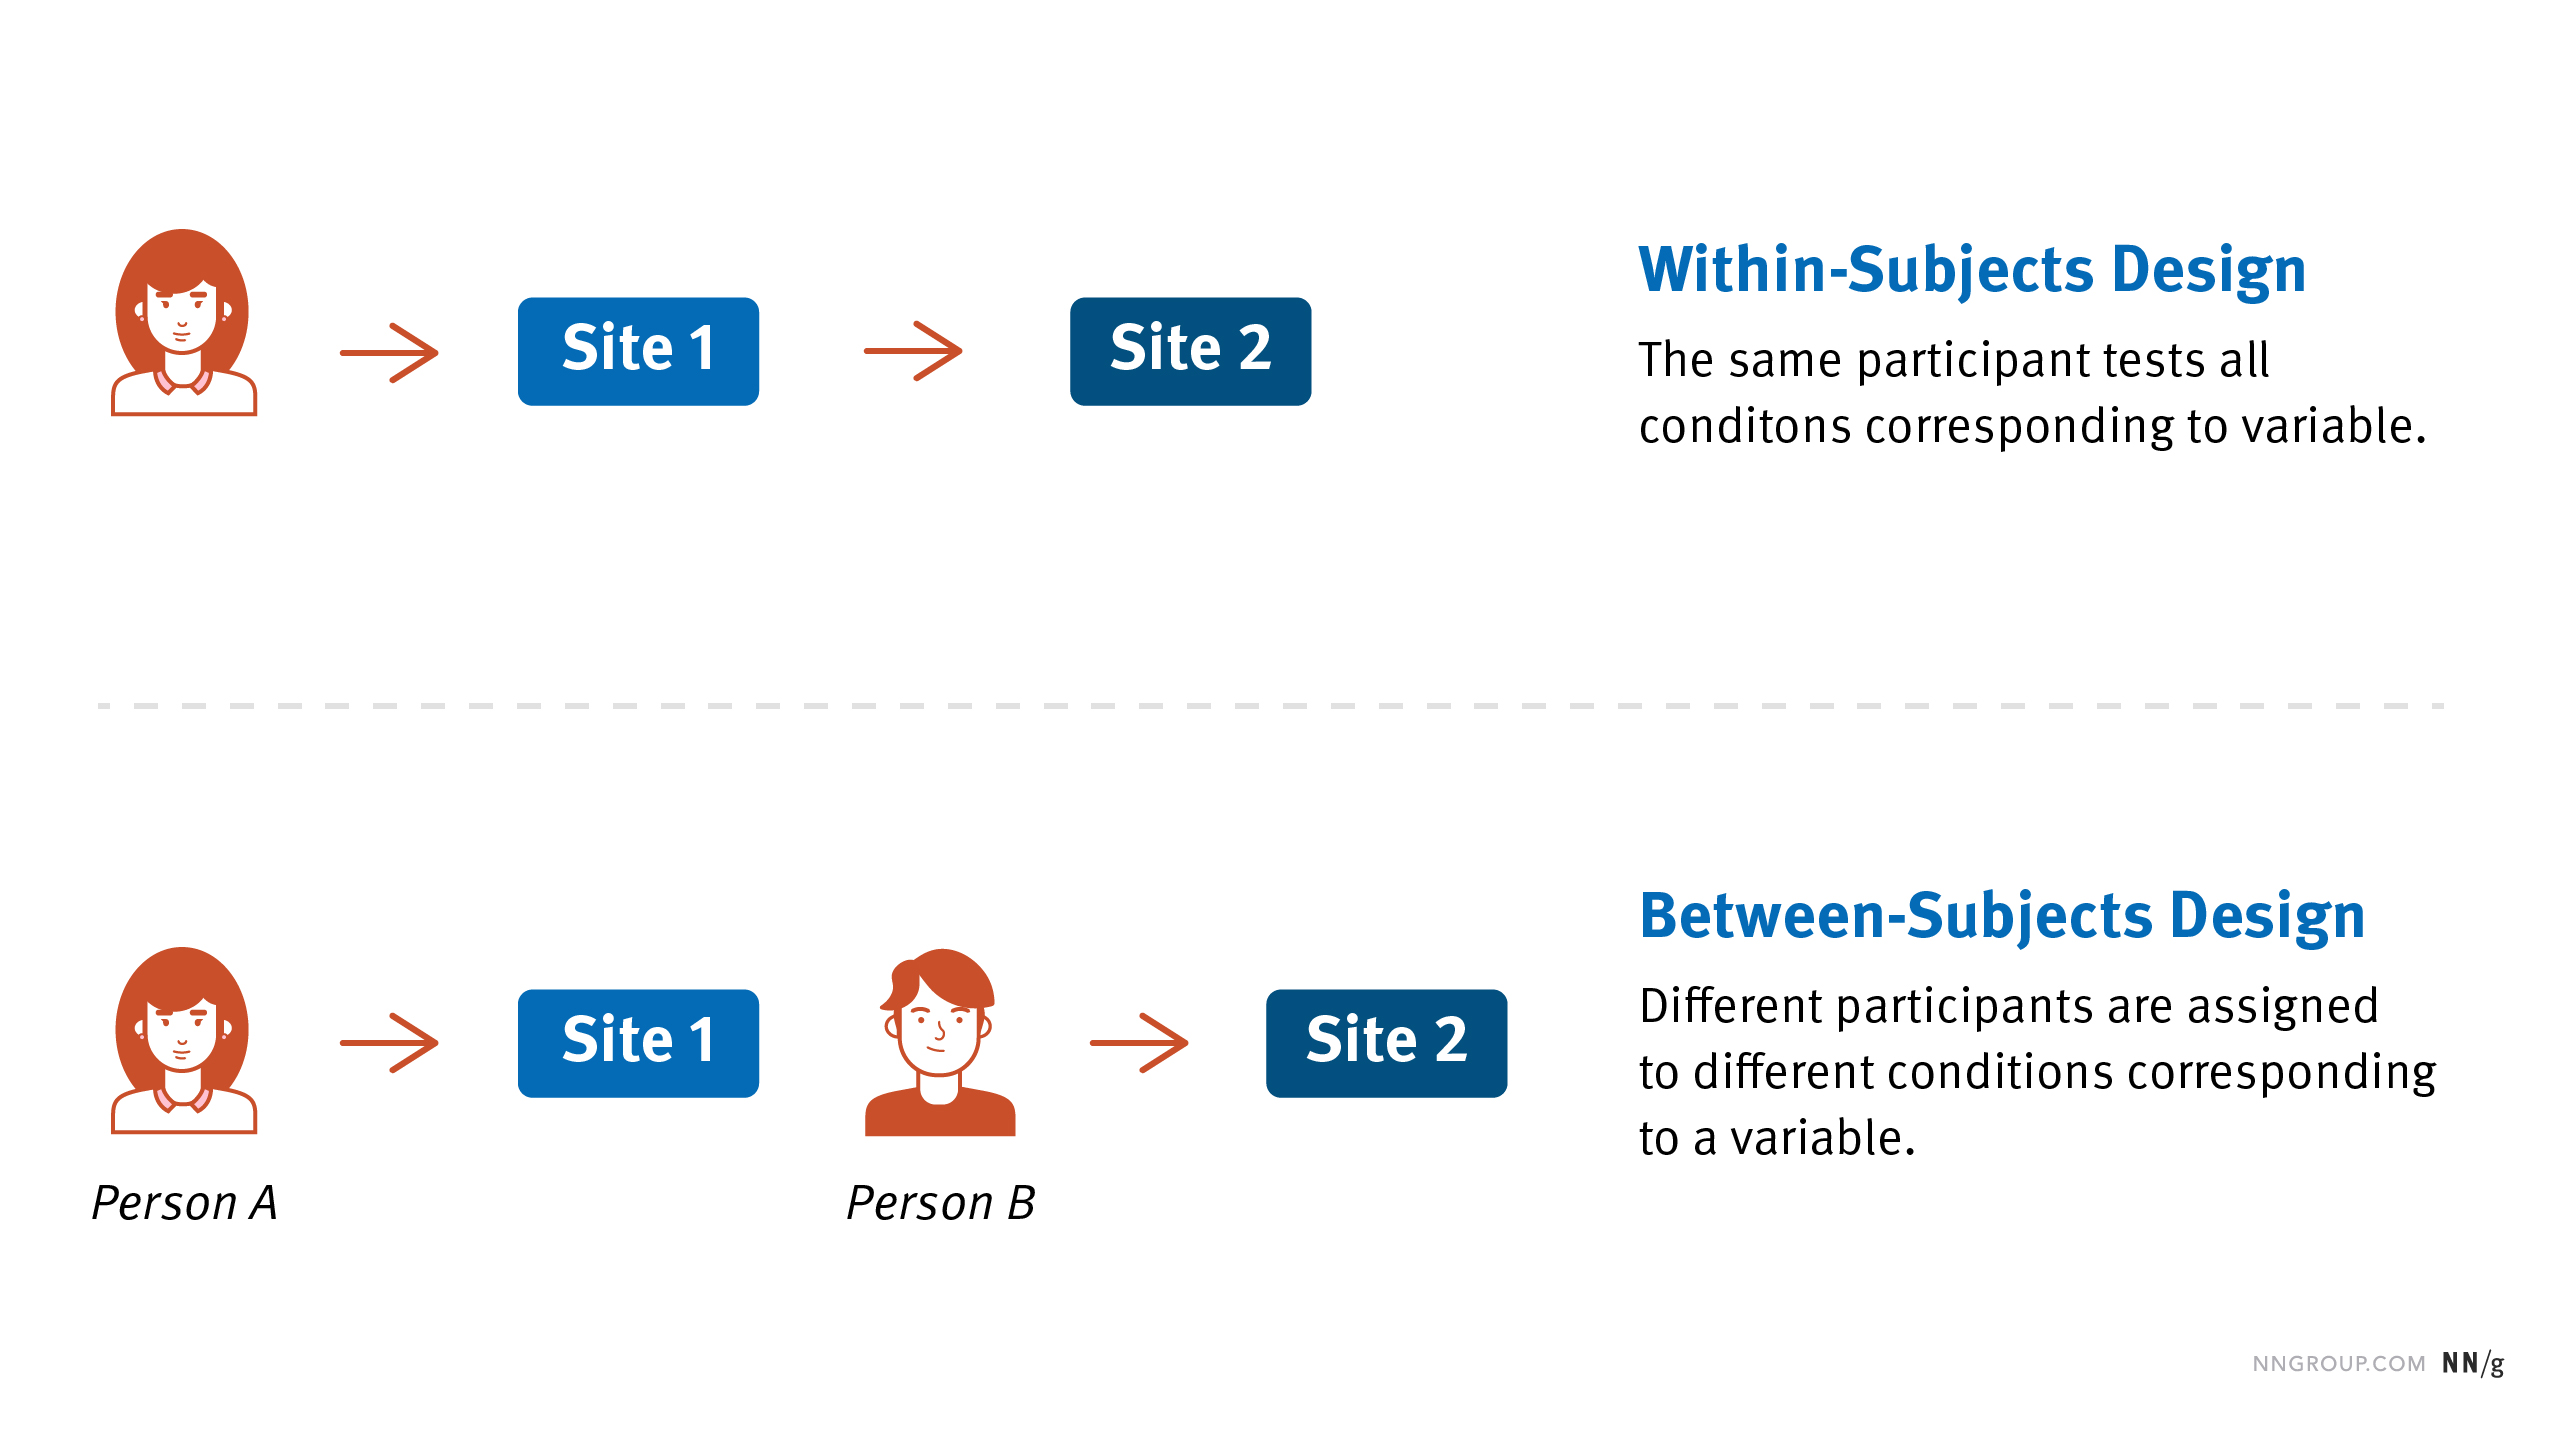
\includegraphics[width=1\linewidth,height=\textheight,keepaspectratio]{images/subject-design-graphic.jpg}}

\textbf{Within-Subjects Design}

In contrast, a \textbf{within-subjects design} involves exposing the same participants to all independent variable levels. This approach allows researchers to observe how changes in the independent variable affect the same individuals, effectively controlling for individual differences. For instance, participants might first watch a news broadcast with a positive tone and later view one with a negative tone, with their reactions measured after each exposure. By comparing responses within the same group, researchers can more precisely determine the impact of the variable.

While within-subjects designs offer the advantage of increased sensitivity to detecting effects, they can also introduce potential issues like order effects. The sequence in which conditions are presented might influence participants' responses due to factors such as fatigue, practice, or carryover effects. To mitigate these concerns, researchers often employ \textbf{counterbalancing} techniques, varying the order of conditions across participants to distribute any order-related influences evenly.

\textbf{Control Groups}

A critical element of any experimental design is including a \textbf{control group}. This group consists of participants who do not receive the experimental treatment and serves as a baseline for comparison. In mass media research, a control group might be exposed to neutral media content, while experimental groups encounter content with specific biases or manipulations. Researchers can determine whether the independent variable has a significant effect by comparing the control group's responses to those of the experimental groups.

Control groups are essential for isolating the impact of the independent variable and ruling out alternative explanations for the findings. Without a control group, it becomes challenging to ascertain whether observed changes are due to the manipulation or other external factors. For example, if both the control and experimental groups exhibit similar changes in perception, this might indicate that factors unrelated to the media content are influencing the results.

\href{https://www.thoughtco.com/control-and-experimental-group-differences-606113}{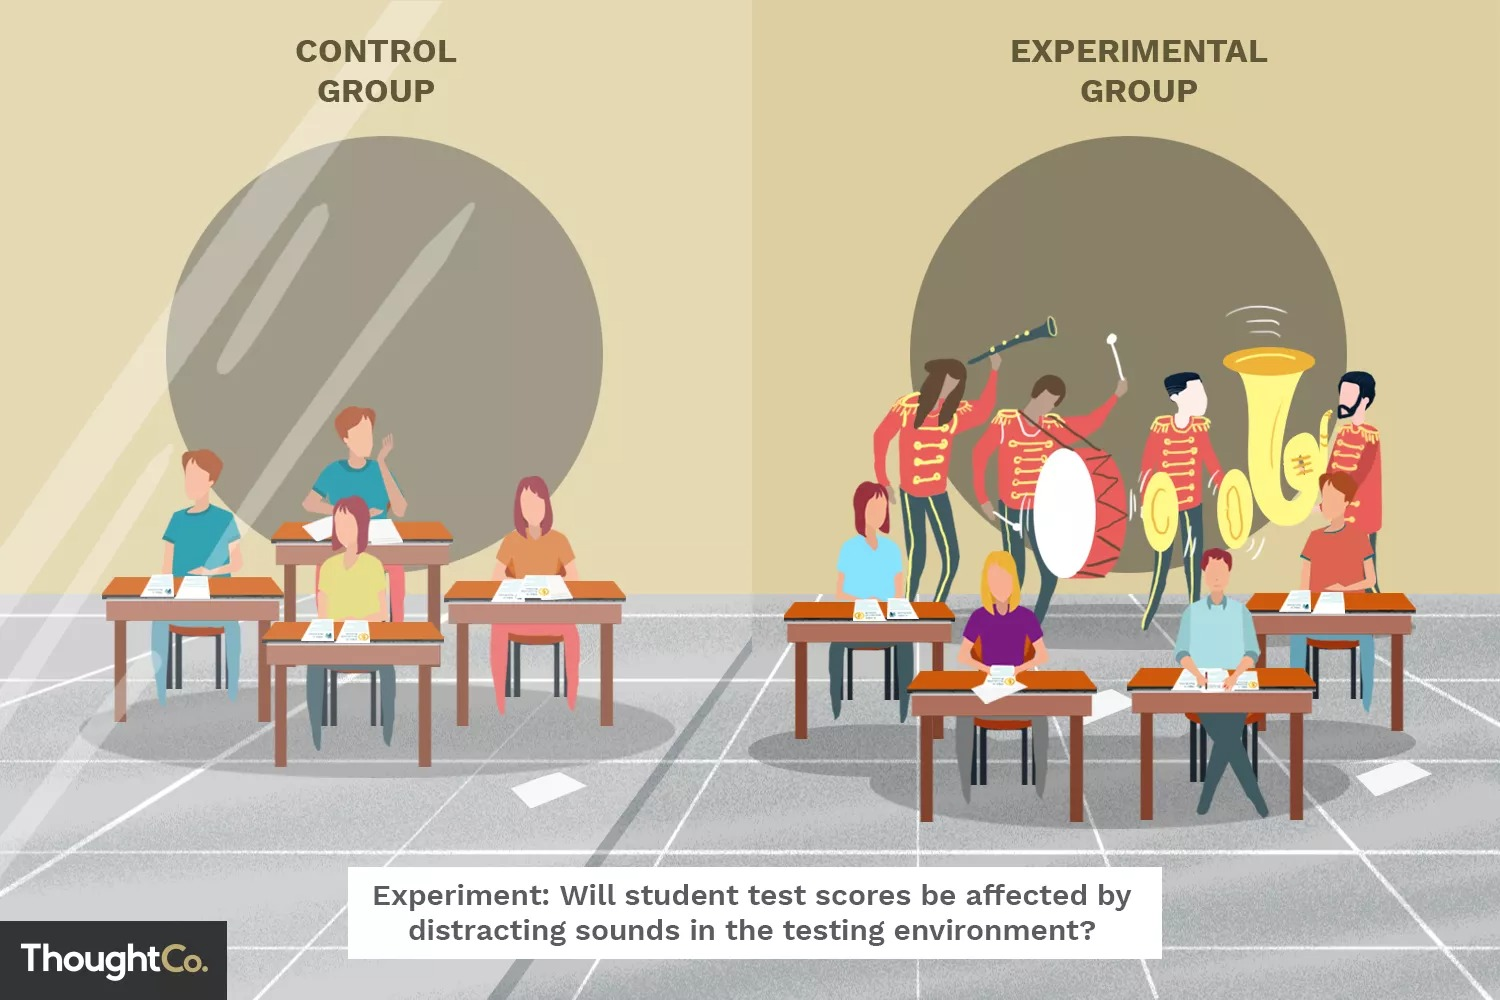
\includegraphics[width=1\linewidth,height=\textheight,keepaspectratio]{images/control.jpg}}

\textbf{Applying Experimental Designs in Mass Media Research}

Understanding how to implement these experimental designs properly is crucial for conducting valid and reliable research in mass media. Through carefully structured experiments, researchers can explore questions such as:

\begin{itemize}
\tightlist
\item
  How does the framing of news stories influence audience attitudes toward social issues?
\item
  What is the effect of exposure to violent media content on aggressive behavior?
\item
  How do different advertising strategies impact consumer purchasing decisions?
\end{itemize}

By selecting the appropriate experimental design, researchers can tailor their studies to effectively address specific research questions. For instance, a between-subjects design might be ideal for comparing the effects of two distinct advertising campaigns on separate groups. Conversely, a within-subjects design could be more suitable for assessing changes in audience perceptions before and after exposure to a particular media message.

\textbf{Conclusion}

Mastering experimental designs empowers researchers to conduct rigorous investigations into the effects of media on audiences. By understanding the strengths and challenges of between-subjects and within-subjects designs, as well as the importance of control groups, researchers can enhance the validity and reliability of their studies. This foundational knowledge is essential for anyone engaged in mass communications research, providing the tools necessary to draw meaningful conclusions about the complex interplay between media content and audience response.

\subsection*{Non-Experimental Designs}\label{non-experimental-designs}
\addcontentsline{toc}{subsection}{Non-Experimental Designs}

In mass media research, not all studies permit experimental manipulation due to ethical, practical, or logistical constraints. In such cases, researchers rely on \textbf{non-experimental designs} to observe and analyze data as it naturally occurs. Two prevalent non-experimental approaches are \textbf{cross-sectional designs} and \textbf{longitudinal designs}. Understanding these methods is essential for conducting meaningful research when experiments are not feasible.

\textbf{Cross-Sectional Designs}

Cross-sectional designs involve observing a specific population at a single point in time. By collecting data simultaneously from different individuals, researchers can identify patterns, trends, and relationships between variables within a population. For example, surveying to assess public opinion on the influence of social media platforms at a particular moment provides a snapshot of current views and behaviors.

The primary advantage of cross-sectional designs is their efficiency. Data collection occurs once, making these studies relatively quick to complete and often less costly than other designs. They are handy for descriptive research aiming to understand the prevalence or distribution of a phenomenon within a population.

However, cross-sectional designs have limitations regarding causal inference. Since data is collected at one point, determining the directionality of relationships between variables or establishing cause-and-effect links is challenging. For instance, if a study finds that individuals who spend more time on social media report higher levels of anxiety, it cannot clarify whether social media use causes anxiety, anxiety leads to increased social media use, or if another factor influences both variables.

\textbf{Longitudinal Designs}

Longitudinal designs involve observing the same participants over an extended period. By tracking changes within the same group of individuals, researchers can more effectively study developments, trends, and potential causal relationships. For example, following a group of participants over several years to examine how prolonged exposure to certain media content influences their political attitudes allows researchers to see how variables evolve and how earlier experiences impact later outcomes.

Longitudinal designs are valuable for studying changes and developments over time. They provide insights into long-term effects and can help establish causality by demonstrating how one variable influences another across different periods. For instance, a longitudinal study might reveal that increased media exposure during adolescence leads to specific changes in political attitudes in adulthood, offering evidence of a causal relationship.

Despite their strengths, longitudinal studies present challenges. Participant attrition, or dropout, is a significant concern. Over time, some participants may leave the study due to loss of interest, relocation, or life changes, which can introduce bias if the remaining participants differ systematically from those who leave. Additionally, longitudinal research is more time-consuming and costly, requiring sustained resources and meticulous planning.

\textbf{Applying Non-Experimental Designs in Mass Media Research}

Understanding the advantages and limitations of cross-sectional and longitudinal designs is crucial for mass media researchers. These designs are often employed when experimental manipulation is not possible, but valuable insights are still needed.

\begin{itemize}
\item
  \textbf{Case Study---Cross-Sectional Design}: A researcher conducts a nationwide survey to explore the relationship between social media usage and trust in traditional news outlets. By analyzing data collected at one point, the researcher identifies correlations and patterns that inform our understanding of media consumption behaviors.
\item
  \textbf{Case Study---Longitudinal Design}: This long-term study follows a group of teenagers over a decade to assess how early exposure to violent video games influences aggressive behavior into adulthood. By collecting data at multiple intervals, the study provides evidence of potential causal links between media exposure and behavioral outcomes.
\end{itemize}

Addressing challenges like participant dropout in longitudinal studies involves maintaining regular contact, offering incentives, and employing tracking methods to keep participants engaged. In cross-sectional studies, careful sampling and statistical controls help mitigate limitations related to causality.

\textbf{Conclusion}

Mastering both cross-sectional and longitudinal designs equips researchers with essential tools for conducting insightful and methodologically sound studies in mass media. While cross-sectional designs offer efficiency and are excellent for identifying current relationships and trends, longitudinal designs provide depth in understanding changes over time and potential causal links. By selecting the appropriate design for specific research questions and being mindful of each approach's strengths and limitations, researchers enhance their findings' validity and impact in the dynamic mass media research field.

\subsection*{Sampling Methods}\label{sampling-methods}
\addcontentsline{toc}{subsection}{Sampling Methods}

The method used to select a sample significantly impacts the validity and generalizability of research findings in mass media studies. \textbf{Sampling methods} determine how participants are chosen from the larger population and are crucial for ensuring that a study accurately represents the intended group. Various sampling methods exist, each with its advantages and limitations. Understanding these methods helps researchers make informed decisions about study design and result interpretation.

\textbf{Random Sampling}

One of the most influential and widely used methods is \textbf{random sampling}. In this approach, participants are selected so that every member of the population has an equal chance of being chosen. Random sampling is considered the gold standard because it minimizes selection bias and enhances the generalizability of study results.

For example, suppose a researcher surveys viewers to understand their preferences for television programs. By randomly selecting viewers from a television network's entire subscriber list, each subscriber---regardless of viewing habits---has an equal chance of inclusion. This randomness helps ensure the sample is representative of the larger population, allowing for more confident generalization of the findings.

Random sampling is particularly valuable when drawing conclusions that apply broadly to the entire population. However, careful planning and sometimes a larger sample size are required to reflect the population's diversity truly. While random sampling reduces bias, it does not eliminate it; factors such as non-response can still introduce some bias.

\begin{figure}
\centering
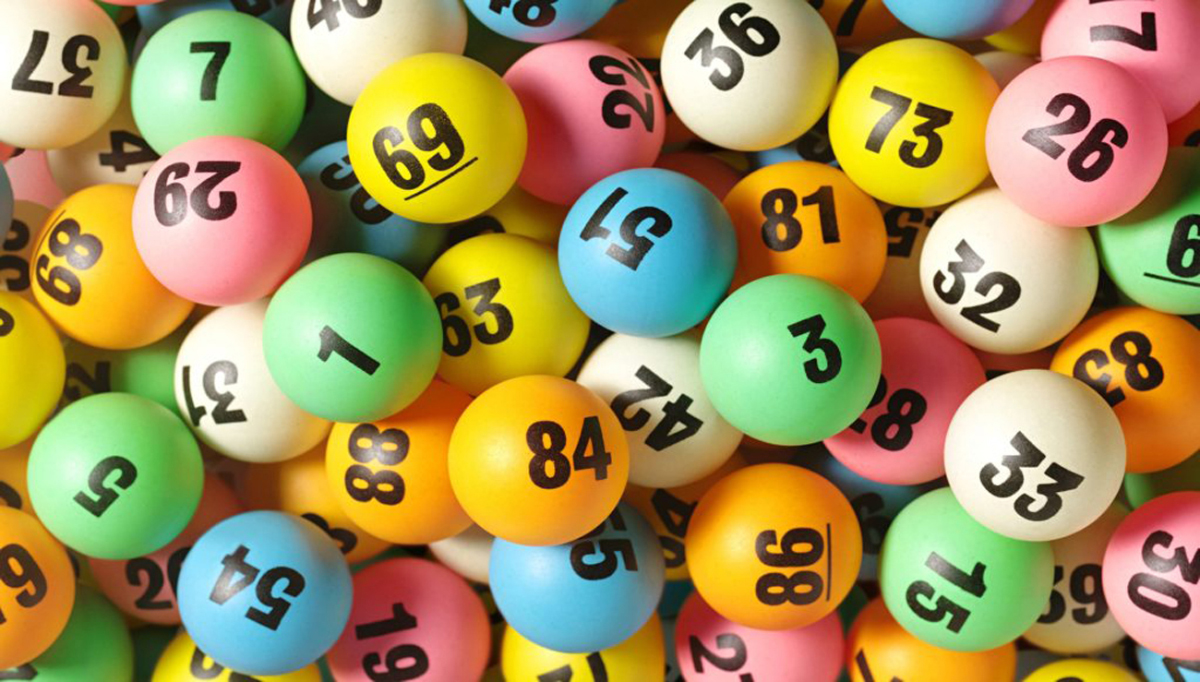
\includegraphics[width=1\linewidth,height=\textheight,keepaspectratio]{images/random.jpg}
\caption{Lottery balls}
\end{figure}

\textbf{Stratified Sampling}

Another critical method is \textbf{stratified sampling}, which involves dividing the population into distinct subgroups or strata and randomly sampling from each group. This approach ensures that each subgroup is adequately represented in the sample, especially when specific characteristics---such as age, gender, or income level---are essential for the research.

For instance, if studying media preferences across different age groups, a researcher might divide the population into age strata (e.g., 18--29, 30--49, 50 and above) and randomly select participants from each group. This method ensures that each age group is proportionally represented, allowing for more precise comparisons between groups.

Stratified sampling is particularly beneficial when the population is heterogeneous, meaning there are significant differences between subgroups. Ensuring proportional representation improves the accuracy of estimates and reduces sampling error. However, it requires detailed knowledge of the population and can be more complex to implement than simple random sampling.

\begin{figure}
\centering
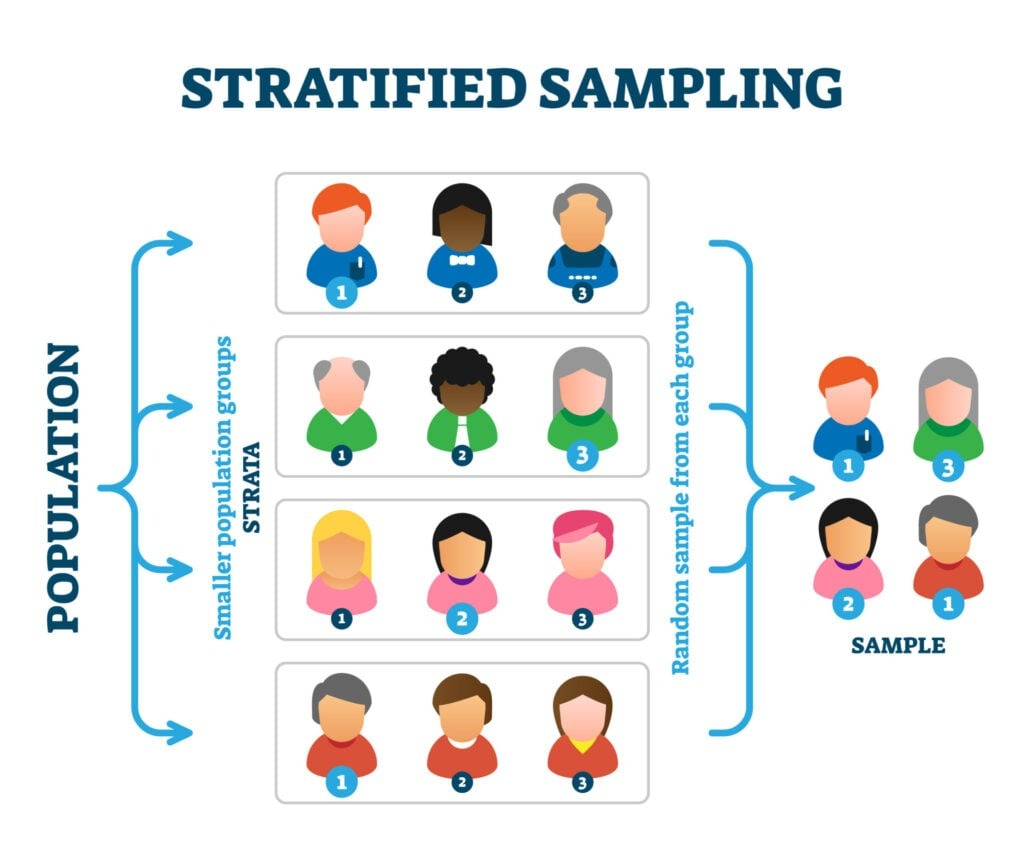
\includegraphics[width=1\linewidth,height=\textheight,keepaspectratio]{images/strata.jpg}
\caption{Representation of stratified sampling}
\end{figure}

\textbf{Convenience Sampling}

In contrast, \textbf{convenience sampling} involves selecting participants who are readily available and accessible to recruit. While practical and cost-effective, this method has significant limitations regarding representativeness and generalizability.

For example, convenience sampling is used to research media habits among college students by surveying students in one's classes. Although straightforward, this sample may not represent all college students or the general population, potentially leading to biases in the findings.

Convenience sampling is often employed in exploratory research, pilot studies, or situations where other methods are not feasible. However, it is crucial to recognize its limitations: since the sample is not randomly selected, results may not be generalizable beyond the specific group studied. To mitigate some drawbacks, researchers can combine convenience sampling with other techniques, such as increasing the sample size or using quota sampling, to ensure some level of diversity within the sample.

\textbf{Applying Sampling Methods in Mass Media Research}

Understanding and correctly applying these sampling methods is vital in mass media research, where accurately capturing audience diversity is essential.

\begin{itemize}
\item
  \textbf{Random Sampling Case Study}: A national survey assessing public trust in news media employs random sampling to include a wide range of demographic groups, enhancing the study's generalizability.
\item
  \textbf{Stratified Sampling Case Study}: A study examining social media usage patterns divides participants into different age groups and samples each subgroup proportionally, ensuring meaningful comparisons across ages.
\item
  \textbf{Convenience Sampling Case Study}: A researcher might survey people at a local shopping mall for a preliminary study on reactions to a new advertising campaign. While offering immediate insights, the findings may not be generalizable to the broader population.
\end{itemize}

\textbf{Conclusion}

By mastering random, stratified, and convenience sampling methods, researchers are better equipped to select the most appropriate approach for their questions and understand each method's implications for their findings. This knowledge is essential for conducting rigorous and credible research in mass media studies, where the sample's representativeness directly affects the results' validity.

\section{Data Collection Techniques}\label{data-collection-techniques}

\subsection*{Surveys and Questionnaires}\label{surveys-and-questionnaires}
\addcontentsline{toc}{subsection}{Surveys and Questionnaires}

Surveys and questionnaires are fundamental tools in mass media research, enabling efficient data collection from many participants. They allow researchers to gather information on attitudes, behaviors, preferences, and other variables of interest. The design of survey questions is critical to ensure that the data collected is accurate, meaningful, and truly reflective of respondents' opinions. Understanding the different types of survey questions---such as Likert-type items, closed-ended and open-ended questions---is essential for designing effective surveys.

\textbf{Likert-Type Items}

One of the most widely used types of survey questions is the \textbf{Likert-type item}. This format presents a statement to which respondents indicate their level of agreement on a scale, typically ranging from ``strongly disagree'' to ``strongly agree.'' For example, a survey might ask respondents to rate their agreement with the statement, ``Social media has a positive impact on society,'' using a scale from 1 (strongly disagree) to 5 (strongly agree). Likert-type items are beneficial for measuring attitudes and opinions because they provide a clear, quantifiable way to capture the strength of respondents' feelings on an issue.

The advantages of Likert-type items include their simplicity and standardization, which facilitate easy comparison across respondents. Because the scale is consistent across items, these questions can be used to create composite scores that reflect overall attitudes toward a topic. However, careful attention must be paid to the wording of the statements to avoid bias. Leading or ambiguous statements can skew responses, resulting in data that does not accurately reflect genuine opinions.

\begin{figure}
\centering
\includegraphics[width=1\linewidth,height=\textheight,keepaspectratio]{images/likert-scale.png}
\caption{Likert-type scale}
\end{figure}

\textbf{Closed-Ended Questions}

\textbf{Closed-ended questions} provide respondents with a set of predefined responses to choose from. For example, a survey might ask, ``How often do you use social media?'' with response options like ``Daily,'' ``Weekly,'' ``Monthly,'' or ``Never.'' Closed-ended questions are highly efficient for collecting data because they are easy to answer and straightforward to analyze. They allow for quick comparisons and statistical analysis across different respondents.

The main advantage of closed-ended questions is their simplicity and ease of analysis. Since the responses are predefined, researchers can quickly categorize and quantify the data, making it easier to identify patterns and trends. However, a limitation is that they may constrain respondents' answers, potentially losing nuanced information. If the predefined options do not fully capture respondents' actual behaviors or opinions, the data collected may be inaccurate.

\textbf{Open-Ended Questions}

In contrast, \textbf{open-ended questions} allow respondents to answer in their own words, providing richer and more detailed data. For example, a survey might ask, ``What do you think is the most significant impact of social media on society?'' This type of question allows respondents to express their thoughts and opinions without being confined to predefined responses.

Open-ended questions are valuable because they can uncover insights that might be missed with closed-ended questions. They enable respondents to provide more nuanced and personal responses, revealing underlying attitudes, motivations, or concerns. However, the trade-off is that open-ended questions can be more challenging to analyze. The varied and complex nature of the responses requires careful coding and interpretation, which can be time-consuming.

\textbf{Design Considerations}

When designing surveys and questionnaires, it is crucial to consider the appropriate context for each type of question. Likert-type items are effective for measuring attitudes and opinions on a scale, closed-ended questions help collect quantifiable data efficiently, and open-ended questions are ideal for exploring complex issues in depth. Attention to question-wording, response options, and potential biases is essential to ensure that the data collected is accurate and meaningful.

\textbf{Conclusion}

By mastering Likert-type items and closed-ended and open-ended questions, researchers will be well-equipped to design surveys and questionnaires that effectively gather the necessary information. Understanding the appropriate context for each type of question and the implications for data analysis is essential for conducting rigorous and insightful research in mass communications.

\subsection*{Observation Methods}\label{observation-methods}
\addcontentsline{toc}{subsection}{Observation Methods}

Observation methods are essential in mass media research, allowing researchers to study behaviors, interactions, and environments in their natural settings. Unlike surveys or experiments, which often involve some degree of control or intervention, observation methods enable data collection in an organic and unstructured way. Various observation techniques exist, each offering unique insights into human behavior. Understanding methods such as participant observation, complete observation, and direct observation enhances the ability to design and conduct research that captures the complexity of media interactions.

\textbf{Participant Observation}

In \textbf{participant observation}, the researcher actively engages in the environment or group being studied while simultaneously observing behaviors. This method is beneficial for studying social interactions and cultural practices, providing an insider's perspective. For example, a researcher might join an online forum that discusses news events to observe how users interact and share information. By becoming a participant, the researcher experiences the group's dynamics firsthand, gaining insights that might not be accessible through detached observation.

However, participant observation presents challenges, especially regarding ethical considerations and potential observer bias. The researcher's presence and actions can influence the behavior of those being observed, a phenomenon known as the observer effect. Additionally, the researcher's beliefs and experiences may color their observations, leading to bias in data collection. Maintaining a balance between engagement and objectivity is crucial, as is knowing how participation might affect the data.

\begin{figure}
\centering
\includegraphics[width=1\linewidth,height=\textheight,keepaspectratio]{images/part-observation.jpg}
\caption{Participant observation in ethnography}
\end{figure}

\textbf{Complete Observation}

The \textbf{complete observer} method involves the researcher observing the environment without interacting or participating. This approach minimizes the researcher's influence on the subjects, as participants are often unaware they are being observed. For instance, a researcher might observe interactions in a public place, such as a park or café, without engaging with the people being studied. By maintaining distance, the researcher can capture behaviors as they naturally occur, reducing the risk of altering the environment's dynamics.

While the complete observer role reduces the observer effect, it also has limitations. One main drawback is the potential lack of depth in the data collected. Without engaging with participants, the researcher may miss the context or motivations behind certain behaviors. Ethical concerns can also arise, particularly regarding privacy and informed consent, especially in settings where participants are unaware of the observation.

\textbf{Direct Observation}

\textbf{Direct observation} involves systematically watching and recording behaviors or events as they naturally occur. Unlike participant observation, where the researcher engages with the environment, or complete observation, where the researcher remains detached, direct observation focuses on the structured recording of specific behaviors. For example, a researcher might observe and record the frequency of certain media consumption behaviors in a public space, such as how often people check their phones in a café.

Direct observation is helpful for studies requiring precise and quantifiable data on specific behaviors. It allows researchers to collect directly observable data, reducing reliance on self-reported information, which can be inaccurate or biased. However, maintaining consistency in recording behaviors and ensuring the observation process does not become intrusive are challenges that must be addressed.

\textbf{Applying Observation Methods in Mass Media Research}

Mastering these observation methods equips researchers to choose the most appropriate approach for their questions and conduct studies that capture the complexity of human behavior in media contexts. Each method offers unique insights and challenges:

\begin{itemize}
\item
  \textbf{Participant Observation Case Study}: A researcher can gain insider perspectives on how information is shared and opinions are formed by joining an online community discussing current events.
\item
  \textbf{Complete Observation Case Study}: Observing interactions in a public setting without participation can reveal patterns in media consumption behaviors, such as how people engage with public digital displays.
\item
  \textbf{Direct Observation Case Study}: Systematically recording the frequency of smartphone use during social gatherings can provide quantifiable data on media habits.
\end{itemize}

Understanding when and how to use each method enhances the ability to gather meaningful and reliable data. Ethical considerations, such as informed consent and privacy, are paramount in observational research and must be carefully managed.

\textbf{Conclusion}

Observation methods are invaluable in mass media research for capturing the nuances of human behavior and media interactions. By effectively employing participant observation, complete observation, and direct observation, researchers can collect rich data that surveys or experiments might miss. This depth of understanding is essential for analyzing the complex ways in which media influences society and individual behaviors.

\subsection*{Content Analysis}\label{content-analysis}
\addcontentsline{toc}{subsection}{Content Analysis}

Content analysis is a systematic research method used to interpret and quantify media content by categorizing communication elements and examining the presence, meanings, and relationships of specific words, themes, or concepts. In mass media research, content analysis is invaluable for studying patterns, trends, and the influence of media messages on audiences. It enables researchers to uncover explicit and implicit messages conveyed through various media forms.

\textbf{Manifest Content Analysis}

\textbf{Manifest content} refers to the explicit, surface-level elements of media content that are directly observable and quantifiable. This includes the frequency of specific words, phrases, images, or other tangible components within a text or media piece. For example, a researcher might conduct a manifest content analysis to count how often the term ``climate change'' appears in newspaper articles over a certain period. By quantifying these occurrences, researchers can identify trends in topic coverage or the prominence of specific terms in the media.

The advantages of manifest content analysis lie in its objectivity and replicability. Since it focuses on observable data, the results are less subject to researcher bias and can be easily compared across different studies. However, while manifest content analysis effectively tells us what is present in the media, it does not delve into the deeper meanings or implications behind the content. For instance, knowing that ``climate change'' is frequently mentioned does not reveal whether the coverage is positive, negative, or neutral or what underlying messages are being conveyed.

Researchers often examine various media forms, such as newspapers, television broadcasts, and social media posts, to illustrate the application of manifest content analysis. By coding manifest content---such as counting keywords or categorizing images---they can systematically analyze media content. Clear coding guidelines are essential to ensure consistency and accuracy across the analysis.

\textbf{Latent Content Analysis}

In contrast, \textbf{latent content} refers to the underlying meanings, themes, or messages embedded within media content that are not immediately apparent. Latent content analysis goes beyond the surface to explore deeper significance, such as tone, bias, or ideological perspectives. For example, when analyzing a news article on political events, a researcher might examine whether the coverage subtly favors one political party over another or presents events positively or negatively.

Identifying and interpreting latent content is more complex and involves subjective judgment and interpretation. Different researchers might interpret the same content differently, leading to variability in findings. Therefore, latent content analysis often requires a nuanced approach and a thorough understanding of the context in which the content was produced and consumed.

The complexities of latent content analysis can be explored through case studies, where researchers analyze media samples to uncover hidden themes or biases. Engaging in group analyses to identify latent themes can highlight the subjectivity involved and the critical thinking required to conduct such analysis effectively.

\textbf{The Coding Process}

The process of coding is central to both manifest and latent content analysis. Coding involves categorizing and tagging content to identify patterns, themes, or trends within qualitative data. It allows researchers to systematically organize and interpret large amounts of data, making it easier to draw meaningful conclusions.

Developing a coding scheme is a critical step in content analysis. A well-defined coding scheme should be clear, consistent, and applicable across texts or media samples. For instance, researchers might develop codes to categorize media content as ``informative,'' ``persuasive,'' or ``entertainment.'' Applying this coding scheme to a sample of media texts enables analysis of the prevalence and distribution of these content types across platforms or periods.

Achieving \textbf{inter-coder reliability} is essential to ensure the validity of findings. This means that multiple researchers independently coding the same content should reach similar conclusions. Consistency in coding reduces bias and increases the credibility of the analysis.

\begin{figure}
\centering
\pandocbounded{\includegraphics[keepaspectratio]{images/quant-content-scheme.png}}
\caption{Coding scheme for a quantitative content analysis.}
\end{figure}

\textbf{Applying Content Analysis in Mass Media Research}

By mastering manifest and latent content analysis techniques, researchers can conduct rigorous and insightful examinations of media content. These skills allow for uncovering both visible and hidden messages within the media, contributing to a deeper understanding of how media shapes and reflects societal values, beliefs, and behaviors.

For example, content analysis can be used to study:

\begin{itemize}
\tightlist
\item
  \textbf{Gender Representation}: Examining how different genders are portrayed in advertising to identify stereotypes or biases.
\item
  \textbf{Political Framing}: Analyzing news coverage to see how political issues are presented and which narratives are promoted.
\item
  \textbf{Cultural Trends}: Tracking the prevalence of specific themes or topics in social media to understand shifting public interests.
\item
  \textbf{Media Influence}: Investigating how frequently particular health messages appear in media and their potential impact on public behavior.
\end{itemize}

By systematically analyzing media content, researchers can identify patterns and trends that inform our understanding of the media's role in society.

\textbf{Conclusion}

Content analysis is a powerful method in mass media research for systematically examining media content. Whether focusing on explicit elements through manifest content analysis or exploring deeper meanings through latent content analysis, this method enables researchers to decode the complex messages conveyed by the media. The coding process is central to organizing and interpreting data effectively, and developing a reliable coding scheme is crucial for producing valid and meaningful results.

Understanding and applying content analysis equips researchers with the tools to critically assess media content, providing valuable insights into how media influences and reflects the world. These skills are essential for conducting thorough and impactful research in mass communications.

\chapter{Introduction to R and RStudio for Beginners}\label{introduction-to-r-and-rstudio-for-beginners}

\section{Introduction to R}\label{introduction-to-r}

R is a powerful statistical programming language widely recognized for its versatility in data analysis, visualization, and statistical computing. Its significance extends across various fields of study, including the dynamic realm of mass communications research. This section provides an overview of R, highlights its importance in the contemporary research landscape, and offers a comparative look at how it stands alongside other statistical software.

\subsection*{Overview of R as a Statistical Programming Language}\label{overview-of-r-as-a-statistical-programming-language}
\addcontentsline{toc}{subsection}{Overview of R as a Statistical Programming Language}

R is an open-source programming language and software environment specifically designed for statistical analysis, graphical representation, and reporting. Originated in the early 1990s, R has evolved into a comprehensive statistical tool used by statisticians, researchers, and data analysts worldwide. It supports a vast array of statistical and numerical techniques, from linear and nonlinear modeling to time-series analysis, classification, clustering, and beyond.

\subsection*{The Significance of R in Data Analysis, Visualization, and Mass Communications Research}\label{the-significance-of-r-in-data-analysis-visualization-and-mass-communications-research}
\addcontentsline{toc}{subsection}{The Significance of R in Data Analysis, Visualization, and Mass Communications Research}

\begin{itemize}
\item
  \textbf{Data Analysis:} R excels in managing and manipulating data, offering a wide range of packages for data cleaning, transformation, and statistical modeling. Its capabilities enable researchers to uncover patterns, test theories, and derive insights from complex datasets, which are fundamental in mass communications research where data can be vast and multifaceted.
\item
  \textbf{Data Visualization:} One of R's most celebrated features is its advanced graphical capabilities. It allows for the creation of high-quality, publication-ready plots and charts, including histograms, scatterplots, and interactive visualizations. These tools are invaluable for communicating research findings effectively, making complex data more accessible and interpretable.
\item
  \textbf{Mass Communications Research:} In the context of mass communications, R is instrumental in analyzing media content, audience metrics, digital communication flows, and social media interactions. It supports text analysis, sentiment analysis, network analysis, and audience segmentation, among other applications, providing researchers with sophisticated tools to explore the impact and dynamics of media in society.
\end{itemize}

\subsection{Comparison with Other Statistical Software}\label{comparison-with-other-statistical-software}

\begin{itemize}
\item
  \textbf{Versatility and Customization:} Unlike proprietary software like SPSS or SAS, R is open-source and highly customizable. Users can write their own functions, develop packages, and contribute to the community, fostering a collaborative and ever-evolving platform.
\item
  \textbf{Learning Curve:} While R has a steeper learning curve compared to GUI-based software like SPSS or Excel, its flexibility and the power of its scripting environment offer greater control over data analysis processes, making it a preferred choice for complex analyses.
\item
  \textbf{Integration and Compatibility:} R integrates seamlessly with other programming languages and tools, such as Python or SQL, and can handle data from diverse sources, including web scraping, databases, and large datasets. This interoperability is particularly beneficial in mass communications research, where data may be drawn from various digital platforms and formats.
\item
  \textbf{Cost:} Being open-source, R is freely available, making it accessible to institutions, researchers, and students without the financial constraints associated with commercial software licenses.
\end{itemize}

R's comprehensive statistical capabilities, coupled with its advanced data visualization tools, make it an invaluable asset in the toolbox of mass communications researchers. By leveraging R, researchers can navigate the complexities of media data, drawing insightful conclusions that contribute to our understanding of media's role and impact in contemporary society.

\section{A Note About R}\label{a-note-about-r}

R is not just a statistical programming language; it embodies a philosophy that emphasizes openness, collaboration, and the advancement of scientific knowledge. As beginners in mass communications research or any field embark on their journey with R, understanding the ethos behind R and its significance in promoting reproducible research is crucial. This section delves into the open-source nature of R, the invaluable contributions of its community, and how R facilitates the practice of reproducible research, a cornerstone of rigorous scientific inquiry.

\subsection*{The Philosophy Behind R: Open Source and Community Contributions}\label{the-philosophy-behind-r-open-source-and-community-contributions}
\addcontentsline{toc}{subsection}{The Philosophy Behind R: Open Source and Community Contributions}

\begin{itemize}
\item
  \textbf{Open Source:} R is open-source software, freely available to anyone. This means that users can view, modify, and distribute the source code, fostering an environment of transparency and collaboration. The open-source nature of R ensures that it is not only accessible to researchers across the globe, regardless of funding or institutional support but also that it benefits from the collective expertise of a diverse community.
\item
  \textbf{Community Contributions:} The R community is one of its greatest strengths. Researchers, statisticians, and data scientists from various disciplines contribute to R by developing packages, which are collections of functions, data, and compiled code that extend R's capabilities. This collaborative model has led to the development of thousands of packages, catering to a wide range of statistical techniques, graphical methods, and data manipulation tools, thus continually enhancing R's utility and applicability in research.
\end{itemize}

\subsection*{Importance of Reproducible Research and R's Role in Facilitating This}\label{importance-of-reproducible-research-and-rs-role-in-facilitating-this}
\addcontentsline{toc}{subsection}{Importance of Reproducible Research and R's Role in Facilitating This}

\begin{itemize}
\item
  \textbf{Reproducible Research:} Reproducible research refers to the practice of conducting research in such a way that others can replicate the findings by using the same data and following the same methodology. This practice is fundamental to the integrity and validation of scientific findings, allowing for the verification of results and the building upon existing knowledge.
\item
  \textbf{R's Role:} R significantly contributes to the facilitation of reproducible research through its comprehensive ecosystem of packages, its capacity for data manipulation and statistical analysis, and its tools for dynamic report generation. Key among these tools is R Markdown, which allows researchers to interleave narrative text with R code in a single document. This integration of analysis and documentation enables the seamless generation of reports, ensuring that the entire research process---data cleaning, analysis, and presentation of results---is transparent, replicable, and contained within a cohesive framework.
\item
  \textbf{Dynamic Documentation:} The dynamic documentation capabilities of R, through R Markdown and other tools, allow researchers to create documents that are not only informative but also interactive. This means that figures, tables, and analyses can be automatically updated as the underlying data or analysis code changes, further supporting the principles of reproducible research.
\end{itemize}

Understanding the open-source philosophy behind R and its role in promoting reproducible research provides a foundational appreciation for why R has become a tool of choice for statisticians and researchers across disciplines. For those in mass communications, leveraging R's capabilities can lead to more transparent, replicable, and thus credible research findings, contributing to the robustness and reliability of scientific knowledge in the field.

\section{Getting Started with R and RStudio}\label{getting-started-with-r-and-rstudio}

For researchers in mass communications and other disciplines, R and RStudio offer a powerful combination for data analysis and visualization. This section guides you through the initial steps of installing R and RStudio, provides an overview of the RStudio interface to familiarize you with its key components, and explains how to set up a new project, setting the stage for efficient and organized research.

\subsection*{Installing R and RStudio}\label{installing-r-and-rstudio}
\addcontentsline{toc}{subsection}{Installing R and RStudio}

\begin{itemize}
\tightlist
\item
  \textbf{Step 1: Install R}

  \begin{itemize}
  \tightlist
  \item
    R can be downloaded from the Comprehensive R Archive Network (CRAN) at \url{https://cran.r-project.org/}. Select the version appropriate for your operating system (Windows, Mac, or Linux) and follow the installation instructions.
  \end{itemize}
\item
  \textbf{Step 2: Install RStudio}

  \begin{itemize}
  \tightlist
  \item
    Once R is installed, download RStudio, a powerful IDE (Integrated Development Environment) for R, from \url{https://posit.co/download/rstudio-desktop/}. Choose the free RStudio Desktop version and follow the setup instructions for your operating system.
  \end{itemize}
\end{itemize}

\subsection*{Overview of the RStudio Interface}\label{overview-of-the-rstudio-interface}
\addcontentsline{toc}{subsection}{Overview of the RStudio Interface}

RStudio enhances the R experience with a user-friendly interface that divides the workspace into four main panels, each serving a distinct function:

\begin{itemize}
\item
  \textbf{Script Panel:} This is where you write and edit your R scripts. Scripts are collections of commands that can be run in the console and saved for future use, promoting reproducibility and efficiency in your analysis.
\item
  \textbf{Console Panel:} The console executes R commands typed directly into it or run from a script. It displays outputs, messages, and errors, serving as the interactive component where R processes your code.
\item
  \textbf{Environment Panel:} This panel shows the datasets, variables, and other objects currently in memory during an R session. It provides a snapshot of your workspace, allowing you to view and manage the data and objects you're working with.
\item
  \textbf{Plots/Help/Files Panels:} This multifunctional area displays generated plots and visualizations, offers access to R's extensive help files and documentation, and allows you to navigate your system's files and directories within RStudio.
\end{itemize}

\subsection*{Setting Up a New Project in RStudio}\label{setting-up-a-new-project-in-rstudio}
\addcontentsline{toc}{subsection}{Setting Up a New Project in RStudio}

\begin{itemize}
\item
  \textbf{Creating a Project:} From the RStudio menu, select \texttt{File\ \textgreater{}\ New\ Project...} to start a new project. Projects in RStudio are a way to organize your work related to a specific analysis or research question, including scripts, data files, and outputs.
\item
  \textbf{Choosing a Location:} You can create a new directory for your project or associate the project with an existing directory. Organizing projects in dedicated directories helps manage files and ensures that relative paths are used, making your work portable and easier to share with collaborators.
\item
  \textbf{Version Control:} If you're using version control (e.g., Git), RStudio can integrate with these systems, offering options to create or link a repository during the project setup. This feature supports collaboration and change tracking.
\item
  \textbf{Project Management:} Once a project is created, RStudio saves its state, including open files and working directory, ensuring that you can seamlessly pick up where you left off in subsequent sessions.
\end{itemize}

Getting started with R and RStudio is the first step towards harnessing the power of R for data analysis and visualization in mass communications research. By familiarizing yourself with the RStudio interface and effectively organizing your work in projects, you set the foundation for efficient, reproducible research workflows.

\section{Basic Concepts in R Programming}\label{basic-concepts-in-r-programming}

Embarking on your journey with R, especially for beginners in the field of mass communications research, involves grasping foundational concepts that underpin this powerful statistical programming language. This section introduces the essentials of R programming, including understanding R syntax, familiarizing yourself with key data types and structures, and mastering basic operations. These concepts are crucial for effectively manipulating data, performing analyses, and generating insights from your research.

\subsection*{Understanding R Syntax}\label{understanding-r-syntax}
\addcontentsline{toc}{subsection}{Understanding R Syntax}

\begin{itemize}
\tightlist
\item
  \textbf{Commands and Functions:} R syntax involves writing commands and functions to perform tasks. Functions are called by their name followed by parentheses, containing arguments that modify the function's behavior. For example, \texttt{mean(x)} calculates the mean of \texttt{x}.
\end{itemize}

\begin{Shaded}
\begin{Highlighting}[]
\FunctionTok{mean}\NormalTok{(x)}
\end{Highlighting}
\end{Shaded}

\begin{itemize}
\tightlist
\item
  \textbf{Assignment Operator:} R uses the \texttt{\textless{}-} symbol as the assignment operator to assign values to variables, although \texttt{=} is also commonly used. For example, \texttt{data\ \textless{}-\ c(1,\ 2,\ 3)} assigns the vector \texttt{c(1,\ 2,\ 3)} to the variable \texttt{data}.
\end{itemize}

\begin{Shaded}
\begin{Highlighting}[]
\NormalTok{data }\OtherTok{\textless{}{-}} \FunctionTok{c}\NormalTok{(}\DecValTok{1}\NormalTok{, }\DecValTok{2}\NormalTok{, }\DecValTok{3}\NormalTok{)}
\end{Highlighting}
\end{Shaded}

\begin{itemize}
\tightlist
\item
  \textbf{Commenting Code:} Comments are added to R scripts using the \texttt{\#} symbol. Anything following \texttt{\#} on a line is ignored by R, allowing you to include explanatory notes and comments in your code.
\end{itemize}

\begin{Shaded}
\begin{Highlighting}[]
\CommentTok{\# This is a comment}
\end{Highlighting}
\end{Shaded}

\subsection*{Data Types and Structures}\label{data-types-and-structures}
\addcontentsline{toc}{subsection}{Data Types and Structures}

\begin{itemize}
\tightlist
\item
  \textbf{Vectors:} The simplest and most common data structure in R, a vector is a sequence of data elements of the same basic type. Vectors are created using the \texttt{c()} function.
\end{itemize}

\begin{Shaded}
\begin{Highlighting}[]
\NormalTok{vector }\OtherTok{\textless{}{-}} \FunctionTok{c}\NormalTok{(}\DecValTok{1}\NormalTok{, }\DecValTok{2}\NormalTok{, }\DecValTok{3}\NormalTok{)}
\end{Highlighting}
\end{Shaded}

\begin{itemize}
\tightlist
\item
  \textbf{Matrices:} A matrix is a two-dimensional collection of elements of the same type. It is created using the \texttt{matrix()} function, specifying the number of rows and columns.
\end{itemize}

\begin{Shaded}
\begin{Highlighting}[]
\NormalTok{matrix }\OtherTok{\textless{}{-}} \FunctionTok{matrix}\NormalTok{(}\FunctionTok{c}\NormalTok{(}\DecValTok{1}\NormalTok{, }\DecValTok{2}\NormalTok{, }\DecValTok{3}\NormalTok{, }\DecValTok{4}\NormalTok{), }\AttributeTok{nrow =} \DecValTok{2}\NormalTok{)}
\end{Highlighting}
\end{Shaded}

\begin{itemize}
\tightlist
\item
  \textbf{Data Frames:} Perhaps the most important data structure for statistical analysis, a data frame is a table or a two-dimensional array-like structure.
\end{itemize}

\begin{Shaded}
\begin{Highlighting}[]
\NormalTok{df }\OtherTok{\textless{}{-}} \FunctionTok{data.frame}\NormalTok{(}\AttributeTok{Name =} \FunctionTok{c}\NormalTok{(}\StringTok{"A"}\NormalTok{, }\StringTok{"B"}\NormalTok{), }\AttributeTok{Score =} \FunctionTok{c}\NormalTok{(}\DecValTok{90}\NormalTok{, }\DecValTok{85}\NormalTok{))}
\end{Highlighting}
\end{Shaded}

\begin{itemize}
\tightlist
\item
  \textbf{Lists:} Lists are a complex data structure that can contain elements of different types, including numbers, strings, vectors, and even other lists.
\end{itemize}

\begin{Shaded}
\begin{Highlighting}[]
\NormalTok{list }\OtherTok{\textless{}{-}} \FunctionTok{list}\NormalTok{(}\AttributeTok{name =} \StringTok{"John Doe"}\NormalTok{, }\AttributeTok{scores =} \FunctionTok{c}\NormalTok{(}\DecValTok{90}\NormalTok{, }\DecValTok{85}\NormalTok{))}
\end{Highlighting}
\end{Shaded}

\subsection*{Basic Operations}\label{basic-operations}
\addcontentsline{toc}{subsection}{Basic Operations}

\begin{itemize}
\tightlist
\item
  \textbf{Arithmetic Operations:} R supports standard arithmetic operations such as addition \texttt{+}, subtraction \texttt{-}, multiplication \texttt{*}, division \texttt{/}, and exponentiation \texttt{\^{}}.
\end{itemize}

\begin{Shaded}
\begin{Highlighting}[]
\CommentTok{\# Addition}
\DecValTok{3} \SpecialCharTok{+} \DecValTok{2}
\CommentTok{\# Multiplication}
\DecValTok{3} \SpecialCharTok{*} \DecValTok{2}
\end{Highlighting}
\end{Shaded}

\begin{itemize}
\tightlist
\item
  \textbf{Logical Operations:} Logical operations include \texttt{\&} (and), \texttt{\textbar{}} (or), \texttt{!} (not), \texttt{\textgreater{}} (greater than), \texttt{\textless{}} (less than), \texttt{==} (equal to), and \texttt{!=} (not equal to).
\end{itemize}

\begin{Shaded}
\begin{Highlighting}[]
\CommentTok{\# Greater than}
\DecValTok{3} \SpecialCharTok{\textgreater{}} \DecValTok{2}
\CommentTok{\# Equal to}
\DecValTok{3} \SpecialCharTok{==} \DecValTok{2}
\end{Highlighting}
\end{Shaded}

\begin{itemize}
\tightlist
\item
  \textbf{Functions:} R has a vast library of built-in functions for statistical analysis, data manipulation, and visualization.
\end{itemize}

\begin{Shaded}
\begin{Highlighting}[]
\CommentTok{\# Sum function}
\FunctionTok{sum}\NormalTok{(}\DecValTok{1}\NormalTok{, }\DecValTok{2}\NormalTok{, }\DecValTok{3}\NormalTok{)}
\CommentTok{\# Plot function}
\FunctionTok{plot}\NormalTok{(}\DecValTok{1}\SpecialCharTok{:}\DecValTok{10}\NormalTok{, }\DecValTok{1}\SpecialCharTok{:}\DecValTok{10}\NormalTok{)}
\end{Highlighting}
\end{Shaded}

Mastering these basic concepts in R programming sets the foundation for conducting sophisticated data analysis and visualization projects. For researchers in mass communications, proficiency in R can unlock the potential to extract meaningful patterns and insights from complex datasets, elevating the impact and reach of their work.

\section{Introduction to Coding in R}\label{introduction-to-coding-in-r}

For researchers and students embarking on their journey into the world of data analysis within mass communications or any other field, learning to code in R is a pivotal first step. This section offers a beginner-friendly introduction to writing, saving, and executing R scripts, along with best practices for commenting and organizing your code to enhance readability and maintainability.

\subsection*{Writing Your First R Script}\label{writing-your-first-r-script}
\addcontentsline{toc}{subsection}{Writing Your First R Script}

\begin{itemize}
\item
  \textbf{Starting Simple:} Begin by opening a new script in RStudio. Navigate to \texttt{File\ \textgreater{}\ New\ File\ \textgreater{}\ R\ Script}. In the blank script pane that appears, you can start typing your R code.
\item
  \textbf{A Basic Example:} Let's write a simple script that calculates the average of a set of numbers. Type the following code into your script pane:
\end{itemize}

\begin{Shaded}
\begin{Highlighting}[]
\CommentTok{\# Calculate the average of a set of numbers}
\NormalTok{numbers }\OtherTok{\textless{}{-}} \FunctionTok{c}\NormalTok{(}\DecValTok{1}\NormalTok{, }\DecValTok{2}\NormalTok{, }\DecValTok{3}\NormalTok{, }\DecValTok{4}\NormalTok{, }\DecValTok{5}\NormalTok{) }\CommentTok{\# Create a vector of numbers}
\NormalTok{average }\OtherTok{\textless{}{-}} \FunctionTok{mean}\NormalTok{(numbers) }\CommentTok{\# Calculate the average}
\FunctionTok{print}\NormalTok{(average) }\CommentTok{\# Print the average to the console}
\end{Highlighting}
\end{Shaded}

\subsection*{Saving and Executing Scripts}\label{saving-and-executing-scripts}
\addcontentsline{toc}{subsection}{Saving and Executing Scripts}

\begin{itemize}
\item
  \textbf{Saving Your Script:} To save your script, click \texttt{File\ \textgreater{}\ Save} or \texttt{File\ \textgreater{}\ Save\ As} in RStudio. Choose a meaningful name for your script (e.g., \texttt{average\_calculator.R}) and save it in an appropriate directory on your computer.
\item
  \textbf{Executing Your Script:} You can run your entire script or individual lines of code. To run the entire script, click on the \texttt{Source} button at the top right of the script pane. To run a specific line or selection of code, highlight the desired lines and press \texttt{Ctrl\ +\ Enter} (Windows) or \texttt{Cmd\ +\ Enter} (Mac). The results will appear in the Console pane.
\end{itemize}

\subsection*{Commenting and Organizing Code}\label{commenting-and-organizing-code}
\addcontentsline{toc}{subsection}{Commenting and Organizing Code}

\begin{itemize}
\tightlist
\item
  \textbf{Commenting Code:} Comments are essential for explaining what your code does and why certain decisions were made. In R, comments are indicated by the \texttt{\#} symbol. Anything following \texttt{\#} on a line will not be executed as code. Use comments liberally to describe each section of your code and any complex operations.
\end{itemize}

\begin{Shaded}
\begin{Highlighting}[]
\CommentTok{\# This is a comment explaining the next line of code}
\end{Highlighting}
\end{Shaded}

\begin{itemize}
\item
  \textbf{Organizing Code:} Organize your script into sections and use comments to label these sections. For complex scripts, consider breaking your code into smaller, focused scripts or functions that perform specific tasks. This modular approach makes your code easier to understand, debug, and reuse.
\item
  \textbf{Consistent Formatting:} Adopt a consistent style for naming variables, spacing, and indentation. This consistency helps make your code more readable and professional. RStudio provides formatting tools that can automatically tidy your code according to common style guidelines.
\end{itemize}

Writing, saving, and executing R scripts, along with effectively commenting and organizing your code, are foundational skills for any researcher looking to leverage R's powerful data analysis capabilities. By following these introductory steps and best practices, you'll be well on your way to conducting sophisticated analyses and contributing valuable insights to your field of study.

\section{Introduction to Data Analysis in R}\label{introduction-to-data-analysis-in-r}

R, a powerful and versatile programming language, has become a cornerstone tool for statistical analysis across various disciplines, including mass communications research. Its comprehensive ecosystem, featuring an extensive array of packages and functions for data manipulation, analysis, and visualization, makes it an invaluable asset for researchers looking to glean insights from complex datasets. This section highlights the significance of R in the field of mass communications research and provides an overview of the types of statistical analyses commonly conducted within this dynamic field.

\subsection*{The Significance of R in Statistical Analysis for Mass Communications Research}\label{the-significance-of-r-in-statistical-analysis-for-mass-communications-research}
\addcontentsline{toc}{subsection}{The Significance of R in Statistical Analysis for Mass Communications Research}

\begin{itemize}
\item
  \textbf{Flexibility and Power:} R's open-source nature allows for constant expansion and customization, offering tools that cater to a wide range of data analysis needs---from basic descriptive statistics to advanced machine learning algorithms. This flexibility is particularly beneficial in mass communications research, where evolving media landscapes and digital platforms continuously shape new areas of inquiry.
\item
  \textbf{Reproducibility and Transparency:} R facilitates reproducible research practices through script-based analysis, enabling researchers to document their data processing and analysis steps comprehensively. This transparency is crucial for validating findings and building upon previous work within the scholarly community.
\item
  \textbf{Community and Resources:} The global R community, including academics, industry professionals, and hobbyists, contributes to a rich repository of resources such as tutorials, forums, and special interest groups. This vibrant community supports mass communications researchers by providing guidance, sharing knowledge, and developing new tools tailored to emerging research needs.
\end{itemize}

\subsection*{Overview of the Types of Statistical Analyses Commonly Conducted in Mass Communications}\label{overview-of-the-types-of-statistical-analyses-commonly-conducted-in-mass-communications}
\addcontentsline{toc}{subsection}{Overview of the Types of Statistical Analyses Commonly Conducted in Mass Communications}

\begin{itemize}
\item
  \textbf{Descriptive Statistics:} Fundamental to any research project, descriptive statistics summarize and describe the basic features of a dataset, providing simple summaries about the sample and measures. In mass communications, descriptive analyses can reveal patterns in media consumption, audience demographics, and content characteristics.
\item
  \textbf{Inferential Statistics:} Inferential statistics allow researchers to make predictions or inferences about a population based on a sample of data. Techniques such as t-tests, ANOVAs, and regression analyses are commonly employed to explore relationships between variables, such as the impact of specific media messages on audience perceptions or behaviors.
\item
  \textbf{Content Analysis:} R provides tools for both quantitative and qualitative content analysis, enabling researchers to systematically categorize and analyze the content of media messages. Packages like \texttt{tm} (for text mining) and \texttt{wordcloud} facilitate the examination of themes, sentiment, and frequency of terms within textual data.
\item
  \textbf{Network Analysis:} With the rise of digital media and social networks, network analysis has become increasingly important in mass communications research. R packages such as \texttt{igraph} and \texttt{network} allow researchers to analyze and visualize the complex relationships and structures within social media networks.
\item
  \textbf{Time Series Analysis:} For studies examining changes over time, such as trends in media coverage or audience engagement, time series analysis is a vital tool. R's \texttt{forecast} package, among others, provides functions for analyzing temporal data, forecasting future trends, and identifying seasonal patterns.
\end{itemize}

By leveraging R for statistical analysis, mass communications researchers can navigate the complexities of modern media landscapes with precision and depth. The ability to conduct a wide range of analyses---from exploring basic trends to modeling intricate relationships---empowers researchers to uncover nuanced insights into how media shapes and reflects society, driving forward the field of mass communications research.

\section{Understanding Error in R}\label{understanding-error-in-r}

As you embark on your data analysis journey with R, encountering errors and warnings is an inevitable part of the learning process. These messages, while initially daunting, are valuable tools for diagnosing and improving your code. This section will guide you through understanding common types of errors and warnings in R, offer debugging tips for interpreting error messages and troubleshooting, and suggest best practices for avoiding common mistakes.

\subsection*{Common Types of Errors and Warnings in R}\label{common-types-of-errors-and-warnings-in-r}
\addcontentsline{toc}{subsection}{Common Types of Errors and Warnings in R}

\begin{itemize}
\item
  \textbf{Syntax Errors:} These occur when the code violates the grammatical rules of R, such as missing commas or parentheses, or misspelled commands. Syntax errors typically prevent your code from running.
\item
  \textbf{Runtime Errors:} These errors happen during the execution of the code and can be caused by operations that are mathematically impossible (e.g., division by zero) or by attempting operations on incompatible data types.
\item
  \textbf{Warnings:} Warnings do not stop the execution of your code but indicate that something unexpected happened. Unlike errors, your code will still run, but the results might not be what you expect.
\end{itemize}

\subsection{Debugging Tips: Interpreting Error Messages and Troubleshooting}\label{debugging-tips-interpreting-error-messages-and-troubleshooting}

\begin{itemize}
\item
  \textbf{Read Error Messages Carefully:} R error messages often contain clues about the nature and location of the error. While they can sometimes be cryptic, identifying the line number and type of error mentioned can help pinpoint the issue.
\item
  \textbf{Check for Common Mistakes:} Verify that all parentheses and brackets are closed, commas are in place, and all objects and functions are correctly named. These are frequent sources of syntax errors.
\item
  \textbf{Simplify Your Code:} If you're stuck, try breaking down complex lines of code into simpler parts and running them separately. This can help isolate the portion of code causing the error.
\item
  \textbf{Use Debugging Tools:} RStudio provides debugging tools such as breakpoints and the trace function that can help identify where your code is failing.
\item
  \textbf{Seek Help:} The R community is incredibly supportive. Websites like Stack Overflow, R-help mailing list, and social media platforms can be great resources. When asking for help, provide a reproducible example of your code and error message.
\end{itemize}

\subsection*{Best Practices for Avoiding Common Mistakes}\label{best-practices-for-avoiding-common-mistakes}
\addcontentsline{toc}{subsection}{Best Practices for Avoiding Common Mistakes}

\begin{itemize}
\item
  \textbf{Write Clean, Organized Code:} Use consistent naming conventions for variables and functions, and indent your code to improve readability. Comment your code to explain complex parts.
\item
  \textbf{Test Your Code Frequently:} Run your code often, especially after adding new parts, to ensure that errors are caught early.
\item
  \textbf{Utilize Version Control:} Tools like Git can help you keep track of changes to your code, allowing you to revert to previous versions if something goes wrong.
\item
  \textbf{Embrace Errors as Learning Opportunities:} Each error is an opportunity to deepen your understanding of R and improve your programming skills. Experimenting and learning from mistakes is a crucial part of becoming proficient in R.
\end{itemize}

Errors and warnings are an integral aspect of coding in R, providing feedback that helps refine and improve your analyses. By adopting a methodical approach to debugging and adhering to best practices in coding, you can navigate these challenges effectively, enhancing the quality and reliability of your research in mass communications and beyond.

\section{Using the Research Project Worksheet}\label{using-the-research-project-worksheet}

Effective organization and management of research projects are crucial for maintaining efficiency and ensuring reproducibility, especially in complex fields like mass communications. RStudio, with its integrated development environment, offers powerful tools for organizing projects, conducting data analysis, and generating comprehensive reports. This section guides you through organizing research projects in RStudio using Projects and R Scripts, utilizing R Markdown for seamless integration of data analysis and report writing, and managing data from import to basic manipulation.

\subsection*{Organizing Research Projects in RStudio using Projects and R Scripts}\label{organizing-research-projects-in-rstudio-using-projects-and-r-scripts}
\addcontentsline{toc}{subsection}{Organizing Research Projects in RStudio using Projects and R Scripts}

\begin{itemize}
\item
  \textbf{RStudio Projects:} An RStudio Project is a self-contained working directory that encapsulates all the materials related to a specific research project --- including data, R scripts, and output files. To create a new project, select \texttt{File\ \textgreater{}\ New\ Project...} in RStudio, and follow the prompts. Projects help in keeping your work organized and make it easier to resume work after a break, as RStudio remembers your project's state.
\item
  \textbf{R Scripts for Analysis:} Within an RStudio Project, R Scripts (.R files) are used to write and execute your R code. Scripts can be organized by analysis stages or tasks (e.g., data cleaning, analysis, visualization) and can be easily shared or rerun to reproduce results, enhancing the reproducibility of your research.
\end{itemize}

\subsection*{Utilizing R Markdown for Integrating Data Analysis and Report Writing}\label{utilizing-r-markdown-for-integrating-data-analysis-and-report-writing}
\addcontentsline{toc}{subsection}{Utilizing R Markdown for Integrating Data Analysis and Report Writing}

\begin{itemize}
\item
  \textbf{R Markdown Basics:} R Markdown allows you to combine narrative text (written in Markdown), R code, and its output (including figures) in a single document. This integration facilitates the creation of dynamic reports that can be rendered into various formats, such as HTML, PDF, and Word. To start a new R Markdown document, select \texttt{File\ \textgreater{}\ New\ File\ \textgreater{}\ R\ Markdown...} in RStudio.
\item
  \textbf{Benefits for Research:} R Markdown documents are invaluable for research documentation, enabling you to detail your data analysis process alongside your interpretations and conclusions. This cohesive approach ensures that your analytical workflows are transparent and easily shareable with others.
\end{itemize}

\subsection*{Managing Data: Importing, Viewing, and Basic Manipulation of Datasets}\label{managing-data-importing-viewing-and-basic-manipulation-of-datasets}
\addcontentsline{toc}{subsection}{Managing Data: Importing, Viewing, and Basic Manipulation of Datasets}

\begin{itemize}
\tightlist
\item
  \textbf{Importing Data:} RStudio supports various functions and packages for importing data from different sources and formats (e.g., CSV, Excel, databases). The \texttt{readr} package, for example, offers functions like \texttt{read\_csv()} for reading CSV files into R. Use the RStudio Environment tab or the \texttt{View()} function to visually inspect imported datasets.
\end{itemize}

\begin{Shaded}
\begin{Highlighting}[]
\FunctionTok{library}\NormalTok{(readr)}
\NormalTok{data }\OtherTok{\textless{}{-}} \FunctionTok{read\_csv}\NormalTok{(}\StringTok{"path/to/your/data.csv"}\NormalTok{)}
\end{Highlighting}
\end{Shaded}

\begin{itemize}
\item
  \textbf{Viewing Datasets:} After importing data, use the \texttt{View(data)} function to open a spreadsheet-like viewer within RStudio, allowing you to inspect your dataset's structure and contents.
\item
  \textbf{Basic Data Manipulation:} R provides a wide array of functions and packages for data manipulation tasks, such as filtering rows, selecting columns, and summarizing data. The \texttt{dplyr} package is particularly useful for these operations, offering intuitive functions like \texttt{filter()}, \texttt{select()}, and \texttt{summarise()}.
\end{itemize}

\begin{Shaded}
\begin{Highlighting}[]
\FunctionTok{library}\NormalTok{(dplyr)}
\NormalTok{filtered\_data }\OtherTok{\textless{}{-}}\NormalTok{ data }\SpecialCharTok{\%\textgreater{}\%}
  \FunctionTok{filter}\NormalTok{(condition) }\SpecialCharTok{\%\textgreater{}\%}
  \FunctionTok{select}\NormalTok{(columns) }\SpecialCharTok{\%\textgreater{}\%}
  \FunctionTok{summarise}\NormalTok{(}\AttributeTok{new\_column =} \FunctionTok{mean}\NormalTok{(column\_of\_interest))}
\end{Highlighting}
\end{Shaded}

By leveraging RStudio's project management features, the dynamic reporting capabilities of R Markdown, and R's powerful data manipulation tools, researchers can streamline their workflows, from data import to analysis and reporting. This systematic approach not only enhances the efficiency of research projects in mass communications but also ensures that the findings are robust, reproducible, and transparently documented.

\section{Effective Practices for R Users}\label{effective-practices-for-r-users}

Embarking on your journey with R involves more than just mastering syntax and functions; it's about integrating into the vibrant ecosystem that surrounds R. This section outlines effective practices for R users, covering the essentials of installing and managing packages, navigating the wealth of resources available for seeking help, and engaging with the broader R community. These practices are crucial for both enhancing your proficiency with R and contributing to your growth as a participant in the global network of R users.

\subsection*{Installing and Managing Packages in R}\label{installing-and-managing-packages-in-r}
\addcontentsline{toc}{subsection}{Installing and Managing Packages in R}

R's functionality is significantly extended by its packages, which are collections of functions, data, and documentation related to specific tasks or types of analysis.

\begin{itemize}
\tightlist
\item
  \textbf{Installing Packages:} Packages can be installed from CRAN (Comprehensive R Archive Network) using the \texttt{install.packages()} function. For example, to install the ggplot2 package, you would use:
\end{itemize}

\begin{Shaded}
\begin{Highlighting}[]
\FunctionTok{install.packages}\NormalTok{(}\StringTok{"ggplot2"}\NormalTok{)}
\end{Highlighting}
\end{Shaded}

\begin{itemize}
\tightlist
\item
  \textbf{Loading Packages:} After installation, load a package into your R session with the \texttt{library()} function to make its functions available for use:
\end{itemize}

\begin{Shaded}
\begin{Highlighting}[]
\FunctionTok{library}\NormalTok{(ggplot2)}
\end{Highlighting}
\end{Shaded}

\begin{itemize}
\tightlist
\item
  \textbf{Managing Packages:} Keep your packages up to date with the \texttt{update.packages()} function. Consider using the \texttt{renv} package for project-specific package management, ensuring reproducibility across different environments and R sessions.
\end{itemize}

\subsection*{Seeking Help: Using Built-in Help Features and Online Resources}\label{seeking-help-using-built-in-help-features-and-online-resources}
\addcontentsline{toc}{subsection}{Seeking Help: Using Built-in Help Features and Online Resources}

\begin{itemize}
\item
  \textbf{Built-in Help Features:} R and RStudio offer comprehensive help systems. Use the \texttt{help()} function or \texttt{?} followed by a function name to access documentation. For example, \texttt{?ggplot} or \texttt{help(ggplot)}.
\item
  \textbf{Online Resources:} The R community has contributed to a vast array of online resources for learning R and troubleshooting. Websites like Stack Overflow, R-bloggers, and the \href{https://stat.ethz.ch/mailman/listinfo/r-help}{R-Help mailing list} are invaluable for finding solutions to coding problems and understanding complex concepts.
\end{itemize}

\subsection*{Engaging with the R Community: Forums, Social Media, and Conferences}\label{engaging-with-the-r-community-forums-social-media-and-conferences}
\addcontentsline{toc}{subsection}{Engaging with the R Community: Forums, Social Media, and Conferences}

\begin{itemize}
\item
  \textbf{Forums and Social Media:} Engage with the R community through forums such as \href{https://community.rstudio.com/}{RStudio Community} and social media platforms like Twitter, using hashtags like \#rstats. These platforms are great for asking questions, sharing insights, and staying updated on the latest developments in R.
\item
  \textbf{Conferences and Meetups:} Attend R conferences such as \href{https://user2020.r-project.org/}{useR!} and local R user group meetups. These events are excellent opportunities to learn from seasoned practitioners, network with fellow R users, and even present your own work.
\item
  \textbf{Contributing to Open Source:} As you grow more comfortable with R, consider contributing to open-source R projects on platforms like GitHub. Contributions can range from developing packages to improving documentation and reporting bugs. Participating in open-source projects is a rewarding way to give back to the community and enhance your own skills.
\end{itemize}

Effective engagement with R goes beyond coding; it involves tapping into the collective knowledge of the R community, contributing to its growth, and leveraging the support and resources it offers. By adopting these effective practices, you'll not only enhance your own R journey but also become an integral part of the vibrant ecosystem that makes R an ever-evolving and supportive environment for data analysis and statistical computing.

\chapter{Data}\label{data}

\section{Defining Data}\label{defining-data}

\subsection*{Explanation of Data in the Context of Research}\label{explanation-of-data-in-the-context-of-research}
\addcontentsline{toc}{subsection}{Explanation of Data in the Context of Research}

In the realm of academic research, data can be broadly defined as a collection of facts, statistics, or observations represented in various forms, such as numbers, text, or images. Data serves as the empirical foundation upon which hypotheses can be tested, theories can be validated, and meaningful insights can be drawn. For researchers in the field of Communication and Media Studies, data might include viewer ratings for television shows, text from social media posts, or timestamps indicating when a user interacted with a media platform, among other examples (Neuendorf, 2016).

\subsubsection*{Types of Data: Qualitative vs.~Quantitative}\label{types-of-data-qualitative-vs.-quantitative}
\addcontentsline{toc}{subsubsection}{Types of Data: Qualitative vs.~Quantitative}

Data is often classified into two overarching categories: qualitative and quantitative.

\begin{itemize}
\item
  \textbf{Qualitative Data}: This type of data is often textual or visual and is used to capture non-numerical information. In the context of the \texttt{spotify\_songs} dataset, qualitative data might include variables such as \texttt{track\_name} or \texttt{playlist\_genre}. Qualitative data helps researchers delve into the nuanced meanings and descriptions that numbers cannot capture.
\item
  \textbf{Quantitative Data}: These are numerical data points that can be measured or counted. In the \texttt{spotify\_songs} dataset, examples of quantitative data would include \texttt{track\_popularity} or \texttt{tempo}. Quantitative data are typically analyzed using statistical methods and are integral for hypothesis testing (Wrench, Thomas-Maddox, Richmond, \& McCroskey, 2008).
\end{itemize}

\section{Variables and Observations}\label{variables-and-observations}

\subsection*{Define Variables and Observations}\label{define-variables-and-observations}
\addcontentsline{toc}{subsection}{Define Variables and Observations}

In data analysis, ``variables'' refer to the different aspects or dimensions that data can have, while ``observations'' refer to individual data points within each variable.

\begin{itemize}
\item
  \textbf{Variables}: In the \texttt{spotify\_songs} dataset, variables could include \texttt{track\_name}, \texttt{playlist\_genre}, and \texttt{track\_popularity}, among others. Each variable represents a specific characteristic that has been observed or measured.
\item
  \textbf{Observations}: These are the individual entries for each variable. For example, under the variable \texttt{track\_name}, each song title would be an observation. Observations populate the dataset, providing the raw material for analysis.
\end{itemize}

It's crucial to understand the variables and observations in your dataset, as they serve as the basic units in your data analysis workflow.

\subsection*{Explanation of Data Types}\label{explanation-of-data-types}
\addcontentsline{toc}{subsection}{Explanation of Data Types}

Understanding data types is crucial for effective data manipulation and analysis in R. Incorrect data types can lead to errors and might produce misleading results. Here are some common data types in R, illustrated with examples from the \texttt{spotify\_songs} dataset:

\begin{itemize}
\item
  \textbf{Integers}: These are whole numbers, either positive or negative. In the \texttt{spotify\_songs} dataset, a column like \texttt{duration\_ms} (duration in milliseconds) might be an integer.
\item
  \textbf{Factors}: Factors are categorical variables that can take on a limited number of different values. For instance, \texttt{playlist\_genre} could be treated as a factor with levels such as ``pop,'' ``rock,'' ``jazz,'' etc.
\item
  \textbf{Strings (Character)}: These are sequences of characters and are often used to represent text. In the \texttt{spotify\_songs} dataset, \texttt{track\_name} would typically be a string.
\item
  \textbf{Numeric}: These include both integers and floating-point numbers (i.e., numbers with decimals). For example, \texttt{tempo} in the \texttt{spotify\_songs} dataset might be a numeric type.
\end{itemize}

Knowing the data types of your variables is crucial for performing appropriate analyses and avoiding errors in your R code (Wickham \& Grolemund, 2017).

\section{Collecting Data}\label{collecting-data}

\subsection*{Primary and Secondary Data}\label{primary-and-secondary-data}
\addcontentsline{toc}{subsection}{Primary and Secondary Data}

\subsection*{Discussion of Primary vs.~Secondary Data Collection Methods}\label{discussion-of-primary-vs.-secondary-data-collection-methods}
\addcontentsline{toc}{subsection}{Discussion of Primary vs.~Secondary Data Collection Methods}

Collecting accurate and reliable data is pivotal for generating meaningful research conclusions. Two key types of data collection methods are used in academic research: primary and secondary.

\begin{itemize}
\item
  \textbf{Primary Data}: This type of data is collected firsthand by the researcher for a specific research question or purpose. It involves activities like conducting interviews, surveys, observations, or experiments. Primary data is often more time-consuming and costly to collect but allows the researcher to control the variables and conditions under which the data is gathered (Fink, 2013).
\item
  \textbf{Secondary Data}: This refers to data that has already been collected by someone else for a different research question or purpose. Researchers use secondary data to gain additional insights or to apply new analytical frameworks to existing data sets. The primary advantage of using secondary data is the speed and cost-effectiveness, but a potential limitation could be the mismatch between the data and the specific research question at hand (Johnston, 2017).
\end{itemize}

\subsubsection*{\texorpdfstring{The \texttt{spotify\_songs} Dataset as an Example of Secondary Data}{The spotify\_songs Dataset as an Example of Secondary Data}}\label{the-spotify_songs-dataset-as-an-example-of-secondary-data}
\addcontentsline{toc}{subsubsection}{The \texttt{spotify\_songs} Dataset as an Example of Secondary Data}

The \texttt{spotify\_songs} dataset serves as an excellent example of secondary data. It comprises various variables such as \texttt{track\_name}, \texttt{playlist\_genre}, and \texttt{track\_popularity}, among others, that have been previously collected by Spotify for their business analytics or user recommendations. Researchers can use this dataset to answer a myriad of questions about music preferences, playlist creation, or even socio-cultural trends in music consumption. The preexisting nature of this dataset saves researchers the time and resources that primary data collection would require.

\section{Data Sources}\label{data-sources}

\subsection*{Web Scraping, APIs, and Existing Databases}\label{web-scraping-apis-and-existing-databases}
\addcontentsline{toc}{subsection}{Web Scraping, APIs, and Existing Databases}

Data sources can vary widely, and the choice of source often depends on the research question, available resources, and required data types. Here are some commonly used methods:

\begin{itemize}
\item
  \textbf{Web Scraping}: This involves programmatically gathering data from websites. While web scraping can be a rich source of qualitative and quantitative data, it requires a good understanding of programming and may pose ethical concerns (Marres \& Weltevrede, 2013).
\item
  \textbf{APIs (Application Programming Interfaces)}: APIs allow for a more structured way to collect data from platforms that offer them. APIs are commonly used for social media platforms like Twitter or services like Spotify, often providing more reliable and easier-to-manage data compared to web scraping (Boyles, 2013).
\item
  \textbf{Existing Databases}: Academic databases, government repositories, and other specialized databases provide pre-collected data that can be valuable for research. Examples include the U.S. Census Bureau data, World Health Organization databases, and, in the context of our discussion, Spotify's publicly available data.
\end{itemize}

\subsection*{Importance of Credible Data Sources}\label{importance-of-credible-data-sources}
\addcontentsline{toc}{subsection}{Importance of Credible Data Sources}

The credibility of your data source significantly impacts the reliability and validity of your research findings. Unreliable data can not only lead to incorrect conclusions but can also diminish the scholarly impact and credibility of the research. Therefore, it is imperative to choose data sources that are reputable, peer-reviewed when possible, and align with your research objectives (Silverman, 2016).

\section{Cleaning Data for Visualizations and Analyses}\label{cleaning-data-for-visualizations-and-analyses}

\subsection*{How to Import CSV Files into R}\label{how-to-import-csv-files-into-r}
\addcontentsline{toc}{subsection}{How to Import CSV Files into R}

\begin{itemize}
\tightlist
\item
  CSV stands for Comma Separated Values. It is a plain text format with a series of values separated by commas.
\item
  A CSV file is just a text file, it stores data but does not contain formatting, formulas, macros, etc. It is also known as flat files.
\end{itemize}

\subsubsection*{Use read.csv from base R}\label{use-read.csv-from-base-r}
\addcontentsline{toc}{subsubsection}{Use read.csv from base R}

\begin{Shaded}
\begin{Highlighting}[]
\NormalTok{csv1 }\OtherTok{\textless{}{-}} \FunctionTok{read.csv}\NormalTok{(}\StringTok{"https://raw.githubusercontent.com/rfordatascience/tidytuesday/master/data/2020/2020{-}01{-}21/spotify\_songs.csv"}\NormalTok{, }\AttributeTok{header=}\ConstantTok{TRUE}\NormalTok{, }\AttributeTok{stringsAsFactors=}\ConstantTok{FALSE}\NormalTok{)}
\end{Highlighting}
\end{Shaded}

\subsubsection*{Use read\_csv from readr package}\label{use-read_csv-from-readr-package}
\addcontentsline{toc}{subsubsection}{Use read\_csv from readr package}

\begin{Shaded}
\begin{Highlighting}[]
\CommentTok{\#install.packages("readr")}
\FunctionTok{library}\NormalTok{(readr)}

\NormalTok{csv2 }\OtherTok{\textless{}{-}} \FunctionTok{read\_csv}\NormalTok{(}\StringTok{"https://raw.githubusercontent.com/rfordatascience/tidytuesday/master/data/2020/2020{-}01{-}21/spotify\_songs.csv"}\NormalTok{)}
\end{Highlighting}
\end{Shaded}

\subsubsection*{Use fread from data.table package}\label{use-fread-from-data.table-package}
\addcontentsline{toc}{subsubsection}{Use fread from data.table package}

\begin{Shaded}
\begin{Highlighting}[]
\CommentTok{\#install.packages("data.table")}
\FunctionTok{library}\NormalTok{(data.table)}

\NormalTok{csv3 }\OtherTok{\textless{}{-}} \FunctionTok{fread}\NormalTok{(}\StringTok{"https://raw.githubusercontent.com/rfordatascience/tidytuesday/master/data/2020/2020{-}01{-}21/spotify\_songs.csv"}\NormalTok{)}
\end{Highlighting}
\end{Shaded}

\subsection*{Handling Missing Data}\label{handling-missing-data}
\addcontentsline{toc}{subsection}{Handling Missing Data}

\subsubsection*{\texorpdfstring{Methods for Dealing with Missing Values in the \texttt{spotify\_songs} Dataset}{Methods for Dealing with Missing Values in the spotify\_songs Dataset}}\label{methods-for-dealing-with-missing-values-in-the-spotify_songs-dataset}
\addcontentsline{toc}{subsubsection}{Methods for Dealing with Missing Values in the \texttt{spotify\_songs} Dataset}

\begin{itemize}
\tightlist
\item
  \textbf{Read in Data}: To read in the necessary web data, you must first load the required packaage and then import the CSV file.
\end{itemize}

\begin{Shaded}
\begin{Highlighting}[]
\CommentTok{\# Check if the package is already installed before trying to install it}
\ControlFlowTok{if}\NormalTok{ (}\SpecialCharTok{!}\StringTok{"readr"} \SpecialCharTok{\%in\%} \FunctionTok{installed.packages}\NormalTok{()[,}\StringTok{"Package"}\NormalTok{]) \{}
  \FunctionTok{install.packages}\NormalTok{(}\StringTok{"readr"}\NormalTok{, }\AttributeTok{repos =} \StringTok{\textquotesingle{}http://cran.us.r{-}project.org\textquotesingle{}}\NormalTok{)}
\NormalTok{\}}

\CommentTok{\# Load the package}
\FunctionTok{library}\NormalTok{(readr)}

\CommentTok{\# Define the raw GitHub URL of the dataset}
\NormalTok{url }\OtherTok{\textless{}{-}} \StringTok{"https://raw.githubusercontent.com/rfordatascience/tidytuesday/master/data/2020/2020{-}01{-}21/spotify\_songs.csv"}

\CommentTok{\# Read the CSV file from the URL}
\NormalTok{spotify\_songs }\OtherTok{\textless{}{-}} \FunctionTok{read\_csv}\NormalTok{(url)}
\end{Highlighting}
\end{Shaded}

Handling missing data is a critical step in the data cleaning process. Missing data can introduce bias or lead to inaccurate inferences. There are several ways to handle missing values:

\begin{itemize}
\tightlist
\item
  \textbf{Complete Case Analysis}: This is the simplest method where you remove observations where any of the variables are missing. However, this method may lead to a loss of valuable data (Rubin, 1987).
\end{itemize}

\begin{Shaded}
\begin{Highlighting}[]
\NormalTok{spotify\_songs\_complete }\OtherTok{\textless{}{-}} \FunctionTok{na.omit}\NormalTok{(spotify\_songs)}
\end{Highlighting}
\end{Shaded}

\begin{itemize}
\tightlist
\item
  \textbf{Mean/Median/Mode Imputation}: Replace the missing values with the mean, median, or mode of that variable. It's a quick solution but can potentially introduce bias (Little \& Rubin, 2002).
\end{itemize}

\begin{Shaded}
\begin{Highlighting}[]
\FunctionTok{library}\NormalTok{(dplyr)}
\NormalTok{spotify\_songs }\OtherTok{\textless{}{-}}\NormalTok{ spotify\_songs }\SpecialCharTok{\%\textgreater{}\%}
  \FunctionTok{mutate}\NormalTok{(}\AttributeTok{track\_popularity =} \FunctionTok{ifelse}\NormalTok{(}\FunctionTok{is.na}\NormalTok{(track\_popularity), }\FunctionTok{mean}\NormalTok{(track\_popularity, }\AttributeTok{na.rm =} \ConstantTok{TRUE}\NormalTok{), track\_popularity))}
\end{Highlighting}
\end{Shaded}

\begin{itemize}
\tightlist
\item
  \textbf{Multiple Imputation}: More sophisticated than mean imputation, it creates multiple datasets and averages the imputed values (Schafer \& Graham, 2002).
\end{itemize}

\begin{Shaded}
\begin{Highlighting}[]
\FunctionTok{library}\NormalTok{(mice)}
\NormalTok{imputed\_data }\OtherTok{\textless{}{-}} \FunctionTok{mice}\NormalTok{(spotify\_songs, }\AttributeTok{m=}\DecValTok{5}\NormalTok{)}
\NormalTok{spotify\_songs\_complete }\OtherTok{\textless{}{-}} \FunctionTok{complete}\NormalTok{(imputed\_data)}
\end{Highlighting}
\end{Shaded}

\subsection*{Data Transformation}\label{data-transformation}
\addcontentsline{toc}{subsection}{Data Transformation}

\subsubsection*{\texorpdfstring{\texttt{dplyr} Crashcourse}{dplyr Crashcourse}}\label{dplyr-crashcourse}
\addcontentsline{toc}{subsubsection}{\texttt{dplyr} Crashcourse}

Certainly, this chapter will walk through the common \texttt{dplyr} commands using pipe (\texttt{\%\textgreater{}\%}) syntax, employing the \texttt{movies.csv} dataset for demonstration. We will start by loading the necessary libraries and the dataset.

\begin{Shaded}
\begin{Highlighting}[]
\CommentTok{\# Load the necessary libraries}
\FunctionTok{library}\NormalTok{(tidyverse)}

\CommentTok{\# Load the dataset}
\NormalTok{movies }\OtherTok{\textless{}{-}} \FunctionTok{read.csv}\NormalTok{(}\StringTok{"https://raw.githubusercontent.com/rfordatascience/tidytuesday/master/data/2021/2021{-}03{-}09/movies.csv"}\NormalTok{)}
\end{Highlighting}
\end{Shaded}

Certainly, a more extensive exploration of each command is provided below:

\paragraph*{1. Select}\label{select}
\addcontentsline{toc}{paragraph}{1. Select}

The \texttt{select()} function allows you to choose specific columns in a dataframe. This function is essential when dealing with large datasets containing numerous variables, and you're interested in a subset for further analysis.

\textbf{Example 1}: Select only the title, year, and budget columns.

\begin{Shaded}
\begin{Highlighting}[]
\NormalTok{selected\_movies1 }\OtherTok{\textless{}{-}}\NormalTok{ movies }\SpecialCharTok{\%\textgreater{}\%}
  \FunctionTok{select}\NormalTok{(title, year, budget)}
\end{Highlighting}
\end{Shaded}

\textbf{Example 2}: Use negative indexing to exclude certain columns.

\begin{Shaded}
\begin{Highlighting}[]
\NormalTok{selected\_movies2 }\OtherTok{\textless{}{-}}\NormalTok{ movies }\SpecialCharTok{\%\textgreater{}\%}
  \FunctionTok{select}\NormalTok{(}\SpecialCharTok{{-}}\NormalTok{actors, }\SpecialCharTok{{-}}\NormalTok{director)}
\end{Highlighting}
\end{Shaded}

\paragraph*{2. Filter}\label{filter}
\addcontentsline{toc}{paragraph}{2. Filter}

The \texttt{filter()} function is crucial for subsetting data based on conditional statements. It serves to isolate rows that meet specific criteria, which can be particularly useful for exploratory data analysis or preprocessing data for machine learning algorithms.

\textbf{Example 1}: Filter movies released after 2000 with IMDb ratings above 8.0.

\begin{Shaded}
\begin{Highlighting}[]
\NormalTok{filtered\_movies1 }\OtherTok{\textless{}{-}}\NormalTok{ movies }\SpecialCharTok{\%\textgreater{}\%}
  \FunctionTok{filter}\NormalTok{(year }\SpecialCharTok{\textgreater{}} \DecValTok{2000} \SpecialCharTok{\&}\NormalTok{ imdb\_rating }\SpecialCharTok{\textgreater{}} \FloatTok{8.0}\NormalTok{)}
\end{Highlighting}
\end{Shaded}

\textbf{Example 2}: Filter movies that passed the Bechdel test.

\begin{Shaded}
\begin{Highlighting}[]
\NormalTok{filtered\_movies2 }\OtherTok{\textless{}{-}}\NormalTok{ movies }\SpecialCharTok{\%\textgreater{}\%}
  \FunctionTok{filter}\NormalTok{(binary }\SpecialCharTok{==} \StringTok{"PASS"}\NormalTok{)}
\end{Highlighting}
\end{Shaded}

\paragraph*{3. Arrange}\label{arrange}
\addcontentsline{toc}{paragraph}{3. Arrange}

The \texttt{arrange()} function sorts data based on one or more variables. It is an essential operation for organizing your data for better readability or analysis.

\textbf{Example 1}: Arrange movies by IMDb ratings in descending order.

\begin{Shaded}
\begin{Highlighting}[]
\NormalTok{arranged\_movies1 }\OtherTok{\textless{}{-}}\NormalTok{ movies }\SpecialCharTok{\%\textgreater{}\%}
  \FunctionTok{arrange}\NormalTok{(}\FunctionTok{desc}\NormalTok{(imdb\_rating))}
\end{Highlighting}
\end{Shaded}

\textbf{Example 2}: Arrange movies by year and then by budget.

\begin{Shaded}
\begin{Highlighting}[]
\NormalTok{arranged\_movies2 }\OtherTok{\textless{}{-}}\NormalTok{ movies }\SpecialCharTok{\%\textgreater{}\%}
  \FunctionTok{arrange}\NormalTok{(year, budget)}
\end{Highlighting}
\end{Shaded}

\paragraph*{4. Mutate}\label{mutate}
\addcontentsline{toc}{paragraph}{4. Mutate}

The \texttt{mutate()} function is used to create or modify variables. It can be employed to calculate new variables based on existing ones, or for transformations necessary for model building or data visualization.

\textbf{Example 1}: Calculate the earnings by subtracting the budget from the domestic gross.

\begin{Shaded}
\begin{Highlighting}[]
\NormalTok{mutated\_movies1 }\OtherTok{\textless{}{-}}\NormalTok{ movies }\SpecialCharTok{\%\textgreater{}\%}
  \FunctionTok{mutate}\NormalTok{(}\AttributeTok{earning =} \FunctionTok{as.numeric}\NormalTok{(}\FunctionTok{gsub}\NormalTok{(}\StringTok{","}\NormalTok{, }\StringTok{""}\NormalTok{, domgross)) }\SpecialCharTok{{-}}\NormalTok{ budget)}
\end{Highlighting}
\end{Shaded}

\textbf{Example 2}: Create a Boolean variable indicating whether the movie has high IMDb ratings (\textgreater8).

\begin{Shaded}
\begin{Highlighting}[]
\NormalTok{mutated\_movies2 }\OtherTok{\textless{}{-}}\NormalTok{ movies }\SpecialCharTok{\%\textgreater{}\%}
  \FunctionTok{mutate}\NormalTok{(}\AttributeTok{is\_high\_rating =} \FunctionTok{ifelse}\NormalTok{(imdb\_rating }\SpecialCharTok{\textgreater{}} \DecValTok{8}\NormalTok{, }\ConstantTok{TRUE}\NormalTok{, }\ConstantTok{FALSE}\NormalTok{))}
\end{Highlighting}
\end{Shaded}

\paragraph*{5. Summarise}\label{summarise}
\addcontentsline{toc}{paragraph}{5. Summarise}

The \texttt{summarise()} function allows for the creation of summary statistics from your data. It's often combined with \texttt{group\_by()} for aggregated summaries.

\textbf{Example 1}: Calculate the mean IMDb rating for each decade.

\begin{Shaded}
\begin{Highlighting}[]
\NormalTok{summarised\_movies1 }\OtherTok{\textless{}{-}}\NormalTok{ movies }\SpecialCharTok{\%\textgreater{}\%}
  \FunctionTok{group\_by}\NormalTok{(decade\_code) }\SpecialCharTok{\%\textgreater{}\%}
  \FunctionTok{summarise}\NormalTok{(}\AttributeTok{mean\_rating =} \FunctionTok{mean}\NormalTok{(imdb\_rating, }\AttributeTok{na.rm =} \ConstantTok{TRUE}\NormalTok{))}
\end{Highlighting}
\end{Shaded}

\textbf{Example 2}: Count the number of movies that pass and fail the Bechdel test.

\begin{Shaded}
\begin{Highlighting}[]
\NormalTok{summarised\_movies2 }\OtherTok{\textless{}{-}}\NormalTok{ movies }\SpecialCharTok{\%\textgreater{}\%}
  \FunctionTok{group\_by}\NormalTok{(binary) }\SpecialCharTok{\%\textgreater{}\%}
  \FunctionTok{summarise}\NormalTok{(}\AttributeTok{count =} \FunctionTok{n}\NormalTok{())}
\end{Highlighting}
\end{Shaded}

\paragraph*{6. Group\_by}\label{group_by}
\addcontentsline{toc}{paragraph}{6. Group\_by}

The \texttt{group\_by()} function facilitates operations within specific subsets or groups in the data. This function is useful for analyzing data at multiple levels.

\textbf{Example 1}: Group by decade.

\begin{Shaded}
\begin{Highlighting}[]
\NormalTok{grouped\_movies1 }\OtherTok{\textless{}{-}}\NormalTok{ movies }\SpecialCharTok{\%\textgreater{}\%}
  \FunctionTok{group\_by}\NormalTok{(decade\_code)}
\end{Highlighting}
\end{Shaded}

\textbf{Example 2}: Group by the outcome of the Bechdel test and decade.

\begin{Shaded}
\begin{Highlighting}[]
\NormalTok{grouped\_movies2 }\OtherTok{\textless{}{-}}\NormalTok{ movies }\SpecialCharTok{\%\textgreater{}\%}
  \FunctionTok{group\_by}\NormalTok{(binary, decade\_code)}
\end{Highlighting}
\end{Shaded}

\paragraph*{7. Rename}\label{rename}
\addcontentsline{toc}{paragraph}{7. Rename}

The \texttt{rename()} function changes the names of variables, making them more understandable or suitable for downstream tasks like visualization.

\textbf{Example 1}: Rename \texttt{intgross} to \texttt{International\_Gross}.

\begin{Shaded}
\begin{Highlighting}[]
\NormalTok{renamed\_movies1 }\OtherTok{\textless{}{-}}\NormalTok{ movies }\SpecialCharTok{\%\textgreater{}\%}
  \FunctionTok{rename}\NormalTok{(}\AttributeTok{International\_Gross =}\NormalTok{ intgross)}
\end{Highlighting}
\end{Shaded}

\textbf{Example 2}: Rename \texttt{domgross} to \texttt{Domestic\_Gross}.

\begin{Shaded}
\begin{Highlighting}[]
\NormalTok{renamed\_movies2 }\OtherTok{\textless{}{-}}\NormalTok{ movies }\SpecialCharTok{\%\textgreater{}\%}
  \FunctionTok{rename}\NormalTok{(}\AttributeTok{Domestic\_Gross =}\NormalTok{ domgross)}
\end{Highlighting}
\end{Shaded}

\paragraph*{8. Transmute}\label{transmute}
\addcontentsline{toc}{paragraph}{8. Transmute}

The \texttt{transmute()} function, a specialized variant of \texttt{mutate()}, lets you create new variables while dropping all other variables.

\textbf{Example 1}: Create a dataset with only the title and a new variable ROI (Return on Investment).

\begin{Shaded}
\begin{Highlighting}[]
\NormalTok{transmuted\_movies1 }\OtherTok{\textless{}{-}}\NormalTok{ movies }\SpecialCharTok{\%\textgreater{}\%}
  \FunctionTok{transmute}\NormalTok{(title, }\AttributeTok{ROI =} \FunctionTok{as.numeric}\NormalTok{(}\FunctionTok{gsub}\NormalTok{(}\StringTok{","}\NormalTok{, }\StringTok{""}\NormalTok{, domgross)) }\SpecialCharTok{/}\NormalTok{ budget)}
\end{Highlighting}
\end{Shaded}

\textbf{Example 2}: Create a dataset with only the title and a Boolean variable indicating high IMDb rating.

\begin{Shaded}
\begin{Highlighting}[]
\NormalTok{transmuted\_movies2 }\OtherTok{\textless{}{-}}\NormalTok{ movies }\SpecialCharTok{\%\textgreater{}\%}
  \FunctionTok{transmute}\NormalTok{(title, }\AttributeTok{is\_high\_rating =} \FunctionTok{ifelse}\NormalTok{(imdb\_rating }\SpecialCharTok{\textgreater{}} \DecValTok{8}\NormalTok{, }\ConstantTok{TRUE}\NormalTok{, }\ConstantTok{FALSE}\NormalTok{))}
\end{Highlighting}
\end{Shaded}

Each of these \texttt{dplyr} functions contributes to a robust data wrangling toolbox. The power of \texttt{dplyr} is most evident when these functions are combined to carry out complex data manipulation tasks efficiently.

\subsection*{Outliers and Normalization}\label{outliers-and-normalization}
\addcontentsline{toc}{subsection}{Outliers and Normalization}

\subsubsection*{\texorpdfstring{Identifying and Treating Outliers in the \texttt{spotify\_songs} Dataset}{Identifying and Treating Outliers in the spotify\_songs Dataset}}\label{identifying-and-treating-outliers-in-the-spotify_songs-dataset}
\addcontentsline{toc}{subsubsection}{Identifying and Treating Outliers in the \texttt{spotify\_songs} Dataset}

Outliers are data points that are significantly different from most of the other data. They can distort the representation and analysis.

\begin{itemize}
\tightlist
\item
  \textbf{Identifying Outliers}
\end{itemize}

\begin{Shaded}
\begin{Highlighting}[]
\FunctionTok{boxplot}\NormalTok{(spotify\_songs}\SpecialCharTok{$}\NormalTok{track\_popularity)}
\end{Highlighting}
\end{Shaded}

\begin{itemize}
\tightlist
\item
  \textbf{Treating Outliers}: Common methods include transformation, binning, or removing the outliers (Tukey, 1977).
\end{itemize}

\begin{Shaded}
\begin{Highlighting}[]
\NormalTok{spotify\_songs\_no\_outliers }\OtherTok{\textless{}{-}} \FunctionTok{filter}\NormalTok{(spotify\_songs, track\_popularity }\SpecialCharTok{\textless{}} \DecValTok{100}\NormalTok{)}
\end{Highlighting}
\end{Shaded}

\subsection*{Normalization Techniques}\label{normalization-techniques}
\addcontentsline{toc}{subsection}{Normalization Techniques}

Data normalization is crucial when variables have different scales, as it can bias the results. Common methods include:

\begin{itemize}
\tightlist
\item
  \textbf{Min-Max Scaling}
\end{itemize}

\begin{Shaded}
\begin{Highlighting}[]
\NormalTok{spotify\_songs}\SpecialCharTok{$}\NormalTok{normalized\_popularity }\OtherTok{\textless{}{-}}\NormalTok{ (spotify\_songs}\SpecialCharTok{$}\NormalTok{track\_popularity }\SpecialCharTok{{-}} \FunctionTok{min}\NormalTok{(spotify\_songs}\SpecialCharTok{$}\NormalTok{track\_popularity)) }\SpecialCharTok{/}\NormalTok{ (}\FunctionTok{max}\NormalTok{(spotify\_songs}\SpecialCharTok{$}\NormalTok{track\_popularity) }\SpecialCharTok{{-}} \FunctionTok{min}\NormalTok{(spotify\_songs}\SpecialCharTok{$}\NormalTok{track\_popularity))}
\end{Highlighting}
\end{Shaded}

\begin{itemize}
\tightlist
\item
  \textbf{Z-score Normalization}
\end{itemize}

\begin{Shaded}
\begin{Highlighting}[]
\NormalTok{spotify\_songs}\SpecialCharTok{$}\NormalTok{z\_score\_popularity }\OtherTok{\textless{}{-}}\NormalTok{ (spotify\_songs}\SpecialCharTok{$}\NormalTok{track\_popularity }\SpecialCharTok{{-}} \FunctionTok{mean}\NormalTok{(spotify\_songs}\SpecialCharTok{$}\NormalTok{track\_popularity)) }\SpecialCharTok{/} \FunctionTok{sd}\NormalTok{(spotify\_songs}\SpecialCharTok{$}\NormalTok{track\_popularity)}
\end{Highlighting}
\end{Shaded}

\chapter{Descriptive Analysis}\label{descriptive-analysis}

Descriptive statistics form the bedrock of data exploration and initial data analysis. Descriptive analysis plays a pivotal role in data analysis by concisely summarizing the key characteristics of a dataset. It involves calculating various statistics to present a snapshot of the data, enabling researchers to understand its basic structure and form. These statistics facilitate the comprehensive summarization, condensation, and general understanding of the structural attributes of expansive datasets. Employed as a precursor to more advanced statistical procedures, descriptive statistics offer a straightforward way to describe the main aspects of a data set, from the typical values to the variability within the set. They provide researchers with tools to quickly identify patterns, trends, and potential outliers without making generalized predictions about larger populations. Furthermore, descriptive statistics are essential in exploratory data analysis, where their role is to aid in the detection of any unusual observations that may warrant further investigation.

Moreover, descriptive statistics have applications that span across various domains---from social sciences to economics, from healthcare to engineering. The utility lies in their ability to translate large amounts of data into easily understandable formats, such as graphs, tables, and numerical measures, thereby transforming raw data into insightful information. In research, they often serve as the initial step in the process of data analytics, giving researchers a snapshot of what the data looks like before delving into more complex analytical techniques like inferential statistics or machine learning algorithms.

If a researcher's interest lies in examining how variables change together without intending to make predictive inferences, they should utilize descriptive correlational analysis. This type of analysis explores the relationship between variables using correlation coefficients, without extending to prediction.

\section{Measures of Central Tendency}\label{measures-of-central-tendency}

To capture the central tendency or the ``average'' experience within a set of data, calculating the mean is most appropriate. The mean provides a single value summarizing the central point of a dataset's distribution.

\subsection*{Load data}\label{load-data}
\addcontentsline{toc}{subsection}{Load data}

\begin{Shaded}
\begin{Highlighting}[]
\CommentTok{\# Load the packages}
\FunctionTok{library}\NormalTok{(tidyverse)}
\FunctionTok{library}\NormalTok{(data.table)}

\FunctionTok{options}\NormalTok{(}\AttributeTok{scipen=}\DecValTok{999}\NormalTok{)}

\CommentTok{\# Import the datasets}
\NormalTok{spotify\_songs }\OtherTok{\textless{}{-}} \FunctionTok{fread}\NormalTok{(}\StringTok{"https://raw.githubusercontent.com/rfordatascience/tidytuesday/master/data/2020/2020{-}01{-}21/spotify\_songs.csv"}\NormalTok{)}
\NormalTok{movies }\OtherTok{\textless{}{-}} \FunctionTok{fread}\NormalTok{(}\StringTok{"https://raw.githubusercontent.com/rfordatascience/tidytuesday/master/data/2021/2021{-}03{-}09/movies.csv"}\NormalTok{)}
\end{Highlighting}
\end{Shaded}

\subsection*{Mean}\label{mean}
\addcontentsline{toc}{subsection}{Mean}

The mean is perhaps the most widely recognized measure of central tendency, representing the arithmetic average of a dataset. In descriptive analysis, the mean serves as a fundamental measure, providing an average value that represents the central tendency of a dataset. This average is calculated by summing all observations and dividing by the number of observations. The mean is sensitive to outliers, which can disproportionately influence the calculated average, potentially resulting in a misleading representation of central location (McClave, Benson, \& Sincich, 2011). Despite this limitation, the mean is highly useful in various statistical methods, including regression analysis and hypothesis testing, because of its mathematical properties (Field, Miles, \& Field, 2012).

Importantly, the mean can be categorized into different types: arithmetic mean, geometric mean, and harmonic mean, each with specific applications depending on the nature of the data and the intended analysis (Triola, 2018). For instance, the geometric mean is often used when dealing with data that exhibit exponential growth or decline, such as in financial or biological contexts.

Descriptive statistics are most commonly paired with visualizations to provide clarity. For example, a scatterplot is an invaluable tool in descriptive analysis when the objective is to illustrate the relationship or correlation between two variables. It visually represents the data points for each observed pair, facilitating the detection of patterns or relationships.

\textbf{Example using Spotify Songs Dataset}: To find the mean popularity of songs.

The R code provided demonstrates the use of the \texttt{dplyr} package and base R functions to calculate the mean popularity of tracks in the \texttt{spotify\_songs} dataset. Let's break down the code and its output:

\begin{enumerate}
\def\labelenumi{\arabic{enumi}.}
\tightlist
\item
  \textbf{dplyr summarise function}:
\end{enumerate}

\begin{Shaded}
\begin{Highlighting}[]
\NormalTok{mean\_popularity }\OtherTok{\textless{}{-}}\NormalTok{ spotify\_songs }\SpecialCharTok{\%\textgreater{}\%}
  \FunctionTok{summarise}\NormalTok{(}\AttributeTok{mean\_popularity =} \FunctionTok{mean}\NormalTok{(track\_popularity, }\AttributeTok{na.rm =} \ConstantTok{TRUE}\NormalTok{))}
\end{Highlighting}
\end{Shaded}

This snippet uses the \texttt{dplyr} package's \texttt{summarise} function to calculate the mean of the \texttt{track\_popularity} variable in the \texttt{spotify\_songs} dataframe. The \texttt{mean} function is used with the \texttt{na.rm\ =\ TRUE} argument, which means that it will ignore \texttt{NA} (missing) values in the calculation. The result is stored in a new dataframe \texttt{mean\_popularity}.

\begin{enumerate}
\def\labelenumi{\arabic{enumi}.}
\setcounter{enumi}{1}
\tightlist
\item
  \textbf{Output Explanation}:
\end{enumerate}

\begin{Shaded}
\begin{Highlighting}[]
\NormalTok{mean\_popularity}
\end{Highlighting}
\end{Shaded}

This output indicates that the mean popularity score of the tracks in the dataset is approximately 42.47708. The \texttt{\textless{}dbl\textgreater{}} notation suggests that the mean popularity score is a double-precision floating-point number, which is a common way of representing decimal numbers in R.

In summary, both methods are used to calculate the average popularity score of tracks in the \texttt{spotify\_songs} dataset. The output shows the mean value as approximately 42.47708, reflecting the average popularity of the tracks in the dataset. The use of \texttt{dplyr} and base R functions provides a means to cross-validate the result for accuracy.

\subsection*{Median}\label{median}
\addcontentsline{toc}{subsection}{Median}

The median serves as another measure of central tendency and is less sensitive to outliers compared to the mean. It is defined as the middle value in a dataset that has been arranged in ascending order. If the dataset contains an even number of observations, the median is calculated as the average of the two middle numbers. Medians are particularly useful for data that are skewed or contain outliers, as they provide a more ``resistant'' measure of the data's central location.

In addition to its robustness against outliers, the median is often used in non-parametric statistical tests like the Mann-Whitney U test and the Kruskal-Wallis test. These tests do not assume that the data follow a specific distribution, making the median an invaluable asset in such scenarios (Siegel \& Castellan, 1988).

\textbf{Example using Movies Dataset}: To find the median budget of movies.

The provided R code calculates the median budget of movies in the \texttt{movies} dataset, with two different approaches, and the results are displayed. Let's analyze the code and its outputs:

\begin{enumerate}
\def\labelenumi{\arabic{enumi}.}
\tightlist
\item
  \textbf{Using dplyr's summarise function}:
\end{enumerate}

\begin{Shaded}
\begin{Highlighting}[]
\NormalTok{median\_budget }\OtherTok{\textless{}{-}}\NormalTok{ movies }\SpecialCharTok{\%\textgreater{}\%}
  \FunctionTok{summarise}\NormalTok{(}\AttributeTok{median\_budget =} \FunctionTok{median}\NormalTok{(budget}\SpecialCharTok{/}\DecValTok{1000000}\NormalTok{, }\AttributeTok{na.rm =} \ConstantTok{TRUE}\NormalTok{))}
\end{Highlighting}
\end{Shaded}

This snippet uses the \texttt{dplyr} package's \texttt{summarise} function to compute the median of the \texttt{budget} variable in the \texttt{movies} dataframe. Before calculating the median, each budget value is divided by 1,000,000 (\texttt{budget/1000000}), effectively converting the budget values from (presumably) dollars to millions of dollars. The \texttt{na.rm\ =\ TRUE} argument in the \texttt{median} function indicates that any \texttt{NA} (missing) values should be ignored in the calculation. The result is stored in a new dataframe called \texttt{median\_budget}.

\begin{enumerate}
\def\labelenumi{\arabic{enumi}.}
\setcounter{enumi}{1}
\tightlist
\item
  \textbf{Output Explanation}:
\end{enumerate}

\begin{Shaded}
\begin{Highlighting}[]
\NormalTok{median\_budget}
\end{Highlighting}
\end{Shaded}

This indicates that the median budget of the movies, in millions of dollars, is 28. The \texttt{\textless{}dbl\textgreater{}} notation signifies that the median budget is a double-precision floating-point number.

In conclusion, both methods are used to calculate the median budget of movies in the dataset, and both approaches confirm that the median budget is 28 million dollars. The use of both \texttt{dplyr} and base R functions serves as a cross-verification to ensure the accuracy of the result.

\subsection*{Mode}\label{mode}
\addcontentsline{toc}{subsection}{Mode}

The mode refers to the value or values that appear most frequently in a dataset. A dataset can be unimodal, having one mode; bimodal, having two modes; or multimodal, having multiple modes. While the mode is less commonly used than the mean and median for numerical data, it is the primary measure of central tendency for categorical or nominal data.

Despite its less frequent application in numerical contexts, the mode can still be useful for identifying the most common values in a dataset and for understanding the general distribution of the data. For example, in market research, knowing the mode of a dataset related to consumer preferences can provide valuable insights into what most consumers are likely to choose.

\textbf{Example using Spotify Songs Dataset}: To find the mode of the \texttt{playlist\_genre}.

The provided R code calculates the mode of the \texttt{playlist\_genre} variable in the \texttt{spotify\_songs} dataset using the \texttt{Mode} function from the \texttt{DescTools} package. The mode is the value that appears most frequently in a dataset. Let's break down the code and its output:

\begin{enumerate}
\def\labelenumi{\arabic{enumi}.}
\tightlist
\item
  \textbf{Using the DescTools package's Mode function}:
\end{enumerate}

\begin{Shaded}
\begin{Highlighting}[]
\FunctionTok{library}\NormalTok{(DescTools)}

\NormalTok{mode\_genre }\OtherTok{\textless{}{-}} \FunctionTok{Mode}\NormalTok{(spotify\_songs}\SpecialCharTok{$}\NormalTok{playlist\_genre)}
\end{Highlighting}
\end{Shaded}

This snippet uses the \texttt{Mode} function from the \texttt{DescTools} package to find the most frequently occurring genre in the \texttt{playlist\_genre} column of the \texttt{spotify\_songs} dataset. The result is stored in the variable \texttt{mode\_genre}.

\begin{enumerate}
\def\labelenumi{\arabic{enumi}.}
\setcounter{enumi}{1}
\tightlist
\item
  \textbf{Output Explanation}:
\end{enumerate}

\begin{Shaded}
\begin{Highlighting}[]
\NormalTok{mode\_genre}
\end{Highlighting}
\end{Shaded}

This output indicates that the most common genre (mode) in the \texttt{playlist\_genre} column is ``edm''. The \texttt{attr(,"freq")} part shows the frequency of this mode, which is 6043. This means that ``edm'' appears 6043 times in the \texttt{playlist\_genre} column, more than any other genre.

In summary, the code calculates and displays the mode of the \texttt{playlist\_genre} variable in the \texttt{spotify\_songs} dataset, indicating that the most common genre is ``edm'', which appears 6043 times. The consistency of the results from both methods demonstrates the reliability of the calculation.

\section{Measures of Dispersion}\label{measures-of-dispersion}

\subsection*{Range}\label{range}
\addcontentsline{toc}{subsection}{Range}

The range is the simplest measure of dispersion, calculated by subtracting the smallest value from the largest value in the dataset. While straightforward to compute, the range is highly sensitive to outliers and does not account for how the rest of the values in the dataset are distributed.

The range offers a quick, albeit crude, estimate of the dataset's variability. It is often used in conjunction with other measures of dispersion for a more comprehensive understanding of data spread. Despite its limitations, the range can be helpful in initial exploratory analyses to quickly identify the scope of the data and to detect possible outliers or data entry errors.

\textbf{Example using Movies Dataset}: To find the range of movie budgets.

The R code provided calculates the range of the \texttt{budget} column in the \texttt{movies} dataset using the \texttt{dplyr} package. The range is a measure of dispersion that represents the difference between the maximum and minimum values in a dataset. Here's a breakdown of the code and its output:

\begin{enumerate}
\def\labelenumi{\arabic{enumi}.}
\tightlist
\item
  \textbf{Code Explanation}:
\end{enumerate}

\begin{Shaded}
\begin{Highlighting}[]
\NormalTok{budget\_range }\OtherTok{\textless{}{-}}\NormalTok{ movies }\SpecialCharTok{\%\textgreater{}\%}
  \FunctionTok{summarise}\NormalTok{(}\AttributeTok{Range =} \FunctionTok{max}\NormalTok{(budget}\SpecialCharTok{/}\DecValTok{1000000}\NormalTok{, }
                        \AttributeTok{na.rm =} \ConstantTok{TRUE}\NormalTok{) }\SpecialCharTok{{-}} \FunctionTok{min}\NormalTok{(budget}\SpecialCharTok{/}\DecValTok{1000000}\NormalTok{,}
                                            \AttributeTok{na.rm =} \ConstantTok{TRUE}\NormalTok{))}
\end{Highlighting}
\end{Shaded}

\begin{itemize}
\item
  \texttt{movies\ \%\textgreater{}\%}: This part indicates that the code is using the \texttt{movies} dataframe and piping (\texttt{\%\textgreater{}\%}) it into subsequent operations.
\item
  \texttt{summarise(Range\ =\ ...)}: The \texttt{summarise} function from the \texttt{dplyr} package is used to compute a summary statistic. Here, it's creating a new variable named \texttt{Range}.
\item
  \texttt{max(budget/1000000,\ na.rm\ =\ TRUE)\ -\ min(budget/1000000,\ na.rm\ =\ TRUE)}: This calculates the range of the movie budgets. Each \texttt{budget} value is first divided by 1,000,000 (presumably converting the budget from dollars to millions of dollars). The \texttt{max} function finds the maximum value and \texttt{min} finds the minimum value, with \texttt{na.rm\ =\ TRUE} indicating that any \texttt{NA} (missing) values should be ignored. The range is the difference between these two values.

  \textbf{Output Explanation}:
\end{itemize}

\begin{Shaded}
\begin{Highlighting}[]
\NormalTok{budget\_range}
\end{Highlighting}
\end{Shaded}

\begin{itemize}
\tightlist
\item
  The output shows that the calculated range of the movie budgets, in millions of dollars, is approximately 424.993. This means that the largest budget in the dataset exceeds the smallest budget by about 424.993 million dollars.
\item
  The \texttt{\textless{}dbl\textgreater{}} notation indicates that the calculated range is a double-precision floating-point number, a standard numeric type in R for representing decimal values.
\end{itemize}

In summary, the code calculates the range of movie budgets in the \texttt{movies} dataset and finds that the budgets span approximately 424.993 million dollars, from the smallest to the largest. This provides a sense of how varied the movie budgets are in the dataset.

\subsection*{Standard Deviation}\label{standard-deviation}
\addcontentsline{toc}{subsection}{Standard Deviation}

The standard deviation is a more sophisticated measure of dispersion that indicates how much individual data points deviate from the mean (Lind et al., 2012). Standard deviation is a measure in descriptive analysis that quantifies the variation or dispersion of a set of data values. It reflects how much individual data points differ from the mean, indicating the dataset's spread. Calculated as the square root of the variance, the standard deviation provides an intuitive sense of the data's spread since it is in the same unit as the original data points. It plays a crucial role in various statistical analyses, including hypothesis testing and confidence interval estimation, and is fundamental in fields ranging from finance to natural sciences.

The standard deviation can be classified into two types: population standard deviation and sample standard deviation. The former is used when the data represent an entire population, while the latter is used for sample data and is calculated with a slight adjustment to account for sample bias (Kenney \& Keeping, 1962).

\textbf{Example using Spotify Songs Dataset}: To find the standard deviation of \texttt{danceability}.

The R code you've provided calculates the standard deviation of the \texttt{danceability} variable in the \texttt{spotify\_songs} dataset using the \texttt{dplyr} package. Let's break down the code and its output:

\begin{enumerate}
\def\labelenumi{\arabic{enumi}.}
\tightlist
\item
  \textbf{Code Explanation}:
\end{enumerate}

\begin{Shaded}
\begin{Highlighting}[]
\NormalTok{std\_danceability }\OtherTok{\textless{}{-}}\NormalTok{ spotify\_songs }\SpecialCharTok{\%\textgreater{}\%}
  \FunctionTok{summarise}\NormalTok{(}\AttributeTok{std\_danceability =} \FunctionTok{sd}\NormalTok{(danceability, }\AttributeTok{na.rm =} \ConstantTok{TRUE}\NormalTok{))}
\end{Highlighting}
\end{Shaded}

\begin{itemize}
\tightlist
\item
  \texttt{spotify\_songs\ \%\textgreater{}\%}: This part uses the \texttt{spotify\_songs} dataframe and pipes it into the subsequent operation using \texttt{\%\textgreater{}\%}.
\item
  \texttt{summarise(std\_danceability\ =\ ...)}: The \texttt{summarise} function from \texttt{dplyr} is used to compute a summary statistic. Here, it's creating a new variable named \texttt{std\_danceability}.
\item
  \texttt{sd(danceability,\ na.rm\ =\ TRUE)}: This calculates the standard deviation of the \texttt{danceability} variable. The \texttt{sd} function computes the standard deviation, and \texttt{na.rm\ =\ TRUE} indicates that any \texttt{NA} (missing) values should be ignored in the calculation.
\end{itemize}

\begin{enumerate}
\def\labelenumi{\arabic{enumi}.}
\setcounter{enumi}{1}
\tightlist
\item
  \textbf{Output Explanation}:
\end{enumerate}

\begin{Shaded}
\begin{Highlighting}[]
\NormalTok{std\_danceability}
\end{Highlighting}
\end{Shaded}

\begin{itemize}
\tightlist
\item
  The output shows that the calculated standard deviation of the \texttt{danceability} scores in the \texttt{spotify\_songs} dataset is approximately 0.1450853.
\item
  The \texttt{\textless{}dbl\textgreater{}} notation indicates that the result is a double-precision floating-point number, which is typical for numeric calculations in R.
\end{itemize}

The standard deviation is a measure of the amount of variation or dispersion in a set of values. A low standard deviation indicates that the values tend to be close to the mean (also called the expected value) of the set, while a high standard deviation indicates that the values are spread out over a wider range.

In this case, a standard deviation of approximately 0.1450853 for \texttt{danceability} suggests that the danceability scores in the \texttt{spotify\_songs} dataset vary moderately around the mean. This gives an idea of the variability in danceability among the songs in the dataset.

\subsection*{Variance}\label{variance}
\addcontentsline{toc}{subsection}{Variance}

Variance is closely related to the standard deviation, essentially being its square. It quantifies how much individual data points in a dataset differ from the mean (Gravetter \& Wallnau, 2016). Unlike the standard deviation, the variance is not in the same unit as the data, which can make it less intuitive to interpret. However, variance has essential mathematical properties that make it useful in statistical modeling and hypothesis testing (Moore, McCabe, \& Craig, 2009).

In statistical theory, the concept of variance is pivotal for various analytical techniques, such as Analysis of Variance (ANOVA) and Principal Component Analysis (PCA). Variance allows for the decomposition of data into explained and unexplained components, serving as a key element in understanding data variability in greater depth.

\textbf{Example using Movies Dataset}: To find the variance in IMDB ratings.

The R code you've shared calculates the variance of the \texttt{imdb\_rating} variable in the \texttt{movies} dataset using the \texttt{dplyr} package. Let's examine the code and its output:

\begin{enumerate}
\def\labelenumi{\arabic{enumi}.}
\tightlist
\item
  \textbf{Code Explanation}:
\end{enumerate}

\begin{Shaded}
\begin{Highlighting}[]
\NormalTok{var\_imdb\_rating }\OtherTok{\textless{}{-}}\NormalTok{ movies }\SpecialCharTok{\%\textgreater{}\%}
  \FunctionTok{summarise}\NormalTok{(}\AttributeTok{var\_imdb\_rating =} \FunctionTok{var}\NormalTok{(imdb\_rating, }\AttributeTok{na.rm =} \ConstantTok{TRUE}\NormalTok{))}
\end{Highlighting}
\end{Shaded}

\begin{itemize}
\tightlist
\item
  \texttt{movies\ \%\textgreater{}\%}: This line uses the \texttt{movies} dataframe and pipes it into the following operation with \texttt{\%\textgreater{}\%}.
\item
  \texttt{summarise(var\_imdb\_rating\ =\ ...)}: The \texttt{summarise} function from \texttt{dplyr} is employed to compute a summary statistic, in this case, creating a new variable called \texttt{var\_imdb\_rating}.
\item
  \texttt{var(imdb\_rating,\ na.rm\ =\ TRUE)}: This computes the variance of the \texttt{imdb\_rating} variable. The \texttt{var} function calculates the variance, and \texttt{na.rm\ =\ TRUE} indicates that any \texttt{NA} (missing) values should be excluded from the calculation.
\end{itemize}

\begin{enumerate}
\def\labelenumi{\arabic{enumi}.}
\setcounter{enumi}{1}
\tightlist
\item
  \textbf{Output Explanation}:
\end{enumerate}

\begin{Shaded}
\begin{Highlighting}[]
\NormalTok{var\_imdb\_rating}
\end{Highlighting}
\end{Shaded}

\begin{itemize}
\tightlist
\item
  The output indicates that the variance of the IMDb ratings in the \texttt{movies} dataset is approximately 0.9269498.
\item
  The \texttt{\textless{}dbl\textgreater{}} notation signifies that the result is a double-precision floating-point number, which is a standard numeric format in R.
\end{itemize}

Variance is a statistical measure that describes the spread of numbers in a data set. More specifically, it measures how far each number in the set is from the mean and thus from every other number in the set. In this context, a variance of approximately 0.9269498 in IMDb ratings suggests the degree to which these ratings vary from their average value in the dataset.

This measure of variance can be particularly useful for understanding the consistency of movie ratings; a lower variance would indicate that the ratings are generally close to the mean, suggesting agreement among raters, whereas a higher variance would imply more diverse opinions on movie ratings.

\section{General Summary}\label{general-summary}

There are also a couple methods for getting multiple basic descriptive statistics with a single code. The most common of these is the \texttt{summary()} function. There is also a package called \texttt{skimr}.

\subsection*{\texorpdfstring{\texttt{summary()}}{summary()}}\label{summary}
\addcontentsline{toc}{subsection}{\texttt{summary()}}

The R code snippet you provided uses the \texttt{summary()} function to generate descriptive statistics for the \texttt{imdb\_rating} variable in the \texttt{movies} dataset. The \texttt{summary()} function in R provides a quick, five-number summary of the given data along with the count of \texttt{NA} (missing) values. Let's break down the output:

\begin{Shaded}
\begin{Highlighting}[]
\FunctionTok{summary}\NormalTok{(movies}\SpecialCharTok{$}\NormalTok{imdb\_rating)}
\end{Highlighting}
\end{Shaded}

\begin{itemize}
\tightlist
\item
  \textbf{Min. (Minimum)}: The smallest value in the \texttt{imdb\_rating} data. Here, the minimum IMDb rating is 2.10.
\item
  \textbf{1st Qu. (First Quartile)}: Also known as the lower quartile, it is the median of the lower half of the dataset. This value is 6.20, meaning 25\% of the ratings are below this value.
\item
  \textbf{Median}: The middle value when the data is sorted in ascending order. The median IMDb rating is 6.80, indicating that half of the movies have a rating below 6.80 and the other half have a rating above 6.80.
\item
  \textbf{Mean}: The average of the \texttt{imdb\_rating} values. Calculated as the sum of all ratings divided by the number of non-missing ratings. The mean rating is 6.76.
\item
  \textbf{3rd Qu. (Third Quartile)}: Also known as the upper quartile, it is the median of the upper half of the dataset. Here, 75\% of the movies have a rating below 7.40.
\item
  \textbf{Max. (Maximum)}: The largest value in the \texttt{imdb\_rating} data. The highest IMDb rating in the dataset is 9.30.
\item
  \textbf{NA's}: The number of missing values in the \texttt{imdb\_rating} data. There are 202 missing values.
\end{itemize}

This summary provides a comprehensive view of the distribution of IMDb ratings in the \texttt{movies} dataset, including the central tendency (mean, median), spread (minimum, first quartile, third quartile, maximum), and the count of missing values. It helps in understanding the overall rating landscape of the movies in the dataset.

\subsection*{\texorpdfstring{\texttt{skimr}}{skimr}}\label{skimr}
\addcontentsline{toc}{subsection}{\texttt{skimr}}

The R code snippet provided uses the \texttt{skim()} function from the \texttt{skimr} package to generate a summary of the \texttt{imdb\_rating} variable from the \texttt{movies} dataset. The \texttt{skimr} package provides a more detailed summary than the base R \texttt{summary()} function, particularly useful for initial exploratory data analysis.

\begin{Shaded}
\begin{Highlighting}[]
\FunctionTok{library}\NormalTok{(skimr)}

\FunctionTok{skim}\NormalTok{(movies}\SpecialCharTok{$}\NormalTok{imdb\_rating)}
\end{Highlighting}
\end{Shaded}

Let's break down the output:

\begin{enumerate}
\def\labelenumi{\arabic{enumi}.}
\tightlist
\item
  \textbf{Data Summary Section}:

  \begin{itemize}
  \tightlist
  \item
    \textbf{Name}: Identifies the data being summarized, here \texttt{movies\$imdb\_rating}.
  \item
    \textbf{Number of rows}: Indicates the total number of entries in the dataset, which is 1794 for \texttt{imdb\_rating}.
  \item
    \textbf{Number of columns}: The number of variables or columns in the data being skimmed. Since \texttt{skim()} is applied to a single column, this is 1.
  \item
    \textbf{Column type frequency}: Shows the types of data present in the columns. Here, there is 1 numeric column.
  \end{itemize}
\item
  \textbf{Detailed Statistics Section}:

  \begin{itemize}
  \tightlist
  \item
    \textbf{skim\_variable}: A character representation of the variable being summarized.
  \item
    \textbf{n\_missing}: The number of missing (\texttt{NA}) values in the dataset. Here, there are 202 missing ratings.
  \item
    \textbf{complete\_rate}: Proportion of non-missing values. Calculated as \texttt{(Total\ Number\ of\ rows\ -\ n\_missing)\ /\ Total\ Number\ of\ rows}. For \texttt{imdb\_rating}, it's approximately 0.8874025.
  \item
    \textbf{mean}: The average of the \texttt{imdb\_rating} values, which is 6.760113.
  \item
    \textbf{sd (standard deviation)}: Measures the amount of variation or dispersion in \texttt{imdb\_rating}. Here, it is 0.9627823.
  \item
    \textbf{p0, p25, p50, p75, p100}: These represent the percentiles of the data:
  \item
    \textbf{p0}: The minimum value (0th percentile), which is 2.1.
  \item
    \textbf{p25}: The 25th percentile, meaning 25\% of the data fall below this value, which is 6.2.
  \item
    \textbf{p50}: The median or 50th percentile, which is 6.8.
  \item
    \textbf{p75}: The 75th percentile, meaning 75\% of the data fall below this value, which is 7.4.
  \item
    \textbf{p100}: The maximum value (100th percentile), which is 9.3.
  \item
    \textbf{hist}: A text-based histogram providing a visual representation of the distribution of \texttt{imdb\_rating}. The characters (▁▁▅▇▂) represent different frequency bins.
  \end{itemize}
\end{enumerate}

In summary, the \texttt{skim()} function output provides a detailed statistical summary of the \texttt{imdb\_rating} variable, including measures of central tendency, dispersion, and data completeness, along with a visual histogram for quick assessment of the data distribution. This information is crucial for understanding the characteristics of the IMDb ratings in the \texttt{movies} dataset, especially when preparing for more detailed data analysis.

\chapter{Inferential Analysis}\label{inferential-analysis}

Inferential analysis is a cornerstone of statistical research, empowering researchers to draw conclusions and make predictions about a larger population based on the analysis of a representative sample. This process involves statistical models and tests that go beyond the descriptive statistics of the immediate dataset. Unlike descriptive statistics, which aim to summarize data, inferential statistics allow for hypothesis testing, predictions, and inferences about the data (Field, Miles, \& Field, 2012). The utility of inferential statistics lies in its ability to generalize findings beyond the immediate data to broader contexts. This is particularly valuable in research areas where it's impractical to collect data from an entire population (Frankfort-Nachmias, Leon-Guerrero, \& Davis, 2020). When a researcher uses sample data to infer characteristics about a larger population, they engage in inferential statistical analysis. This process allows for the generalization of results from the sample to the population, within certain confidence levels.

The application of inferential statistics often involves the use of various tests and models to determine statistical significance, which in turn helps researchers make meaningful inferences. Such analyses are commonly used in disciplines like psychology, economics, and medicine, to name a few. They provide a quantitative basis for conclusions and decisions, which is fundamental for scientific research (Rosner, 2015). Given the capacity to test theories and hypotheses, inferential statistics remain an indispensable tool in the scientific community.

\section{Understanding Chi-Square Tests}\label{understanding-chi-square-tests}

Chi-square tests are a fundamental statistical tool used to examine the relationships between categorical variables. Particularly relevant in fields like mass communications, where researchers often categorize variables (e.g., media consumption habits, audience demographics), chi-square tests can reveal significant associations or discrepancies between expected and observed frequencies. This section provides an overview of chi-square tests, including their application, conducting these tests in R with practical code examples, and interpreting results, especially within the context of mass communications research.

\subsection*{Background Information on Chi-Square Tests and Their Application}\label{background-information-on-chi-square-tests-and-their-application}
\addcontentsline{toc}{subsection}{Background Information on Chi-Square Tests and Their Application}

\begin{itemize}
\item
  \textbf{What is a Chi-Square Test?} A chi-square test is a non-parametric statistical test used to determine if there is a significant association between two categorical variables. It compares the observed frequencies in each category against the frequencies expected if there were no association between the variables.
\item
  \textbf{Application in Research:} In mass communications, chi-square tests can be applied to study the relationship between viewer demographics and program preferences, the distribution of news topics across different media outlets, or the association between social media use and political engagement, among others.
\end{itemize}

\subsection*{Conducting Chi-Square Tests for Independence in R: Code Examples and Interpretation of Results}\label{conducting-chi-square-tests-for-independence-in-r-code-examples-and-interpretation-of-results}
\addcontentsline{toc}{subsection}{Conducting Chi-Square Tests for Independence in R: Code Examples and Interpretation of Results}

\begin{itemize}
\tightlist
\item
  \textbf{Conducting a Chi-Square Test:} R's \texttt{chisq.test()} function can be used to perform chi-square tests for independence. Here's a simple example using a hypothetical dataset that explores the relationship between two categorical variables: media consumption (Television, Social Media) and viewer opinion (Positive, Negative).
\end{itemize}

\begin{Shaded}
\begin{Highlighting}[]
\CommentTok{\# Hypothetical dataset}
\NormalTok{media\_consumption }\OtherTok{\textless{}{-}} \FunctionTok{matrix}\NormalTok{(}\FunctionTok{c}\NormalTok{(}\DecValTok{200}\NormalTok{, }\DecValTok{150}\NormalTok{, }\DecValTok{50}\NormalTok{, }\DecValTok{100}\NormalTok{), }\AttributeTok{nrow =} \DecValTok{2}\NormalTok{,}
                            \AttributeTok{dimnames =} \FunctionTok{list}\NormalTok{(}\FunctionTok{c}\NormalTok{(}\StringTok{"Television"}\NormalTok{, }\StringTok{"Social Media"}\NormalTok{),}
                                            \FunctionTok{c}\NormalTok{(}\StringTok{"Positive"}\NormalTok{, }\StringTok{"Negative"}\NormalTok{)))}

\CommentTok{\# Conducting the chi{-}square test}
\NormalTok{chi\_square\_result }\OtherTok{\textless{}{-}} \FunctionTok{chisq.test}\NormalTok{(media\_consumption)}
\FunctionTok{print}\NormalTok{(chi\_square\_result)}
\end{Highlighting}
\end{Shaded}

\begin{itemize}
\tightlist
\item
  \textbf{Interpretation of Results:} The output of \texttt{chisq.test()} includes the chi-square statistic, degrees of freedom, and the p-value. A significant p-value (typically \textless{} 0.05) indicates a statistically significant association between the variables. Additionally, the function provides expected frequencies under the assumption of independence.
\end{itemize}

\begin{Shaded}
\begin{Highlighting}[]
\CommentTok{\# Example output interpretation}
\CommentTok{\# The chi{-}square statistic is 22.36, with a p{-}value of 0.00002.}
\CommentTok{\# This suggests a significant association between media consumption type and viewer opinion.}
\end{Highlighting}
\end{Shaded}

\subsection*{Discussing Findings from Chi-Square Analyses in the Context of Mass Communications Research}\label{discussing-findings-from-chi-square-analyses-in-the-context-of-mass-communications-research}
\addcontentsline{toc}{subsection}{Discussing Findings from Chi-Square Analyses in the Context of Mass Communications Research}

\begin{itemize}
\item
  \textbf{Implications of Findings:} In mass communications research, a significant chi-square test result can provide evidence of underlying patterns in media consumption and audience perceptions. For instance, a significant association between media consumption type and viewer opinion might suggest that different media platforms elicit varying degrees of viewer engagement or sentiment.
\item
  \textbf{Contextualizing Results:} Discussing chi-square findings requires contextualizing the results within the broader landscape of media studies. Consider the implications for media producers, advertisers, and policy-makers. For example, if social media consumption is significantly associated with positive opinions, this might influence strategies for digital marketing or public information campaigns.
\item
  \textbf{Limitations and Further Research:} While chi-square tests can reveal associations, they do not indicate causation. Discuss the limitations of your analysis and suggest areas for further research, possibly incorporating more nuanced data or additional variables to explore the causal mechanisms behind observed associations.
\end{itemize}

Understanding and applying chi-square tests in R empowers mass communications researchers to uncover and analyze patterns in categorical data, contributing to a deeper understanding of media consumption behaviors and audience demographics. By rigorously interpreting and contextualizing these findings, researchers can offer valuable insights that inform both academic discourse and practical applications in the media industry.

\section{Comparison of Means}\label{comparison-of-means}

\subsection*{T-test}\label{t-test}
\addcontentsline{toc}{subsection}{T-test}

The T-test is a statistical method used to determine if there is a significant difference between the means of two groups. It is commonly used to compare two samples to determine if they could have originated from the same population (Rosner, 2015). The T-test operates under certain assumptions, such as the data being normally distributed and the samples being independent of each other. Violation of these assumptions may lead to misleading results.

\textbf{Example with \texttt{movies} dataset:}

The provided R code performs a Welch Two Sample t-test to compare the mean budgets of action and drama movies in the \texttt{movies} dataset. The Welch t-test is used to test the hypothesis that two populations (in this case, action and drama movies) have equal means. This test is appropriate when the two samples have possibly unequal variances.

\begin{Shaded}
\begin{Highlighting}[]
\CommentTok{\# Calculate the mean budget for action and drama movies}
\NormalTok{action\_movies }\OtherTok{\textless{}{-}}\NormalTok{ movies }\SpecialCharTok{\%\textgreater{}\%} \FunctionTok{filter}\NormalTok{(genre }\SpecialCharTok{==} \StringTok{\textquotesingle{}Action\textquotesingle{}}\NormalTok{)}
\NormalTok{drama\_movies }\OtherTok{\textless{}{-}}\NormalTok{ movies }\SpecialCharTok{\%\textgreater{}\%} \FunctionTok{filter}\NormalTok{(genre }\SpecialCharTok{==} \StringTok{\textquotesingle{}Drama\textquotesingle{}}\NormalTok{)}

\CommentTok{\# Perform t{-}test}
\FunctionTok{t.test}\NormalTok{(action\_movies}\SpecialCharTok{$}\NormalTok{budget, drama\_movies}\SpecialCharTok{$}\NormalTok{budget)}
\end{Highlighting}
\end{Shaded}

Let's analyze the output:

\begin{enumerate}
\def\labelenumi{\arabic{enumi}.}
\tightlist
\item
  \textbf{Test Description}:

  \begin{itemize}
  \tightlist
  \item
    \textbf{Welch Two Sample t-test}: Indicates the type of t-test conducted. The Welch test does not assume equal variances across the two samples.
  \end{itemize}
\item
  \textbf{Data Description}:

  \begin{itemize}
  \tightlist
  \item
    \textbf{data}: Specifies the datasets being compared - the \texttt{budget} of \texttt{action\_movies} and \texttt{drama\_movies}.
  \end{itemize}
\item
  \textbf{Test Statistics}:

  \begin{itemize}
  \tightlist
  \item
    \textbf{t = -1.5346}: The calculated t-statistic value. The sign of the t-statistic indicates the direction of the difference between the means (negative here suggests that the mean budget of action movies might be less than that of drama movies).
  \item
    \textbf{df = 1.2327}: Degrees of freedom for the test. This value is calculated based on the sample sizes and variances of the two groups and is a key component in determining the critical value for the test.
  \item
    \textbf{p-value = 0.3325}: The probability of observing a test statistic as extreme as, or more extreme than, the observed value under the null hypothesis. A higher p-value (typically \textgreater{} 0.05) suggests that the observed data is consistent with the null hypothesis, which in this test is that there is no difference in the means of the two groups.
  \end{itemize}
\item
  \textbf{Hypothesis Testing}:

  \begin{itemize}
  \tightlist
  \item
    \textbf{alternative hypothesis}: States the hypothesis being tested. Here, it tests if the true difference in means is not equal to 0, which means it's checking whether the average budgets of action and drama movies are significantly different.
  \item
    \textbf{95 percent confidence interval}: This interval estimates the range of the true difference in means between the two groups. It ranges from approximately -76,461,080 to 52,430,636. Since this interval includes 0, it suggests that the difference in means might not be statistically significant.
  \end{itemize}
\item
  \textbf{Sample Estimates}:

  \begin{itemize}
  \tightlist
  \item
    \textbf{mean of x (action movies)}: The mean budget of action movies, approximately 7,570,000.
  \item
    \textbf{mean of y (drama movies)}: The mean budget of drama movies, approximately 19,585,222.
  \end{itemize}
\end{enumerate}

In summary, the Welch t-test's output indicates that there is not a statistically significant difference in the mean budgets of action and drama movies in the dataset, as evidenced by a p-value greater than 0.05 and a confidence interval that includes 0. The sample estimates provide the average budgets for each movie genre, which can be useful for descriptive purposes.

\textbf{Independent Sample T-test}

An independent sample T-test is used when comparing the means of two independent groups to assess whether their means are statistically different (Field et al., 2012). The groups should be separate, meaning the performance or attributes of one group should not influence the other. For instance, this type of T-test might be used to compare the average test scores of two different classrooms. It's essential to note that both groups should be normally distributed, and ideally, they should have the same variance for the T-test to be applicable.

\textbf{Example with \texttt{Survivor\ summary.csv} and \texttt{viewers.csv}:}

The provided R code performs a Welch Two Sample t-test to compare the average viewership (viewers\_mean) of TV seasons that took place in Fiji with those that took place in other locations. This test is conducted using data from a \texttt{summary} dataset.

\begin{Shaded}
\begin{Highlighting}[]
\CommentTok{\# Load data}
\NormalTok{summary }\OtherTok{\textless{}{-}} \FunctionTok{fread}\NormalTok{(}\StringTok{"https://raw.githubusercontent.com/rfordatascience/tidytuesday/master/data/2021/2021{-}06{-}01/summary.csv"}\NormalTok{)}

\CommentTok{\# Compare average viewers for seasons in different locations}
\NormalTok{fiji\_seasons }\OtherTok{\textless{}{-}}\NormalTok{ summary }\SpecialCharTok{\%\textgreater{}\%} \FunctionTok{filter}\NormalTok{(country }\SpecialCharTok{==} \StringTok{\textquotesingle{}Fiji\textquotesingle{}}\NormalTok{)}
\NormalTok{other\_seasons }\OtherTok{\textless{}{-}}\NormalTok{ summary }\SpecialCharTok{\%\textgreater{}\%} \FunctionTok{filter}\NormalTok{(country }\SpecialCharTok{!=} \StringTok{\textquotesingle{}Fiji\textquotesingle{}}\NormalTok{)}

\CommentTok{\# Perform t{-}test}
\FunctionTok{t.test}\NormalTok{(fiji\_seasons}\SpecialCharTok{$}\NormalTok{viewers\_mean, other\_seasons}\SpecialCharTok{$}\NormalTok{viewers\_mean)}
\end{Highlighting}
\end{Shaded}

Let's analyze the output of this t-test:

\begin{enumerate}
\def\labelenumi{\arabic{enumi}.}
\tightlist
\item
  \textbf{Test Description}:

  \begin{itemize}
  \tightlist
  \item
    \textbf{Welch Two Sample t-test}: Indicates the type of t-test conducted, which is the Welch t-test. This test is used when comparing the means of two groups that may have unequal variances.
  \end{itemize}
\item
  \textbf{Data Description}:

  \begin{itemize}
  \tightlist
  \item
    \textbf{data}: Compares the \texttt{viewers\_mean} of \texttt{fiji\_seasons} and \texttt{other\_seasons}. These represent the average viewership for TV seasons based on their filming locations (Fiji vs.~other countries).
  \end{itemize}
\item
  \textbf{Test Statistics}:

  \begin{itemize}
  \tightlist
  \item
    \textbf{t = -4.5307}: The calculated t-statistic value. A negative value indicates that the mean of the first group (Fiji seasons) might be less than the mean of the second group (other seasons).
  \item
    \textbf{df = 27.938}: Degrees of freedom for the test, a value calculated based on the sample sizes and variances of the two groups.
  \item
    \textbf{p-value = 0.0001004}: The probability of observing a test statistic as extreme as, or more extreme than, the one observed, assuming the null hypothesis is true. A p-value this low (much less than 0.05) suggests that the observed difference in means is statistically significant.
  \end{itemize}
\item
  \textbf{Hypothesis Testing}:

  \begin{itemize}
  \tightlist
  \item
    \textbf{alternative hypothesis}: The hypothesis being tested is that the true difference in means is not equal to 0. In other words, it's assessing whether the average viewership for seasons in Fiji is significantly different from those in other locations.
  \item
    \textbf{95 percent confidence interval}: The interval ranges from approximately -7.667140 to -2.892491. Since this interval does not include 0 and is entirely negative, it suggests a significant difference in means, with the Fiji seasons having lower average viewership.
  \end{itemize}
\item
  \textbf{Sample Estimates}:

  \begin{itemize}
  \tightlist
  \item
    \textbf{mean of x (Fiji seasons)}: The mean viewership for Fiji seasons, approximately 10.69857.
  \item
    \textbf{mean of y (Other seasons)}: The mean viewership for seasons in other locations, approximately 15.97839.
  \end{itemize}
\end{enumerate}

In summary, the Welch t-test's output indicates a statistically significant difference in the average viewership of TV seasons filmed in Fiji compared to those filmed in other locations. The negative t-value and confidence interval suggest that the seasons filmed in Fiji, on average, have lower viewership than those filmed elsewhere. The low p-value reinforces this finding, suggesting that the difference in viewership is not just a result of random chance. Confidence intervals provide a range that is likely to contain the population parameter with a specified level of confidence. This range offers a margin of error from the sample estimate, giving a probabilistic assessment of where the true value lies.

\textbf{Paired Sample T-test}

In contrast, a paired sample T-test is designed to compare means from the same group at different times or under different conditions (Vasishth \& Broe, 2011). For example, it could be used to compare student test scores before and after a training program. Here, the assumption is that the differences between pairs follow a normal distribution. Paired T-tests are particularly useful in ``before and after'' scenarios, where each subject serves as their control, thereby increasing the test's sensitivity.

\textbf{Example with Survivor's \texttt{summary.csv}:}

The R code provided performs a paired t-test to compare viewership at the premier and finale of TV seasons using the \texttt{summary} dataset. A paired t-test is appropriate when comparing two sets of related observations --- in this case, the viewership of the same TV seasons at two different time points (premier and finale).

\begin{Shaded}
\begin{Highlighting}[]
\CommentTok{\# Perform paired t{-}test to compare viewership at premier and finale}
\NormalTok{paired\_t\_test\_result }\OtherTok{\textless{}{-}} \FunctionTok{t.test}\NormalTok{(summary}\SpecialCharTok{$}\NormalTok{viewers\_premier, summary}\SpecialCharTok{$}\NormalTok{viewers\_finale, }\AttributeTok{paired =} \ConstantTok{TRUE}\NormalTok{)}

\CommentTok{\# Output the result}
\NormalTok{paired\_t\_test\_result}
\end{Highlighting}
\end{Shaded}

Let's break down the output:

\begin{enumerate}
\def\labelenumi{\arabic{enumi}.}
\tightlist
\item
  \textbf{Test Description}:

  \begin{itemize}
  \tightlist
  \item
    \textbf{Paired t-test}: Indicates that a paired t-test is conducted, which is suitable for comparing two related samples or repeated measurements on the same subjects.
  \end{itemize}
\item
  \textbf{Data Description}:

  \begin{itemize}
  \tightlist
  \item
    \textbf{data}: The test compares \texttt{viewers\_premier} and \texttt{viewers\_finale} from the \texttt{summary} dataset.
  \end{itemize}
\item
  \textbf{Test Statistics}:

  \begin{itemize}
  \tightlist
  \item
    \textbf{t = -0.76096}: The calculated t-statistic value. A negative value suggests that the mean viewership at the premier might be lower than at the finale, but the direction alone does not indicate statistical significance.
  \item
    \textbf{df = 39}: Degrees of freedom for the test, indicating the number of independent data points in the paired samples.
  \item
    \textbf{p-value = 0.4513}: The probability of observing a test statistic as extreme as, or more extreme than, the one observed under the null hypothesis (no difference in means). A p-value greater than 0.05 (common threshold for significance) suggests that the difference in mean viewership is not statistically significant.
  \end{itemize}
\item
  \textbf{Hypothesis Testing}:

  \begin{itemize}
  \tightlist
  \item
    \textbf{alternative hypothesis}: The hypothesis being tested is that the true mean difference in viewership between the premier and finale is not equal to 0. In other words, it assesses whether there is a significant difference in viewership between these two time points.
  \item
    \textbf{95 percent confidence interval}: Ranges from approximately -2.764596 to 1.253096. Since this interval includes 0, it suggests that the difference in viewership between the premier and finale is not statistically significant.
  \end{itemize}
\item
  \textbf{Sample Estimates}:

  \begin{itemize}
  \tightlist
  \item
    \textbf{mean difference}: The mean difference in viewership between the premier and finale, calculated as the mean of the differences for each season. Here, it is -0.75575. However, the confidence interval and p-value indicate that this difference is not statistically significant.
  \end{itemize}
\end{enumerate}

In summary, the paired t-test output indicates that there is no statistically significant difference in viewership between the premier and finale of the TV seasons in the dataset. The p-value is above the common threshold for significance (0.05), and the confidence interval includes 0, both suggesting that any observed difference in mean viewership could be due to random chance rather than a systematic difference.

\subsection*{Analysis of Variance (ANOVA)}\label{analysis-of-variance-anova}
\addcontentsline{toc}{subsection}{Analysis of Variance (ANOVA)}

ANOVA is a more generalized form of the T-test and is used when there are more than two groups to compare (Kutner, Nachtsheim, \& Neter, 2004). The underlying principle of ANOVA is to partition the variance within the data into ``between-group'' and ``within-group'' variance, to identify any significant differences in means.

\textbf{One-way ANOVA}

One-way ANOVA focuses on a single independent variable with more than two levels or groups (Tabachnick \& Fidell, 2013). It allows researchers to test if there are statistically significant differences between the means of three or more independent groups. It is widely used in various fields, including psychology, business, and healthcare, for testing the impact of different conditions or treatments.

\textbf{Example with \texttt{Survivor\ castaways.csv}:}

The provided R code performs a one-way Analysis of Variance (ANOVA) to test whether there are statistically significant differences in the total votes received by castaways, grouped by their personality types, using data from the \texttt{castaways} dataset.

\begin{Shaded}
\begin{Highlighting}[]
\NormalTok{castaways }\OtherTok{\textless{}{-}} \FunctionTok{fread}\NormalTok{(}\StringTok{"https://raw.githubusercontent.com/rfordatascience/tidytuesday/master/data/2021/2021{-}06{-}01/castaways.csv"}\NormalTok{)}

\CommentTok{\# Perform one{-}way ANOVA for total\_votes\_received among different personality types}
\NormalTok{anova\_result }\OtherTok{\textless{}{-}} \FunctionTok{aov}\NormalTok{(total\_votes\_received }\SpecialCharTok{\textasciitilde{}}\NormalTok{ personality\_type, }\AttributeTok{data =}\NormalTok{ castaways)}
\FunctionTok{summary}\NormalTok{(anova\_result)}
\end{Highlighting}
\end{Shaded}

Let's analyze the output of the ANOVA:

\begin{enumerate}
\def\labelenumi{\arabic{enumi}.}
\tightlist
\item
  \textbf{ANOVA Summary}:

  \begin{itemize}
  \tightlist
  \item
    \textbf{Df (Degrees of Freedom)}:

    \begin{itemize}
    \tightlist
    \item
      \textbf{personality\_type: 15} --- This represents the degrees of freedom for the personality types group. It's calculated as the number of levels in the group minus one (assuming there are 16 personality types).
    \end{itemize}
  \item
    \textbf{Residuals: 725} --- The degrees of freedom for the residuals, which is the number of observations minus the number of groups (here, total number of castaways minus 16).
  \item
    \textbf{Sum Sq (Sum of Squares)}:

    \begin{itemize}
    \tightlist
    \item
      \textbf{personality\_type: 227} --- The total variation attributed to the differences in personality type.
    \item
      \textbf{Residuals: 10209} --- The total variation that is not attributed to personality types (i.e., within-group variation).
    \end{itemize}
  \item
    \textbf{Mean Sq (Mean Squares)}:
  \item
    \textbf{personality\_type: 15.14} --- This is the variance between the groups (Sum Sq of personality type divided by its Df).
  \item
    \textbf{Residuals: 14.08} --- This is the variance within the groups (Sum Sq of residuals divided by its Df).
  \item
    \textbf{F value: 1.075} --- The F-statistic value, calculated as the Mean Sq of personality type divided by the Mean Sq of residuals. It's a measure of how much the group means differ from the overall mean, relative to the variance within the groups.
  \item
    \textbf{Pr(\textgreater F): 0.376} --- The p-value associated with the F-statistic. It indicates the probability of observing an F-statistic as large as, or larger than, what was observed, under the assumption that the null hypothesis (no difference in means across groups) is true.
  \end{itemize}
\item
  \textbf{Interpreting the Results}:

  \begin{itemize}
  \tightlist
  \item
    The p-value is 0.376, which is greater than the common alpha level of 0.05. This suggests that there is no statistically significant difference in the total votes received among different personality types at the chosen level of significance. In other words, any observed differences in total votes among personality types could likely be due to chance.
  \item
    The relatively high p-value indicates that the null hypothesis (that there are no differences in the mean total votes received among the different personality types) cannot be rejected.
  \end{itemize}
\item
  \textbf{Additional Note}:

  \begin{itemize}
  \tightlist
  \item
    The output mentions ``3 observations deleted due to missingness.'' This indicates that the analysis excluded three cases where data were missing, which is a standard procedure in ANOVA to ensure the accuracy of the test results.
  \end{itemize}
\end{enumerate}

In summary, the one-way ANOVA conducted suggests that personality type does not have a statistically significant impact on the total votes received by castaways in the dataset. This is inferred from the high p-value and the ANOVA's failure to reject the null hypothesis.

\textbf{Two-way ANOVA}

Two-way ANOVA, however, involves two independent variables, offering a more intricate comparison and understanding of the interaction effects (Winer, Brown, \& Michels, 1991). It helps to analyze how two factors impact a dependent variable, and it can also show how the two independent variables interact with each other. This form of ANOVA is highly valuable in experimental design where multiple variables may influence the outcome.

\textbf{Example with \texttt{movies} dataset:}

The provided R code performs a two-way Analysis of Variance (ANOVA) on the \texttt{movies} dataset to test for statistical significance in the differences of movie budgets across different genres and years, and the interaction between these two factors.

\begin{Shaded}
\begin{Highlighting}[]
\CommentTok{\# Perform two{-}way ANOVA for budget by genre and year}
\NormalTok{anova\_result }\OtherTok{\textless{}{-}} \FunctionTok{aov}\NormalTok{(budget }\SpecialCharTok{\textasciitilde{}}\NormalTok{ genre }\SpecialCharTok{*}\NormalTok{ year, }\AttributeTok{data =}\NormalTok{ movies)}

\FunctionTok{summary}\NormalTok{(anova\_result)}
\end{Highlighting}
\end{Shaded}

Let's analyze the output:

\begin{enumerate}
\def\labelenumi{\arabic{enumi}.}
\tightlist
\item
  \textbf{ANOVA Summary}:

  \begin{itemize}
  \tightlist
  \item
    \textbf{Df (Degrees of Freedom)}: Represents the number of levels in each factor minus one.

    \begin{itemize}
    \tightlist
    \item
      \textbf{genre: 270} --- Degrees of freedom for the genre factor.
    \item
      \textbf{year: 1} --- Degrees of freedom for the year factor.
    \end{itemize}
  \item
    \textbf{genre:year: 156} --- Degrees of freedom for the interaction between genre and year.

    \begin{itemize}
    \tightlist
    \item
      \textbf{Residuals: 1164} --- Degrees of freedom for the residuals (total number of observations minus the sum of the degrees of freedom for each factor and interaction).
    \end{itemize}
  \item
    \textbf{Sum Sq (Sum of Squares)}:

    \begin{itemize}
    \tightlist
    \item
      Indicates the total variation attributed to each factor and their interaction.
    \end{itemize}
  \item
    \textbf{Mean Sq (Mean Squares)}:

    \begin{itemize}
    \tightlist
    \item
      The variance due to each factor and their interaction (Sum Sq divided by Df).
    \end{itemize}
  \item
    \textbf{F value}:

    \begin{itemize}
    \tightlist
    \item
      The F-statistic for each factor, calculated as the Mean Sq of the factor divided by the Mean Sq of the residuals. It's a measure of the effect size.
    \end{itemize}
  \item
    \textbf{Pr(\textgreater F) (p-value)}:

    \begin{itemize}
    \tightlist
    \item
      Indicates the probability of observing an F-statistic as large as, or larger than, what was observed, under the null hypothesis (no effect).
    \item
      \textbf{genre, year, genre:year}: All have very low p-values, indicated by ``***'', suggesting that each factor and their interaction significantly affect movie budgets.
    \end{itemize}
  \end{itemize}
\item
  \textbf{Interpreting the Results}:

  \begin{itemize}
  \tightlist
  \item
    \textbf{Genre}: The very low p-value suggests a statistically significant difference in movie budgets across different genres.
  \item
    \textbf{Year}: The very low p-value indicates a significant difference in movie budgets across different years.
  \item
    \textbf{Genre-Year Interaction}: The low p-value for the interaction term suggests that the effect of genre on movie budgets varies by year, meaning different genres might have different budget trends over time.
  \item
    \textbf{Residuals}: Represent unexplained variance after accounting for the main effects and interaction.
  \end{itemize}
\item
  \textbf{Significance Codes}:

  \begin{itemize}
  \tightlist
  \item
    The ``***'' next to the p-values denotes a very high level of statistical significance.
  \end{itemize}
\item
  \textbf{Additional Note}:

  \begin{itemize}
  \tightlist
  \item
    ``202 observations deleted due to missingness'' indicates that the analysis excluded cases with missing data, which is common in ANOVA to maintain accuracy.
  \end{itemize}
\end{enumerate}

In summary, the two-way ANOVA results suggest that both genre and year, and the interaction between them, have statistically significant effects on movie budgets in the dataset. This implies that budget variations are not only dependent on the genre or the year independently but also on how these two factors interact with each other.

\section{Regression Analysis}\label{regression-analysis}

\subsection*{Simple Linear Regression}\label{simple-linear-regression}
\addcontentsline{toc}{subsection}{Simple Linear Regression}

Simple linear regression aims to model the relationship between a single independent variable and a dependent variable by fitting a linear equation to observed data (Montgomery, Peck, \& Vining, 2012). The primary objective is to find the best-fitting straight line that accurately predicts the output values within a range. Simple linear regression works best when the variables have a linear relationship, and the data is homoscedastic, meaning the variance of errors is constant across levels of the independent variable.

\textbf{Example with \texttt{Survivor\ viewers.csv}:}

The provided R code performs a linear regression analysis using the \texttt{lm()} function to model the relationship between the number of viewers (dependent variable) and episode numbers (independent variable) in a TV series dataset. The \texttt{summary()} function is then used to provide a detailed summary of the linear model's results.

\begin{Shaded}
\begin{Highlighting}[]
\NormalTok{viewers }\OtherTok{\textless{}{-}} \FunctionTok{fread}\NormalTok{(}\StringTok{"https://raw.githubusercontent.com/rfordatascience/tidytuesday/master/data/2021/2021{-}06{-}01/viewers.csv"}\NormalTok{)}

\CommentTok{\# Model viewers based on episode numbers}
\NormalTok{lm\_result }\OtherTok{\textless{}{-}} \FunctionTok{lm}\NormalTok{(viewers }\SpecialCharTok{\textasciitilde{}}\NormalTok{ episode, }\AttributeTok{data =}\NormalTok{ viewers)}
\FunctionTok{summary}\NormalTok{(lm\_result)}
\end{Highlighting}
\end{Shaded}

Let's break down the output:

\begin{enumerate}
\def\labelenumi{\arabic{enumi}.}
\tightlist
\item
  \textbf{Model Call}:

  \begin{itemize}
  \tightlist
  \item
    \textbf{lm(formula = viewers \textasciitilde{} episode, data = viewers)}: This indicates the linear model was fitted to predict \texttt{viewers} based on \texttt{episode} numbers.
  \end{itemize}
\item
  \textbf{Residuals}:

  \begin{itemize}
  \tightlist
  \item
    The residuals represent the differences between the observed values and the values predicted by the model.
  \item
    \textbf{Min, 1Q (First Quartile), Median, 3Q (Third Quartile), Max}: These statistics provide a summary of the distribution of residuals. The relatively large range suggests that there may be considerable variance in how well the model predictions match the actual data.
  \end{itemize}
\item
  \textbf{Coefficients}:

  \begin{itemize}
  \tightlist
  \item
    \textbf{(Intercept)}: The estimated average number of viewers when the episode number is zero. The intercept is significant (p \textless{} 0.0000000000000002).
  \item
    \textbf{episode}: The estimated change in the number of viewers for each additional episode. The coefficient is 0.03960, but it is not statistically significant (p = 0.514), suggesting that the number of episodes does not have a significant linear relationship with the number of viewers.
  \item
    \textbf{Std. Error}: Measures the variability or uncertainty in the coefficient estimates.
  \item
    \textbf{t value}: The test statistic for the hypothesis that each coefficient is different from zero.
  \item
    \textbf{Pr(\textgreater\textbar t\textbar)}: The p-value for the test statistic. A low p-value (\textless{} 0.05) would indicate that the coefficient is significantly different from zero.
  \end{itemize}
\item
  \textbf{Residual Standard Error}:

  \begin{itemize}
  \tightlist
  \item
    \textbf{6.283 on 572 degrees of freedom}: This is a measure of the typical size of the residuals. The degrees of freedom are the number of observations minus the number of parameters being estimated.
  \end{itemize}
\item
  \textbf{R-squared Values}:

  \begin{itemize}
  \tightlist
  \item
    \textbf{Multiple R-squared: 0.0007448}: This indicates how much of the variability in the dependent variable (viewers) can be explained by the independent variable (episode). A value close to 0 suggests that the model does not explain much of the variability.
  \item
    \textbf{Adjusted R-squared: -0.001002}: Adjusts the R-squared value based on the number of predictors in the model. It can be negative if the model has no explanatory power.
  \end{itemize}
\item
  \textbf{F-statistic}:

  \begin{itemize}
  \tightlist
  \item
    \textbf{0.4263 on 1 and 572 DF, p-value: 0.5141}: This tests whether the model is statistically significant. The high p-value suggests that the model is not statistically significant, indicating that the episode number does not significantly predict the number of viewers.
  \end{itemize}
\item
  \textbf{Significance Codes}:

  \begin{itemize}
  \tightlist
  \item
    The ``***'' next to the intercept's p-value indicates a high level of statistical significance.
  \end{itemize}
\item
  \textbf{Observations with Missing Data}:

  \begin{itemize}
  \tightlist
  \item
    \textbf{(22 observations deleted due to missingness)}: Indicates that 22 observations were excluded from the analysis due to missing data.
  \end{itemize}
\end{enumerate}

In summary, the linear regression model suggests that the number of episodes is not a significant predictor of the number of viewers, based on the dataset used. The model's low R-squared value and the non-significant p-value for the episode coefficient support this conclusion.

\subsection*{Multiple Linear Regression}\label{multiple-linear-regression}
\addcontentsline{toc}{subsection}{Multiple Linear Regression}

Multiple linear regression extends the concept of simple linear regression to include two or more independent variables (Hair et al., 2014). This approach allows for a more nuanced understanding of the relationships among variables. It provides the tools needed to predict a dependent variable based on the values of multiple independent variables. Multiple linear regression assumes that the relationship between the dependent variable and the independent variables is linear, and it also assumes that the residuals are normally distributed and have constant variance.

\textbf{Example with \texttt{Survivor\ summary.csv}:}

The R code provided performs a multiple linear regression analysis, modeling the average viewership (viewers\_mean) as a function of country, timeslot, and season. The \texttt{summary()} function provides a detailed summary of the model's results.

\begin{Shaded}
\begin{Highlighting}[]
\CommentTok{\# Model average viewers based on multiple factors}
\NormalTok{lm\_result }\OtherTok{\textless{}{-}} \FunctionTok{lm}\NormalTok{(viewers\_mean }\SpecialCharTok{\textasciitilde{}}\NormalTok{ country }\SpecialCharTok{+}\NormalTok{ timeslot }\SpecialCharTok{+}\NormalTok{ season, }\AttributeTok{data =}\NormalTok{ summary)}
\FunctionTok{summary}\NormalTok{(lm\_result)}
\end{Highlighting}
\end{Shaded}

Let's break down the output:

\begin{enumerate}
\def\labelenumi{\arabic{enumi}.}
\tightlist
\item
  \textbf{Model Call}:

  \begin{itemize}
  \tightlist
  \item
    \textbf{lm(formula = viewers\_mean \textasciitilde{} country + timeslot + season, data = summary)}: Shows the regression formula used, predicting \texttt{viewers\_mean} based on \texttt{country}, \texttt{timeslot}, and \texttt{season}.
  \end{itemize}
\item
  \textbf{Residuals}:

  \begin{itemize}
  \tightlist
  \item
    The residuals represent the differences between the observed and predicted values. The summary (Min, 1st Quartile, Median, 3rd Quartile, Max) shows the distribution of these residuals.
  \end{itemize}
\item
  \textbf{Coefficients}:

  \begin{itemize}
  \tightlist
  \item
    \textbf{Estimate}: The regression coefficients for the intercept and each predictor. These values represent the expected change in \texttt{viewers\_mean} for a one-unit change in the predictor, holding all other predictors constant.
  \item
    \textbf{Std. Error}: The standard error of each coefficient, indicating the precision of the coefficient estimates.
  \item
    \textbf{t value}: The test statistic for the hypothesis that each coefficient is different from zero.
  \item
    \textbf{Pr(\textgreater\textbar t\textbar)}: The p-value for the test statistic. A low p-value (\textless{} 0.05) indicates that the coefficient is significantly different from zero.
  \item
    The coefficients for different countries and the \texttt{timeslotWednesday\ 8:00\ pm} are statistically significant, as indicated by their p-values and significance codes. The \texttt{season} variable is also significant, suggesting its impact on viewership.
  \end{itemize}
\item
  \textbf{Residual Standard Error}:

  \begin{itemize}
  \tightlist
  \item
    \textbf{1.148 on 18 degrees of freedom}: This is a measure of the typical size of the residuals. Degrees of freedom are calculated as the total number of observations minus the number of estimated parameters.
  \end{itemize}
\item
  \textbf{R-squared Values}:

  \begin{itemize}
  \tightlist
  \item
    \textbf{Multiple R-squared: 0.9758}: Indicates the proportion of variance in the dependent variable (viewers\_mean) that is predictable from the independent variables. A value of 0.9758 suggests a high level of predictability.
  \item
    \textbf{Adjusted R-squared: 0.9502}: Adjusts the R-squared value based on the number of predictors in the model. This is closer to the true predictive power of the model.
  \end{itemize}
\item
  \textbf{F-Statistic}:

  \begin{itemize}
  \tightlist
  \item
    \textbf{38.18 on 19 and 18 DF, p-value: 0.00000000008219}: This tests the overall significance of the model. The very low p-value suggests the model as a whole is statistically significant.
  \end{itemize}
\item
  \textbf{Significance Codes}:

  \begin{itemize}
  \tightlist
  \item
    Indicate the level of significance for the coefficients. ``***'' denotes a very high level of statistical significance.
  \end{itemize}
\item
  \textbf{Observations with Missing Data}:

  \begin{itemize}
  \tightlist
  \item
    \textbf{(2 observations deleted due to missingness)}: Indicates that 2 observations were excluded from the analysis due to missing data.
  \end{itemize}
\end{enumerate}

In summary, the multiple linear regression model suggests that both the country and the season significantly predict the average viewership of the TV series, with the timeslot also playing a significant role (specifically the \texttt{Wednesday\ 8:00\ pm} timeslot). The model explains a very high proportion of the variance in average viewership (as indicated by the R-squared values), and the overall model is statistically significant.

\section{Calculating Effect Sizes in R}\label{calculating-effect-sizes-in-r}

Effect sizes are a critical component of statistical analysis, providing a quantitative measure of the magnitude of a phenomenon or the strength of a relationship between variables. In mass communications research and other fields, understanding effect sizes is essential for interpreting the practical significance of study findings, beyond mere statistical significance. This section introduces the concept of effect sizes, discusses how to calculate and interpret different types of effect sizes such as Cohen's d for t-tests and \(r^2\) for variance in regression analysis, and provides practical examples of calculating these measures in R.

\subsection*{Introduction to Effect Sizes and Their Importance in Research}\label{introduction-to-effect-sizes-and-their-importance-in-research}
\addcontentsline{toc}{subsection}{Introduction to Effect Sizes and Their Importance in Research}

\begin{itemize}
\item
  \textbf{What Are Effect Sizes?} Effect sizes measure the magnitude of a relationship or the strength of an effect in a population, based on the data from a sample. They are crucial for understanding the real-world significance of research findings, as they provide a scale-independent measure of effect magnitude.
\item
  \textbf{Importance of Effect Sizes:} While statistical significance tests can indicate whether an effect exists, effect sizes tell us how large that effect is. This is particularly important in fields like mass communications, where the practical implications of research findings often matter more than statistical significance alone.
\end{itemize}

\subsection*{Calculating and Interpreting Different Effect Sizes}\label{calculating-and-interpreting-different-effect-sizes}
\addcontentsline{toc}{subsection}{Calculating and Interpreting Different Effect Sizes}

\begin{itemize}
\tightlist
\item
  \textbf{Cohen's d for T-tests:} Cohen's d is a measure of effect size used to indicate the standardized difference between two means. It's commonly used in t-tests to compare the means of two groups.
\end{itemize}

\begin{Shaded}
\begin{Highlighting}[]
\CommentTok{\# Calculating Cohen\textquotesingle{}s d}
\FunctionTok{library}\NormalTok{(effsize)}
\NormalTok{data }\OtherTok{\textless{}{-}} \FunctionTok{data.frame}\NormalTok{(}\AttributeTok{group =} \FunctionTok{c}\NormalTok{(}\FunctionTok{rep}\NormalTok{(}\StringTok{"A"}\NormalTok{, }\DecValTok{100}\NormalTok{), }\FunctionTok{rep}\NormalTok{(}\StringTok{"B"}\NormalTok{, }\DecValTok{100}\NormalTok{)),}
                   \AttributeTok{score =} \FunctionTok{c}\NormalTok{(}\FunctionTok{rnorm}\NormalTok{(}\DecValTok{100}\NormalTok{, }\AttributeTok{mean =} \DecValTok{100}\NormalTok{, }\AttributeTok{sd =} \DecValTok{15}\NormalTok{),}
                             \FunctionTok{rnorm}\NormalTok{(}\DecValTok{100}\NormalTok{, }\AttributeTok{mean =} \DecValTok{110}\NormalTok{, }\AttributeTok{sd =} \DecValTok{15}\NormalTok{)))}

\NormalTok{cohen\_d }\OtherTok{\textless{}{-}} \FunctionTok{cohen.d}\NormalTok{(score }\SpecialCharTok{\textasciitilde{}}\NormalTok{ group, }\AttributeTok{data =}\NormalTok{ data)}
\FunctionTok{print}\NormalTok{(cohen\_d)}
\end{Highlighting}
\end{Shaded}

\begin{itemize}
\tightlist
\item
  \textbf{\(r^2\) for Variance in Regression Analysis:} \(r^2\), or the coefficient of determination, measures the proportion of variance in the dependent variable that can be predicted from the independent variable(s) in a regression model. It provides insight into the strength of the relationship between your variables.
\end{itemize}

\begin{Shaded}
\begin{Highlighting}[]
\CommentTok{\# Calculating r\^{}2 in a linear regression model}
\NormalTok{fit }\OtherTok{\textless{}{-}} \FunctionTok{lm}\NormalTok{(score }\SpecialCharTok{\textasciitilde{}}\NormalTok{ group, }\AttributeTok{data =}\NormalTok{ data)}
\FunctionTok{summary}\NormalTok{(fit)}\SpecialCharTok{$}\NormalTok{r.squared}
\end{Highlighting}
\end{Shaded}

\subsection*{Practical Examples of Calculating Effect Sizes in R}\label{practical-examples-of-calculating-effect-sizes-in-r}
\addcontentsline{toc}{subsection}{Practical Examples of Calculating Effect Sizes in R}

\begin{itemize}
\item
  \textbf{Example 1: Cohen's d in Educational Research:} Suppose you're comparing the test scores of students who received a new educational intervention versus those who did not. Calculating Cohen's d would provide a clear measure of the intervention's effectiveness.
\item
  \textbf{Example 2: \(r^2\) in Media Studies:} If analyzing the relationship between social media usage and political engagement, \(r^2\) from a regression model could quantify how much of the variation in political engagement can be explained by social media usage.
\end{itemize}

These practical examples underscore the relevance of effect sizes in research. Effect sizes not only augment the interpretation of statistical results but also enhance the communication of findings to both academic and non-academic audiences. By incorporating effect size calculations into your R-based data analysis, you can provide a more nuanced and comprehensive understanding of your research outcomes, contributing to more informed decision-making and policy development in mass communications and beyond.

\section{Regression Analysis}\label{regression-analysis-1}

Regression analysis is a powerful statistical method used extensively in mass communications research to understand the relationships between variables. Whether you're exploring the impact of social media engagement on political participation or analyzing the effect of advertising on consumer behavior, regression analysis can provide deep insights. This section covers the basics of linear and logistic regression, guides you through the steps for conducting regression analysis in R, including checking assumptions and fitting models, and explains how to interpret the regression output.

\subsection*{Background on Regression Analysis: Linear Regression, Logistic Regression}\label{background-on-regression-analysis-linear-regression-logistic-regression}
\addcontentsline{toc}{subsection}{Background on Regression Analysis: Linear Regression, Logistic Regression}

\begin{itemize}
\item
  \textbf{Linear Regression:} Linear regression is used to model the relationship between a continuous dependent variable and one or more independent variables. It assumes a linear relationship between the variables. In mass communications, it could be used to predict audience ratings based on the number of promotional activities.
\item
  \textbf{Logistic Regression:} Logistic regression is used when the dependent variable is categorical. It models the probability of a certain class or event occurring, such as whether an individual will vote for a particular candidate based on their media consumption habits.
\end{itemize}

\subsection*{Steps for Conducting Regression Analysis in R}\label{steps-for-conducting-regression-analysis-in-r}
\addcontentsline{toc}{subsection}{Steps for Conducting Regression Analysis in R}

\begin{enumerate}
\def\labelenumi{\arabic{enumi}.}
\item
  \textbf{Preparing Your Data:} Ensure your data is clean and properly formatted. Variables used in logistic regression need to be binary or categorical.
\item
  \textbf{Checking Assumptions:}

  \begin{itemize}
  \tightlist
  \item
    For linear regression, check for linearity, homoscedasticity, independence, and normality.
  \item
    For logistic regression, ensure independence of observations and linearity of log odds.
  \end{itemize}
\item
  \textbf{Model Fitting:}

  \begin{itemize}
  \tightlist
  \item
    \textbf{Linear Regression:} Use the \texttt{lm()} function to fit a linear model.
  \end{itemize}
\end{enumerate}

\begin{Shaded}
\begin{Highlighting}[]
\NormalTok{   linear\_model }\OtherTok{\textless{}{-}} \FunctionTok{lm}\NormalTok{(dependent\_variable }\SpecialCharTok{\textasciitilde{}}\NormalTok{ independent\_variable1 }\SpecialCharTok{+}\NormalTok{ independent\_variable2, }\AttributeTok{data =}\NormalTok{ your\_data)}
\end{Highlighting}
\end{Shaded}

\begin{itemize}
\tightlist
\item
  \textbf{Logistic Regression:} Use the \texttt{glm()} function with the family set to \texttt{binomial} to fit a logistic model.
\end{itemize}

\begin{Shaded}
\begin{Highlighting}[]
\NormalTok{   logistic\_model }\OtherTok{\textless{}{-}} \FunctionTok{glm}\NormalTok{(dependent\_variable }\SpecialCharTok{\textasciitilde{}}\NormalTok{ independent\_variable1 }\SpecialCharTok{+}\NormalTok{ independent\_variable2, }\AttributeTok{family =}\NormalTok{ binomial, }\AttributeTok{data =}\NormalTok{ your\_data)}
\end{Highlighting}
\end{Shaded}

\begin{enumerate}
\def\labelenumi{\arabic{enumi}.}
\setcounter{enumi}{3}
\tightlist
\item
  \textbf{Model Summary:} Use the \texttt{summary()} function to get a detailed summary of your model, which includes coefficients, R² (for linear regression), and p-values.
\end{enumerate}

\begin{Shaded}
\begin{Highlighting}[]
   \FunctionTok{summary}\NormalTok{(linear\_model)}
\end{Highlighting}
\end{Shaded}

\subsection*{Interpreting Regression Output}\label{interpreting-regression-output}
\addcontentsline{toc}{subsection}{Interpreting Regression Output}

\begin{itemize}
\item
  \textbf{Coefficients:} The regression coefficients indicate the direction and magnitude of the relationship between each independent variable and the dependent variable. A positive coefficient suggests a positive relationship, while a negative coefficient indicates a negative relationship.
\item
  \textbf{R² (Linear Regression):} R² represents the proportion of variance in the dependent variable that is predictable from the independent variables. A higher R² value indicates a better fit of the model to the data.
\item
  \textbf{P-values:} The p-value for each coefficient tests the null hypothesis that the coefficient is equal to zero (no effect). A small p-value (\textless{} 0.05) indicates that you can reject the null hypothesis, suggesting a significant relationship between the independent variable and the dependent variable.
\item
  \textbf{Interpreting Logistic Regression Output:} In logistic regression, the coefficients are in log odds, which can be converted to odds ratios to better understand the relationship between the variables. An odds ratio greater than 1 indicates an increased likelihood of the event occurring as the independent variable increases.
\end{itemize}

\subsection*{Practical Example in R}\label{practical-example-in-r}
\addcontentsline{toc}{subsection}{Practical Example in R}

\begin{Shaded}
\begin{Highlighting}[]
\CommentTok{\# Fitting a linear regression model}
\NormalTok{linear\_model }\OtherTok{\textless{}{-}} \FunctionTok{lm}\NormalTok{(rating }\SpecialCharTok{\textasciitilde{}}\NormalTok{ promotion\_activities }\SpecialCharTok{+}\NormalTok{ media\_coverage, }\AttributeTok{data =}\NormalTok{ media\_data)}
\FunctionTok{summary}\NormalTok{(linear\_model)}

\CommentTok{\# Fitting a logistic regression model}
\NormalTok{logistic\_model }\OtherTok{\textless{}{-}} \FunctionTok{glm}\NormalTok{(vote }\SpecialCharTok{\textasciitilde{}}\NormalTok{ social\_media\_use }\SpecialCharTok{+}\NormalTok{ age, }\AttributeTok{family =}\NormalTok{ binomial, }\AttributeTok{data =}\NormalTok{ election\_data)}
\FunctionTok{summary}\NormalTok{(logistic\_model)}
\end{Highlighting}
\end{Shaded}

Regression analysis in R is a cornerstone technique for researchers in mass communications, offering a rigorous method for examining the relationships between variables. By carefully preparing data, checking assumptions, fitting models appropriately, and thoroughly interpreting the output, researchers can draw meaningful conclusions that contribute to our understanding of complex phenomena in the media landscape.

\subsection*{Decision-making Based on P-values and Confidence Intervals}\label{decision-making-based-on-p-values-and-confidence-intervals}
\addcontentsline{toc}{subsection}{Decision-making Based on P-values and Confidence Intervals}

\begin{itemize}
\item
  \textbf{Interpreting P-values:} A p-value less than the chosen significance level (commonly 0.05) indicates that there is sufficient evidence to reject the null hypothesis in favor of the alternative hypothesis. A high p-value suggests retaining the null hypothesis.
\item
  \textbf{Using Confidence Intervals:} Confidence intervals provide a range within which the true parameter value is expected to lie. If a confidence interval for a mean difference does not include zero, or for a correlation does not include 1, it suggests a statistically significant effect.
\item
  \textbf{Contextual Decision-making:} While p-values and confidence intervals are critical for statistical decision-making, they should be interpreted in the context of the research question, study design, and practical significance. In mass communications research, findings should also be considered in light of theoretical implications and real-world impact.
\end{itemize}

Statistical testing in R equips researchers with powerful tools to explore, confirm, and communicate the findings of their studies. By rigorously applying hypothesis testing procedures and thoughtfully interpreting the results, mass communications scholars can contribute meaningful insights into the complex dynamics of media and communication.

\chapter{Data Visualization in R}\label{data-visualization-in-r}

\section{Introduction to Data Visualization}\label{introduction-to-data-visualization}

In the field of mass communications research, where the analysis often spans complex datasets ranging from audience demographics to social media engagement metrics, data visualization plays a crucial role. It transforms raw data into understandable and insightful visual formats, enabling researchers to uncover patterns, trends, and anomalies that might not be apparent from numbers alone. This section highlights the importance of data visualization in mass communications research and provides an overview of the extensive data visualization capabilities available in R, making it an indispensable tool for researchers aiming to convey their findings effectively.

\subsection*{The Importance of Data Visualization in Mass Communications Research}\label{the-importance-of-data-visualization-in-mass-communications-research}
\addcontentsline{toc}{subsection}{The Importance of Data Visualization in Mass Communications Research}

\begin{itemize}
\item
  \textbf{Enhancing Understanding:} Data visualization helps in simplifying complex datasets, making the information more accessible and understandable to a broad audience, including those without a statistical background.
\item
  \textbf{Facilitating Insight:} Visual representations of data can highlight underlying patterns and trends, reveal relationships between variables, and pinpoint outliers, offering valuable insights that can guide further research and decision-making.
\item
  \textbf{Improving Communication:} In mass communications, where findings often inform policy, strategy, and content creation, effectively communicated visualizations can influence and engage stakeholders, from policymakers to the general public.
\item
  \textbf{Supporting Analysis:} Beyond its role in communication, visualization is a critical part of the exploratory data analysis process, helping researchers to identify potential areas of interest, formulate hypotheses, and select appropriate statistical tests.
\end{itemize}

\subsection*{Overview of Data Visualization Capabilities in R}\label{overview-of-data-visualization-capabilities-in-r}
\addcontentsline{toc}{subsection}{Overview of Data Visualization Capabilities in R}

\begin{itemize}
\item
  \textbf{Versatile Plotting Functions:} R provides a wide array of plotting functions for creating diverse types of visualizations, from basic histograms and scatter plots to complex multi-layered graphics. The base R graphics, while powerful, are further enhanced by packages like \texttt{ggplot2}, which offers a high-level interface for creating aesthetically pleasing and complex visualizations.
\item
  \textbf{Customization and Flexibility:} One of R's strengths lies in its high degree of customization, allowing researchers to tailor their visualizations to meet specific needs. From adjusting colors and fonts to fine-tuning scales and themes, R enables the creation of publication-quality figures.
\item
  \textbf{Interactive Visualizations:} For more dynamic and engaging presentations, R supports interactive visualization through packages like \texttt{plotly} and \texttt{shiny}. These tools allow users to interact with the data, exploring different facets and drilling down into specifics, which can be particularly useful for online dissemination.
\item
  \textbf{Integration with R Markdown:} R's integration with R Markdown facilitates the seamless inclusion of visualizations in reproducible reports and presentations. Researchers can combine code, output, and narrative text in a single document, ensuring that the visualizations are directly linked to the underlying analysis.
\item
  \textbf{Extensive Community Resources:} The vibrant R community continuously contributes to the development of new visualization packages and tools, expanding the possibilities for creative and informative data presentation. Resources such as tutorials, webinars, and forums provide ongoing support for researchers looking to enhance their visualization skills.
\end{itemize}

Data visualization in R offers mass communications researchers the tools to not only analyze and understand their data but also to communicate their findings compellingly. By leveraging R's extensive visualization capabilities, researchers can illuminate the stories hidden within their data, making a significant impact on both academic and public discourse.

\section{Visualization Techniques}\label{visualization-techniques}

As you advance in your understanding of data visualization, it's essential to move beyond basic charts and graphs to more sophisticated tools that allow for greater customization and interactivity. This section introduces you to advanced visualization techniques, focusing on the use of \texttt{ggplot2} and interactive visualizations, which are powerful tools for creating more nuanced and user-engaging data displays.

\textbf{ggplot2} is a widely-used package in R that enables the creation of complex and customized visualizations. Unlike basic plotting functions, ggplot2 operates on the principle of ``The Grammar of Graphics,'' which allows you to build plots layer by layer. This approach not only gives you more control over the visual aspects of your data but also makes it easier to create multi-faceted and detailed visualizations. For example, you can use ggplot2 to create a multi-layered scatter plot where different groups in your data are represented by various colors and shapes. This type of visualization is particularly useful when you need to highlight relationships or differences between multiple variables simultaneously.

To get started with ggplot2, you will be guided through a step-by-step process. We will begin with basic plots, such as simple scatter plots or bar charts, and gradually introduce more complex features like faceting, theming, and layering. Faceting allows you to create multiple plots based on a factor variable, while theming enables you to customize the overall appearance of your plots to match specific aesthetic requirements. This flexibility makes ggplot2 an indispensable tool for creating visualizations that are both informative and visually appealing.

\includegraphics[width=1\linewidth,height=\textheight,keepaspectratio]{images/fig076.jpg}

\emph{Figure 076. A multi-layered scatter plot created using ggplot2, with annotations highlighting the different layers (e.g., points, colors, shapes) and explaining how each layer contributes to the overall visualization. This visual will help students understand the modular approach of ggplot2 and how to build complex plots by adding layers.}

As part of your learning, you will be assigned a project to create a customized plot using ggplot2. This project will encourage you to incorporate multiple variables and aesthetic elements, allowing you to explore the full capabilities of ggplot2. We will also discuss how the grammar of graphics framework in ggplot2 facilitates the creation of flexible and sophisticated visualizations tailored to specific research needs.

Another critical aspect of advanced data visualization is the use of \textbf{Interactive Visualizations}. These visualizations go beyond static images, allowing users to engage with the data by interacting with the visual elements. For instance, you might create an interactive dashboard using R Shiny that enables users to filter and view data based on different criteria, such as selecting a specific time range or focusing on a particular subgroup within your dataset. This interactivity can be particularly valuable in exploratory data analysis, where the ability to explore data from multiple angles can lead to deeper insights.

We will introduce the concept of interactive visualizations by discussing their advantages, particularly in making data more accessible and engaging for your audience. Interactive visualizations allow users to explore data on their own terms, leading to a more personalized and impactful understanding of the information presented.

\includegraphics[width=1\linewidth,height=\textheight,keepaspectratio]{images/fig077.jpg}

\emph{Figure 077. A screenshot of an interactive dashboard created in R Shiny, showing how users can filter data and update the visualizations in real-time. Annotations should explain the different interactive elements, such as dropdown menus, sliders, and dynamically updating charts, to illustrate the added value of interactivity in data exploration.}

To help you develop these skills, we will demonstrate how to create simple interactive plots using tools like \texttt{plotly} in R or the built-in interactive features in jamovi. You will then be assigned a task to develop an interactive visualization based on a dataset, focusing on both usability and the insights that users can gain through their interactions with the data. This exercise will challenge you to think critically about how to design interactive elements that enhance the user experience and effectively communicate your data's story.

By mastering these advanced visualization techniques, including the use of ggplot2 and interactive tools, you will be well-equipped to create data visualizations that not only convey complex information but also engage your audience in meaningful ways. These skills are essential for any researcher looking to present their data compellingly and accessibly.

\subsection*{Creating Infographics}\label{creating-infographics}
\addcontentsline{toc}{subsection}{Creating Infographics}

Infographics are a powerful tool for summarizing and presenting complex information in a way that is visually appealing and easy to understand. By combining data with visual design elements, infographics can quickly convey key messages, making them an essential skill for any researcher looking to communicate their findings effectively. In this section, we will explore the principles of designing effective infographics, customizing visualizations to match specific needs, and using tools like Adobe Express to bring your designs to life.

\textbf{Designing Infographics} is about more than just placing data on a page---it's about telling a story. When creating an infographic, your goal should be to distill complex information into a clear, concise, and engaging format. This involves making strategic decisions about what data to include, how to organize it, and how to visually represent it. For example, imagine you need to create an infographic that summarizes the key findings from a media consumption survey. The challenge is to present the data in a way that highlights the most important insights without overwhelming the viewer.

To achieve this, you should follow several principles of good infographic design. Clarity is paramount; your infographic should communicate its message at a glance. This means avoiding clutter, using simple language, and ensuring that your visual elements are easy to interpret. Simplicity is also crucial---select a clean, minimalistic layout that helps guide the viewer's eye through the information logically and intuitively. Additionally, the effective use of color and space can make a significant difference in how your infographic is perceived. Colors should not only make the infographic visually appealing but also help differentiate between different sections or data points. Similarly, strategic use of white space can help prevent the design from feeling crowded and can make the content easier to read.

\includegraphics[width=1\linewidth,height=\textheight,keepaspectratio]{images/fig078.jpg}

\emph{Figure 078. An example infographic that summarizes the results of a media consumption survey. The infographic should include clear headings, well-organized data points, simple icons or charts, and a consistent color scheme. Annotations can point out how clarity, simplicity, and effective use of color contribute to the overall effectiveness of the design.}

Once you understand these principles, tools like Adobe Express or Canva can be incredibly helpful in bringing your designs to life. These platforms provide pre-designed templates and user-friendly interfaces that allow you to focus on the content and design of your infographic without needing extensive graphic design skills. In class, we will demonstrate how to use these tools to create professional-looking infographics. You will then be assigned a project where you will design an infographic based on the results of a research project, emphasizing the importance of visual storytelling and the balance between text and visuals.

Customizing visualizations is another essential aspect of effective data communication. Customization involves tailoring the appearance and elements of a visualization to better match the data's message and the intended audience. For example, you might need to adjust the color schemes and fonts in a ggplot2 plot to align with a publication's style guidelines or to make the visualization more accessible to a broader audience. Customization can significantly enhance the effectiveness of your data visualizations, helping to ensure that your message is clear and impactful.

\includegraphics[width=1\linewidth,height=\textheight,keepaspectratio]{images/fig079.jpg}

\emph{Figure 079. A side-by-side comparison of two visualizations of the same dataset---one basic and the other customized. The customized version should demonstrate improved clarity, aesthetic appeal, and alignment with the intended message. Annotations should explain the specific changes made, such as color adjustments, font changes, and layout refinements, and how they improve the visualization.}

In the classroom, we will explore examples of how customization can enhance the effectiveness of data visualizations. You will engage in exercises where you customize your plots using tools like ggplot2 or other visualization software. We will discuss how different design choices---such as color palettes, fonts, and layout---affect the interpretation of the data. Additionally, we will cover important considerations for accessibility, such as choosing colorblind-friendly palettes and ensuring clear labeling, which are crucial for making your visualizations inclusive and understandable to all viewers.

Finally, \textbf{Adobe Express} is introduced as a practical tool for creating infographics and other visual content. Adobe Express offers a range of pre-designed templates and easy customization options, making it accessible to non-designers. For instance, you might use Adobe Express to create an infographic that summarizes a study's key findings. The platform's drag-and-drop interface allows you to experiment with different layouts, colors, and fonts, making it easier to design visually compelling infographics without the need for advanced design skills.

\includegraphics[width=1\linewidth,height=\textheight,keepaspectratio]{images/fig080.jpg}

\emph{Figure 080. A screenshot of the Adobe Express interface, showing a user creating an infographic. The image should highlight the drag-and-drop functionality, template options, and customization tools available in Adobe Express. Annotations can explain how these features help streamline the design process for users of all skill levels.}

In class, we will walk through the features of Adobe Express, highlighting how it simplifies the design process. You will then be tasked with creating your own infographic using Adobe Express, experimenting with different templates and customization options. This exercise will not only help you develop your design skills but also reinforce the importance of visual hierarchy and aesthetics in enhancing the impact of your research findings.

By mastering the art of creating infographics and customizing visualizations, you will be equipped to present your research in a way that is both visually appealing and highly effective in communicating complex information. These skills are invaluable for any researcher aiming to engage and inform their audience through data.

\section{Getting Started with ggplot2}\label{getting-started-with-ggplot2}

In the realm of data visualization within R, \texttt{ggplot2} stands out as a premier package, offering a powerful and flexible system for creating graphics. Developed by Hadley Wickham, \texttt{ggplot2} is based on the Grammar of Graphics---a set of principles for creating consistent and comprehensible visualizations. This section introduces \texttt{ggplot2}, delves into the basic concepts of the Grammar of Graphics, and guides you through setting up RStudio and installing \texttt{ggplot2}, paving the way for producing sophisticated and insightful visualizations in your mass communications research.

\subsection*{Introduction to ggplot2}\label{introduction-to-ggplot2}
\addcontentsline{toc}{subsection}{Introduction to ggplot2}

\texttt{ggplot2} is a comprehensive visualization package that transforms the way researchers create graphics in R. Its popularity stems not only from the aesthetic appeal and versatility of the visualizations it can produce but also from its underlying philosophy---the Grammar of Graphics---which emphasizes clarity, consistency, and coherence in data representation.

\subsection*{Basic Concepts of the Grammar of Graphics}\label{basic-concepts-of-the-grammar-of-graphics}
\addcontentsline{toc}{subsection}{Basic Concepts of the Grammar of Graphics}

The Grammar of Graphics, as implemented by \texttt{ggplot2}, is a systematic approach to visualization that allows users to construct graphics layer by layer by specifying the fundamental components of a graphic:

\begin{itemize}
\tightlist
\item
  \textbf{Data:} The dataset being visualized, specified using the \texttt{data} argument.
\item
  \textbf{Aesthetics (aes):} Aesthetic mappings describe how variables in the data are mapped to visual properties (aesthetics) of the graphic, such as position, color, and size.
\item
  \textbf{Geometries (geom):} Geometric objects (geoms) represent what you actually see on the plot: points, lines, bars, etc. Different \texttt{geom} functions are used to create different types of visualizations.
\item
  \textbf{Scales:} Scales control how data values are translated into visual properties. \texttt{ggplot2} automatically chooses suitable scales, but you can customize them to change the appearance of the plot.
\item
  \textbf{Facets:} Faceting allows for the creation of subplots that split the data into subsets based on the values of one or more variables.
\item
  \textbf{Themes:} Themes control the non-data parts of the plot, such as the background, gridlines, and text elements, allowing for extensive customization of the plot's appearance.
\end{itemize}

\subsection*{Setting Up RStudio and Installing ggplot2}\label{setting-up-rstudio-and-installing-ggplot2}
\addcontentsline{toc}{subsection}{Setting Up RStudio and Installing ggplot2}

To begin creating visualizations with \texttt{ggplot2}, you'll first need to set up your RStudio environment and install the package:

\begin{enumerate}
\def\labelenumi{\arabic{enumi}.}
\tightlist
\item
  \textbf{Installing ggplot2:} \texttt{ggplot2} can be installed from CRAN (the Comprehensive R Archive Network). Open RStudio and use the following command in the console:
\end{enumerate}

\begin{Shaded}
\begin{Highlighting}[]
\FunctionTok{install.packages}\NormalTok{(}\StringTok{"ggplot2"}\NormalTok{)}
\end{Highlighting}
\end{Shaded}

\begin{enumerate}
\def\labelenumi{\arabic{enumi}.}
\setcounter{enumi}{1}
\tightlist
\item
  \textbf{Loading ggplot2:} Before using \texttt{ggplot2}, you must load it into your R session. This is done with the \texttt{library()} function:
\end{enumerate}

\begin{Shaded}
\begin{Highlighting}[]
\FunctionTok{library}\NormalTok{(ggplot2)}
\end{Highlighting}
\end{Shaded}

With RStudio set up and \texttt{ggplot2} installed, you're now ready to dive into creating compelling and informative visualizations. \texttt{ggplot2}'s adherence to the Grammar of Graphics not only makes your plots more effective in conveying your research findings but also ensures that the process of creating them is logical and systematic. Whether you're visualizing survey results, audience metrics, or trends in media consumption, \texttt{ggplot2} provides the tools you need to bring your data to life.

\section{Plots}\label{plots}

\subsection*{Prepare Workspace}\label{prepare-workspace}
\addcontentsline{toc}{subsection}{Prepare Workspace}

\subsubsection*{Load Libraries}\label{load-libraries}
\addcontentsline{toc}{subsubsection}{Load Libraries}

\textbf{Tidyverse}

We load the \texttt{tidyverse} package, which is a collection of R packages designed for data science.

\begin{Shaded}
\begin{Highlighting}[]
\FunctionTok{library}\NormalTok{(tidyverse)}
\end{Highlighting}
\end{Shaded}

\textbf{Data.Table}
Next, we load the \texttt{data.table} package. It provides an enhanced version of data frames for more efficient data manipulation.

\begin{Shaded}
\begin{Highlighting}[]
\FunctionTok{library}\NormalTok{(data.table)}
\end{Highlighting}
\end{Shaded}

\subsubsection*{Read in All of Your Data}\label{read-in-all-of-your-data}
\addcontentsline{toc}{subsubsection}{Read in All of Your Data}

We use the \texttt{fread} function from the \texttt{data.table} package to read in various datasets from URLs.

\textbf{Anime Dataset}
This dataset presumably contains information related to anime.

\begin{Shaded}
\begin{Highlighting}[]
\NormalTok{anime }\OtherTok{\textless{}{-}} \FunctionTok{fread}\NormalTok{(}\StringTok{"https://raw.githubusercontent.com/rfordatascience/tidytuesday/master/data/2019/2019{-}04{-}23/tidy\_anime.csv"}\NormalTok{)}
\end{Highlighting}
\end{Shaded}

\textbf{Horror Movies Dataset}
This dataset likely contains data related to horror movies.

\begin{Shaded}
\begin{Highlighting}[]
\NormalTok{horror\_movies }\OtherTok{\textless{}{-}} \FunctionTok{fread}\NormalTok{(}\StringTok{\textquotesingle{}https://raw.githubusercontent.com/rfordatascience/tidytuesday/master/data/2022/2022{-}11{-}01/horror\_movies.csv\textquotesingle{}}\NormalTok{)}
\end{Highlighting}
\end{Shaded}

\textbf{Richmond Way Dataset}
This dataset could contain information related to Richmond Way, though the exact details would be available in the dataset's documentation.

\begin{Shaded}
\begin{Highlighting}[]
\NormalTok{richmondway }\OtherTok{\textless{}{-}} \FunctionTok{fread}\NormalTok{(}\StringTok{\textquotesingle{}https://raw.githubusercontent.com/rfordatascience/tidytuesday/master/data/2023/2023{-}09{-}26/richmondway.csv\textquotesingle{}}\NormalTok{)}
\end{Highlighting}
\end{Shaded}

\textbf{Television Ratings Dataset}
This dataset likely contains television ratings data.

\begin{Shaded}
\begin{Highlighting}[]
\NormalTok{television }\OtherTok{\textless{}{-}} \FunctionTok{fread}\NormalTok{(}\StringTok{"https://raw.githubusercontent.com/rfordatascience/tidytuesday/master/data/2019/2019{-}01{-}08/IMDb\_Economist\_tv\_ratings.csv"}\NormalTok{)}
\end{Highlighting}
\end{Shaded}

\textbf{Video Games Dataset}
This dataset presumably contains information about video games.

\begin{Shaded}
\begin{Highlighting}[]
\NormalTok{video\_games }\OtherTok{\textless{}{-}} \FunctionTok{fread}\NormalTok{(}\StringTok{"https://raw.githubusercontent.com/rfordatascience/tidytuesday/master/data/2019/2019{-}07{-}30/video\_games.csv"}\NormalTok{)}
\end{Highlighting}
\end{Shaded}

\subsubsection*{Explain the data}\label{explain-the-data}
\addcontentsline{toc}{subsubsection}{Explain the data}

\textbf{Anime}

Source: \url{https://github.com/rfordatascience/tidytuesday/blob/master/data/2019/2019-04-23/readme.md}

\begin{longtable}[]{@{}
  >{\raggedright\arraybackslash}p{(\linewidth - 4\tabcolsep) * \real{0.4054}}
  >{\raggedright\arraybackslash}p{(\linewidth - 4\tabcolsep) * \real{0.2703}}
  >{\raggedright\arraybackslash}p{(\linewidth - 4\tabcolsep) * \real{0.3243}}@{}}
\toprule\noalign{}
\begin{minipage}[b]{\linewidth}\raggedright
variable
\end{minipage} & \begin{minipage}[b]{\linewidth}\raggedright
class
\end{minipage} & \begin{minipage}[b]{\linewidth}\raggedright
description
\end{minipage} \\
\midrule\noalign{}
\endhead
\bottomrule\noalign{}
\endlastfoot
animeID & double & Anime ID (as in \url{https://myanimelist.net/anime/animeID}) \\
name & character & anime title - extracted from the site. \\
title\_english & character & title in English (sometimes is different, sometimes is missing) \\
title\_japanese & character & title in Japanese (if Anime is Chinese or Korean, the title, if available, in the respective language) \\
title\_synonyms & character & other variants of the title \\
type & character & anime type (e.g.~TV, Movie, OVA) \\
source & character & source of anime (i.e original, manga, game, music, visual novel etc.) \\
producers & character & producers \\
genre & character & genre \\
studio & character & studio \\
episodes & double & number of episodes \\
status & character & Aired or not aired \\
airing & logical & True/False is still airing \\
start\_date & double & Start date (ymd) \\
end\_date & double & End date (ymd) \\
duration & character & Per episode duration or entire duration, text string \\
rating & character & Age rating \\
score & double & Score (higher = better) \\
scored\_by & double & Number of users that scored \\
rank & double & Rank - weight according to MyAnimeList formula \\
popularity & double & based on how many members/users have the respective anime in their list \\
members & double & number members that added this anime in their list \\
favorites & double & number members that favorites these in their list \\
synopsis & character & long string with anime synopsis \\
background & character & long string with production background and other things \\
premiered & character & anime premiered on season/year \\
broadcast & character & when is (regularly) broadcasted \\
related & character & dictionary: related animes, series, games etc. \\
\end{longtable}

\textbf{Horror Movies}

Source: \url{https://github.com/rfordatascience/tidytuesday/blob/master/data/2022/2022-11-01/readme.md}

\begin{longtable}[]{@{}
  >{\raggedright\arraybackslash}p{(\linewidth - 6\tabcolsep) * \real{0.2329}}
  >{\centering\arraybackslash}p{(\linewidth - 6\tabcolsep) * \real{0.2329}}
  >{\raggedright\arraybackslash}p{(\linewidth - 6\tabcolsep) * \real{0.2466}}
  >{\raggedright\arraybackslash}p{(\linewidth - 6\tabcolsep) * \real{0.2877}}@{}}
\toprule\noalign{}
\begin{minipage}[b]{\linewidth}\raggedright
\textbf{Variable}
\end{minipage} & \begin{minipage}[b]{\linewidth}\centering
\textbf{Type}
\end{minipage} & \begin{minipage}[b]{\linewidth}\raggedright
\textbf{Definition}
\end{minipage} & \begin{minipage}[b]{\linewidth}\raggedright
\textbf{Example}
\end{minipage} \\
\midrule\noalign{}
\endhead
\bottomrule\noalign{}
\endlastfoot
\textbf{id} & int & unique movie id & 4488 \\
\textbf{original\_title} & char & original movie title & Friday the 13th \\
\textbf{title} & char & movie title & Friday the 13th \\
\textbf{original\_language} & char & movie language & en \\
\textbf{overview} & char & movie overview/desc & Camp counselors are stalked\ldots{} \\
\textbf{tagline} & char & tagline & They were warned\ldots{} \\
\textbf{release\_date} & date & release date & 1980-05-09 \\
\textbf{poster\_path} & char & image url & /HzrPn1gEHWixfMOvOehOTlHROo.jpg \\
\textbf{popularity} & num & popularity & 58.957 \\
\textbf{vote\_count} & int & total votes & 2289 \\
\textbf{vote\_average} & num & average rating & 6.4 \\
\textbf{budget} & int & movie budget & 550000 \\
\textbf{revenue} & int & movie revenue & 59754601 \\
\textbf{runtime} & int & movie runtime (min) & 95 \\
\textbf{status} & char & movie status & Released \\
\textbf{genre\_names} & char & list of genre tags & Horror, Thriller \\
\textbf{collection} & num & collection id (nullable) & 9735 \\
\textbf{collection\_name} & char & collection name (nullable) & Friday the 13th Collection \\
\end{longtable}

\textbf{Roy Kent F-ck count}

Source: \url{https://github.com/rfordatascience/tidytuesday/blob/master/data/2023/2023-09-26/readme.md\#roy-kent-fk-count}

\begin{longtable}[]{@{}
  >{\raggedright\arraybackslash}p{(\linewidth - 4\tabcolsep) * \real{0.3750}}
  >{\raggedright\arraybackslash}p{(\linewidth - 4\tabcolsep) * \real{0.2500}}
  >{\raggedright\arraybackslash}p{(\linewidth - 4\tabcolsep) * \real{0.3750}}@{}}
\toprule\noalign{}
\begin{minipage}[b]{\linewidth}\raggedright
variable
\end{minipage} & \begin{minipage}[b]{\linewidth}\raggedright
class
\end{minipage} & \begin{minipage}[b]{\linewidth}\raggedright
description
\end{minipage} \\
\midrule\noalign{}
\endhead
\bottomrule\noalign{}
\endlastfoot
Character & character & Character single value - Roy Kent \\
Episode\_order & double & The order of the episodes from the first to the last \\
Season & double & The season 1, 2 or 3 associated with the count \\
Episode & double & The episode within the season associated with the count \\
Season\_Episode & character & Season and episode as a combined variable \\
F\_count\_RK & double & Roy Kent's F-ck count in that season and episode \\
F\_count\_total & double & Total F-ck count by all characters combined including Roy Kent in that season and episode \\
cum\_rk\_season & double & Roy Kent's cumulative F-ck count within that season \\
cum\_total\_season & double & Cumulative total F-ck count by all characters combined including Roy Kent within that season \\
cum\_rk\_overall & double & Roy Kent's cumulative F-ck count across all episodes and seasons until that episode \\
cum\_total\_overall & double & Cumulative total F-ck count by all characters combined including Roy Kent across all episodes and seasons until that episode \\
F\_score & double & Roy Kent's F-count divided by the total F-count in the episode \\
F\_perc & double & F-score as percentage \\
Dating\_flag & character & Flag of yes or no for whether during the episode Roy Kent was dating the characted Keeley \\
Coaching\_flag & character & Flag of yes or no for whether during the episode Roy Kent was coaching the team \\
Imdb\_rating & double & Imdb rating of that episode \\
\end{longtable}

\textbf{TV's Golden Age}

Source: \url{https://github.com/rfordatascience/tidytuesday/blob/master/data/2019/2019-01-08/readme.md}

\begin{longtable}[]{@{}
  >{\raggedright\arraybackslash}p{(\linewidth - 12\tabcolsep) * \real{0.1493}}
  >{\raggedright\arraybackslash}p{(\linewidth - 12\tabcolsep) * \real{0.1940}}
  >{\raggedright\arraybackslash}p{(\linewidth - 12\tabcolsep) * \real{0.1194}}
  >{\raggedright\arraybackslash}p{(\linewidth - 12\tabcolsep) * \real{0.1343}}
  >{\raggedright\arraybackslash}p{(\linewidth - 12\tabcolsep) * \real{0.0746}}
  >{\raggedright\arraybackslash}p{(\linewidth - 12\tabcolsep) * \real{0.1642}}
  >{\raggedright\arraybackslash}p{(\linewidth - 12\tabcolsep) * \real{0.1642}}@{}}
\toprule\noalign{}
\begin{minipage}[b]{\linewidth}\raggedright
type
\end{minipage} & \begin{minipage}[b]{\linewidth}\raggedright
variable
\end{minipage} & \begin{minipage}[b]{\linewidth}\raggedright
missing
\end{minipage} & \begin{minipage}[b]{\linewidth}\raggedright
complete
\end{minipage} & \begin{minipage}[b]{\linewidth}\raggedright
n
\end{minipage} & \begin{minipage}[b]{\linewidth}\raggedright
min
\end{minipage} & \begin{minipage}[b]{\linewidth}\raggedright
max
\end{minipage} \\
\midrule\noalign{}
\endhead
\bottomrule\noalign{}
\endlastfoot
character & genres & 0 & 2266 & 2266 & 5 & 25 \\
character & title & 0 & 2266 & 2266 & 1 & 51 \\
character & titleId & 0 & 2266 & 2266 & 9 & 9 \\
Date & date & 0 & 2266 & 2266 & 1990-01-03 & 2018-10-10 \\
integer & seasonNumber & 0 & 2266 & 2266 & NA & NA \\
numeric & av\_rating & 0 & 2266 & 2266 & NA & NA \\
numeric & share & 0 & 2266 & 2266 & NA & NA \\
\end{longtable}

\textbf{Video Games}

Source: \url{https://github.com/rfordatascience/tidytuesday/blob/master/data/2019/2019-07-30/readme.md}

\begin{longtable}[]{@{}
  >{\raggedright\arraybackslash}p{(\linewidth - 4\tabcolsep) * \real{0.4359}}
  >{\raggedright\arraybackslash}p{(\linewidth - 4\tabcolsep) * \real{0.2564}}
  >{\raggedright\arraybackslash}p{(\linewidth - 4\tabcolsep) * \real{0.3077}}@{}}
\toprule\noalign{}
\begin{minipage}[b]{\linewidth}\raggedright
variable
\end{minipage} & \begin{minipage}[b]{\linewidth}\raggedright
class
\end{minipage} & \begin{minipage}[b]{\linewidth}\raggedright
description
\end{minipage} \\
\midrule\noalign{}
\endhead
\bottomrule\noalign{}
\endlastfoot
number & double & Game number \\
game & character & Game Title \\
release\_date & character & Release date \\
price & double & US Dollars + Cents \\
owners & character & Estimated number of people owning this game. \\
developer & character & Group that developed the game \\
publisher & character & Group that published the game \\
average\_playtime & double & Average playtime in minutes \\
median\_playtime & double & Median playtime in minutes \\
metascore & double & Metascore rating \\
\end{longtable}

\subsection*{Components of ggplot2 in R}\label{components-of-ggplot2-in-r}
\addcontentsline{toc}{subsection}{Components of ggplot2 in R}

\texttt{ggplot2} is a data visualization package in R that is part of the tidyverse. This package allows for layering of various graphic components to build complex visualizations.

\subsubsection*{Basic Syntax}\label{basic-syntax}
\addcontentsline{toc}{subsubsection}{Basic Syntax}

The foundation of any ggplot is the \texttt{ggplot()} function, to which you can add different \texttt{geoms} (geometric objects) to visualize the data.

\begin{verbatim}
library(ggplot2)
ggplot(data = data_frame, aes(x = variable1, y = variable2)) + geom_point()
\end{verbatim}

In this line, \texttt{data\_frame} is the dataset being visualized, \texttt{aes()} is the function to map variables to aesthetic attributes, and \texttt{geom\_point()} adds points to the plot for each combination of x and y values.

\subsubsection*{Aesthetic Mappings (aes)}\label{aesthetic-mappings-aes}
\addcontentsline{toc}{subsubsection}{Aesthetic Mappings (aes)}

The \texttt{aes()} function allows you to map variables in your dataset to aesthetic attributes like x-position, y-position, color, fill, and transparency (\texttt{alpha}).

\begin{verbatim}
ggplot(data = data_frame, aes(x = variable1, y = variable2, color = variable3)) + geom_point()
\end{verbatim}

Here, \texttt{variable3} is mapped to the color aesthetic, resulting in points with colors that reflect the value of \texttt{variable3}.

\subsubsection*{Labs (Labels)}\label{labs-labels}
\addcontentsline{toc}{subsubsection}{Labs (Labels)}

The \texttt{labs()} function is used to customize or add labels to the ggplot, such as the title and axis labels.

\begin{verbatim}
ggplot(data_frame, aes(x = variable1, y = variable2)) + geom_point() + labs(title = "My Plot", x = "X-Axis", y = "Y-Axis")
\end{verbatim}

\subsubsection*{Pre-Made Themes}\label{pre-made-themes}
\addcontentsline{toc}{subsubsection}{Pre-Made Themes}

ggplot2 comes with several pre-made themes like \texttt{theme\_minimal()} and \texttt{theme\_light()} that can be easily applied to a plot.

\begin{verbatim}
ggplot(data_frame, aes(x = variable1)) + geom_histogram() + theme_light()
\end{verbatim}

\subsubsection*{Customizing Themes}\label{customizing-themes}
\addcontentsline{toc}{subsubsection}{Customizing Themes}

For more control over the look of your plot, you can use the \texttt{theme()} function and specify various elements.

\begin{verbatim}
ggplot(data_frame, aes(x = variable1)) + geom_histogram() + theme(axis.text.x = element_text(angle = 45))
\end{verbatim}

\subsubsection*{Color Schemes}\label{color-schemes}
\addcontentsline{toc}{subsubsection}{Color Schemes}

To set or customize color schemes, you can use \texttt{scale\_color\_*} and \texttt{scale\_fill\_*} functions.

\begin{verbatim}
ggplot(data_frame, aes(x = variable1, fill = variable2)) + geom_histogram() + scale_fill_brewer(palette = "Blues")
\end{verbatim}

\subsubsection*{Binwidth}\label{binwidth}
\addcontentsline{toc}{subsubsection}{Binwidth}

In histograms, the \texttt{binwidth} parameter specifies the width of each bin.

\begin{verbatim}
ggplot(data_frame, aes(x = variable1)) + geom_histogram(binwidth = 5)
\end{verbatim}

\subsubsection*{Legends}\label{legends}
\addcontentsline{toc}{subsubsection}{Legends}

Legends in ggplot2 are usually generated automatically but can be customized using the \texttt{guides()} function or directly within \texttt{scale\_*} functions.

\begin{verbatim}
ggplot(data_frame, aes(x = variable1, color = variable2)) + geom_point() + guides(color = guide_legend("Legend Title"))
\end{verbatim}

This allows you to change the title of the legend from the default to ``Legend Title.''

\subsection*{Distribution Plots}\label{distribution-plots}
\addcontentsline{toc}{subsection}{Distribution Plots}

This section covers various types of distribution plots including histograms, density plots, violin plots, and boxplots.

\subsubsection*{Histogram}\label{histogram}
\addcontentsline{toc}{subsubsection}{Histogram}

A histogram is a graphical representation that organizes a group of data points into specified ranges. It is an estimate of the probability distribution of a continuous variable. Histograms are effective in visualizing the frequency distribution of continuous data sets. By grouping data into intervals, histograms provide a clear picture of the distribution's shape and the prevalence of data points within specific ranges. The data is partitioned into bins, and the number of data points in each bin is represented by the height of the corresponding bar (Wickham, 2016). Here, we are using the \texttt{richmondway} dataset to examine the frequency distribution of ``F-ck Count'' by the character Roy Kent.

\begin{Shaded}
\begin{Highlighting}[]
\FunctionTok{ggplot}\NormalTok{(richmondway, }\FunctionTok{aes}\NormalTok{(}\AttributeTok{x =}\NormalTok{ F\_count\_RK)) }\SpecialCharTok{+}
  \FunctionTok{geom\_histogram}\NormalTok{() }\SpecialCharTok{+}
  \FunctionTok{labs}\NormalTok{(}\AttributeTok{title =} \StringTok{"Distribution of Roy Kent\textquotesingle{}s F{-}ck Count"}\NormalTok{,}
       \AttributeTok{x =} \StringTok{"F{-}ck Count"}\NormalTok{,}
       \AttributeTok{y =} \StringTok{"Frequency"}\NormalTok{)}
\end{Highlighting}
\end{Shaded}

\subsubsection*{Density Plot}\label{density-plot}
\addcontentsline{toc}{subsubsection}{Density Plot}

Density plots visualize the distribution of a continuous variable over a continuous range. Unlike histograms, these plots are smooth, which makes them suitable for estimating the probability density function of the underlying variable (Silverman, 1986). In this example, we will be using the \texttt{horror\_movies} dataset to visualize the density of movie ratings.

\paragraph*{Find the 5 Most Popular Languages}\label{find-the-5-most-popular-languages}
\addcontentsline{toc}{paragraph}{Find the 5 Most Popular Languages}

First, let's find out which languages are the most popular in the dataset.

\begin{Shaded}
\begin{Highlighting}[]
\NormalTok{horror\_movies }\SpecialCharTok{\%\textgreater{}\%}
  \FunctionTok{group\_by}\NormalTok{(original\_language) }\SpecialCharTok{\%\textgreater{}\%}
  \FunctionTok{count}\NormalTok{() }\SpecialCharTok{\%\textgreater{}\%}
  \FunctionTok{arrange}\NormalTok{(}\FunctionTok{desc}\NormalTok{(n)) }\SpecialCharTok{\%\textgreater{}\%}
  \FunctionTok{ungroup}\NormalTok{() }\SpecialCharTok{\%\textgreater{}\%}
  \FunctionTok{top\_n}\NormalTok{(}\DecValTok{5}\NormalTok{)}
\end{Highlighting}
\end{Shaded}

\paragraph*{Filter for top languages}\label{filter-for-top-languages}
\addcontentsline{toc}{paragraph}{Filter for top languages}

After identifying which languages to include, create a new data set filtered for these languages.

\begin{Shaded}
\begin{Highlighting}[]
\NormalTok{horror\_movies\_top\_5\_languages }\OtherTok{\textless{}{-}}\NormalTok{ horror\_movies }\SpecialCharTok{\%\textgreater{}\%}
  \FunctionTok{filter}\NormalTok{(original\_language }\SpecialCharTok{\%in\%} \FunctionTok{c}\NormalTok{(}\StringTok{"en"}\NormalTok{, }\StringTok{"es"}\NormalTok{, }\StringTok{"ja"}\NormalTok{, }\StringTok{"pt"}\NormalTok{))}
\end{Highlighting}
\end{Shaded}

\paragraph*{Create Density Plot}\label{create-density-plot}
\addcontentsline{toc}{paragraph}{Create Density Plot}

After filtering for the top 5 languages, a density plot is created.

\begin{Shaded}
\begin{Highlighting}[]
\FunctionTok{ggplot}\NormalTok{(horror\_movies\_top\_5\_languages, }\FunctionTok{aes}\NormalTok{(}\AttributeTok{x =}\NormalTok{ vote\_average)) }\SpecialCharTok{+}
  \FunctionTok{geom\_density}\NormalTok{(}\FunctionTok{aes}\NormalTok{(}\AttributeTok{fill =}\NormalTok{ original\_language), }\AttributeTok{alpha =} \FloatTok{0.5}\NormalTok{) }\SpecialCharTok{+}
  \FunctionTok{labs}\NormalTok{(}\AttributeTok{title =} \StringTok{"Density Plot of Horror Movie Ratings"}\NormalTok{,}
       \AttributeTok{x =} \StringTok{"Rating"}\NormalTok{,}
       \AttributeTok{y =} \StringTok{"Density"}\NormalTok{)}
\end{Highlighting}
\end{Shaded}

\subsubsection*{Violin Plot}\label{violin-plot}
\addcontentsline{toc}{subsubsection}{Violin Plot}

Violin plots combine features of boxplots and density plots to show the distribution, median, and interquartile range of the data. They are particularly useful for comparing the distributions of multiple categories in a dataset (Hintze \& Nelson, 1998). Here, we use the \texttt{video\_games} dataset to visualize the average metascores for the top 5 publishers.

\paragraph*{Find the 5 Most Prolific Publishers}\label{find-the-5-most-prolific-publishers}
\addcontentsline{toc}{paragraph}{Find the 5 Most Prolific Publishers}

First, we identify which publishers are most prolific.

\begin{Shaded}
\begin{Highlighting}[]
\NormalTok{video\_games }\SpecialCharTok{\%\textgreater{}\%}
  \FunctionTok{group\_by}\NormalTok{(publisher) }\SpecialCharTok{\%\textgreater{}\%}
  \FunctionTok{count}\NormalTok{() }\SpecialCharTok{\%\textgreater{}\%}
  \FunctionTok{arrange}\NormalTok{(}\FunctionTok{desc}\NormalTok{(n)) }\SpecialCharTok{\%\textgreater{}\%}
  \FunctionTok{ungroup}\NormalTok{() }\SpecialCharTok{\%\textgreater{}\%}
  \FunctionTok{top\_n}\NormalTok{(}\DecValTok{5}\NormalTok{)}
\end{Highlighting}
\end{Shaded}

\paragraph*{Create Violin Plot}\label{create-violin-plot}
\addcontentsline{toc}{paragraph}{Create Violin Plot}

After filtering for the top 5 publishers, we generate the violin plot.

\begin{Shaded}
\begin{Highlighting}[]
\NormalTok{video\_games\_top\_5\_publishers }\OtherTok{\textless{}{-}}\NormalTok{ video\_games }\SpecialCharTok{\%\textgreater{}\%}
  \FunctionTok{filter}\NormalTok{(publisher }\SpecialCharTok{\%in\%} \FunctionTok{c}\NormalTok{(}\StringTok{"Big Fish Games"}\NormalTok{, }\StringTok{"SEGA"}\NormalTok{, }\StringTok{"Strategy First"}\NormalTok{, }\StringTok{"Ubisoft"}\NormalTok{, }\StringTok{"Square Enix"}\NormalTok{))}

\FunctionTok{ggplot}\NormalTok{(video\_games\_top\_5\_publishers, }\FunctionTok{aes}\NormalTok{(}\AttributeTok{x =}\NormalTok{ publisher, }\AttributeTok{y =}\NormalTok{ metascore)) }\SpecialCharTok{+}
  \FunctionTok{geom\_violin}\NormalTok{() }\SpecialCharTok{+}
  \FunctionTok{labs}\NormalTok{(}\AttributeTok{title =} \StringTok{"Violin Plot of Average Metascore by Top 5 Publisher"}\NormalTok{,}
       \AttributeTok{x =} \StringTok{"Publisher"}\NormalTok{,}
       \AttributeTok{y =} \StringTok{"Average Metascore"}\NormalTok{)}
\end{Highlighting}
\end{Shaded}

\subsubsection*{Boxplot}\label{boxplot}
\addcontentsline{toc}{subsubsection}{Boxplot}

A boxplot provides a graphical representation of the central tendency and spread of a dataset, depicting the median, quartiles, and potential outliers. Boxplots are useful for identifying skewness and outliers in the data (Tukey, 1977). We'll use the \texttt{anime} dataset to explore how scores are distributed across different types of anime.

\begin{Shaded}
\begin{Highlighting}[]
\FunctionTok{ggplot}\NormalTok{(anime, }\FunctionTok{aes}\NormalTok{(}\AttributeTok{x =}\NormalTok{ type, }\AttributeTok{y =}\NormalTok{ score)) }\SpecialCharTok{+}
  \FunctionTok{geom\_boxplot}\NormalTok{(}\AttributeTok{fill =} \StringTok{"\#ff00ff"}\NormalTok{, }\AttributeTok{color =} \StringTok{"\#770077"}\NormalTok{) }\SpecialCharTok{+}
  \FunctionTok{labs}\NormalTok{(}\AttributeTok{title =} \StringTok{"Boxplot of Anime Scores by Type"}\NormalTok{,}
       \AttributeTok{x =} \StringTok{"Type"}\NormalTok{,}
       \AttributeTok{y =} \StringTok{"Score"}\NormalTok{)}
\end{Highlighting}
\end{Shaded}

\subsection*{Correlation Plots}\label{correlation-plots}
\addcontentsline{toc}{subsection}{Correlation Plots}

This section focuses on the use of correlation plots including scatter plots, heatmaps, and bubble plots.

\subsubsection*{Scatter Plot}\label{scatter-plot}
\addcontentsline{toc}{subsubsection}{Scatter Plot}

Scatter plots are particularly adept at demonstrating the relationship between two quantitative variables. By plotting data points on a two-dimensional graph, they allow for the observation of patterns or correlations within the data. A scatter plot utilizes Cartesian coordinates to display values of two variables, one plotted along the x-axis and the other plotted along the y-axis. It is commonly used to observe and show relationships between two numeric variables (Cleveland, 1994). In this example, we are using the \texttt{richmondway} dataset.

\paragraph*{Convert Seasons to Factor}\label{convert-seasons-to-factor}
\addcontentsline{toc}{paragraph}{Convert Seasons to Factor}

It's common practice to convert categorical variables to factors when plotting in ggplot2.

\begin{Shaded}
\begin{Highlighting}[]
\NormalTok{richmondway }\OtherTok{\textless{}{-}}\NormalTok{ richmondway }\SpecialCharTok{\%\textgreater{}\%}
  \FunctionTok{mutate}\NormalTok{(}\AttributeTok{Season =} \FunctionTok{as.factor}\NormalTok{(Season))}
\end{Highlighting}
\end{Shaded}

\paragraph*{Create Scatter Plot}\label{create-scatter-plot}
\addcontentsline{toc}{paragraph}{Create Scatter Plot}

We then proceed to create the scatter plot.

\begin{Shaded}
\begin{Highlighting}[]
\FunctionTok{ggplot}\NormalTok{(richmondway, }\FunctionTok{aes}\NormalTok{(}\AttributeTok{x =}\NormalTok{ F\_count\_total, }\AttributeTok{y =}\NormalTok{ F\_count\_RK)) }\SpecialCharTok{+}
  \FunctionTok{geom\_point}\NormalTok{(}\FunctionTok{aes}\NormalTok{(}\AttributeTok{color =}\NormalTok{ Season), }\AttributeTok{size =} \DecValTok{3}\NormalTok{) }\SpecialCharTok{+}
  \FunctionTok{theme\_minimal}\NormalTok{() }\SpecialCharTok{+} 
  \FunctionTok{labs}\NormalTok{(}\AttributeTok{title =} \StringTok{"Roy Kent F{-}ck Count by IMDB Rating"}\NormalTok{,}
       \AttributeTok{x =} \StringTok{"Total F{-}ck Count"}\NormalTok{,}
       \AttributeTok{y =} \StringTok{"F{-}ck Count"}\NormalTok{)}
\end{Highlighting}
\end{Shaded}

\subsubsection*{Connected Scatter Plot}\label{connected-scatter-plot}
\addcontentsline{toc}{subsubsection}{Connected Scatter Plot}

A connected scatter plot combines elements of both scatter and line plots to visualize the relationship between two variables while emphasizing the sequence or progression of data points. Unlike a traditional scatter plot that only displays individual data points, a connected scatter plot links these points with lines, highlighting the order or trend of the data. This method is particularly useful when tracking the progression of two variables in relation to each other over time or categories, and it can reveal patterns that might not be evident in a standard scatter plot. A line plot, on the other hand, typically focuses on showing a trend or change in a single variable over time or categories and is more straightforward in depicting time series data. Line plots are invaluable in data visualization for their ability to illustrate trends and changes over time. The connection of data points with a line makes it straightforward to track progressions or declines within the dataset.

In the following example, we will use the \texttt{richmondway} dataset to create a connected scatter plot. The aim is to plot the average \texttt{F\_count\_total} for each season, showing how this average changes from one season to the next.

\paragraph*{Average F\_count\_total by Season}\label{average-f_count_total-by-season}
\addcontentsline{toc}{paragraph}{Average F\_count\_total by Season}

First, we need to compute the average \texttt{F\_count\_total} for each season. This will ensure that each season is represented by a single data point in the plot.

\begin{Shaded}
\begin{Highlighting}[]
\NormalTok{richmondway\_avg }\OtherTok{\textless{}{-}}\NormalTok{ richmondway }\SpecialCharTok{\%\textgreater{}\%}
  \FunctionTok{group\_by}\NormalTok{(Season) }\SpecialCharTok{\%\textgreater{}\%}
  \FunctionTok{summarize}\NormalTok{(}\AttributeTok{Avg\_F\_count =} \FunctionTok{mean}\NormalTok{(F\_count\_total))}
\end{Highlighting}
\end{Shaded}

\paragraph*{Create Connected Scatter Plot}\label{create-connected-scatter-plot}
\addcontentsline{toc}{paragraph}{Create Connected Scatter Plot}

Now, we create the connected scatter plot using ggplot2. This plot will show the average \texttt{F\_count\_total} for each season and connect these averages to illustrate the trend over the seasons.

\begin{Shaded}
\begin{Highlighting}[]
\FunctionTok{ggplot}\NormalTok{(richmondway\_avg, }\FunctionTok{aes}\NormalTok{(}\AttributeTok{x =}\NormalTok{ Season, }\AttributeTok{y =}\NormalTok{ Avg\_F\_count)) }\SpecialCharTok{+}
  \FunctionTok{geom\_point}\NormalTok{(}\FunctionTok{aes}\NormalTok{(}\AttributeTok{color =}\NormalTok{ Season), }\AttributeTok{size =} \DecValTok{3}\NormalTok{) }\SpecialCharTok{+}
  \FunctionTok{geom\_line}\NormalTok{(}\FunctionTok{aes}\NormalTok{(}\AttributeTok{group =} \DecValTok{1}\NormalTok{), }\AttributeTok{color =} \StringTok{"blue"}\NormalTok{) }\SpecialCharTok{+}
  \FunctionTok{theme\_minimal}\NormalTok{() }\SpecialCharTok{+}
  \FunctionTok{labs}\NormalTok{(}\AttributeTok{title =} \StringTok{"Average F{-}ck Count Across Seasons"}\NormalTok{,}
       \AttributeTok{x =} \StringTok{"Season"}\NormalTok{,}
       \AttributeTok{y =} \StringTok{"Average Total F{-}ck Count"}\NormalTok{)}
\end{Highlighting}
\end{Shaded}

In this connected scatter plot, each point represents the average total count of a particular term (in this case, ``F-ck Count'') for a season. The lines connecting these points demonstrate the progression or trend of this average over the seasons, providing a clear visualization of how the average count changes from one season to the next. The use of different colors for each season can further aid in distinguishing the data points, enhancing the overall understanding of the trends displayed.

\subsubsection*{Heatmap}\label{heatmap}
\addcontentsline{toc}{subsubsection}{Heatmap}

A heatmap is a data visualization technique that represents the magnitude of observations as color in a two-dimensional plane. This plot is often used to understand complex data structures and correlations between multiple variables (Wilkinson \& Friendly, 2009). In this example, we use the \texttt{horror\_movies} dataset.

\begin{Shaded}
\begin{Highlighting}[]
\NormalTok{correlation\_matrix }\OtherTok{\textless{}{-}} \FunctionTok{cor}\NormalTok{(horror\_movies[,}\FunctionTok{c}\NormalTok{(}\StringTok{"popularity"}\NormalTok{, }\StringTok{"vote\_count"}\NormalTok{, }\StringTok{"vote\_average"}\NormalTok{, }\StringTok{"budget"}\NormalTok{, }\StringTok{"revenue"}\NormalTok{)], }\AttributeTok{use =} \StringTok{"complete.obs"}\NormalTok{)}
\FunctionTok{ggplot}\NormalTok{(}\FunctionTok{melt}\NormalTok{(correlation\_matrix), }\FunctionTok{aes}\NormalTok{(}\AttributeTok{x=}\NormalTok{Var1, }\AttributeTok{y=}\NormalTok{Var2)) }\SpecialCharTok{+}
  \FunctionTok{geom\_tile}\NormalTok{(}\FunctionTok{aes}\NormalTok{(}\AttributeTok{fill=}\NormalTok{value), }\AttributeTok{colour=}\StringTok{"white"}\NormalTok{) }\SpecialCharTok{+}
  \FunctionTok{scale\_fill\_gradient}\NormalTok{(}\AttributeTok{low=}\StringTok{"white"}\NormalTok{, }\AttributeTok{high=}\StringTok{"blue"}\NormalTok{)}
\end{Highlighting}
\end{Shaded}

\subsubsection*{Bubble Plot}\label{bubble-plot}
\addcontentsline{toc}{subsubsection}{Bubble Plot}

A bubble plot is an extension of the scatter plot, where a third dimension of data is added through the size of the bubbles. This allows for the simultaneous comparison of three variables (Cleveland, 1994). We use the \texttt{video\_games} dataset in this example.

\paragraph{Remove Free Titles and Titles with Missing Data}\label{remove-free-titles-and-titles-with-missing-data}

First, we remove the rows with missing values and rows where any column has a 0 value.

\begin{Shaded}
\begin{Highlighting}[]
\NormalTok{nonzero\_video\_games }\OtherTok{\textless{}{-}}\NormalTok{ video\_games }\SpecialCharTok{\%\textgreater{}\%}
  \FunctionTok{filter}\NormalTok{(}\FunctionTok{complete.cases}\NormalTok{(.)) }\SpecialCharTok{\%\textgreater{}\%}  \CommentTok{\# Remove rows with missing values (NA)}
  \FunctionTok{filter}\NormalTok{(}\SpecialCharTok{!}\FunctionTok{rowSums}\NormalTok{(. }\SpecialCharTok{==} \DecValTok{0}\NormalTok{))  }\CommentTok{\# Remove rows where any column has a 0 value}
\end{Highlighting}
\end{Shaded}

\paragraph*{Create Bubble Plot}\label{create-bubble-plot}
\addcontentsline{toc}{paragraph}{Create Bubble Plot}

We then proceed to create the bubble plot.

\begin{Shaded}
\begin{Highlighting}[]
\FunctionTok{ggplot}\NormalTok{(nonzero\_video\_games, }\FunctionTok{aes}\NormalTok{(}\AttributeTok{x =}\NormalTok{ median\_playtime, }\AttributeTok{y =}\NormalTok{ metascore, }\AttributeTok{size =}\NormalTok{ price)) }\SpecialCharTok{+}
  \FunctionTok{geom\_point}\NormalTok{(}\FunctionTok{aes}\NormalTok{(}\AttributeTok{color =}\NormalTok{ owners), }\AttributeTok{alpha =} \FloatTok{0.6}\NormalTok{) }\SpecialCharTok{+}
  \FunctionTok{labs}\NormalTok{(}\AttributeTok{title =} \StringTok{"Bubble Plot of Playtime, Metascore, Price, and Ownership"}\NormalTok{,}
       \AttributeTok{x =} \StringTok{"Median Playtime"}\NormalTok{,}
       \AttributeTok{y =} \StringTok{"Metascore"}\NormalTok{)}
\end{Highlighting}
\end{Shaded}

\subsection*{Ranking Plots}\label{ranking-plots}
\addcontentsline{toc}{subsection}{Ranking Plots}

This section will cover the creation of ranking plots, specifically bar plots and lollipop plots.

\subsubsection*{Bar Plot}\label{bar-plot}
\addcontentsline{toc}{subsubsection}{Bar Plot}

Bar plots represent categorical data with rectangular bars where the lengths are proportional to the counts or values they represent. Bar plots can be oriented horizontally or vertically and are useful for comparing quantities across categories (Wickham, 2016). Bar plots are preferred over line plots when the goal is to compare discrete categories or distinct groups. The segmented nature of bar plots makes them ideal for highlighting differences between items without implying a continuous sequence.

\paragraph*{Identify Top Anime Producers}\label{identify-top-anime-producers}
\addcontentsline{toc}{paragraph}{Identify Top Anime Producers}

In this code snippet, we identify the top anime producers in the \texttt{anime} dataset.

\begin{Shaded}
\begin{Highlighting}[]
\NormalTok{anime }\SpecialCharTok{\%\textgreater{}\%}
  \FunctionTok{group\_by}\NormalTok{(producers) }\SpecialCharTok{\%\textgreater{}\%}
  \FunctionTok{count}\NormalTok{() }\SpecialCharTok{\%\textgreater{}\%}
  \FunctionTok{arrange}\NormalTok{(}\FunctionTok{desc}\NormalTok{(n)) }\SpecialCharTok{\%\textgreater{}\%}
  \FunctionTok{ungroup}\NormalTok{() }\SpecialCharTok{\%\textgreater{}\%}
  \FunctionTok{top\_n}\NormalTok{(}\DecValTok{6}\NormalTok{)}
\end{Highlighting}
\end{Shaded}

\paragraph*{Create a New Data Frame for Just the Top Five Producers}\label{create-a-new-data-frame-for-just-the-top-five-producers}
\addcontentsline{toc}{paragraph}{Create a New Data Frame for Just the Top Five Producers}

Here we filter the \texttt{anime} data to only include records from the top five producers.

\begin{Shaded}
\begin{Highlighting}[]
\NormalTok{anime\_top\_5\_producers }\OtherTok{\textless{}{-}}\NormalTok{ anime }\SpecialCharTok{\%\textgreater{}\%}
  \FunctionTok{filter}\NormalTok{(producers }\SpecialCharTok{\%in\%} \FunctionTok{c}\NormalTok{(}\StringTok{"TV Tokyo"}\NormalTok{, }\StringTok{"Aniplex"}\NormalTok{, }\StringTok{"Bandai Visual"}\NormalTok{, }\StringTok{"Lantis"}\NormalTok{, }\StringTok{"Movic"}\NormalTok{))}
\end{Highlighting}
\end{Shaded}

\paragraph*{Create New Data Frame with the Average Score by Producer}\label{create-new-data-frame-with-the-average-score-by-producer}
\addcontentsline{toc}{paragraph}{Create New Data Frame with the Average Score by Producer}

We then calculate the average score by producer. Note the use of \texttt{na.rm\ =\ TRUE} to remove \texttt{NA} values for an accurate mean.

\begin{Shaded}
\begin{Highlighting}[]
\NormalTok{anime\_avg\_score\_by\_producer }\OtherTok{\textless{}{-}}\NormalTok{ anime\_top\_5\_producers }\SpecialCharTok{\%\textgreater{}\%}
  \FunctionTok{group\_by}\NormalTok{(producers) }\SpecialCharTok{\%\textgreater{}\%}
  \FunctionTok{summarise}\NormalTok{(}\AttributeTok{avg\_score =} \FunctionTok{mean}\NormalTok{(score, }\AttributeTok{na.rm =} \ConstantTok{TRUE}\NormalTok{))  }\CommentTok{\# Remove NA values for accurate mean}
\end{Highlighting}
\end{Shaded}

\paragraph*{Create Bar Plots}\label{create-bar-plots}
\addcontentsline{toc}{paragraph}{Create Bar Plots}

Finally, a bar plot is created using the average scores by producer.

\begin{Shaded}
\begin{Highlighting}[]
\FunctionTok{ggplot}\NormalTok{(anime\_avg\_score\_by\_producer, }\FunctionTok{aes}\NormalTok{(}\AttributeTok{x =} \FunctionTok{reorder}\NormalTok{(producers, }\SpecialCharTok{{-}}\NormalTok{avg\_score), }\AttributeTok{y =}\NormalTok{ avg\_score)) }\SpecialCharTok{+}
  \FunctionTok{geom\_bar}\NormalTok{(}\AttributeTok{stat =} \StringTok{"identity"}\NormalTok{) }\SpecialCharTok{+}
  \FunctionTok{labs}\NormalTok{(}\AttributeTok{title =} \StringTok{"Bar Plot of Average Score by Producer"}\NormalTok{,}
       \AttributeTok{x =} \StringTok{"Producers"}\NormalTok{,}
       \AttributeTok{y =} \StringTok{"Average Score"}\NormalTok{)}
\end{Highlighting}
\end{Shaded}

\subsubsection*{Lollipop Plot}\label{lollipop-plot}
\addcontentsline{toc}{subsubsection}{Lollipop Plot}

A lollipop plot combines elements of bar plots and scatter plots to represent values of different categories. It consists of a stem (akin to the bar in a bar plot) and a dot (akin to the point in a scatter plot) at the end of the stem to signify the value (Tufte, 2001).

\paragraph*{Separate Genres into New Rows}\label{separate-genres-into-new-rows}
\addcontentsline{toc}{paragraph}{Separate Genres into New Rows}

Assuming \texttt{television} is your original dataset, this code separates each genre into a new row.

\begin{Shaded}
\begin{Highlighting}[]
\CommentTok{\# Assuming \textasciigrave{}television\textasciigrave{} is your original data frame}
\NormalTok{long\_television }\OtherTok{\textless{}{-}}\NormalTok{ television }\SpecialCharTok{\%\textgreater{}\%}
  \FunctionTok{separate\_rows}\NormalTok{(genres, }\AttributeTok{sep =} \StringTok{",}\SpecialCharTok{\textbackslash{}\textbackslash{}}\StringTok{s*"}\NormalTok{)  }\CommentTok{\# Separate by comma and any subsequent whitespace}
\end{Highlighting}
\end{Shaded}

\paragraph*{Identify Top Genres}\label{identify-top-genres}
\addcontentsline{toc}{paragraph}{Identify Top Genres}

This code identifies the top 10 genres from the \texttt{television} dataset.

\begin{Shaded}
\begin{Highlighting}[]
\NormalTok{television\_top\_genres\_list }\OtherTok{\textless{}{-}}\NormalTok{ long\_television }\SpecialCharTok{\%\textgreater{}\%}
  \FunctionTok{group\_by}\NormalTok{(genres) }\SpecialCharTok{\%\textgreater{}\%}
  \FunctionTok{count}\NormalTok{() }\SpecialCharTok{\%\textgreater{}\%}
  \FunctionTok{arrange}\NormalTok{(}\FunctionTok{desc}\NormalTok{(n)) }\SpecialCharTok{\%\textgreater{}\%}
  \FunctionTok{ungroup}\NormalTok{() }\SpecialCharTok{\%\textgreater{}\%}
  \FunctionTok{top\_n}\NormalTok{(}\DecValTok{10}\NormalTok{)}

\NormalTok{television\_top\_genres\_list}
\end{Highlighting}
\end{Shaded}

\paragraph*{Create New Data Frame for Just the Top 10 Genres}\label{create-new-data-frame-for-just-the-top-10-genres}
\addcontentsline{toc}{paragraph}{Create New Data Frame for Just the Top 10 Genres}

Here we filter the data to only include records from the top 10 genres.

\begin{Shaded}
\begin{Highlighting}[]
\NormalTok{television\_top\_genres }\OtherTok{\textless{}{-}}\NormalTok{ long\_television }\SpecialCharTok{\%\textgreater{}\%}
  \FunctionTok{filter}\NormalTok{(genres }\SpecialCharTok{\%in\%}\NormalTok{ television\_top\_genres\_list}\SpecialCharTok{$}\NormalTok{genres)}
\end{Highlighting}
\end{Shaded}

\paragraph*{Calculate Average Rating for Each Genre}\label{calculate-average-rating-for-each-genre}
\addcontentsline{toc}{paragraph}{Calculate Average Rating for Each Genre}

This code calculates the average rating for each genre.

\begin{Shaded}
\begin{Highlighting}[]
\NormalTok{television\_top\_genres\_avg\_share }\OtherTok{\textless{}{-}}\NormalTok{ television\_top\_genres }\SpecialCharTok{\%\textgreater{}\%}
  \FunctionTok{group\_by}\NormalTok{(genres) }\SpecialCharTok{\%\textgreater{}\%}
  \FunctionTok{summarise}\NormalTok{(}\AttributeTok{share =} \FunctionTok{median}\NormalTok{(share, }\AttributeTok{na.rm =} \ConstantTok{TRUE}\NormalTok{))}
\end{Highlighting}
\end{Shaded}

\paragraph*{Create Lollipop Plot}\label{create-lollipop-plot}
\addcontentsline{toc}{paragraph}{Create Lollipop Plot}

Finally, a lollipop plot is created to visualize the average rating for each of the top 10 genres.

\begin{Shaded}
\begin{Highlighting}[]
\FunctionTok{ggplot}\NormalTok{(television\_top\_genres\_avg\_share, }\FunctionTok{aes}\NormalTok{(}\AttributeTok{x =} \FunctionTok{reorder}\NormalTok{(genres, }\SpecialCharTok{{-}}\NormalTok{share), }\AttributeTok{y =}\NormalTok{ share)) }\SpecialCharTok{+}
  \FunctionTok{geom\_segment}\NormalTok{(}\FunctionTok{aes}\NormalTok{(}\AttributeTok{xend =}\NormalTok{ genres, }\AttributeTok{yend =} \DecValTok{0}\NormalTok{), }\AttributeTok{color =} \StringTok{"blue"}\NormalTok{) }\SpecialCharTok{+}
  \FunctionTok{geom\_point}\NormalTok{(}\AttributeTok{size =} \DecValTok{3}\NormalTok{, }\AttributeTok{color =} \StringTok{"red"}\NormalTok{) }\SpecialCharTok{+}
  \FunctionTok{labs}\NormalTok{(}\AttributeTok{title =} \StringTok{"Lollipop Plot of Average TV Show Share by Genre"}\NormalTok{,}
       \AttributeTok{x =} \StringTok{"TV Show Genre"}\NormalTok{,}
       \AttributeTok{y =} \StringTok{"Average Share"}\NormalTok{)}
\end{Highlighting}
\end{Shaded}

\subsection*{Part of a Whole}\label{part-of-a-whole}
\addcontentsline{toc}{subsection}{Part of a Whole}

This section will cover various methods for depicting part-of-a-whole relationships in data visualization, including pie charts, grouped and stacked bar plots, and treemaps.

\subsubsection*{Pie Chart}\label{pie-chart}
\addcontentsline{toc}{subsubsection}{Pie Chart}

A pie chart is a circular chart that divides data into slices to illustrate numerical proportion. Each slice represents a part-to-whole relationship (Bertin, 1983).

\paragraph{Dataset: Roy Kent F-ck count}\label{dataset-roy-kent-f-ck-count}

A pie chart is created to visualize Roy Kent's usage of the word ``F-ck'' across different seasons.

\begin{Shaded}
\begin{Highlighting}[]
\FunctionTok{ggplot}\NormalTok{(richmondway, }\FunctionTok{aes}\NormalTok{(}\AttributeTok{x =} \StringTok{""}\NormalTok{, }\AttributeTok{y =}\NormalTok{ F\_count\_RK, }\AttributeTok{fill =} \FunctionTok{factor}\NormalTok{(Season))) }\SpecialCharTok{+}
  \FunctionTok{geom\_bar}\NormalTok{(}\AttributeTok{width =} \DecValTok{1}\NormalTok{, }\AttributeTok{stat =} \StringTok{"identity"}\NormalTok{) }\SpecialCharTok{+}
  \FunctionTok{coord\_polar}\NormalTok{(}\StringTok{"y"}\NormalTok{) }\SpecialCharTok{+}
  \FunctionTok{labs}\NormalTok{(}\AttributeTok{title =} \StringTok{"Pie Chart of Roy Kent\textquotesingle{}s F{-}ck Count by Season"}\NormalTok{)}
\end{Highlighting}
\end{Shaded}

\subsubsection*{Grouped + Stacked Barplot}\label{grouped-stacked-barplot}
\addcontentsline{toc}{subsubsection}{Grouped + Stacked Barplot}

\paragraph*{Reshape Data}\label{reshape-data}
\addcontentsline{toc}{paragraph}{Reshape Data}

The data is reshaped to facilitate the creation of grouped and stacked bar plots.

\begin{Shaded}
\begin{Highlighting}[]
\NormalTok{television\_grouped }\OtherTok{\textless{}{-}}\NormalTok{ television\_top\_genres }\SpecialCharTok{\%\textgreater{}\%}
  \FunctionTok{group\_by}\NormalTok{(genres) }\SpecialCharTok{\%\textgreater{}\%}
  \FunctionTok{summarise}\NormalTok{(}\AttributeTok{av\_rating =} \FunctionTok{mean}\NormalTok{(av\_rating, }\AttributeTok{na.rm =} \ConstantTok{TRUE}\NormalTok{),}
            \AttributeTok{share =} \FunctionTok{mean}\NormalTok{(share, }\AttributeTok{na.rm =} \ConstantTok{TRUE}\NormalTok{)) }\SpecialCharTok{\%\textgreater{}\%}
  \FunctionTok{pivot\_longer}\NormalTok{(}\AttributeTok{cols =} \FunctionTok{c}\NormalTok{(av\_rating, share), }\AttributeTok{names\_to =} \StringTok{"metric"}\NormalTok{)}
\end{Highlighting}
\end{Shaded}

\paragraph*{Create Grouped Barplot}\label{create-grouped-barplot}
\addcontentsline{toc}{paragraph}{Create Grouped Barplot}

A grouped barplot represents categorical data with multiple sub-categories. It uses adjacent bars to represent the different sub-categories within each primary category, facilitating direct comparison (Wickham, 2016). A grouped bar plot is created to show both average rating and share for each genre of television show.

\begin{Shaded}
\begin{Highlighting}[]
\FunctionTok{ggplot}\NormalTok{(television\_grouped, }\FunctionTok{aes}\NormalTok{(}\AttributeTok{x =}\NormalTok{ genres, }\AttributeTok{y =}\NormalTok{ value, }\AttributeTok{fill =}\NormalTok{ metric)) }\SpecialCharTok{+}
  \FunctionTok{geom\_bar}\NormalTok{(}\AttributeTok{stat =} \StringTok{"identity"}\NormalTok{, }\AttributeTok{position =} \StringTok{"dodge"}\NormalTok{) }\SpecialCharTok{+}
  \FunctionTok{labs}\NormalTok{(}\AttributeTok{title=}\StringTok{"Television Shows: Average Rating and Share by Genre"}\NormalTok{, }\AttributeTok{y=}\StringTok{"Value"}\NormalTok{) }\SpecialCharTok{+}
  \FunctionTok{theme}\NormalTok{(}\AttributeTok{axis.text.x =} \FunctionTok{element\_text}\NormalTok{(}\AttributeTok{angle =} \DecValTok{45}\NormalTok{, }\AttributeTok{hjust =} \DecValTok{1}\NormalTok{))}
\end{Highlighting}
\end{Shaded}

\paragraph*{Create Stacked Barplot}\label{create-stacked-barplot}
\addcontentsline{toc}{paragraph}{Create Stacked Barplot}

A stacked barplot is similar to a standard bar plot but divides each bar into multiple sub-categories. This allows for the representation of part-to-whole relationships within each category (Wickham, 2016). A stacked bar plot is created to show both popularity and rating of horror movies by original language.

\begin{Shaded}
\begin{Highlighting}[]
\FunctionTok{ggplot}\NormalTok{(television\_grouped, }\FunctionTok{aes}\NormalTok{(}\AttributeTok{x =}\NormalTok{ genres, }\AttributeTok{y =}\NormalTok{ value, }\AttributeTok{fill =}\NormalTok{ metric)) }\SpecialCharTok{+}
  \FunctionTok{geom\_bar}\NormalTok{(}\AttributeTok{stat =} \StringTok{"identity"}\NormalTok{, }\AttributeTok{position =} \StringTok{"stack"}\NormalTok{) }\SpecialCharTok{+}
  \FunctionTok{labs}\NormalTok{(}\AttributeTok{title=}\StringTok{"Television Shows: Average Rating and Share by Genre"}\NormalTok{, }\AttributeTok{y=}\StringTok{"Value"}\NormalTok{) }
\end{Highlighting}
\end{Shaded}

\subsubsection*{Treemap}\label{treemap}
\addcontentsline{toc}{subsubsection}{Treemap}

\paragraph*{Dataset: Horror Movies}\label{dataset-horror-movies}
\addcontentsline{toc}{paragraph}{Dataset: Horror Movies}

A treemap displays hierarchical data as a set of nested rectangles. Each level in the hierarchy is represented by a colored rectangle (`branch'), which is then sub-divided into smaller rectangles (`leaves') (Shneiderman, 1992). A treemap is created to visualize the vote count by original language for horror movies.

\begin{Shaded}
\begin{Highlighting}[]
\FunctionTok{library}\NormalTok{(treemap)}

\FunctionTok{treemap}\NormalTok{(horror\_movies, }
        \AttributeTok{index =} \StringTok{"original\_language"}\NormalTok{, }
        \AttributeTok{vSize =} \StringTok{"vote\_count"}\NormalTok{, }
        \AttributeTok{title=}\StringTok{"Horror Movies: Vote Count by Language"}\NormalTok{)}
\end{Highlighting}
\end{Shaded}

\subsection*{Store and Edit Plots}\label{store-and-edit-plots}
\addcontentsline{toc}{subsection}{Store and Edit Plots}

Filter data for unique show titles

\begin{Shaded}
\begin{Highlighting}[]
\NormalTok{tv\_top\_genres\_list }\OtherTok{\textless{}{-}}\NormalTok{ long\_television }\SpecialCharTok{\%\textgreater{}\%}
  \FunctionTok{distinct}\NormalTok{(title, genres, }\AttributeTok{.keep\_all =} \ConstantTok{TRUE}\NormalTok{) }\SpecialCharTok{\%\textgreater{}\%}
  \FunctionTok{group\_by}\NormalTok{(genres) }\SpecialCharTok{\%\textgreater{}\%}
  \FunctionTok{count}\NormalTok{() }\SpecialCharTok{\%\textgreater{}\%}
  \FunctionTok{arrange}\NormalTok{(}\FunctionTok{desc}\NormalTok{(n)) }\SpecialCharTok{\%\textgreater{}\%}
  \FunctionTok{ungroup}\NormalTok{() }\SpecialCharTok{\%\textgreater{}\%}
  \FunctionTok{top\_n}\NormalTok{(}\DecValTok{10}\NormalTok{, }\AttributeTok{wt =}\NormalTok{ n)}

\NormalTok{tv\_top\_genres\_list}
\end{Highlighting}
\end{Shaded}

You can store a plot into your environment for easier recall.

\begin{Shaded}
\begin{Highlighting}[]
\NormalTok{tv\_genres\_bar }\OtherTok{\textless{}{-}} \FunctionTok{ggplot}\NormalTok{(tv\_top\_genres\_list, }\FunctionTok{aes}\NormalTok{(}\AttributeTok{x =} \FunctionTok{reorder}\NormalTok{(genres, }\SpecialCharTok{{-}}\NormalTok{n), }\AttributeTok{y =}\NormalTok{ n)) }\SpecialCharTok{+}
  \FunctionTok{geom\_bar}\NormalTok{(}\AttributeTok{stat =} \StringTok{"identity"}\NormalTok{) }\SpecialCharTok{+}
  \FunctionTok{labs}\NormalTok{(}\AttributeTok{title =} \StringTok{"Bar Plot of Show Count by Major Genre"}\NormalTok{,}
       \AttributeTok{x =} \StringTok{"Genres"}\NormalTok{,}
       \AttributeTok{y =} \StringTok{"Number of shows"}\NormalTok{)}
\end{Highlighting}
\end{Shaded}

A stored plot can be added to without having to type out all of the code if it is previously stored in the environment.

First load package with unique themes

\begin{Shaded}
\begin{Highlighting}[]
\FunctionTok{library}\NormalTok{(ggthemes)}
\end{Highlighting}
\end{Shaded}

Add to your stored plot

\begin{Shaded}
\begin{Highlighting}[]
\NormalTok{tv\_genres\_bar }\SpecialCharTok{+}
  \FunctionTok{theme\_wsj}\NormalTok{()}
\end{Highlighting}
\end{Shaded}

\subsection*{Saving Plots in R Markdown}\label{saving-plots-in-r-markdown}
\addcontentsline{toc}{subsection}{Saving Plots in R Markdown}

Once you've generated and refined your plot, it's crucial to understand how to save it for further use, whether for presentation, publication, or collaboration. R Markdown, together with the \texttt{ggplot2} library, offers flexible ways to save your plots in various formats.

\subsubsection*{Saving Plots Directly in R Markdown}\label{saving-plots-directly-in-r-markdown}
\addcontentsline{toc}{subsubsection}{Saving Plots Directly in R Markdown}

Store plot you want to save locally.

\begin{Shaded}
\begin{Highlighting}[]
\NormalTok{tv\_genres\_bar\_wsj }\OtherTok{\textless{}{-}}\NormalTok{ tv\_genres\_bar }\SpecialCharTok{+}
  \FunctionTok{theme\_wsj}\NormalTok{()}
\end{Highlighting}
\end{Shaded}

The above chunk will save the plot in the specified directory with the name ``plot\_name'' followed by a figure number (e.g., ``plot\_name1.png'').

\subsubsection*{\texorpdfstring{Saving Plots Using \texttt{ggsave()}}{Saving Plots Using ggsave()}}\label{saving-plots-using-ggsave}
\addcontentsline{toc}{subsubsection}{Saving Plots Using \texttt{ggsave()}}

The \texttt{ggsave()} function, which comes with the \texttt{ggplot2} library, provides a straightforward way to save the last plot that you created. Below are the steps and explanations:

\begin{enumerate}
\def\labelenumi{\arabic{enumi}.}
\tightlist
\item
  \textbf{PNG Format}: Suitable for web applications.
\end{enumerate}

\begin{Shaded}
\begin{Highlighting}[]
\FunctionTok{ggsave}\NormalTok{(}\StringTok{"tv\_genres\_bar.png"}\NormalTok{, }\AttributeTok{plot =}\NormalTok{ tv\_genres\_bar\_wsj, }\AttributeTok{width =} \DecValTok{10}\NormalTok{, }\AttributeTok{height =} \DecValTok{5}\NormalTok{)}
\end{Highlighting}
\end{Shaded}

\begin{enumerate}
\def\labelenumi{\arabic{enumi}.}
\setcounter{enumi}{1}
\tightlist
\item
  \textbf{JPEG Format}: Generally used for photographs on the web, but it's lossy, meaning some image quality is compromised.
\end{enumerate}

\begin{Shaded}
\begin{Highlighting}[]
\FunctionTok{ggsave}\NormalTok{(}\StringTok{"tv\_genres\_bar.jpg"}\NormalTok{, }\AttributeTok{plot =}\NormalTok{ tv\_genres\_bar\_wsj, }\AttributeTok{width =} \DecValTok{10}\NormalTok{, }\AttributeTok{height =} \DecValTok{5}\NormalTok{)}
\end{Highlighting}
\end{Shaded}

\begin{enumerate}
\def\labelenumi{\arabic{enumi}.}
\setcounter{enumi}{2}
\tightlist
\item
  \textbf{PDF Format}: Perfect for publications and where high quality is paramount. It retains the quality regardless of how much you zoom.
\end{enumerate}

\begin{Shaded}
\begin{Highlighting}[]
\FunctionTok{ggsave}\NormalTok{(}\StringTok{"tv\_genres\_bar.pdf"}\NormalTok{, }\AttributeTok{plot =}\NormalTok{ tv\_genres\_bar\_wsj, }\AttributeTok{width =} \DecValTok{10}\NormalTok{, }\AttributeTok{height =} \DecValTok{5}\NormalTok{)}
\end{Highlighting}
\end{Shaded}

\begin{enumerate}
\def\labelenumi{\arabic{enumi}.}
\setcounter{enumi}{3}
\tightlist
\item
  \textbf{SVG Format}: A vector format suitable for web applications where scalability without loss of resolution is important.
\end{enumerate}

\begin{Shaded}
\begin{Highlighting}[]
\FunctionTok{library}\NormalTok{(svglite)}

\FunctionTok{ggsave}\NormalTok{(}\StringTok{"tv\_genres\_bar.svg"}\NormalTok{, }\AttributeTok{plot =}\NormalTok{ tv\_genres\_bar\_wsj, }\AttributeTok{width =} \DecValTok{10}\NormalTok{, }\AttributeTok{height =} \DecValTok{5}\NormalTok{)}
\end{Highlighting}
\end{Shaded}

\subsubsection*{Explanation}\label{explanation}
\addcontentsline{toc}{subsubsection}{Explanation}

\begin{itemize}
\tightlist
\item
  \texttt{filename}: The name you want to give to the saved plot, which also specifies the format based on the extension.
\item
  \texttt{plot}: The specific plot you want to save. In this case, it's \texttt{tv\_genres\_bar\ +\ theme\_wsj()}.
\item
  \texttt{width} and \texttt{height}: The width and height of the saved plot in inches.
\end{itemize}

\section{Designing Infographics in R}\label{designing-infographics-in-r}

Infographics are a powerful tool for synthesizing complex information into engaging, easily digestible visual formats, making them particularly valuable in mass communications research for conveying key findings and insights to a broad audience. R, known for its statistical and graphical prowess, offers a suite of tools and packages that can be leveraged to create compelling infographics. This section explores the value of infographics in communicating research findings, introduces R tools and packages suited for infographic creation, and provides tips for effective infographic design.

\subsection{Overview of Infographics and Their Value in Communicating Research Findings}\label{overview-of-infographics-and-their-value-in-communicating-research-findings}

\begin{itemize}
\item
  \textbf{What Are Infographics?} Infographics combine graphics, data, and text to tell a story or present information in a visually engaging way. They can simplify complex concepts, highlight key findings, and make data accessible to audiences who may not have a technical background.
\item
  \textbf{Value in Research Communication:} In mass communications research, infographics can serve as an effective medium for sharing research outcomes with practitioners, policymakers, and the public, facilitating a broader impact and fostering informed discussions.
\end{itemize}

\subsection{Tools and Packages in R for Creating Infographics}\label{tools-and-packages-in-r-for-creating-infographics}

\begin{itemize}
\item
  \textbf{ggplot2 for Base Graphics:} The \texttt{ggplot2} package is a versatile tool for creating a wide range of plots and charts that can serve as the foundation for infographics. Its layer-based approach allows for detailed customization of graphical elements.
\item
  \textbf{ggiraph for Interactivity:} The \texttt{ggiraph} package extends \texttt{ggplot2} by adding interactivity to the plots, such as tooltips and clickable elements, making the infographics more engaging and informative.
\end{itemize}

\begin{verbatim}
    library(ggiraph)
    gg <- ggplot(data, aes(x = variable1, y = variable2, tooltip = variable3)) + 
      geom_point_interactive() 
    girafe(ggobj = gg)
\end{verbatim}

\begin{itemize}
\tightlist
\item
  \textbf{patchwork for Layout Design:} The \texttt{patchwork} package enables the combination of multiple \texttt{ggplot2} plots into a cohesive layout, a useful feature for assembling various components of an infographic.
\end{itemize}

\begin{verbatim}
    library(patchwork)
    plot1 + plot2 + plot_layout(ncol = 1)
\end{verbatim}

\begin{itemize}
\tightlist
\item
  \textbf{Other Helpful Packages:} Packages like \texttt{gridExtra} and \texttt{cowplot} can also assist in arranging plots and graphical elements, while \texttt{RMarkdown} and \texttt{shiny} can be used to create dynamic and interactive web-based infographics.
\end{itemize}

\subsection{Tips for Effective Infographic Design}\label{tips-for-effective-infographic-design}

\begin{itemize}
\item
  \textbf{Simplicity:} Aim for a clean and uncluttered design that focuses on key messages. Use space effectively to guide the viewer's attention to the most important information.
\item
  \textbf{Readability:} Choose fonts and colors that enhance readability. Text should be concise and informative, complementing the visual elements without overwhelming them.
\item
  \textbf{Engagement:} Incorporate elements that encourage viewer interaction or reflection. This could include questions, prompts for further exploration, or interactive features in web-based infographics.
\item
  \textbf{Consistency:} Maintain consistent use of colors, fonts, and styles throughout the infographic to create a cohesive visual narrative.
\item
  \textbf{Accessibility:} Consider accessibility by ensuring that color choices are distinguishable for color-blind individuals and that text is sufficiently large to be easily readable.
\end{itemize}

Designing infographics in R combines the software's robust data handling and graphical capabilities with creative design principles, enabling researchers in mass communications and beyond to share their findings in an impactful and accessible manner. By adhering to best practices in infographic design and utilizing the appropriate R tools and packages, researchers can enhance the dissemination and impact of their work, reaching wider and more diverse audiences.

\section{Advanced Visualization Techniques}\label{advanced-visualization-techniques}

In mass communications research, advanced visualization techniques are essential for exploring and presenting complex relationships within datasets. From visualizing the intricacies of multiple linear regressions to mapping out network data or geographical distributions, R offers a powerful toolkit for creating sophisticated visual representations. This section delves into various advanced visualization techniques, including visualizing multiple linear regressions, creating heat maps and correlation plots, and introducing network diagrams and maps, all within the R environment.

\subsection{Visualizing Multiple Linear Regressions}\label{visualizing-multiple-linear-regressions}

\begin{itemize}
\item
  \textbf{Understanding Multiple Linear Regressions:} Multiple linear regression is a statistical technique that models the relationship between a dependent variable and two or more independent variables. It allows researchers to assess the impact of each predictor while controlling for the effects of others.
\item
  \textbf{Techniques for Visualizing Regression Models and Their Interactions:}

  \begin{itemize}
  \tightlist
  \item
    \textbf{\texttt{ggplot2} for Model Visualizations:} Use \texttt{ggplot2} to create scatter plots with regression lines or to plot residuals to assess model fit.
  \end{itemize}
\end{itemize}

\begin{verbatim}
library(ggplot2)
model <- lm(dependent_variable ~ predictor1 + predictor2, data = dataset)
ggplot(dataset, aes(x = predictor1, y = dependent_variable)) + 
  geom_point() + 
  geom_smooth(method = "lm", se = FALSE)
\end{verbatim}

\begin{verbatim}
-   **Plotting Interactions:** Visualize interactions between predictors by creating interaction plots, which can highlight how the effect of one variable depends on the level of another.
\end{verbatim}

\begin{verbatim}
interaction.plot(dataset$predictor1, dataset$predictor2, model$fitted.values,
                 legend = TRUE)
\end{verbatim}

\subsection{Heat Maps and Correlation Plots}\label{heat-maps-and-correlation-plots}

\begin{itemize}
\tightlist
\item
  \textbf{Creating Heat Maps:} Heat maps are a useful tool for visualizing complex datasets, including correlation matrices. They use color gradients to represent the magnitude of values, making it easy to identify patterns or areas of interest.
\end{itemize}

\begin{verbatim}
library(ggplot2)
library(reshape2)
data_matrix <- cor(dataset)
melted_data <- melt(data_matrix)
ggplot(melted_data, aes(Var1, Var2, fill = value)) + 
  geom_tile() + 
  scale_fill_gradient2(low = "blue", high = "red", mid = "white", 
                       midpoint = 0, limit = c(-1,1), space = "Lab", 
                       name="Correlation") +
  theme_minimal() +
  theme(axis.text.x = element_text(angle = 45, hjust = 1))
\end{verbatim}

\subsection{Network Diagrams and Maps}\label{network-diagrams-and-maps}

\begin{itemize}
\tightlist
\item
  \textbf{Visualizing Network Data:} Network diagrams are essential for representing relationships between entities, such as social media interactions or organizational structures. The \texttt{igraph} package in R facilitates the creation and visualization of network graphs.
\end{itemize}

\begin{verbatim}
library(igraph)
network <- graph_from_data_frame(d=edges, vertices=nodes)
plot(network)
\end{verbatim}

\begin{itemize}
\tightlist
\item
  \textbf{Introduction to Geographical Information:} For visualizing geographical data, such as the distribution of media outlets or audience demographics across regions, the \texttt{ggplot2} package, along with extensions like \texttt{ggmap}, provides tools for mapping data.
\end{itemize}

\begin{verbatim}
library(ggplot2)
library(ggmap)
map_data <- get_map(location = 'United States', zoom = 4)
ggmap(map_data) + 
  geom_point(aes(x = long, y = lat, color = variable, size = value), data = geo_data) +
  scale_color_gradient(low = "yellow", high = "red") +
  theme(legend.position = "bottom")
\end{verbatim}

Advanced visualization techniques in R empower mass communications researchers to uncover and communicate complex patterns and relationships within their data. By effectively applying these techniques, researchers can provide deeper insights into their studies, making their findings more accessible and impactful. Whether through detailed regression analyses, heat maps of correlation matrices, network diagrams, or geographical mappings, R's extensive visualization capabilities are an invaluable asset in the researcher's toolkit.

\section{Customizing Visualizations in R}\label{customizing-visualizations-in-r}

The ability to customize visualizations in R is one of its most powerful features, allowing researchers in mass communications and beyond to refine their plots for clarity, impact, and audience engagement. Through customization, visualizations can be tailored to convey the intended message more effectively, making complex data more accessible and interpretable. This section covers key aspects of customizing plot aesthetics in R, including themes, colors, and fonts, adding annotations and labels for enhanced understanding, and adjusting plot dimensions for publication and presentations.

\subsection{Customizing Plot Aesthetics: Themes, Colors, and Fonts}\label{customizing-plot-aesthetics-themes-colors-and-fonts}

\begin{itemize}
\tightlist
\item
  \textbf{Themes:} The \texttt{ggplot2} package offers several built-in themes (e.g., \texttt{theme\_minimal()}, \texttt{theme\_light()}) that can be applied to any plot for instant changes to its appearance. For more control, the \texttt{theme()} function allows you to modify specific components of the plot, such as text, background, gridlines, and legend.
\end{itemize}

\begin{verbatim}
ggplot(data, aes(x = variable1, y = variable2)) + 
  geom_point() +
  theme_minimal() +
  theme(text = element_text(family = "Arial", size = 12),
        legend.position = "top")
\end{verbatim}

\begin{itemize}
\tightlist
\item
  \textbf{Colors:} Colors play a crucial role in data visualization, enhancing differentiation and readability. \texttt{ggplot2} enables color customization at various levels, from individual points to entire plots. The \texttt{scale\_color\_manual()} function is particularly useful for specifying custom color palettes.
\end{itemize}

\begin{verbatim}
ggplot(data, aes(x = variable, fill = category)) + 
  geom_bar() +
  scale_fill_manual(values = c("blue", "green", "red"))
\end{verbatim}

\begin{itemize}
\tightlist
\item
  \textbf{Fonts:} Adjusting font family, size, and style can significantly improve a plot's readability and aesthetic appeal. While \texttt{ggplot2}'s \texttt{theme()} function allows for broad font adjustments, the \texttt{extrafont} package can be used to incorporate a wider range of fonts.
\end{itemize}

\begin{verbatim}
library(extrafont)
ggplot(data, aes(x = variable1, y = variable2)) + 
  geom_point() +
  theme(text = element_text(family = "Times New Roman", size = 14))
\end{verbatim}

\subsection{Adding Annotations and Labels to Enhance Understanding}\label{adding-annotations-and-labels-to-enhance-understanding}

\begin{itemize}
\tightlist
\item
  \textbf{Annotations:} Adding text annotations or highlighting specific data points can draw attention to key findings or explain unusual patterns. The \texttt{annotate()} function is versatile, allowing for the inclusion of text, lines, and shapes.
\end{itemize}

\begin{verbatim}
ggplot(data, aes(x = date, y = value)) + 
  geom_line() +
  annotate("text", x = specific_date, y = specific_value, label = "Note", size = 5)
\end{verbatim}

\begin{itemize}
\tightlist
\item
  \textbf{Labels:} Clear and descriptive labels for axes, titles, and legends are essential for understanding a plot. The \texttt{labs()} function provides a simple way to customize these elements, improving the communicative value of the visualization.
\end{itemize}

\begin{verbatim}
ggplot(data, aes(x = variable1, y = variable2)) + 
  geom_point() +
  labs(title = "Title of the Plot", x = "X-axis Label", y = "Y-axis Label", color = "Legend Title")
\end{verbatim}

\subsection{Adjusting Plot Dimensions and Exporting for Publication and Presentations}\label{adjusting-plot-dimensions-and-exporting-for-publication-and-presentations}

\begin{itemize}
\tightlist
\item
  \textbf{Adjusting Dimensions:} The size and aspect ratio of a plot can impact its presentation and readability. Adjusting plot dimensions is crucial, especially when preparing visualizations for publication or presentations. The \texttt{ggsave()} function allows you to specify dimensions and resolution when saving plots.
\end{itemize}

\begin{verbatim}
ggsave("plot.png", plot = last_plot(), width = 8, height = 6, dpi = 300)
\end{verbatim}

\begin{itemize}
\tightlist
\item
  \textbf{Exporting:} R supports exporting visualizations in various formats, including PNG, PDF, and SVG, catering to different mediums and requirements. The choice of format can affect the quality and scalability of the visual output, with vector formats like PDF and SVG being preferred for print publications due to their scalability.
\end{itemize}

Customizing visualizations in R not only enhances the aesthetic appeal of plots but also improves their ability to communicate complex data effectively. By carefully adjusting themes, colors, fonts, and incorporating annotations and labels, researchers can create visually compelling and informative graphics that resonate with their audience. Adjusting dimensions and carefully selecting export formats further ensures that these visualizations meet the high standards required for publication and presentations, making them powerful tools for storytelling in mass communications research.

\section{Interactive Visualizations with R}\label{interactive-visualizations-with-r}

Interactive visualizations elevate the presentation and exploration of data by allowing users to engage directly with the information through dynamic charts, maps, and dashboards. In the context of mass communications research, where audience engagement and the dissemination of complex findings are paramount, interactive visualizations can play a critical role. R, with its comprehensive ecosystem, offers powerful packages like \texttt{plotly} and \texttt{shiny} for creating web-based interactive visualizations. This section introduces these tools, guides you through creating interactive charts and dashboards, and discusses the applications of interactive visualizations in mass communications research.

\subsection{\texorpdfstring{Introduction to Interactive Visualizations Using Packages like \texttt{plotly} and \texttt{shiny}}{Introduction to Interactive Visualizations Using Packages like plotly and shiny}}\label{introduction-to-interactive-visualizations-using-packages-like-plotly-and-shiny}

\begin{itemize}
\tightlist
\item
  \textbf{\texttt{plotly}:} \texttt{plotly} is a package that converts static plots created with \texttt{ggplot2} or base R graphics into interactive web-based visualizations. It supports a wide array of chart types and interactivity features, such as tooltips, zooming, and filtering.
\end{itemize}

\begin{verbatim}
library(plotly)
p <- ggplot(data, aes(x = variable1, y = variable2)) + geom_point()
ggplotly(p)
\end{verbatim}

\begin{itemize}
\tightlist
\item
  \textbf{\texttt{shiny}:} \texttt{shiny} is a framework for building interactive web applications directly from R. It allows for the development of comprehensive interactive dashboards that can include user inputs, dynamic outputs, and real-time data processing.
\end{itemize}

\begin{verbatim}
library(shiny)
ui <- fluidPage(
  selectInput("variable", "Choose a variable:", choices = names(data)),
  plotOutput("plot")
)
server <- function(input, output) {
  output$plot <- renderPlot({
    ggplot(data, aes_string(x = input$variable, y = "value")) + geom_point()
  })
}
shinyApp(ui = ui, server = server)
\end{verbatim}

\subsection{Creating Web-based Interactive Charts and Dashboards}\label{creating-web-based-interactive-charts-and-dashboards}

\begin{itemize}
\item
  \textbf{Designing Interactive Charts:} When designing interactive charts with \texttt{plotly}, consider which interactive elements (e.g., hover information, clickable legends) will enhance the user's understanding and exploration of the data.
\item
  \textbf{Building Interactive Dashboards with \texttt{shiny}:} Interactive dashboards typically combine multiple elements, including plots, tables, and user input controls. Planning the layout and functionality in advance can help create a more coherent and user-friendly experience.
\end{itemize}

\subsection{Applications of Interactive Visualizations in Mass Communications Research}\label{applications-of-interactive-visualizations-in-mass-communications-research}

\begin{itemize}
\item
  \textbf{Audience Engagement Analysis:} Interactive visualizations can be used to present data on audience engagement across different platforms, allowing users to explore variations by demographic factors, time, or content type.
\item
  \textbf{Social Media Trend Exploration:} Researchers can create dashboards that track and visualize social media trends, sentiment analysis, or network connections, offering insights into public opinion and media influence.
\item
  \textbf{Media Content Analysis:} Interactive charts can facilitate the exploration of media content analysis results, such as themes, frequencies, and associations within large datasets of textual or visual media content.
\item
  \textbf{Educational Tools:} For teaching mass communications concepts, interactive visualizations can serve as engaging educational tools, allowing students to explore data and understand the impact of different media phenomena.
\end{itemize}

Interactive visualizations in R, leveraging the capabilities of \texttt{plotly} and \texttt{shiny}, provide mass communications researchers with powerful tools to communicate complex data and insights in an engaging and accessible manner. By enabling audience interaction with the data, these visualizations not only enhance understanding but also encourage deeper exploration and engagement with the research findings.

\section{Best Practices for Data Visualization}\label{best-practices-for-data-visualization}

Data visualization is a powerful tool in mass communications research, offering a visual narrative to complement quantitative analyses. However, its effectiveness and integrity depend on adherence to ethical standards and best practices. This section outlines essential considerations for ethical data visualization, guidance for selecting appropriate visualization types, and strategies for effective storytelling with data.

\subsection{Ethical Considerations in Data Visualization}\label{ethical-considerations-in-data-visualization}

\begin{itemize}
\item
  \textbf{Accuracy:} Ensure that visualizations accurately represent the data without exaggeration or distortion. Misleading representations can not only erode trust but also lead to incorrect conclusions.
\item
  \textbf{Non-deception:} Avoid visual tricks that might mislead the viewer, such as manipulating axis scales or using inappropriate data representations that could alter the perceived significance or relationships within the data.
\item
  \textbf{Accessibility:} Design visualizations with all audiences in mind, including those with visual impairments. Use colorblind-friendly palettes and provide text descriptions or alt text for key visual elements to ensure broader accessibility.
\end{itemize}

\subsection{Choosing the Right Type of Visualization for Your Data}\label{choosing-the-right-type-of-visualization-for-your-data}

\begin{itemize}
\item
  \textbf{Understand Your Data:} Start by understanding the nature of your data (categorical, continuous, time-series, etc.) and the story you want to tell. Different data types and research questions require different visualization approaches.
\item
  \textbf{Match Visualization to Your Objectives:} Align your choice of visualization with your objectives. Use bar charts to compare quantities, line graphs for trends over time, scatter plots for relationships, and maps for geographical data.
\item
  \textbf{Consider Your Audience:} Tailor your visualization type to your audience's needs and familiarity with data interpretation. Simplify complex visualizations or provide additional context for audiences less familiar with data analysis.
\end{itemize}

\subsection{Storytelling with Data: Crafting a Narrative Around Your Visualizations}\label{storytelling-with-data-crafting-a-narrative-around-your-visualizations}

\begin{itemize}
\item
  \textbf{Start with a Clear Message:} Identify the key message or insight you want to communicate through your visualization. This message should guide the design and presentation of your data.
\item
  \textbf{Narrative Flow:} Organize your visualizations in a logical sequence that guides the viewer through your analysis, building up to your key findings. Use titles, subtitles, and annotations to direct attention and explain the significance of each visualization.
\item
  \textbf{Engage and Persuade:} Use storytelling techniques to engage your audience emotionally and intellectually. Incorporate real-world implications, anecdotes, or hypothetical scenarios that relate the data to broader social or cultural contexts.
\item
  \textbf{Feedback and Iteration:} Share your visualizations with colleagues or your target audience for feedback. Use their insights to refine your visualizations and narrative for clarity, impact, and engagement.
\end{itemize}

Data visualization in mass communications research serves not just to illustrate quantitative findings but to communicate complex ideas and insights in an intuitive and compelling manner. By adhering to ethical standards, selecting appropriate visualization types, and effectively weaving a narrative around the data, researchers can enhance the impact of their work, fostering a deeper understanding and engagement among diverse audiences.

\chapter{Special Topics in Research Methods}\label{special-topics-in-research-methods}

\section{Ethical Issues in Emerging Media Research}\label{ethical-issues-in-emerging-media-research}

\subsection{Digital Privacy and Research}\label{digital-privacy-and-research}

In the digital age, research increasingly involves collecting data from participants over the internet, whether through surveys, online studies, or participation in internet panels. While this method offers convenience and access to a broader participant pool, it also introduces significant ethical challenges, particularly concerning privacy and data security. Understanding these challenges and learning how to navigate them is crucial for conducting responsible and ethical research in the digital realm.

\subsubsection{Internet Panels}\label{internet-panels}

Internet panels are a common method of gathering data from participants who regularly engage in online surveys or studies. These panels involve recruiting individuals to participate in ongoing research, often with the promise of incentives such as monetary rewards or gift cards. While internet panels can provide valuable longitudinal data, they raise critical privacy concerns. Researchers must ensure that participants' personal information is protected and that data ownership is clearly defined.

Ethical considerations are paramount when designing and conducting research using internet panels. One must consider the informed consent process, where participants should fully understand how their data will be used, who will have access to it, and how it will be stored. Additionally, researchers must be aware of potential biases that can arise from self-selection, as individuals who choose to join internet panels may differ significantly from the general population.

To illustrate the importance of these issues, we will discuss several case studies where privacy concerns in internet panels were brought to light. For instance, one case might involve a breach of data security where participants' personal information was accessed by unauthorized parties. In another, participants may have been unaware of the extent to which their data was being shared with third parties, leading to concerns about data ownership and consent.

\includegraphics[width=1\linewidth,height=\textheight,keepaspectratio]{images/fig094.jpg}

\emph{Figure 094. A diagram showing the flow of data in an internet panel study, highlighting key points where privacy and security measures must be implemented, such as consent forms, data encryption, and storage protocols.}

As part of your learning, you will be tasked with designing an internet panel study. This exercise will focus on developing clear and robust privacy policies and consent procedures. You will need to consider how to communicate these policies to participants in a transparent and understandable way, ensuring that their privacy is respected throughout the research process.

\subsubsection{Internet Surveys}\label{internet-surveys}

Internet surveys are another widely used tool in digital research, offering a convenient way to collect data from a large and geographically diverse group of participants. However, conducting surveys online comes with its own set of privacy challenges. The risk of data breaches, unauthorized access, and the potential misuse of collected data are all concerns that researchers must address proactively.

To ensure the security of data collected through internet surveys, researchers should implement best practices such as encryption of data during transmission and storage, anonymization of responses to protect participant identities, and secure storage solutions that prevent unauthorized access. Additionally, the ethical implications of these practices must be considered, particularly in relation to the digital divide, where unequal access to technology can influence who participates in online surveys and how they respond.

\includegraphics[width=1\linewidth,height=\textheight,keepaspectratio]{images/fig095.jpg}

\emph{Figure 095. A flowchart illustrating the process of conducting an internet survey, from design to data collection, with emphasis on points where privacy and security measures should be implemented, such as data encryption and anonymization techniques.}

In class, we will discuss these best practices and review real-world examples where internet surveys have encountered privacy challenges. You will then engage in a project where you create your own internet survey, paying particular attention to how you address privacy concerns and ethical considerations in the design of your study.

\subsubsection{Social Desirability}\label{social-desirability}

Social desirability bias is a well-known issue in survey research, where participants may respond to questions in a manner they believe will be viewed favorably by others rather than how they truly feel. This bias can be particularly pronounced in online surveys, where the perceived anonymity of the internet might either diminish or exacerbate the effect.

For example, in surveys about socially sensitive topics, participants might alter their responses to align with what they perceive as socially acceptable opinions. This can lead to skewed data and misinterpretations of the research findings. Understanding and mitigating social desirability bias is essential for ensuring the accuracy and validity of your research.

We will explore this concept through examples of online surveys where social desirability bias may have influenced the results. For instance, consider a survey on political beliefs conducted online, where respondents may alter their answers depending on the political climate or the perceived anonymity of the platform.

\includegraphics[width=1\linewidth,height=\textheight,keepaspectratio]{images/fig096.jpg}

\emph{Figure 096. A comparison of survey responses on a sensitive topic, showing how social desirability bias might influence the difference between anonymous and non-anonymous responses.}

To deepen your understanding, we will conduct a classroom experiment where you will anonymously answer sensitive questions online. Afterward, we will discuss the results and how social desirability may have influenced your answers. This discussion will lead to strategies for minimizing this bias in your research, such as using indirect questioning techniques or ensuring complete anonymity for respondents.

By the end of this section, you should have a solid understanding of the ethical challenges and considerations associated with digital privacy in research. You will also be equipped with practical strategies for designing studies that respect participants' privacy, address potential biases, and produce reliable and valid data.

\section{Current Trends in Mass Media Research}\label{current-trends-in-mass-media-research}

\subsection{Data-Driven Journalism}\label{data-driven-journalism}

In the evolving landscape of journalism, data-driven journalism has emerged as a powerful tool for uncovering stories that might not be immediately apparent through traditional reporting methods. This approach involves the collection, analysis, and visualization of large datasets to reveal trends, patterns, and insights that inform public understanding.

\subsubsection{Data Collection}\label{data-collection}

Data-driven journalism begins with the meticulous collection of data. Unlike traditional reporting, which often relies on interviews and observations, data-driven journalism depends on gathering large datasets, which might include anything from government statistics to social media activity. The ability to uncover hidden stories and trends lies in the careful selection and collection of this data.

To help you understand the importance of data collection, we will explore the principles that guide this process, emphasizing accuracy, transparency, and ethical data use. You will engage in a hands-on project where you will collect and analyze a dataset related to a current news topic, such as economic trends or public health data. This project will illustrate how data can shape the narrative in journalism.

Ethical considerations are paramount in this process, particularly regarding issues of consent, privacy, and potential misuse of data. Journalists must navigate these challenges carefully to ensure that their work upholds the highest standards of integrity.

\includegraphics[width=1\linewidth,height=\textheight,keepaspectratio]{images/fig097.jpg}

\emph{Figure 097. A flowchart illustrating the data collection process in journalism, from identifying sources to ensuring data accuracy and addressing ethical considerations.}

\subsubsection{Data Analysis}\label{data-analysis}

Once the data has been collected, the next step is analysis. Data analysis in journalism involves using statistical techniques to interpret the data and draw meaningful conclusions. This process requires a balance between rigorous statistical methods and the ability to communicate findings in a way that is accessible to the general public.

In this section, we will cover basic statistical techniques commonly used in data journalism, such as frequency analysis, cross-tabulation, and regression. You will be assigned to analyze a dataset, identify key insights, and consider how these insights could inform a news story. The focus will be on maintaining accuracy and integrity in data interpretation, ensuring that the story told by the data is both truthful and compelling.

\includegraphics[width=1\linewidth,height=\textheight,keepaspectratio]{images/fig098.jpg}

*Figure 098. A bar chart showing the results of a data analysis, with annotations that highlight key findings and how they might inform a news story.

\subsubsection{Data Visualization}\label{data-visualization}

The final step in data-driven journalism is data visualization, which allows journalists to communicate complex data effectively through visual means. Data visualizations, such as charts, graphs, and interactive tools, help make data more accessible to the audience, enabling them to grasp complex information quickly.

You will be introduced to various tools and techniques for creating effective data visualizations. For instance, we will explore how to use \texttt{ggplot2} in R for creating customized visualizations, as well as platforms like Tableau and Datawrapper for more interactive and web-based visual content. The goal is to create a visualization that not only accurately represents the data but also engages and informs the audience.

We will also discuss the ethical implications of data visualization, such as the potential for creating misleading visuals. Transparency in design choices is critical to maintaining the credibility of the work.

\includegraphics[width=1\linewidth,height=\textheight,keepaspectratio]{images/fig099.jpg}

\emph{Figure 099. A sample data visualization created using \texttt{ggplot2}, showing a well-designed, clear, and engaging chart that effectively communicates a data-driven story.}

Through this process, you will gain a comprehensive understanding of how data-driven journalism is conducted, from data collection to the final presentation of the findings. By applying these skills, you will be able to contribute to the field of journalism with stories that are not only compelling but also grounded in robust data analysis.

\subsection{Critical Analysis and Rhetorical Criticism}\label{critical-analysis-and-rhetorical-criticism}

In the study of media and communication, critical analysis and rhetorical criticism play a crucial role in understanding how messages are constructed and how they influence audiences. This chapter will introduce you to key methods and theories used in the analysis of media texts, focusing on discourse analysis, conversation analysis, and standpoint theory.

\subsubsection{Discourse Analysis}\label{discourse-analysis}

Discourse analysis is a method used to examine how language in media texts constructs meaning, power relations, and social identities. By analyzing the words, phrases, and structures used in texts, researchers can uncover the underlying messages and assumptions that shape public perception and social norms.

In this section, we will explore examples of discourse analysis applied to various media texts, such as political speeches, news reports, and advertisements. You will engage in close reading exercises to identify key discursive strategies, such as framing, metaphor, and narrative, and discuss their implications for the audience.

You will also be assigned a project to conduct a discourse analysis on a chosen media text, such as a commercial, a political ad, or a news article. This project will help you develop the skills needed to critically evaluate how language shapes the audience's perception of reality.

\includegraphics[width=1\linewidth,height=\textheight,keepaspectratio]{images/fig100.jpg}

\emph{Figure 100. A visual breakdown of a political speech, highlighting key phrases, metaphors, and rhetorical strategies used to influence public opinion. The image should include annotations explaining how these elements contribute to the construction of meaning and power relations.}

\subsubsection{Conversation Analysis}\label{conversation-analysis}

Conversation analysis is a method focused on the structure and patterns of interactions in spoken or written communication. It often examines how participants take turns, manage pauses, and repair communication breakdowns. This method is particularly useful in understanding the subtleties of everyday communication and the underlying social norms and power dynamics present in interactions.

We will begin by introducing the basic principles of conversation analysis using examples from real-life interactions or media transcripts. You will participate in a classroom activity where you analyze a recorded conversation or media interview, identifying patterns such as turn-taking, interruptions, and pauses. Through this analysis, we will discuss the significance of these patterns and what they reveal about the social dynamics at play.

The insights gained from conversation analysis can help you better understand how media representations of conversations, such as those in talk shows or news interviews, reflect and reinforce social norms and power structures.

\includegraphics[width=1\linewidth,height=\textheight,keepaspectratio]{images/fig101.jpg}

\emph{Figure 101. A diagram showing a transcript of a conversation with highlighted sections that illustrate key conversational features like turn-taking, pauses, and repairs. Annotations should explain how these features contribute to the overall flow and meaning of the interaction.}

\subsubsection{Standpoint Theory}\label{standpoint-theory}

Standpoint theory argues that an individual's perspectives are shaped by their social position, and these perspectives influence how they understand and communicate about the world. This theory highlights the importance of considering diverse viewpoints in media analysis, as different social groups may interpret the same media content in varied ways.

In this section, we will explore how standpoint theory has been applied in media research to understand how different social identities---such as race, gender, and class---affect media interpretation. You will be encouraged to reflect on your own standpoint and how it influences your interpretation of media texts.

A reflective writing exercise will be assigned where you will analyze a media text from your perspective, considering how your social position shapes your understanding and interpretation. This exercise will help you appreciate the diversity of perspectives in media interpretation and challenge dominant narratives that may marginalize certain viewpoints.

\includegraphics[width=1\linewidth,height=\textheight,keepaspectratio]{images/fig102.jpg}

\emph{Figure 102. A visual representation of how different social groups (e.g., based on race, gender, class) might interpret the same media content differently. The image could depict a diverse group of individuals watching the same news report, with thought bubbles showing their different interpretations and reactions.}

By the end of this chapter, you will have developed a deeper understanding of the critical tools and theories used in media analysis. You will be able to apply these methods to dissect and critically engage with media texts, uncovering the complex ways in which language and communication shape our understanding of the world.

\chapter{Appendix}\label{appendix-1}

\section{Glossary of Terms}\label{glossary-of-terms}

\subsection*{\texorpdfstring{2. \textbf{Introduction to Research in Mass Communications}}{2. Introduction to Research in Mass Communications}}\label{introduction-to-research-in-mass-communications}
\addcontentsline{toc}{subsection}{2. \textbf{Introduction to Research in Mass Communications}}

\subsubsection*{\texorpdfstring{\textbf{2.1 Overview of Research Methods}}{2.1 Overview of Research Methods}}\label{overview-of-research-methods-1}
\addcontentsline{toc}{subsubsection}{\textbf{2.1 Overview of Research Methods}}

\begin{itemize}
\tightlist
\item
  \textbf{Artifact}: Objects or media used in research to represent specific phenomena.
\item
  \textbf{Attribute}: Characteristics or qualities that can be measured or observed in research.
\item
  \textbf{Coding}: The process of systematically categorizing qualitative data to identify patterns.
\item
  \textbf{Content}: The substance of communication is often analyzed in media research to understand trends, effects, and implications.
\item
  \textbf{Content Analysis}: A method for systematically analyzing the content of media messages to identify patterns, themes, and implications.
\item
  \textbf{Mixed Methods}: An approach combining qualitative and quantitative research to comprehensively understand a topic.
\item
  \textbf{Qualitative Research}: Research focused on understanding the meaning and context behind media messages and audience experiences.
\item
  \textbf{Quantitative Research}: Research that involves collecting and analyzing numerical data to identify patterns, correlations, and causations..
\end{itemize}

\subsubsection*{\texorpdfstring{\textbf{2.2 Research Ethics and the IRB Process}}{2.2 Research Ethics and the IRB Process}}\label{research-ethics-and-the-irb-process-1}
\addcontentsline{toc}{subsubsection}{\textbf{2.2 Research Ethics and the IRB Process}}

\begin{itemize}
\tightlist
\item
  \textbf{Anonymity}: Ensuring that participants cannot be identified based on the information they provide.
\item
  \textbf{Confidentiality}: Protecting the identity and data of participants from unauthorized disclosure.
\item
  \textbf{Consent Forms}: Documents that outline the study's purpose, procedures, risks, and benefits to participants, used to obtain informed consent.
\item
  \textbf{Debriefing}: Providing participants with full information about the study after their participation, especially if deception was used.
\item
  \textbf{Harm}: The potential risks to participants that researchers must assess and minimize.
\item
  \textbf{Incentive}: Compensation or rewards offered to participants for their time, which should not coerce participation.
\item
  \textbf{Informed Consent}: Ensuring that participants understand the study's purpose, procedures, risks, and benefits before agreeing to participate.
\item
  \textbf{Observer-as-Participant}: A research role where the researcher interacts with the subjects while observing them.
\item
  \textbf{Observer Effect}: The impact that a researcher's presence can have on the subjects being studied.
\end{itemize}

\subsection*{\texorpdfstring{3. \textbf{Developing Research Questions and Hypotheses}}{3. Developing Research Questions and Hypotheses}}\label{developing-research-questions-and-hypotheses-1}
\addcontentsline{toc}{subsection}{3. \textbf{Developing Research Questions and Hypotheses}}

\subsubsection*{\texorpdfstring{\textbf{3.1 Formulating Research Questions}}{3.1 Formulating Research Questions}}\label{formulating-research-questions-1}
\addcontentsline{toc}{subsubsection}{\textbf{3.1 Formulating Research Questions}}

\begin{itemize}
\tightlist
\item
  \textbf{Alternative Hypothesis (H1)}: A statement proposing a potential effect or relationship between variables, opposing the null hypothesis.
\item
  \textbf{Concept}: An abstract idea representing a phenomenon in research (e.g., ``media influence,'' ``audience engagement'').
\item
  \textbf{Null Hypothesis (H0)}: A statement that there is no effect or relationship between variables; serves as a baseline for testing.
\item
  \textbf{Operational Definition}: The process of defining how a concept will be measured in a specific study.
\item
  \textbf{Research Question}: The specific query that guides the direction of the study.
\end{itemize}

\subsubsection*{\texorpdfstring{\textbf{3.2 Measurement and Variables}}{3.2 Measurement and Variables}}\label{measurement-and-variables}
\addcontentsline{toc}{subsubsection}{\textbf{3.2 Measurement and Variables}}

\begin{itemize}
\tightlist
\item
  \textbf{Construct Validity}: Ensures that the test measures the concept it is intended to measure.
\item
  \textbf{Dependent Variable (DV)}: The variable that is measured and affected by changes in the independent variable.
\item
  \textbf{Independent Variable (IV)}: The variable that is manipulated or categorized to observe its effect on the dependent variable.
\item
  \textbf{Interval Level}: Numerical data with equal intervals between values but no true zero point (e.g., temperature scales, Likert-type scales).
\item
  \textbf{Measurement Error}: The difference between the observed value and the true value of what is being measured.
\item
  \textbf{Nominal Level}: A classification of data into distinct categories without any order (e.g., gender, ethnicity, type of media).
\item
  \textbf{Ordinal Level}: A classification of data with a meaningful order but without consistent intervals (e.g., ranking of favorite TV shows).
\item
  \textbf{Ratio Level}: Numerical data with equal intervals and a true zero point (e.g., income, hours spent watching TV).
\item
  \textbf{Reliability}: The consistency of a measurement tool in producing the same results under the same conditions.
\item
  \textbf{Validity}: The extent to which a measurement tool accurately measures what it is intended to measure.
\end{itemize}

\subsection*{\texorpdfstring{4. \textbf{Designing Quantitative Research}}{4. Designing Quantitative Research}}\label{designing-quantitative-research-1}
\addcontentsline{toc}{subsection}{4. \textbf{Designing Quantitative Research}}

\subsubsection*{\texorpdfstring{\textbf{4.1 Research Design}}{4.1 Research Design}}\label{research-design-1}
\addcontentsline{toc}{subsubsection}{\textbf{4.1 Research Design}}

\begin{itemize}
\tightlist
\item
  \textbf{Between-Subjects Design}: A research design where different participants are assigned to different groups, each group exposed to a different level of the independent variable.
\item
  \textbf{Control Group}: A group of participants that does not receive the experimental treatment, serving as a baseline for comparison.
\item
  \textbf{Convenience Sampling}: A sampling method where participants are selected based on their availability, though it may not produce a representative sample.
\item
  \textbf{Cross-Sectional Design}: A research design that involves observing a specific population at a single point in time.
\item
  \textbf{Longitudinal Design}: A research design that involves observing the same participants over a period of time to study changes and developments.
\item
  \textbf{Random Sampling}: A sampling method where every member of the population has an equal chance of being selected.
\item
  \textbf{Stratified Sampling}: A sampling method that involves dividing the population into subgroups (strata) and then randomly sampling from each group to ensure representation.
\item
  \textbf{Within-Subjects Design}: A research design where the same participants are exposed to all levels of the independent variable, allowing for direct comparison within the same group.
\end{itemize}

\subsubsection*{\texorpdfstring{\textbf{4.2 Data Collection Techniques}}{4.2 Data Collection Techniques}}\label{data-collection-techniques-1}
\addcontentsline{toc}{subsubsection}{\textbf{4.2 Data Collection Techniques}}

\begin{itemize}
\tightlist
\item
  \textbf{Complete Observer}: A method where the researcher observes without interacting or participating in the environment.
\item
  \textbf{Coding}: The process of categorizing and tagging content to identify patterns, themes, or trends within qualitative data.
\item
  \textbf{Closed-Ended Questions}: Questions that provide respondents with a set of predefined responses to choose from.
\item
  \textbf{Direct Observation}: A method that involves systematically watching and recording behaviors or events as they occur naturally.
\item
  \textbf{Latent Content}: The underlying meanings or themes in media content that are not immediately obvious.
\item
  \textbf{Likert-Type Item}: A statement to which respondents indicate their level of agreement on a scale (e.g., strongly disagree to strongly agree).
\item
  \textbf{Manifest Content}: The tangible, observable elements of media content, such as the number of times a word appears in a text.
\item
  \textbf{Open-Ended Questions}: Questions that allow respondents to answer in their own words, providing richer data.
\item
  \textbf{Participant Observation}: A method where the researcher actively engages in the environment or group being studied while observing behaviors.
\end{itemize}

\subsection*{\texorpdfstring{5. \textbf{Data Analysis and Statistical Techniques}}{5. Data Analysis and Statistical Techniques}}\label{data-analysis-and-statistical-techniques}
\addcontentsline{toc}{subsection}{5. \textbf{Data Analysis and Statistical Techniques}}

\subsubsection*{\texorpdfstring{\textbf{5.1 Descriptive Statistics}}{5.1 Descriptive Statistics}}\label{descriptive-statistics}
\addcontentsline{toc}{subsubsection}{\textbf{5.1 Descriptive Statistics}}

\begin{itemize}
\tightlist
\item
  \textbf{Mean}: The arithmetic average of a set of numbers, calculated by adding all the values together and dividing by the number of values.
\item
  \textbf{Median}: The middle value in a data set when the values are arranged in ascending or descending order.
\item
  \textbf{Mode}: The most frequently occurring value in a data set.
\item
  \textbf{Range}: The difference between the highest and lowest values in a dataset.
\item
  \textbf{Standard Deviation}: A measure of the amount of variation or dispersion in a set of values, indicating how much individual data points differ from the mean.
\item
  \textbf{Variance}: The square of the standard deviation, representing the average of the squared differences from the mean.
\end{itemize}

\subsubsection*{\texorpdfstring{\textbf{5.2 Inferential Statistics}}{5.2 Inferential Statistics}}\label{inferential-statistics}
\addcontentsline{toc}{subsubsection}{\textbf{5.2 Inferential Statistics}}

\begin{itemize}
\tightlist
\item
  \textbf{ANCOVA (Analysis of Covariance)}: Combines ANOVA with regression, adjusting for the effects of covariates to compare group means.
\item
  \textbf{ANOVA (Analysis of Variance)}: A statistical test used to compare the means of three or more groups to determine if at least one mean is different.
\item
  \textbf{Chi-Square Test}: A test used to examine the association between categorical variables.
\item
  \textbf{Correlation}: A measure of the strength and direction of the relationship between two variables.
\item
  \textbf{Logistic Regression}: A type of regression used when the dependent variable is binary (e.g., yes/no, success/failure).
\item
  \textbf{One-Tailed Test}: A hypothesis test that examines the direction of the effect.
\item
  \textbf{p-Value}: The probability that the observed results are due to chance, given that the null hypothesis is true.
\item
  \textbf{Pearson's r}: A measure of linear correlation between two variables, ranging from -1 to 1.
\item
  \textbf{Regression Toward the Mean}: The phenomenon where extreme measurements tend to be closer to the mean on subsequent measurements.
\item
  \textbf{t-Test}: A statistical test used to compare the means of two groups to determine if they are significantly different.
\item
  \textbf{Two-Tailed Test}: A hypothesis test that examines for any difference, regardless of direction.
\item
  \textbf{Type I Error}: The error made when a true null hypothesis is incorrectly rejected (a false positive).
\item
  \textbf{Type II Error}: The error made when a false null hypothesis is not rejected (a false negative).
\end{itemize}

\subsubsection*{\texorpdfstring{\textbf{5.3 Advanced Statistical Techniques}}{5.3 Advanced Statistical Techniques}}\label{advanced-statistical-techniques}
\addcontentsline{toc}{subsubsection}{\textbf{5.3 Advanced Statistical Techniques}}

\begin{itemize}
\tightlist
\item
  \textbf{Confounds}: Variables that might affect the dependent variable but are not the focus of the study, potentially leading to incorrect conclusions.
\item
  \textbf{Factor Analysis}: A technique used to reduce a large number of variables into a smaller set of factors, identifying underlying relationships between variables.
\item
  \textbf{Interaction}: Occurs when the effect of one independent variable on the dependent variable differs depending on the level of another independent variable.
\item
  \textbf{MANOVA (Multivariate Analysis of Variance)}: An extension of ANOVA that allows for the comparison of multiple dependent variables across groups.
\item
  \textbf{Statistical Control}: Techniques used to hold constant the effects of confounding variables while examining the relationship between independent and dependent variables.
\end{itemize}

\subsection*{\texorpdfstring{6. \textbf{Data Management and Visualization}}{6. Data Management and Visualization}}\label{data-management-and-visualization}
\addcontentsline{toc}{subsection}{6. \textbf{Data Management and Visualization}}

\subsubsection*{\texorpdfstring{\textbf{6.1 Using jamovi and RStudio}}{6.1 Using jamovi and RStudio}}\label{using-jamovi-and-rstudio}
\addcontentsline{toc}{subsubsection}{\textbf{6.1 Using jamovi and RStudio}}

\begin{itemize}
\tightlist
\item
  \textbf{Coding in R}: Writing and executing scripts in R, a programming language used for statistical computing and data analysis.
\item
  \textbf{Coding of Data}: Categorizing and assigning numerical or categorical labels to data for analysis.
\item
  \textbf{Data Accuracy}: Ensuring that the data used in analysis is accurate, reliable, and free of errors.
\item
  \textbf{Data Import and Export}: The process of bringing data into RStudio from various sources (e.g., CSV files) and exporting results for further use.
\item
  \textbf{Dataset Variability}: The spread or dispersion of data points within a dataset.
\item
  \textbf{Descriptive Analysis}: Using statistical tools to describe the basic features of the data, such as calculating means, medians, and standard deviations.
\item
  \textbf{Error Handling in R}: Identifying, diagnosing, and correcting errors in R code
\item
  \textbf{Inferential Analysis}: Drawing conclusions about a population based on sample data, typically through hypothesis testing.
\end{itemize}

\subsubsection*{\texorpdfstring{\textbf{6.2 Data Visualization}}{6.2 Data Visualization}}\label{data-visualization-1}
\addcontentsline{toc}{subsubsection}{\textbf{6.2 Data Visualization}}

\begin{itemize}
\tightlist
\item
  \textbf{Adobe Express}: A tool for creating infographics and other visual content with pre-designed templates and easy customization options.
\item
  \textbf{Charts and Graphs}: Visual representations of data, such as bar charts, line graphs, and pie charts, used to make complex information easier to understand.
\item
  \textbf{Customizing Visualizations}: Tailoring the appearance and elements of a visualization to communicate the data better and match the intended audience.
\item
  \textbf{Designing Infographics}: Combining data and visual design to communicate complex information quickly and clearly.
\item
  \textbf{ggplot2}: A powerful R package used for creating complex and customized visualizations.
\item
  \textbf{Histograms}: Visual representations that show the distribution of a dataset by displaying the frequency of data points within specified intervals (bins).
\item
  \textbf{Interactive Visualizations}: Visualizations that allow users to interact with the data, exploring different aspects by engaging with the visual elements.
\end{itemize}

\subsection*{\texorpdfstring{7. \textbf{Writing and Presenting Research}}{7. Writing and Presenting Research}}\label{writing-and-presenting-research}
\addcontentsline{toc}{subsection}{7. \textbf{Writing and Presenting Research}}

\subsubsection*{\texorpdfstring{\textbf{7.1 Writing the Research Report}}{7.1 Writing the Research Report}}\label{writing-the-research-report}
\addcontentsline{toc}{subsubsection}{\textbf{7.1 Writing the Research Report}}

\begin{itemize}
\tightlist
\item
  \textbf{Abstract}: A concise summary of the research report, typically 150-250 words, highlighting the purpose, methods, key findings, and conclusions.
\item
  \textbf{Appendix}: Supplementary materials that support the research but are not essential to the main text, such as survey instruments or detailed tables.
\item
  \textbf{Avoiding Bias}: Writing objectively, presenting data and interpretations without personal bias, and acknowledging alternative perspectives.
\item
  \textbf{Clarity}: Writing in a way that is easy to understand, avoiding jargon, and making the research accessible to a broad audience.
\item
  \textbf{Conciseness}: Expressing ideas in as few words as necessary without sacrificing meaning or detail.
\item
  \textbf{Discussion Section}: The section that interprets the results, explaining their implications, limitations, and how they fit into the existing body of research.
\item
  \textbf{Introduction}: The section of a research report that sets the context, stating the research question, its significance, and the study's objectives.
\item
  \textbf{Literature Review}: A synthesis of existing research on the topic, identifying gaps and situating the current study within the broader academic context.
\item
  \textbf{Method Section}: The section that details how the research was conducted, including descriptions of participants, materials, procedure, and data analysis.
\item
  \textbf{Results Section}: The section that presents the findings of the study, typically using tables, graphs, and statistical analysis.
\item
  \textbf{Reference List}: The section of the research report that provides full citations for all sources cited, formatted according to APA style.
\end{itemize}

\subsubsection*{\texorpdfstring{\textbf{7.2 Presenting Research Findings}}{7.2 Presenting Research Findings}}\label{presenting-research-findings}
\addcontentsline{toc}{subsubsection}{\textbf{7.2 Presenting Research Findings}}

\begin{itemize}
\tightlist
\item
  \textbf{Blog Posts}: Short, informal pieces of writing that allow researchers to communicate their findings to a broader audience in an accessible and engaging way.
\item
  \textbf{Feature Article}: A detailed and well-researched piece of writing that provides an in-depth look at a specific topic or research finding.
\item
  \textbf{Future Directions}: Discussing the implications of the research and potential areas for further study or application.
\item
  \textbf{Infographic}: A visual representation of information, data, or knowledge intended to present complex information quickly and clearly.
\item
  \textbf{Narrative Construction}: Organizing the presentation logically, with a clear beginning, middle, and end, to guide the audience through the research story.
\item
  \textbf{Social Media Strategies}: Using platforms like Twitter, LinkedIn, and Instagram to disseminate research findings and engage with the public.
\item
  \textbf{Visual Aids}: Tools such as slides, charts, and diagrams used to convey information clearly and engage the audience during presentations.
\end{itemize}

\subsection*{\texorpdfstring{8. \textbf{Special Topics in Research Methods}}{8. Special Topics in Research Methods}}\label{special-topics-in-research-methods-1}
\addcontentsline{toc}{subsection}{8. \textbf{Special Topics in Research Methods}}

\subsubsection*{\texorpdfstring{\textbf{8.1 Ethical Issues in Emerging Media Research}}{8.1 Ethical Issues in Emerging Media Research}}\label{ethical-issues-in-emerging-media-research-1}
\addcontentsline{toc}{subsubsection}{\textbf{8.1 Ethical Issues in Emerging Media Research}}

\begin{itemize}
\tightlist
\item
  \textbf{Internet Panels}: A research method where participants regularly complete online surveys or participate in online studies, requiring careful navigation of privacy concerns.
\item
  \textbf{Internet Surveys}: Surveys conducted online, which offer convenience but also raise privacy issues such as data breaches and unauthorized access.
\item
  \textbf{Nonreactive Measures}: Data collection methods where participants are not aware they are being studied, reducing the likelihood of behavior alteration due to the researcher's presence.
\item
  \textbf{Sampling Bias}: A bias that occurs when the sample is not representative of the population, often a challenge in online and social media research due to self-selection and platform-specific demographics.
\item
  \textbf{Social Desirability}: The tendency of respondents to answer questions in a manner that they believe will be viewed favorably by others.
\end{itemize}

\subsubsection*{\texorpdfstring{\textbf{8.2 Current Trends in Mass Media Research}}{8.2 Current Trends in Mass Media Research}}\label{current-trends-in-mass-media-research-1}
\addcontentsline{toc}{subsubsection}{\textbf{8.2 Current Trends in Mass Media Research}}

\begin{itemize}
\tightlist
\item
  \textbf{Conversation Analysis}: The study of the structure and patterns of interactions in spoken or written communication.
\item
  \textbf{Data Analysis}: The process of applying statistical techniques to interpret data and draw meaningful conclusions.
\item
  \textbf{Data Collection}: The process of gathering information to use for analysis, particularly important in data-driven journalism to uncover trends, patterns, and stories.
\item
  \textbf{Data Visualization}: The use of visual tools, such as charts and graphs, to communicate complex data effectively.
\item
  \textbf{Discourse Analysis}: A method of analyzing how language is used in media texts to construct meaning, power relations, and social identities.
\item
  \textbf{Standpoint Theory}: The idea that an individual's perspectives are shaped by their social position, influencing how they understand and communicate about the world.
\end{itemize}

\section{Assignments}\label{assignments}

\begin{itemize}
\tightlist
\item
  \textbf{Introduction Post}: Answer a series of questions to introduce yourself to the class. Also, share a photo of yourself.
\item
  \textbf{Annotated Manuscript}: Students must find a research article related to mass communication or mass media, highlight sections of it that may be relevant to a future research article, and annotate those highlighted sections.
\item
  \textbf{Team Contract}: List the names of your team members and the roles they will play in the group project. Also, list the expectations for each team member.
\item
  \textbf{IRB Certification}: Complete the CITI training on human subjects research. Submit the PDF certificate of completion.
\item
  \textbf{Meet with Professor}: You will meet with the professor to discuss your project and receive feedback.
\item
  \textbf{Scale Selection}: Identify a scale that your team plans to use in your project. Provide a brief description of the scale and why you chose it.
\item
  \textbf{Topic Justification}: Justify why your team chose the topic for your project. This justification should include a basic overview of some of the literature that discusses your topic. You must also identify your research questions or hypotheses (at least 2).
\item
  \textbf{Research Design}: Describe the research design that your team plans to use in your project. This should include a description of the independent and dependent variables, the sample, and the data collection method.
\item
  \textbf{IRB Proposal}: Submit a draft of your IRB proposal. This will be graded independently from the actual IRB submission. You must submit the IRB proposal before you can begin data collection.
\item
  \textbf{Create a Project {[}R{]}}: Create a project in RStudio that includes a .Rmd file with 3 basic R commands that read data into the environment.
\item
  \textbf{Import + Clean Data {[}R{]}}: Import a pre-selected dataset into RStudio. You should then remove entries with missing data. Finally, convert the scale items into an average score.
\item
  \textbf{Data Analysis {[}R{]}}: You are provided with a data set in a .csv file. You must import the data in RStudio and conduct a series of basic data analyses. You will complete the analyses and explain the results in an RMarkdown file.
\item
  \textbf{Data Visualization {[}R{]}}: You are provided with a data set in a .csv file. You must import the data in RStudio and create a series of visualizations. You will create the visualizations and explain the results in an RMarkdown file.
\item
  \textbf{Data Visualization {[}AE{]}}: You are to take your visualizations from your previous assignment and create new visualizations using Adobe Express that meet specific criteria.
\item
  \textbf{Project Draft}: Submit a draft of your project. This draft should express the current state of your project. It should identify areas that are incomplete and express the path to completion.
\item
  \textbf{Quizzes (4)}: You will have 4 quizzes throughout the semester. These quizzes will cover specific book materials. All quizzes are due at the same time.
\item
  \textbf{Project}: The final project is a group project that can be (1) a feature article, (2) an infographic with an accompanying white paper, or (3) a scripted video package. The information must follow a traditional research order. The project must be submitted as a group. The submission includes individual reviews of the partner contract.
\end{itemize}

  \bibliography{book.bib}

\end{document}
